%%Version 4.0, including the source files,  is published under a
%%Creative Commons Attribution-NonCommercial-ShareAlike 4.0 International licence
%%LaTeX file is very standard, and should work on any modern system.
%%File encoding is ASCII
%%Line endings are Unix-style (LF alone; \n)
%%If your text editor doesn't preserve the line endings, this will totally mess up the files
%%as many lines end in %.
%%See defnb for options to change fonts or margins.
%%The main file GT.tex was written in Scientific Workplace 5.50.
%%If you own SWP 5.5, you can use it to edit GT.tex; others should ignore the %TCIDATA lines in preamble.

\documentclass[a4paper,11pt,final,openany]{memoir}%
\usepackage{etex}
\usepackage{array}
\usepackage{amsxtra}
\usepackage[final]{graphicx}
\usepackage[amsmath,hyperref,thmmarks]{ntheorem}
\usepackage{natbib}
\usepackage{verbatim}
\usepackage{amsmath}
\usepackage{amsfonts}
\usepackage{amssymb}
\usepackage[notref,notcite]{showkeys}
\usepackage[colorlinks=true,bookmarksnumbered=true,pdfpagemode=None,final]%
{hyperref}%
\setcounter{MaxMatrixCols}{30}
%TCIDATA{OutputFilter=latex2.dll}
%TCIDATA{Version=5.50.0.2960}
%TCIDATA{CSTFile=memoir.cst}
%TCIDATA{Created=December 20, 2004}
%TCIDATA{LastRevised=Tuesday, January 05, 2021 06:29:21}
%TCIDATA{<META NAME="ViewPercent" CONTENT="120">}
%TCIDATA{<META NAME="GraphicsSave" CONTENT="32">}
%TCIDATA{<META NAME="SaveForMode" CONTENT="1">}
%TCIDATA{BibliographyScheme=BibTeX}
%TCIDATA{Language=British English}
\makeindex
\theoremnumbering{arabic}
\theoremheaderfont{\scshape}
\RequirePackage{latexsym}
\theorembodyfont{\slshape}
\theoremseparator{}
\newtheorem{X}{X}[chapter]
\newtheorem{corollary}[X]{Corollary}
\newtheorem{lemma}[X]{Lemma}
\newtheorem{proposition}[X]{Proposition}
\newtheorem{theorem}[X]{Theorem}
\theorembodyfont{\upshape}
\newtheorem{definition}[X]{Definition}
\newtheorem{example}[X]{Example}
\newtheorem{question}[X]{Question}
\newtheorem{remark}[X]{Remark}
\newtheorem{plain}[X]{}
\newtheorem{summary}[X]{Summary}
\theorembodyfont{\small}
\newtheorem*{nt}{Notes}
\newtheorem{aside}[X]{Aside}
\theorembodyfont{\normalsize}
\newtheorem{Y}{Y}[chapter]
\newtheorem{exercise}[Y]{}
\theoremstyle{nonumberplain}
\theorembodyfont{\normalsize}
\theoremsymbol{\ensuremath{_\Box}}
\RequirePackage{amssymb}
\newtheorem{proof}{Proof.}
\newtheorem{pf}{Proof}
\newtheorem{sol}{Solution}
\qedsymbol{\ensuremath{_\Box}}
\theoremclass{LaTeX}
\setsubsecheadstyle{\large\scshape\raggedright}
%%%Miscellaneous. Some of these only work in the Memoir class.

%%so def doesn't open lines. Use \overset{\df}{=}
\newcommand{\df}{\smash{\lower.12em\hbox{\textup{\tiny def}}}}

%%Turn off blackboxes in draft.
\overfullrule=0pt

%%This gets math in running heads to come out correctly.
\usepackage[overload]{textcase}

%%blueblack --- for links. Is best --- 0.5 not visible.
\usepackage{xcolor}
\definecolor{bblue}{rgb}{0.0, 0.0, 0.7}

%%fix headheight warning in Memoir
\setlength{\headheight}{14pt}

%%To stop footnotes in theorems coming out slanted
\renewcommand{\foottextfont}{\upshape\footnotesize}

%%For natbib: cite gives Author Year
\let\cite=\citealt

%%So memoir can print bibs
\renewcommand{\sc}{\scshape}

%%Turn emph into italic+bold
\newcommand{\eb}[1]{{\itshape\bfseries#1}}
\renewcommand{\emph}{\eb}

%%improves spacing
\usepackage{microtype}

%%%FONTS

%% This should work for everyone.
\usepackage{mathptmx}

%% To use the STIX fonts, put
%\usepackage{stix2}
%%in GT.tex after \document class and uncomment a line after tikzcd.
%% With the stix fonts, my system gives a fatal error unless I change
%% \chapter{Representations of Finite Groups} to ... finite groups.

%% I use the mtpro2 fonts, but they cost money.
%\usepackage{mathptmx}
%\usepackage[scaled=0.92]{helvet}
%\usepackage[subscriptcorrection,slantedGreek,nofontinfo]{mtpro2}

%% To use the free version of the mtpro2 fonts, replace the last line with
%\usepackage[lite,subscriptcorrection,slantedGreek,nofontinfo]{mtpro2}

\usepackage[bitstream-charter]{mathdesign}

%%%Diagrams
\usepackage{tikz}
\usepackage{tikz-cd}
\usetikzlibrary{matrix,arrows,positioning,decorations.pathmorphing}
\usetikzlibrary{decorations.markings,shapes.geometric}
\tikzset{commutative diagrams/column sep/Huge/.initial=24ex}

%%Stix gives weird arrow heads in tikzcd; the next line restores the status quo.
%\tikzcdset{arrow style=math font}


%%%Define the chapterstyle daleif2
\makechapterstyle{daleif2}{
\renewcommand\chapnamefont{\normalfont\Large\scshape\raggedleft}
\renewcommand\chaptitlefont{\normalfont\Huge\bfseries\sffamily\raggedleft}
\renewcommand\chapternamenum{}
%\renewcommand\printchapternum{%
%\makebox[0pt][l]{\hspace{0.4em}%
%\resizebox{!}{4ex}{\chapnamefont\bfseries\sffamily\thechapter}}}
\renewcommand\afterchapternum{\par\hspace{1.5cm}\hrule\vskip\midchapskip}
}

%%%Counters and numbering
\maxsecnumdepth{chapter}
\maxtocdepth{section}
\renewcommand{\theequation}{\arabic{equation}}
\setcounter{page}{-1}

%%Change the numbering of exercises to section-number.
\renewcommand{\theY}{\arabic{chapter}-\arabic{Y}}
\renewcommand{\theX}{\arabic{chapter}.\arabic{X}}

%%Get equations numbered consecutively throughout.
\usepackage{chngcntr}
\counterwithout{equation}{chapter}


%%%Lists

%Get rid of black bullets, which I find ugly
\renewcommand{\labelitemii}{$\circ$\hspace{0.07in}}
\renewcommand{\labelitemi}{$\diamond$\hspace{0.07in}}

%%This requires memoir
\tightlists

%Change enumerate to letters/small roman
\renewcommand{\theenumi}{{\alph{enumi}}}
\renewcommand{\labelenumi}{\upshape{(\theenumi)}}
\renewcommand{\theenumii}{\roman{enumii}}
\renewcommand{\labelenumii}{\upshape{\theenumii)}}

%%%These definitions are to get the file running smoothly in Scientific Workplace
%%%They fix problem with SWP misshandling some commands....
\newcommand\bquote{\begin{quote}}
\newcommand\equote{\end{quote}}
\newcommand\bcomment{\begin{comment}}
\newcommand\ecomment{\end{comment}}
\newcommand\bsmall{\begin{small}}
\newcommand\esmall{\end{small}}
\newcommand\bhangparas{\begin{hangparas}{2em}{1}} %%SWP screws this up completely
\newcommand\ehangparas{\end{hangparas}}
\newcommand\tableoc{\tableofcontents}
%To get \textstyle and \displaystyle painlessly
\newcommand{\tstyle}{\textstyle}
\newcommand{\dstyle}{\displaystyle}

%%%Setup for hyperref
\hypersetup{linkcolor=bblue,anchorcolor=bblue,citecolor=bblue,filecolor=bblue,urlcolor=bblue}
\hypersetup{pdftitle={Group Theory},pdfauthor={J.S. Milne},pdfkeywords={groups}}

%%%Page setup. Choose one.

%%This gives a text size of 5.5in x 9.0in on a4paper
%\usepackage[textwidth=5.5in,textheight=9.0in,centering,a4paper]{geometry}

%% Phone screen size
\usepackage[textwidth=3.32in,textheight=5.7in,pdftex,centering,papersize={3.5in,6.7in}]{geometry}

%%This gives a text size of 5.5in x 9.0in with margins of 0.5in (better for viewing on screen)
%\usepackage[papersize={6.5in,10.0in},margin=0.5in,pdftex]{geometry}

%%This loads various definitions (shortcuts).

%%Commands SWP won't recognize.
\newcommand{\bcomment}{\begin{comment}}\newcommand\ecomment{\end{comment}}
\newcommand{\bfootnotesize}{\begin{footnotesize}}\newcommand\efootnotesize{\end{footnotesize}}
\newcommand{\bquote}{\begin{quote}}\newcommand\equote{\end{quote}}
\newcommand{\bsmall}{\begin{small}}\newcommand\esmall{\end{small}}
\newcommand{\btable}{\begin{table}}\newcommand{\etable}{\end{table}}
\newcommand{\dstyle}{\displaystyle}
\newcommand{\edocument}{\end{document}}
\newcommand{\fsize}{\footnotesize}
\newcommand{\mdskip}{\medskip}
\newcommand{\tableoc}{\tableofcontents}%* removes "contents" from TOC
\newcommand{\textnf}{\textnormal}
\newcommand{\tstyle}{\textstyle}

%hyphenation
\hyphenation{Grot-hen-dieck Kron-ecker}

%Blackboard bold one. since alas there's no "\Bbb{1}";
\def\1{{1\mkern-7mu1}}

%Operators, which are set in mathrm with a little space after unless ( follows.
%\let\del=\nabla
%\newcommand\Cor}{Cor}}  Already defined.
%\DeclareMathOperator{\div}{div}%%This is already defined in TeX??
%\newcommand{\Proj}{\mathsf{Proj}}%%Problem here with Proj below.
\DeclareMathOperator{\ad}{ad}
\DeclareMathOperator{\Ad}{Ad}
\DeclareMathOperator{\art}{art}
%\DeclareMathOperator{\ar}{ar}%%Conflicts with xy
\DeclareMathOperator{\Aut}{Aut}
\DeclareMathOperator{\Bd}{Bd}
\DeclareMathOperator{\Br}{Br}
\DeclareMathOperator{\Card}{Card}
%\DeclareMathOperator{\ch}{\mathrm{char}}%%\char creates chaos -- used internally. Avoid this; use \mathrm{char} instead.
\DeclareMathOperator{\Cl}{Cl}
\DeclareMathOperator{\codim}{codim}
\DeclareMathOperator{\Coker}{Coker}
\DeclareMathOperator{\Corr}{Corr}
\DeclareMathOperator{\disc}{disc}
\DeclareMathOperator{\Div}{Div}
\DeclareMathOperator{\divv}{div}
\DeclareMathOperator{\dlim}{\varinjlim}%%\nolimits}%%Causes problems with ArXiVE
\DeclareMathOperator{\Dlim}{\underrightarrow{\mathrm{Lim}}}%2-category inverse limit
\DeclareMathOperator{\End}{End}
\DeclareMathOperator{\ev}{ev}
\DeclareMathOperator{\Ext}{Ext}
\DeclareMathOperator{\Filt}{Filt}
\DeclareMathOperator{\Frob}{Frob}
\DeclareMathOperator{\Gal}{Gal}
\DeclareMathOperator{\GL}{GL}
\DeclareMathOperator{\Gr}{Gr} %%what does this mean???
\DeclareMathOperator{\GSp}{GSp}
\DeclareMathOperator{\GU}{GU}
\DeclareMathOperator{\Hg}{Hg}
\DeclareMathOperator{\Hom}{Hom}
\DeclareMathOperator{\id}{id}
\DeclareMathOperator{\Id}{Id}
\DeclareMathOperator{\im}{Im}  %Image \Im is already used by TeX.
\DeclareMathOperator{\Ilim}{\underleftarrow{\mathrm{Lim}}}%2-category inverse limit
\DeclareMathOperator{\Ind}{Ind}
\DeclareMathOperator{\Inf}{Inf}
\DeclareMathOperator{\inn}{inn}
\DeclareMathOperator{\inv}{inv}
\DeclareMathOperator{\Inv}{Inv}
\DeclareMathOperator{\Isom}{Isom}
\DeclareMathOperator{\Ker}{Ker}
\DeclareMathOperator{\Lie}{Lie}
\DeclareMathOperator{\Map}{Map}
\DeclareMathOperator{\meas}{meas}
\DeclareMathOperator{\Mor}{Mor}
\DeclareMathOperator{\mt}{mt}
\DeclareMathOperator{\MT}{MT}
\DeclareMathOperator{\Nm}{Nm}
\DeclareMathOperator{\ob}{ob}
\DeclareMathOperator{\ord}{ord}
\DeclareMathOperator{\Out}{Out}
\DeclareMathOperator{\PGL}{PGL}
\DeclareMathOperator{\Pic}{\mathrm{Pic}}
\DeclareMathOperator{\plim}{\varprojlim}%%\nolimits}%%Causes problems with ArXive
\DeclareMathOperator{\Proj}{\mathrm{Proj}}
\DeclareMathOperator{\proj}{\mathrm{proj}}
\DeclareMathOperator{\pr}{pr}
\DeclareMathOperator{\PSL}{PSL}
\DeclareMathOperator{\PSP}{PSp}
\DeclareMathOperator{\rad}{rad}
\DeclareMathOperator{\rank}{rank}
\DeclareMathOperator{\rec}{rec}
\DeclareMathOperator{\Res}{Res}
\DeclareMathOperator{\Sh}{Sh}
\DeclareMathOperator{\sign}{sign}
\DeclareMathOperator{\SL}{SL}
\DeclareMathOperator{\SO}{SO}
\DeclareMathOperator{\specm}{specm}
\DeclareMathOperator{\Specm}{Specm}
\DeclareMathOperator{\spec}{spec}
\DeclareMathOperator{\Spec}{Spec}
\DeclareMathOperator{\Spin}{Spin}
\DeclareMathOperator{\spm}{spm}
\DeclareMathOperator{\Spm}{Spm}
\DeclareMathOperator{\SP}{Sp} %\Sp already used.
\DeclareMathOperator{\Stab}{Stab}
\DeclareMathOperator{\SU}{SU}
\DeclareMathOperator{\Sym}{Sym}
\DeclareMathOperator{\SMT}{SMT}
\DeclareMathOperator{\Tgt}{Tgt}
\DeclareMathOperator{\Tor}{Tor}
\DeclareMathOperator{\Tr}{Tr}
%%\DeclareMathOperator{\U}{U} This causes weird problems with SWP.

%Some categories (Mac Lane p291).
\newcommand{\Ab}{\mathsf{Ab}}%abelian groups
\newcommand{\Aff}{\mathsf{Aff}}%affine schemes
\newcommand{\AM}{\mathsf{AM}}%Abelian motives
\newcommand{\Art}{\mathsf{Art}}%Artin motives
\newcommand{\AT}{\mathsf{AT}}%Artin-Tate motives
\newcommand{\AV}{\mathsf{AV}}%abelian varieties
\newcommand{\Cat}{\mathsf{CAT}}%Categories and functors
\newcommand{\CMAV}{\mathsf{CMAV}}%abelian varieties of CM-type
\newcommand{\CM}{\mathsf{CM}}%CM-motives
\newcommand{\Comod}{\mathsf{Comod}}%Comodules
\newcommand{\Crys}{\mathsf{Crys}}%crystals
\newcommand{\C}{\mathsf{C}}%general category
\newcommand{\Desc}{\mathsf{Desc}}%Descent
\newcommand{\Ens}{\mathsf{Ens}}%Sets No! better Set
\newcommand{\Et}{\mathsf{Et}}%Etale algebras.
\newcommand{\Hdg}{\mathsf{Hdg}}%Hodge structures
\newcommand{\HMot}{\mathsf{HMot}}
\newcommand{\Hod}{\mathsf{Hod}}%Hodge structures
\newcommand{\Isab}{\mathsf{Isab}}%abelian varieties up to isogeny
\newcommand{\Isoc}{\mathsf{Isoc}}%Isocrystals
\newcommand{\LCM}{\mathsf{LCM}}%Lefschetz motives of CM-type
\newcommand{\LMot}{\mathsf{LMot}}%Lefschetz motives
\newcommand{\LM}{\mathsf{LM}}%Lefschetz motives (shorthand)
\newcommand{\Mdot}{\dot{\mathsf{M}}}
\newcommand{\MF}{\mathsf{MF}}
\newcommand{\Modf}{\mathsf{Modf}}%modules of finite type.
\newcommand{\Mod}{\mathsf{Mod}}%modules
\newcommand{\Mot}{\mathsf{Mot}}%motives
\newcommand{\M}{\mathsf{M}}
\newcommand{\norm}{\Vert}
\newcommand{\PMot}{\mathsf{PMot}}
\newcommand{\QMot}{\mathsf{QMot}}
\newcommand{\Rep}{\mathsf{Rep}}%representations
\newcommand{\Set}{\mathsf{Set}}%Sets Conflicts with braket
\newcommand{\Tat}{\mathsf{Tat}}%Tate motives
\newcommand{\Var}{\mathsf{Var}}
\newcommand{\Vct}{\mathsf{Vec}}
\newcommand{\Vc}{\mathsf{Vec}}%%\Vec would be better, but confuses SWP
\newcommand{\V}{\mathsf{V}}
\renewcommand{\ker}{Ker}

%Some bold expresssions
\newcommand{\bp}{\boldsymbol{\pi}}
\newcommand{\bM}{\bold{M}}
\newcommand{\bL}{\bold{L}} %%\L is already taken.

%Some text boxes
\newcommand{\ab}{\mathrm{ab}}
\newcommand{\al}{\mathrm{al}}
\newcommand{\can}{\mathrm{can}}
\newcommand{\cl}{\mathrm{cl}}
\newcommand{\cm}{\mathrm{cm}}
\newcommand{\crys}{\mathrm{crys}}
\newcommand{\diag}{\mathrm{diag}}
\newcommand{\dR}{\mathrm{dR}}
\newcommand{\der}{\mathrm{der}}
\newcommand{\et}{\mathrm{et}}
\newcommand{\fg}{\mathrm{fg}}
\newcommand{\forget}{\mathrm{forget}}
\newcommand{\lift}{\mathrm{lift}}
\newcommand{\num}{\mathrm{num}}
\newcommand{\rat}{\mathrm{rat}}
%\newcommand{\th}{\mathrm{th}}%%already defined.
\newcommand{\un}{\mathrm{un}}


%Some fancy small caps.
\newcommand{\Tors}{\textsc{Tors}}
\newcommand{\Fib}{\textsc{Fib}}


\begin{document}
\chapterstyle{daleif2}

\pagestyle{empty}\vspace*{0.25in}
\centerline{\fontsize{40}{50}\selectfont Group Theory} \vspace{0.25in}
\centerline{\fontsize{30}{40}\selectfont J.S. Milne} \vspace{0.25in}

\hspace*{0.25in} \begin{minipage}{2.5in}
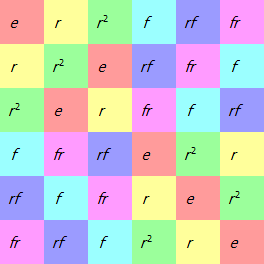
\includegraphics{S3table.png}
\end{minipage}\\
\hspace*{0.25in}
\begin{minipage}{2.5in}
$\begin{array}
[c]{rcl}%
&S_{3}&\\
r & = &
\begin{pmatrix}1&2&3\\2&3&1\end{pmatrix}\\
f & = &
\begin{pmatrix}1&2&3\\1&3&2\end{pmatrix}\\
\end{array}
$
\end{minipage}


\vspace{0.25in}

\centerline{\begin{minipage}{2.0in}
\small{Version 4.00\newline June 23, 2021}
\end{minipage}}

\raggedbottom\clearpage\pagenumbering{arabic} \vspace*{0.1in}

\noindent The first version of these notes was written for a first-year
graduate algebra course. As in most such courses, the notes concentrated on
abstract groups and, in particular, on finite groups. However, it is not as
abstract groups that most mathematicians encounter groups, but rather as
algebraic groups, topological groups, or Lie groups, and it is not just the
groups themselves that are of interest, but also their linear representations.
It is my intention (one day) to expand the notes to take account of this, and
to produce a volume that, while still modest in size (c200 pages), will
provide a more comprehensive introduction to group theory for beginning
graduate students in mathematics, physics, and related fields.

\vfill \noindent BibTeX information
\begin{verbatim}
@misc{milneGT,
  author={Milne, James S.},
  title={Group Theory (v4.00)},
  year={2021},
  note={Available at www.jmilne.org/math/},
  pages={139}
}
\end{verbatim}

\vfill


\noindent Please send comments and corrections to me at jmilne at umich dot edu.

\noindent v2.01 (August 21, 1996). First version on the web; 57 pages.

\noindent v2.11 (August 29, 2003). Revised and expanded; numbering; unchanged; 85 pages.

\noindent v3.00 (September 1, 2007). Revised and expanded; 121 pages.

\noindent v3.16 (July 16, 2020). Revised and expanded; 137 pages.

\noindent v4.00 (June 23, 2021). Made work (including source code) available
under Creative Commons licence.
\vfill


\noindent The multiplication table of $S_{3}$ on the front page was produced
by Group Explorer. \vfill

\noindent Version 4.0 is published under a Creative Commons
Attribution-NonCommercial-ShareAlike 4.0 International licence
(CC BY-NC-SA 4.0).

\bigskip

\noindent Licence information:
\href{https://creativecommons.org/licenses/by-nc-sa/4.0/}{https://creativecommons.org/licenses/by-nc-sa/4.0}

\bigskip

\noindent Copyright \copyright 1996--2021 J.S. Milne.




\setcounter{page}{2}
\clearpage\pagestyle{plain}
\vspace*{-0.5in}\tableoc


\clearpage


\subsection{Notation.}

\sloppy We use the standard (Bourbaki) notation: $\mathbb{N}=\{0,1,2,\ldots\}$;
$\mathbb{Z}$ is the ring of integers; $\mathbb{Q}{}$ is the field of rational
numbers; $\mathbb{R}{}$ is the field of real numbers; $\mathbb{C}{}$ is the
field of complex numbers; $\mathbb{F}_{q}$ is a finite field with $q$
elements, where $q$ is a power of a prime number. In particular,
$\mathbb{F}_{p}=\mathbb{Z}{}/p\mathbb{Z}{}$ for $p$ a prime number.

For integers $m$ and $n$, $m|n$ means that $m$ divides $n$, i.e., $n\in
m\mathbb{Z}{}$. Throughout the notes, $p$ is a prime number, i.e.,
$p=2,3,5,7,11,\ldots,1000000007,\ldots$.

Given an equivalence relation, $[\ast]$ denotes the equivalence class
containing $\ast$. The empty set is denoted by $\emptyset$. The cardinality of
a set $S$ is denoted by $|S|$ (so $|S|$ is the number of elements in $S$ when
$S$ is finite). Let $I$ and $A$ be sets; a family of elements of\emph{\ }%
$A$\emph{\ }indexed by $I$, denoted $(a_{i})_{i\in I}$, is a function
$i\mapsto a_{i}\colon I\rightarrow A$.\footnote{A family should be
distinguished from a set. For example, if $f$ is the function $\mathbb{Z}%
{}\rightarrow\mathbb{Z}{}/3\mathbb{Z}{}$ sending an integer to its equivalence
class, then $\{f(i)\mid i\in\mathbb{Z\}}$ is a set with three elements whereas
$(f(i))_{i\in\mathbb{Z}{}}$ is family with an infinite index set.}

Rings are required to have an identity element $1$, and homomorphisms of rings
are required to take $1$ to $1$. An element $a$ of a ring is a unit if it has
an inverse (element $b$ such that $ab=1=ba$). The identity element of a ring
is required to act as $1$ on a module over the ring.

\noindent$%
\begin{array}
[c]{ll}%
X\subset Y & X\text{ is a subset of }Y\text{ (not necessarily proper);}\\
X\overset{\df}{=}Y & X\text{ is defined to be }Y\text{, or
  equals }Y \\
& \text{ by definition;}\\
X\approx Y & X\text{ is isomorphic to }Y\text{;}\\
X\simeq Y & X\text{ and }Y\text{ are canonically isomorphic (or}\\
& \text{ there is a
given or unique isomorphism);}%
\end{array}
$

\subsection{Prerequisites}

An undergraduate \textquotedblleft abstract algebra\textquotedblright\ course.

\subsection{Computer algebra programs}

GAP is an open source computer algebra program, emphasizing computational
group theory. To get started with GAP, I recommend going to Alexander Hulpke's
page \href{http://www.math.colostate.edu/~hulpke/CGT/education.html}{here},
where you will find versions of GAP for both Windows and Macs and a guide
\textquotedblleft Abstract Algebra in GAP\textquotedblright. The Sage page
\href{http://www.sagemath.org/}{here} provides a front end for GAP and other
programs. I also recommend N. Carter's \textquotedblleft Group
Explorer\textquotedblright%
\ \href{https://nathancarter.github.io/group-explorer/index.html}{here} for
exploring the structure of groups of small order. Earlier versions of these
notes (v3.02) described how to use Maple for computations in group theory.

\subsection{Acknowledgements}

\bsmall
I thank the following for providing corrections and comments for earlier
versions of these notes: V.V. Acharya; Yunghyun Ahn; Max Black; Tony Bruguier; Vigen
Chaltikyan; Dustin Clausen; Beno\^{\i}t Claudon; Keith Conrad; Demetres
Christofides; Adam Glesser; Darij Grinberg; Sylvan Jacques; Martin Klazar;
Thomas Lamm; Mark Meckes; Max Menzies; Victor Petrov; Flavio Poletti; Diego Silvera;
Efthymios Sofos; Dave Simpson; David Speyer; Kenneth Tam; Robert Thompson;
Bhupendra Nath Tiwari; Leandro Vendramin; Michiel Vermeulen.

Also, I have benefited from the posts to mathoverflow by Richard Borcherds,
Robin Chapman, Steve Dalton, Leonid Positselski, Noah Snyder, Richard Stanley,
Qiaochu Yuan, and others.

A reference \textbf{monnnn} means question nnnn on mathoverflow.net and
\textbf{sxnnnn} similarly refers to math.stackexchange.com. \esmall


\clearpage\thispagestyle{empty} \vspace*{0in}

\bsmall


\begin{quote}
The theory of groups of finite order may be said to date from the time of
Cauchy. To him are due the first attempts at classification with a view to
forming a theory from a number of isolated facts. Galois introduced into the
theory the exceedingly important idea of a [normal] sub-group, and the
corresponding division of groups into simple and composite. Moreover, by
shewing that to every equation of finite degree there corresponds a group of
finite order on which all the properties of the equation depend, Galois
indicated how far reaching the applications of the theory might be, and
thereby contributed greatly, if indirectly, to its subsequent developement.

Many additions were made, mainly by French mathematicians, during the middle
part of the [nineteenth] century. The first connected exposition of the theory
was given in the third edition of M. Serret's \textquotedblleft\textit{Cours
d'Alg\`{e}bre Sup\'{e}rieure,}\textquotedblright\ which was published in 1866.
This was followed in 1870 by M. Jordan's \textquotedblleft\textit{Trait\'{e}
des substitutions et des \'{e}quations alg\'{e}briques.}\textquotedblright%
\ The greater part of M. Jordan's treatise is devoted to a developement of the
ideas of Galois and to their application to the theory of equations.

No considerable progress in the theory, as apart from its applications, was
made till the appearance in 1872 of Herr Sylow's memoir \textquotedblleft%
\textit{Th\'{e}or\`{e}mes sur les groupes de substitutions}\textquotedblright%
\ in the fifth volume of the \textit{Mathematische Annalen.} Since the date of
this memoir, but more especially in recent years, the theory has advanced continuously.

\bigskip\hfill W. Burnside, Theory of Groups of Finite Order, 1897.
\end{quote}

\vfill


\begin{quote}
Galois introduced the concept of a normal subgroup in 1832, and Camille Jordan
in the preface to his \textit{Trait\'{e}\ldots} in 1870 flagged Galois'
distinction between groupes simples and groupes compos\'{e}es as the most
important dichotomy in the theory of permutation groups. Moreover, in the
\textit{Trait\'{e}}, Jordan began building a database of finite simple groups
--- the alternating groups of degree at least $5$ and most of the classical
projective linear groups over fields of prime cardinality. Finally, in 1872,
Ludwig Sylow published his famous theorems on subgroups of prime power order.

\bigskip\hfill R. Solomon, Bull. Amer. Math. Soc., 2001.
\end{quote}

\vfill


Why are the finite simple groups classifiable?

\begin{quote}
It is unlikely that there is any easy reason why a classification is possible,
unless someone comes up with a completely new way to classify groups. One
problem, at least with the current methods of classification via centralizers
of involutions, is that every simple group has to be tested to see if it leads
to new simple groups containing it in the centralizer of an involution. For
example, when the baby monster was discovered, it had a double cover, which
was a potential centralizer of an involution in a larger simple group, which
turned out to be the monster. The monster happens to have no double cover so
the process stopped there, but without checking every finite simple group
there seems no obvious reason why one cannot have an infinite chain of larger
and larger sporadic groups, each of which has a double cover that is a
centralizer of an involution in the next one. Because of this problem (among
others), it was unclear until quite late in the classification whether there
would be a finite or infinite number of sporadic groups.

\bigskip\hfill Richard Borcherds, mo38161.
\end{quote}

\esmall %\vfill


%\clearpage
%\renewcommand\subsectionmark{\markright{}}
\pagestyle{ruled} \makeevenfoot{ruled}{}{}{}{} \makeoddfoot{ruled}{}{}{}{}
\makeevenhead{ruled}{\thepage}{\scshape \leftmark}{} \makeoddhead{ruled}{}{\rightmark}{\thepage}

\chapter{Basic Definitions and Results}

\setlength{\epigraphwidth}{3in} \setlength{\epigraphrule}{0pt}
\epigraph{\textit{The axioms for a group are short and natural\ldots.
Yet somehow hidden behind these axioms is the monster simple group,
a huge and extraordinary mathematical object, which appears to rely
on numerous bizarre coincidences to exist. The axioms for groups
give no obvious hint that anything like this exists.}} {Richard Borcherds, in
\textit{Mathematicians: An Outer View\ldots.}}

\vspace{-1cm}\setlength{\epigraphwidth}{3in} \setlength{\epigraphrule}{0pt}
\epigraph{\textit{The one thing I would really like to know before I
die is why the monster group exists.}} {John Conway, in a 2014 interview on
Numberphile.}

Group theory is the study of symmetries.

\section{Definitions and examples}

\begin{definition}
\label{bd1} A \emph{group}%
\index{group}
is a set $G$ together with a binary operation
\[
(a,b)\mapsto a\ast b\colon G\times G\rightarrow G
\]
satisfying the following conditions:

\begin{description}
\item[G1:] (associativity) for all $a,b,c\in G$,
\[
(a\ast b)\ast c=a\ast(b\ast c);
\]


\item[G2:] (existence of a neutral element) there exists an element $e\in G$
such that
\begin{equation}
a\ast e=a=e\ast a \label{e14}%
\end{equation}
for all $a\in G$;

\item[G3:] (existence of inverses) for each $a\in G$, there exists an
$a^{\prime}\in G$ such that
\[
a\ast a^{\prime}=e=a^{\prime}\ast a.
\]

\end{description}
\end{definition}

\noindent We usually abbreviate $(G,\ast)$ to $G$. Also, we usually write $ab$
for $a\ast b$ and $1$ for $e$; alternatively, we write $a+b$ for $a\ast b$ and
0 for $e$. In the first case, the group is said to be \emph{multiplicative}%
\index{group!multiplicative}%
, and in the second, it is said to be \emph{additive}%
\index{group!additive}%
.

\begin{plain}
\label{bd2}In the following, $a,b,\ldots$ are elements of a group $G$.

\begin{enumerate}
\item An element $e$ satisfying (\ref{e14}) is called a \emph{neutral element}%
\index{element!neutral}%
. If $e^{\prime}$ is a second such element, then $e^{\prime}=e\ast e^{\prime
}=e$. In fact, $e$ is the unique element of $G$ satisfying $x\ast x=x$ (apply G3).

\item If $b\ast a=e$ and $a\ast c=e$, then
\[
b=b\ast e=b\ast(a\ast c)=(b\ast a)\ast c=e\ast c=c.
\]
Hence the element $a^{\prime}$ in (G3) is uniquely determined by $a$. We call
it the \emph{inverse\/}%
\index{inverse}
of $a$, and denote it $a^{-1}$ (or the \emph{negative\/}%
\index{negative}
of $a$, and denote it $-a$).

\item Note that (G1) shows that the product of any ordered triple $a_{1}$,
$a_{2}$, $a_{3}$ of elements of $G$ is unambiguously defined: whether we form
$a_{1}a_{2}$ first and then $(a_{1}a_{2})a_{3}$, or $a_{2}a_{3}$ first and
then $a_{1}(a_{2}a_{3})$, the result is the same. In fact, (G1) implies that
the product of any ordered $n$-tuple $a_{1}$, $a_{2}$,\ldots, $a_{n}$ of
elements of $G$ is unambiguously defined. We prove this by induction on $n$.
In one multiplication, we might end up with%
\begin{equation}
(a_{1}\cdots a_{i})(a_{i+1}\cdots a_{n}) \label{e3}%
\end{equation}
as the final product, whereas in another we might end up with%
\begin{equation}
(a_{1}\cdots a_{j})(a_{j+1}\cdots a_{n}). \label{e4}%
\end{equation}
Note that the expression within each pair of parentheses is well defined
because of the induction hypotheses. Thus, if $i=j$, (\ref{e3}) equals
(\ref{e4}). If $i\neq j$, we may suppose $i<j$. Then%
\begin{align*}
  &(a_{1}\cdots a_{i})(a_{i+1}\cdots a_{n}) \\
  =&(a_{1}\cdots a_{i})\left(
(a_{i+1}\cdots a_{j})(a_{j+1}\cdots a_{n})\right) \\
 &(a_{1}\cdots a_{j})(a_{j+1}\cdots a_{n})  \\
  =&\left(  (a_{1}\cdots
a_{i})(a_{i+1}\cdots a_{j})\right)  (a_{j+1}\cdots a_{n})
\end{align*}
and the expressions on the right are equal because of (G1).

\item The inverse of $a_{1}a_{2}\cdots a_{n}$ is $a_{n}^{-1}a_{n-1}^{-1}\cdots
a_{1}^{-1}$, i.e., the inverse of a product is the product of the inverses in
the reverse order.

\item (G3) implies that the cancellation laws hold in groups,
\[
ab=ac\implies b=c,\qquad ba=ca\implies b=c
\]
(multiply on left or right by $a^{-1}$). Conversely, if $G$ is \textit{finite}%
, then the cancellation laws imply (G3): the map $x\mapsto ax\colon
G\rightarrow G$ is injective, and hence (by counting) bijective; in
particular, $e$ is in the image, and so $a$ has a right inverse; similarly, it
has a left inverse, and the argument in (b) above shows that the two inverses
are equal.
\end{enumerate}
\end{plain}

Two groups $(G,\ast)$ and $(G^{\prime},\ast^{\prime})$ are \emph{isomorphic\/}%
\index{isomorphism!of groups}
if there exists a one-to-one correspondence $a\leftrightarrow a^{\prime}$,
$G\leftrightarrow G^{\prime}$, such that $(a\ast b)^{\prime}=a^{\prime}%
\ast^{\prime}b^{\prime}$ for all $a,b\in G$.

The \emph{order}%
\index{order!of a group}
$|G|$ of a group $G$ is its cardinality. A finite group whose order is a power
of a prime $p$ is called a $p$\emph{-group}.%
\index{group!p@$p$}%


For an element $a$ of a group $G$, define
\[
a^{n}=\left\{
\begin{array}
[c]{lll}%
aa\cdots a & n>0 & (n\text{ copies of }a)\\
e & n=0 & \\
a^{-1}a^{-1}\cdots a^{-1} & n<0 & \text{(}|n|\text{ copies of }a^{-1}\text{)}%
\end{array}
\right.
\]
The usual rules hold:
\begin{equation}
a^{m}a^{n}=a^{m+n},\quad(a^{m})^{n}=a^{mn},\quad\text{all }m,n\in\mathbb{Z}{}.
\label{e1}%
\end{equation}
It follows from (\ref{e1}) that the set
\[
\{n\in\mathbb{Z}\mid a^{n}=e\}
\]
is an ideal in $\mathbb{Z}$, and so equals $m\mathbb{Z}{}$ for some integer
$m\geq0$. When $m=0$, $a^{n}\neq e$ unless $n=0$, and $a$ is said to have
\emph{infinite order}%
\index{order!of an element}%
. When $m\neq0$, it is the smallest integer $m>0$ such that $a^{m}=e$, and $a$
is said to have \emph{finite order }$m$. In this case, $a^{-1}=a^{m-1}$, and%

\[
a^{n}=e\iff m|n.
\]


\subsection{Examples}

\begin{plain}
\label{bd3a}Let $C_{\infty}$ be the group $(\mathbb{Z}{},+)$, and, for an
integer $m\geq1$, let $C_{m}$ be the group $(\mathbb{Z}/m\mathbb{Z}{},+)$.%
\index{Cm@$C_{m}$}%

\end{plain}

\begin{plain}
\label{bd3b}\emph{Permutation groups.\/} Let $S$ be a set and let $\Sym(S)$ be
the set of bijections $\alpha\colon S\rightarrow S$. We define the product of
two elements of $\Sym(S)$ to be their composite:
\[
\alpha\beta=\alpha\circ\beta.
\]
In other words, $(\alpha\beta)(s)=\alpha(\beta(s))$ for all $s\in S$. For any
$\alpha,\beta,\gamma\in\Sym(S)$ and $s\in S$,
\begin{equation}
\begin{aligned}
  &\left(  (\alpha\circ\beta)\circ\gamma\right)  (s)\\
  =&(\alpha\circ\beta
  )(\gamma(s))\\
  =&\alpha(\beta(\gamma(s)))\\
  =&\left(  \alpha\circ(\beta\circ
\gamma)\right)  (s), \end{aligned}
\label{e11}%
\end{equation}
and so associativity holds. The identity map $s\mapsto s$ is an identity
element for $\Sym(S)$, and inverses exist because we required the elements of
$\Sym(S)$ to be bijections. Therefore $\Sym(S)$ is a group, called the
\emph{group of symmetries}%
\index{group!of symmetries}
of $S$. For example, the \emph{permutation group on} $n$ \emph{letters}%
\index{group!permutation}%
\index{Sn@$S_{n}$}%
\/ $S_{n}$ is defined to be the group of symmetries of the set $\{1,...,n\}$
--- it has order $n!$.
\end{plain}

\begin{plain}
\label{bd3c}When $G$ and $H$ are groups, we can construct a new group $G\times
H$, called the \emph{(direct) product\/}%
\index{product!direct}
of $G$ and $H$. As a set, it is the cartesian product of $G$ and $H$, and
multiplication is defined by
\[
(g,h)(g^{\prime},h^{\prime})=(gg^{\prime},hh^{\prime}).
\]

\end{plain}

\begin{plain}
\label{bd3d}A group $G$ is \emph{commutative}%
\index{group!commutative}%
\/ (or \emph{abelian}%
\index{group!abelian}%
\/)\footnote{\textquotedblleft Abelian group\textquotedblright\ is more common
than \textquotedblleft commutative group\textquotedblright, but I prefer to
use descriptive names.} if
\[
ab=ba,\quad\text{all }a,b\in G.
\]
In a commutative group, the product of any finite (not necessarily ordered)
family $S$ of elements is well defined, for example, the empty product is $e$.
Usually, we write commutative groups additively. With this notation, Equation
(\ref{e1}) becomes:%
\[
ma+na=(m+n)a,\quad m(na)=mna.
\]
When $G$ is commutative,
\[
m(a+b)=ma+mb\text{ for }m\in\mathbb{Z}{}\text{ and }a,b\in G\text{,}%
\]
and so the map%
\[
(m,a)\mapsto ma\colon\mathbb{Z}{}\times G\rightarrow G
\]
makes $G$ into a $\mathbb{Z}{}$-module. In a commutative group $G$, the
elements of finite order form a subgroup $G_{\text{tors}}$ of $G$, called the
\emph{torsion subgroup}.%
\index{subgroup!torsion}%

\end{plain}

\begin{plain}
\label{bd3e}Let $F$ be a field. The $n\times n$ matrices with coefficients in
$F$ and nonzero determinant form a group%
\index{GLn@$\GL_{n}(F)$}
$\GL_{n}(F)$ called the \emph{general linear group of degree} $n$.%
\index{group!general linear}
For a finite-dimensional $F$-vector space $V$, the $F$-linear automorphisms of
$V$ form a group $\GL(V)$ called the \emph{general linear group of} $V$. Note
that if $V$ has dimension $n$, then the choice of a basis determines an
isomorphism $\GL(V)\rightarrow\GL_{n}(F)$ sending an automorphism to its
matrix with respect to the basis.
\end{plain}

\begin{plain}
\label{bd3f}Let $V$ be a finite-dimensional vector space over a field $F$. A
bilinear form on $V$ is a mapping $\phi\colon V\times V\rightarrow F$ that is
linear in each variable. An \emph{automorphism}%
\index{automorphism!of a bilinear form}
of such a $\phi$ is an isomorphism $\alpha\colon V\rightarrow V$ such that%
\begin{equation}
\phi(\alpha v,\alpha w)=\phi(v,w)\text{ for all }v,w\in V. \label{e8}%
\end{equation}
The automorphisms of $\phi$ form a group $\Aut(\phi)$. Let $\{e_{1}%
,\ldots,e_{n}\}$ be a basis for $V$, and let%
\[
P=(\phi(e_{i},e_{j}))_{1\leq i,j\leq n}%
\]
be the matrix of $\phi$. The choice of the basis identifies $\Aut(\phi)$ with
the group of invertible matrices $A$ such that\footnote{When we use the basis
to identify $V$ with $F^{n}$, the pairing $\phi$ becomes%
\[
\left(
\begin{smallmatrix}
\vphantom{b}a_{1}\\
\vdots\\
\vphantom{b}a_{n}%
\end{smallmatrix}
\right)  ,\left(
\begin{smallmatrix}
b_{1}\\
\vdots\\
b_{n}%
\end{smallmatrix}
\right)  \mapsto(a_{1},\ldots,a_{n})\cdot P\cdot\left(
\begin{smallmatrix}
b_{1}\\
\vdots\\
b_{n}%
\end{smallmatrix}
\right)  .
\]
If $A$ is the matrix of $\alpha$ with respect to the basis, then $\alpha$
corresponds to the map $\left(
\begin{smallmatrix}
a_{1}\\
\vdots\\
a_{n}%
\end{smallmatrix}
\right)  \mapsto A\left(
\begin{smallmatrix}
a_{1}\\
\vdots\\
a_{n}%
\end{smallmatrix}
\right)  .$Therefore, (\ref{e8}) becomes the statement that%
\begin{align*}
(a_{1},\ldots,a_{n})\cdot A^{\mathrm{T}}\cdot P\cdot A\cdot\left(
\begin{smallmatrix}
b_{1}\\
\vdots\\
b_{n}%
\end{smallmatrix}
\right)  =(a_{1},\ldots,a_{n})\cdot P\cdot\left(
\begin{smallmatrix}
b_{1}\\
\vdots\\
b_{n}%
\end{smallmatrix}
\right)  \\
\text{ for all }\left(
\begin{smallmatrix}
\vphantom{b}a_{1}\\
\vdots\\
\vphantom{b}a_{n}%
\end{smallmatrix}
\right)  ,\left(
\begin{smallmatrix}
b_{1}\\
\vdots\\
b_{n}%
\end{smallmatrix}
\right)  \in F^{n}.
\end{align*}
On examining this statement on the standard basis vectors for $F^{n}$, we see
that it is equivalent to (\ref{e9}).}%
\begin{equation}
A^{\text{\textrm{T}}}\cdot P\cdot A=P\text{.} \label{e9}%
\end{equation}


When $\phi$ is symmetric, i.e.,
\[
\phi(v,w)=\phi(w,v)\text{ all }v,w\in V,
\]
and nondegenerate, $\Aut(\phi)$ is called the \emph{orthogonal group}%
\index{group!orthogonal}
of $\phi$.

When $\phi$ is skew-symmetric, i.e.,%
\[
\phi(v,w)=-\phi(w,v)\text{ all }v,w\in V,
\]
and nondegenerate, $\Aut(\phi)$ is called the \emph{symplectic group}%
\index{group!symplectic}
of $\phi$. In this case, there exists a basis for $V$ for which the matrix of
$\phi$ is%
\[
J_{2m}=%
\begin{pmatrix}
0 & I_{m}\\
-I_{m} & 0
\end{pmatrix}
,\quad2m=n,
\]
and the group of invertible matrices $A$ such that%
\[
A^{\mathrm{T}}J_{2m}A=J_{2m}%
\]
is called the symplectic group $\SP_{2m}$.
\end{plain}

\begin{remark}
\label{bd3g}A set $S$ together with a binary operation $(a,b)\mapsto a\cdot
b\colon S\times S\rightarrow S$ is called a \emph{magma}. When the binary
operation is associative, $(S,\cdot)$ is called a \emph{semigroup}. The
product%
\[
\tstyle\prod A\overset{\textup{{\tiny def}}}{=}a_{1}\cdots a_{n}%
\]
of any sequence $A=(a_{i})_{1\leq i\leq n}$ of elements in a semigroup $S$ is
well-defined (see \ref{bd2}(c)), and for any pair $A$ and $B$ of such
sequences,%
\begin{equation}
\tstyle\left(  \prod A\right)  \left(  \prod B\right)  =\prod\left(  A\sqcup
B\right)  \text{.} \label{e29}%
\end{equation}
Let $\emptyset$ be the empty sequence, i.e., the sequence of elements in $S$
indexed by the empty set. What should $\prod\emptyset$ be? Clearly, we should
have%
\begin{align*}
\tstyle\left(  \prod\emptyset\right)  \left(  \prod A\right)  =\prod\left(
\emptyset\sqcup A\right)  =\prod A\\
=\prod\left(  A\sqcup\emptyset\right)
=\left(  \prod A\right)  \left(  \prod\emptyset\right)  .
\end{align*}
In other words, $\prod\emptyset$ should be a neutral element. A semigroup with
a neutral element is called a \emph{monoid}. In a monoid, the product of any
finite (possibly empty) sequence of elements is well-defined, and (\ref{e29}) holds.
\end{remark}

\begin{aside}
\label{bd3z}(a) The group conditions (G2,G3) can be replaced by the following
weaker conditions (existence of a left neutral element and left inverses):
(G2$^{\prime}$) there exists an $e$ such that $e\ast a=a$ for all $a$;
(G3$^{\prime}$) for each $a\in G$, there exists an $a^{\prime}\in G$ such that
$a^{\prime}\ast a=e$. To see that these imply (G2) and (G3), let $a\in G$, and
apply (G3$^{\prime}$) to find $a^{\prime}$ and $a^{\prime\prime}$ such that
$a^{\prime}\ast a=e$ and $a^{\prime\prime}\ast a^{\prime}=e$. Then%
\begin{align*}
a\ast a^{\prime}=e\ast(a\ast a^{\prime})=(a^{\prime\prime}\ast a^{\prime}%
)\ast(a\ast a^{\prime})\\
=a^{\prime\prime}\ast\left(  (a^{\prime}\ast a)\ast
a^{\prime}\right)  =a^{\prime\prime}\ast a^{\prime}=e,
\end{align*}
whence (G3), and%
\[
a=e\ast a=(a\ast a^{\prime})\ast a=a\ast(a^{\prime}\ast a)=a\ast e,
\]
whence (G2).

(b) A group can be defined to be a set $G$ with a binary operation $\ast$
satisfying the following conditions: (g1) $\ast$ is associative; (g2) $G$ is
nonempty; (g3) for each $a\in G$, there exists an $a^{\prime}\in G$ such that
$a^{\prime}\ast a$ is neutral. As there is at most one neutral element in a
set with an associative binary operation, these conditions obviously imply
those in (a). They are minimal in the sense that there exist sets with a
binary operation satisfying any two of them but not the third. For example,
$(\mathbb{N}{},+)$ satisfies (g1) and (g2) but not (g3); the empty set
satisfies (g1) and (g3) but not (g2); the set of integers with $m*n=m-n$
satisfies (g2) and (g3) but not (g1).
\end{aside}

\section{Multiplication tables}

A binary operation on a finite set can be described by its multiplication
table:%
\index{table!multiplication}
\[%
\begin{tabular}
[c]{|c|ccccc|}\hline
& $e$ & $a$ & $b$ & $c$ & $\ldots$\\\hline
$e$ & $ee$ & $ea$ & $eb$ & $ec$ & $\ldots$\\
$a$ & $ae$ & $a^{2}$ & $ab$ & $ac$ & $\ldots$\\
$b$ & $be$ & $ba$ & $b^{2}$ & $bc$ & $\ldots$\\
$c$ & $ce$ & $ca$ & $cb$ & $c^{2}$ & $\ldots$\\
$\vdots$ & $\vdots$ & $\vdots$ & $\vdots$ & $\vdots$ & \\\hline
\end{tabular}
\ \ \
\]


The element $e$ is an identity element if and only if the first row and column
of the table simply repeat the elements. Inverses exist if and only if each
element occurs exactly once in each row and in each column (see \ref{bd2}e).
If there are $n$ elements, then verifying the associativity law requires
checking $n^{3}$ equalities.

For the multiplication table of $S_{3}$, see the front page. Note that each
colour occurs exactly once in each row and and each column.

This suggests an algorithm for finding all groups of a given finite order $n$,
namely, list all possible multiplication tables and check the axioms. Except
for very small $n$, this is not practical! The table has $n^{2}$ positions,
and if we allow each position to hold any of the $n$ elements, then that gives
a total of $n^{n^{2}}$ possible tables very few of which define groups. For
example, there are $8^{64}=\allowbreak6277\,\allowbreak
101\,735\,386\,\allowbreak680\,763\,835\,\allowbreak789\,423\,207\,\allowbreak
666\,416\,102\,\allowbreak355\,444\,464\,\allowbreak034\,512\,896\allowbreak$
binary operations on a set with $8$ elements, but only five isomorphism
classes of groups of order $8$ (see \ref{ga18e}).

\section{Subgroups}

\begin{proposition}
\label{bd4} Let $S$ be a nonempty subset of a group $G$. If

\begin{description}
\item[S1:] $a,b\in S\implies ab\in S$, and

\item[S2:] $a\in S\implies a^{-1}\in S,$
\end{description}

\noindent then the binary operation on $G$ makes $S$ into a group.
\end{proposition}

\begin{proof}
\vskip-1em (S1) implies that the binary operation on $G$ defines a binary
operation $S\times S\rightarrow S$ on $S$, which is automatically associative.
By assumption $S$ contains at least one element $a$, its inverse $a^{-1}$, and
the product $e=aa^{-1}$. Finally (S2) shows that the inverses of elements in
$S$ lie in $S$.
\end{proof}

A nonempty subset $S$ satisfying (S1) and (S2) is called a \emph{subgroup\/}%
\index{subgroup}
of $G$. When $S$ is finite, condition (S1) implies (S2): let $a\in S$; then
$\{a,a^{2},\ldots\}\subset S$, and so $a$ has finite order, say $a^{n}=e$; now
$a^{-1}=a^{n-1}\in S$. The example $(\mathbb{N},+)\subset(\mathbb{Z},+)$ shows
that (S1) does not imply (S2) when $S$ is infinite.

\begin{example}
\label{bd4e}The \emph{centre\/}%
\index{centre!of a group}
of a group $G$ is the subset%
\[
Z(G)=\{g\in G\mid gx=xg\text{ for all }x\in G\}.
\]
It is a subgroup of $G$.
\end{example}

\begin{proposition}
\label{bd5} An intersection of subgroups of $G$ is a subgroup of $G.$
\end{proposition}

\begin{proof}
\vskip-1em It is nonempty because it contains $e$, and (S1) and (S2) obviously hold.
\end{proof}

\begin{remark}
\label{bd6} It is generally true that an intersection of subobjects of an
algebraic object is a subobject. For example, an intersection of subrings of a
ring is a subring, an intersection of submodules of a module is a submodule,
and so on.
\end{remark}

\begin{proposition}
\label{bd7} For any subset $X$ of a group $G$, there is a smallest subgroup of
$G$ containing $X$. It consists of all finite products of elements of $X$ and
their inverses (repetitions allowed).
\end{proposition}

\begin{proof}
\vskip-1em The intersection $S$ of all subgroups of $G$ containing $X$ is
again a subgroup containing $X$, and it is evidently the smallest such group.
Clearly $S$ contains with $X$, all finite products of elements of $X$ and
their inverses. But the set of such products satisfies (S1) and (S2) and hence
is a subgroup containing $X$. It therefore equals $S$.
\end{proof}

The subgroup $S$ given by the proposition is denoted $\langle X\rangle$, and
is called the \emph{subgroup generated by} $X$.%
\index{subgroup!generated by a set}
For example, $\langle\emptyset\rangle=\{e\}$. If every element of $X$ has
finite order, for example, if $G$ is finite, then the set of all finite
products of elements of $X$ is already a group and so equals $\langle
X\rangle$.

We say that $X$ \emph{generates}%
\index{generates}
$G$ if $G=\langle X\rangle$, i.e., if every element of $G$ can be written as a
finite product of elements from $X$ and their inverses. Note that the order of
an element $a$ of a group is the order of the subgroup $\langle a\rangle$ it generates.

\subsection{Examples}

\begin{plain}
\label{bd8a}\emph{The cyclic groups. }A group is said to be \emph{cyclic}%
\index{group!cyclic}%
\emph{\/} if it is generated by a single element, i.e., if $G=\langle
r\rangle$ for some $r\in G$. If $r$ has finite order $n$, then
\[
G=\{e,r,r^{2},...,r^{n-1}\}\approx C_{n},\quad r^{i}\leftrightarrow i\mod n,
\]
and $G$ can be thought of as the group of rotational symmetries about the
centre of a regular polygon with $n$-sides. If $r$ has infinite order, then
\[
G=\{\ldots,r^{-}{}^{i},\ldots,r^{-1},e,r,\ldots,r^{i},\ldots\}\approx
C_{\infty},\quad r^{i}\leftrightarrow i.
\]
Thus, up to isomorphism, there is exactly one cyclic group of order $n$ for
each $n\leq\infty$. In future, we shall loosely use $C_{n}$ to denote any
cyclic group of order $n$ (not necessarily $\mathbb{Z}{}/n\mathbb{Z}{}$ or
$\mathbb{Z}{}$).
\end{plain}

\begin{plain}
\label{bd8b}\emph{The dihedral groups} $D_{n}$.\footnote{This group is denoted
$D_{2n}$ or $D_{n}$ depending on whether the author is viewing it abstractly
or concretely as the symmetries of an $n$-polygon (or perhaps on whether the
author is a group theorist or not; see mo48434).}%
\index{group!dihedral}%
\index{Dn@$D_{n}$}
For $n\geq3$, $D_{n}$ is the group of symmetries of a regular polygon with
$n$-sides.\footnote{More formally, $D_{n}$ can be defined to be the subgroup
of $S_{n}$ generated by $r\colon i\mapsto i+1$ (mod $n)$ and $s\colon i\mapsto
n+2-i$ (mod $n$). Then all the statements concerning $D_{n}$ can proved
without appealing to geometry.} Number the vertices $1,\ldots,n$ in the
counterclockwise direction. Let $r$ be the rotation through $2\pi/n$ about the
centre of polygon (so $i\mapsto i+1\mod
n)$, and let $s$ be the reflection in the line (= rotation about the line)
through the vertex $1$ and the centre of the polygon (so $i\mapsto
n+2-i\mod n$). For example, the pictures \bigskip

\noindent\begin{minipage}{1.3in}
\begin{tikzpicture}
\path (0,0) coordinate (origin);
\path (90:2cm) coordinate (P1);
\path (210:2cm) coordinate (P2);
\path (330:2cm) coordinate (P3);
\draw (P1) -- (P2) -- (P3) -- cycle;
\draw[dashed] (0,-1.8) -- (0,2.6);
%%now for the loop at top
\draw[->,>=angle 90] (-0.6,2.6) arc (180:360:0.6cm and 0.4cm);
%%now for the arc at the side
\path (P3) ++(130:3.5cm) coordinate (o3);
\draw[->,>=angle 90] (o3) arc (130:170:3.5cm);
%%finally some text
\path (origin) node {$\bullet$}
(P1) +(-4pt,-3pt) node [anchor=north west] {$1$}
(P2) +(3pt,0pt) node [anchor=south west] {$2$}
(P3) +(-3pt,0pt) node [anchor=south east]{$3$}
(-1.3,1) node {$r$}
(0.65,2.25) node {$s$};
\end{tikzpicture}
\end{minipage}
\begin{minipage}{1in}
\begin{align*}
s  & =\left\{
\begin{array}
[c]{c}%
1\leftrightarrow1\\
2\leftrightarrow3
\end{array}
\right.  \\
r  & =1\rightarrow2\rightarrow3\rightarrow1
\end{align*}
\end{minipage}
\\
\begin{minipage}{1.7in}
\begin{tikzpicture}
\path (0,0) coordinate (origin);
\path (90:2cm) coordinate (P1);
\path (180:2cm) coordinate (P2);
\path (270:2cm) coordinate (P3);
\path (360:2cm) coordinate (P4);
\draw (P1) -- (P2) -- (P3) -- (P4) -- cycle;
\draw[dashed] (0,-2.2) -- (0,2.6);
%%Now for the arc at the top
\draw[->,>=angle 90] (-0.6,2.5) arc (180:360:0.6cm and 0.4cm);
%%Now for the arc at the side
\path (1,-1) coordinate (o1);
\path (o1) +(118:3.25cm) coordinate (o2);
\draw[->,>=angle 90] (o2) arc (118:152:3.25cm);
%%finally the text
\path (origin) node {$\bullet$}
(P1) +(-3pt,-1pt) node [anchor=north west] {$1$}
(P2) +(2pt,0) node [anchor=west] {$2$}
(P3) +(-3pt,3pt) node [anchor=south west]{$3$}
(P4)  node [anchor=east] {$4$}
(-1.4,1.4) node {$r$}
(0.7,2.2) node {$s$};
\end{tikzpicture}
\end{minipage}
\begin{minipage}{1.5in}
\begin{align*}
s  & =\left\{
\begin{array}
[c]{c}%
1\leftrightarrow1\\
2\leftrightarrow4\\
3\leftrightarrow3
\end{array}
\right.  \\
r  & =1\rightarrow2\rightarrow3\rightarrow4\rightarrow1
\end{align*}
\end{minipage}


\medskip\noindent illustrate the groups $D_{3}$ and $D_{4}$. In the general
case
\[
r^{n}=e;\quad s^{2}=e;\quad srs=r^{-1}\quad\text{(so }sr=r^{n-1}s).
\]
These equalites imply that
\[
D_{n}=\{e,r,...,r^{n-1},s,rs,...,r^{n-1}s\},
\]
and it is clear from the geometry that the elements of the set are distinct,
and so $|D_{n}|=2n$.

Let $t$ be the reflection in the line through the midpoint of the side joining
the vertices $1$ and $2$ and the centre of the polygon (so $i\mapsto
n+3-i\mod n)$. Then $r=ts$, because%
\[
i\overset{s}{\mapsto}n+2-i\overset{t}{\mapsto}n+3-(n+2-i)=i+1\mod n.
\]
Hence $D_{n}=\langle s,t\rangle$ and%
\[
s^{2}=e,\quad t^{2}=e,\quad(ts)^{n}=e=(st)^{n}.
\]


We define $D_{1}$ to be $C_{2}=\{1,r\}$ and $D_{2}$ to be $C_{2}\times
C_{2}=\{1,r,s,rs\}$. The group $D_{2}$ is also called the \emph{Klein
Vierergruppe}%
\index{Klein Vierergruppe}%
\index{group!Vierergruppe}
or, more simply, the \emph{4-group}%
\index{group!4-}
and denoted $V$ or
\index{V4@$V_{4}$}%
$V_{4}$. Note that $D_{3}$ is the full group of permutations of $\{1,2,3\}$.
It is the smallest noncommutative group.

By adding a tick at each vertex of a regular polygon, we can reduce its
symmetry group from $D_{n}$ to $C_{n}$. By adding a line from the centre of
the polygon to the vertex $1$, we reduce its symmetry group to $\langle
s\rangle$. Physicist like to say that we have \textquotedblleft broken the
symmetry\textquotedblright.
\end{plain}

\begin{plain}
\label{bd8c}\emph{The quaternion group} $Q$:%
\index{group!quaternion}
Let $a=\left(
\begin{smallmatrix}
0 & \sqrt{-1}\\
\sqrt{-1} & 0
\end{smallmatrix}
\right)  $ and $b=\left(
\begin{smallmatrix}
\hfill0 & 1\\
-1 & 0
\end{smallmatrix}
\right)  $. Then
\[
a^{4}=e,\quad a^{2}=b^{2},\quad bab^{-1}=a^{3}\text{ (so }ba=a^{3}b\text{).}%
\]
The subgroup of $\GL_{2}(\mathbb{C})$ generated by $a$ and $b$ is
\[
Q=\{e,a,a^{2},a^{3},b,ab,a^{2}b,a^{3}b\}.
\]
\sloppy The group $Q$ can also be described as the subset $\{\pm1,\pm i,\pm j,\pm k\}$
of the quaternion algebra $\mathbb{H}{}$. Recall that%
\[
\mathbb{H}{}=\mathbb{R}{}1\oplus\mathbb{R}{}i\oplus\mathbb{R}{}j\oplus
\mathbb{R}{}k
\]
with the multiplication determined by%
\[
i^{2}=-1=j^{2},\quad ij=k=-ji.\quad
\]
The map $i\mapsto a$, $j\mapsto b$ extends uniquely to a homomorphism
$\mathbb{H}{}\rightarrow M_{2}(\mathbb{C}{})$ of $\mathbb{R}{}$-algebras,
which maps the group $\langle i,j\rangle$ isomorphically onto $\langle
a,b\rangle$.
\end{plain}

\begin{plain}
\label{bd8d}Recall that $S_{n}$
\index{Sn@$S_{n}$}%
is the permutation group on $\{1,2,...,n\}$. A \emph{transposition}%
\index{transposition}
is a permutation that interchanges two elements and leaves all other elements
unchanged. It is not difficult to see that $S_{n}$ is generated by
transpositions (see (\ref{ga21}) below for a more precise statement).
\end{plain}

\section{Groups of small order}%

\index{groups!of small order}%
\hfill\begin{minipage}{3.0in}
\textit{[For] $n=6$, there are three \textnormal{(sic)} groups, a group $C_6$, and two groups
$C_2\times C_3$ and $S_3$.}\\
Cayley, American J. Math. 1 (1878), p.~51.
\end{minipage}\bigskip

For each prime $p$, there is only one group of order $p$, namely $C_{p}$ (see
\ref{bd17} below). In the following table, $c+n=t$ means that there are $c$
commutative groups and $n$ noncommutative groups (up to isomorphism, of
course).\medskip

\noindent
\resizebox{3.3in}{!}{%
\begin{minipage}{5.8in}
\noindent\renewcommand{\arraystretch}{1.3}
\begin{tabular}
[c]{|r|l|l|l|}\hline
$|G|$ & $c+n=t$ & Groups & Ref.\\\hline
$4$ & $2+0=2$ & $C_{4}$, $C_{2}\times C_{2}$ & \ref{ga16}\\\hline
$6$ & $1+1=2$ & $C_{6}$; $S_{3}$ & \ref{ga20}\\\hline
$8$ & $3+2=5$ & $C_{8}$, $C_{2}\times C_{4}\,$, $C_{2}\times C_{2}\times
C_{2}$; $Q$, $D_{4}$ & \ref{ga18e}\\\hline
$9$ & $2+0=2$ & $C_{9}$, $C_{3}\times C_{3}$ & \ref{ga16}\\\hline
$10$ & $1+1=2$ & $C_{10}$; $D_{5}$ & \ref{st13}\\\hline
$12$ & $2+3=5$ & $C_{12}$, $C_{2}\times C_{6}$; $C_{2}\times S_{3}$, $A_{4}$,
$C_{4}\rtimes C_{3}$ & \ref{st18}\\\hline
$14$ & $1+1=2$ & $C_{14}$; $D_{7}$ & \ref{st13}\\\hline
$15$ & $1+0=1$ & $C_{15}$ & \ref{st13}\\\hline
$16$ & $5+9=14$ & See \cite{wild2005} & \\\hline
$18$ & $2+3=5$ & $C_{18}$, $C_{3}\times C_{6}$; $D_{9},$ $S_{3}\times C_{3}$,
$\left(  C_{3}\times C_{3}\right)  \rtimes C_{2}$ & \\\hline
$20$ & $2+3=5$ & $C_{20}$,$\,C_{2}\times C_{10}$;$\,\,D_{10}$,$\,C_{5}\rtimes
C_{4}$,$\,\langle a,b\!\mid\!a^{5}=b^{2}=c^{2}=abc\rangle$ & \\\hline
$21$ & $1+1=2$ & $C_{21}$; $\langle a,b\mid a^{3}=b^{7}=1$, $ba=ab^{2}\rangle$
& \\\hline
$22$ & $1+1=2$ & $C_{22}$; $D_{11}$ & \ref{st13}\\\hline
$24$ & $3+12\!=\!15$ &
\texttt{groupprops.subwiki.org/wiki/Groups\_of\_order\_24} & \\\hline
\end{tabular}
\medskip\renewcommand{\arraystretch}{1}
\end{minipage}
}

\noindent Here $\langle a,b\!\mid\!a^{5}=b^{2}=c^{2}=abc\rangle$ is the group
with generators $a$ and $b$ and relations $a^{5}=b^{2}=c^{2}=abc$ (see Chapter
2). It is the dicyclic group.

Roughly speaking, the more high powers of primes divide $n$, the more groups
of order $n$ there should be. In fact, if $f(n)$ is the number of isomorphism
classes of groups of order $n$, then
\[
f(n)\leq n^{(\frac{2}{27}+o(1))e(n)^{2}},
\]
where $e(n)$ is the largest exponent of a prime dividing $n$ and
$o(1)\rightarrow0$ as $e(n)\rightarrow\infty$ (see \cite{pyber1993}).

By 2001, a complete irredundant list of groups of order $\leq2000$ had been
found --- up to isomorphism, there are exactly 49,910,529,484
(\cite{besche2001}).\footnote{In fact Besche et al. did not construct the
groups of order 1024 individually, but it is known that there are 49487365422
groups of that order. The remaining 423164062 groups of order up to 2000 (of
which 408641062 have order 1536) are available as libraries in GAP and Magma.
I would guess that 2048 is the smallest number such that the exact number of
groups of that order is unknown (Derek Holt, mo46855; Nov 21, 2010).}

\section{Homomorphisms}

\begin{definition}
\label{bd9}A \emph{homomorphism}%
\index{homomorphism!of groups}%
\emph{\/} from a group $G$ to a second $G^{\prime}$ is a map $\alpha\colon
G\rightarrow G^{\prime}$ such that $\alpha(ab)=\alpha(a)\alpha(b)$ for all
$a,b\in G$. An \emph{isomorphism}%
\index{isomorphism!of groups}
is a bijective homomorphism.
\end{definition}

For example, the determinant map $\det\colon\GL_{n}(F)\rightarrow F^{\times}$
is a homomorphism.

\begin{plain}
\label{bd10}Let $\alpha$ be a homomorphism. For any elements $a_{1}%
,\ldots,a_{m}$ of $G$,%
\begin{align*}
\alpha(a_{1}\cdots a_{m})  &  =\alpha(a_{1}(a_{2}\cdots a_{m}))\\
&  =\alpha(a_{1})\alpha(a_{2}\cdots a_{m})\\
&  \cdots\\
&  =\alpha(a_{1})\cdots\alpha(a_{m})\text{,}%
\end{align*}
and so homomorphisms preserve all products. In particular, for $m\geq1$,
\begin{equation}
\alpha(a^{m})=\alpha(a)^{m}. \label{e15}%
\end{equation}
Moreover $\alpha(e)=\alpha(ee)=\alpha(e)\alpha(e)$, and so $\alpha(e)=e$
(apply \ref{bd2}a). Also
\[
aa^{-1}=e=a^{-1}a\implies\alpha(a)\alpha(a^{-1})=e=\alpha(a^{-1})\alpha(a),
\]
and so $\alpha(a^{-1})=\alpha(a)^{-1}$. It follows that (\ref{e15}) holds for
all $m\in\mathbb{Z}$, and so a homomorphism of commutative groups is also a
homomorphism of $\mathbb{Z}$-modules.
\end{plain}

As we noted above, each row of the multiplication table of a group is a
permutation of the elements of the group. As Cayley pointed out, this allows
one to realize the group as a group of permutations.

\begin{theorem}
[Cayley]\label{bd11}%
\index{theorem!Cayley}%
There is a canonical injective homomorphism
\[
\alpha\colon G\rightarrow\Sym(G).
\]

\end{theorem}

\begin{proof}
\vskip-1em For $a\in G$, define $a_{L}\colon G\rightarrow G$ to be the map
$x\mapsto ax$ (left multiplication by $a$). For $x\in G$,
\[
(a_{L}\circ b_{L})(x)=a_{L}(b_{L}(x))=a_{L}(bx)=abx=(ab)_{L}(x),
\]
and so $(ab)_{L}=a_{L}\circ b_{L}$. As $e_{L}=\id$, this implies that
\[
a_{L}\circ(a^{-1})_{L}=\id=(a^{-1})_{L}\circ a_{L},
\]
and so $a_{L}$ is a bijection, i.e., $a_{L}\in\Sym(G)$. Hence $a\mapsto a_{L}$
is a homomorphism $G\rightarrow\Sym(G)$, and it is injective because of the
cancellation law.
\end{proof}

\begin{corollary}
\label{bd12}A finite group of order $n$ can be realized as a subgroup of
$S_{n}$.
\end{corollary}

\begin{proof}
\vskip-1em List the elements of the group as $a_{1},\ldots,a_{n}$.
\end{proof}

Unfortunately, unless $n$ is small, $S_{n}$ is too large to be manageable. We
shall see later (\ref{ga19}) that $G$ can often be embedded in a permutation
group of much smaller order than $n!$.

\section{Cosets}

For a subset $S$ of a group $G$ and an element $a$ of $G$, we let%
\begin{align*}
aS  &  =\{as\mid s\in S\}\\
Sa  &  =\{sa\mid s\in S\}.
\end{align*}
Because of the associativity law, $a(bS)=(ab)S\,$, and so we can denote this
set unambiguously by $abS.$

When $H$ is a subgroup of $G$, the sets of the form $aH$ are called the
\emph{left coset\/s}%
\index{coset!left}
of $H$ in $G$, and the sets of the form $Ha$ are called the \emph{right
cosets}%
\index{coset!right}
of $H$ in $G$. Because $e\in H$, $aH=H$ if and only if $a\in H$.

\begin{example}
\label{bd13}Let $G=(\mathbb{R}^{2},+)$, and let $H$ be a subspace of dimension
$1$ (line through the origin). Then the cosets (left or right) of $H$ are the
lines $a+H$ parallel to $H$.
\end{example}

\begin{proposition}
\label{bd14} Let $H$ be a subgroup of a group $G$.

(a) An element $a$ of $G$ lies in a left coset $C$ of $H$ if and only if
$C=aH.$

(b) Two left cosets are either disjoint or equal.

(c) $aH=bH$ if and only if $a^{-1}b\in H.$

(d) Any two left cosets have the same number of elements (possibly infinite).
\end{proposition}

\begin{proof}
\vskip-1em (a) Certainly $a\in aH$. Conversely, if $a$ lies in the left coset
$bH$, then $a=bh$ for some $h$, and so%
\[
aH=bhH=bH.
\]


(b) If $C$ and $C^{\prime}$ are not disjoint, then they have a common element
$a$, and $C=aH$ and $C^{\prime}=aH$ by (a).

(c) If $a^{-1}b\in H$, then $H=a^{-1}bH$, and so $aH=aa^{-1}bH=bH$.
Conversely, if $aH=bH$, then $H=a^{-1}bH$, and so $a^{-1}b\in H$.

(d) The map $(ba^{-1})_{L}\colon ah\mapsto bh$ is a bijection $aH\rightarrow
bH.$
\end{proof}

The \emph{index}%
\index{index of a subgroup}
$(G:H)$ of $H$ in $G$ is defined to be the number of left cosets of $H$ in
$G$.\footnote{More formally, $(G:H)$ is the cardinality of the set $\{aH\mid
a\in G\}$.} For example, $(G:1)$ is the order of $G$.

As the left cosets of $H$ in $G$ cover $G$, (\ref{bd14}b) shows that they form
a partition $G$. In other words, the condition \textquotedblleft$a$ and $b$
lie in the same left coset\textquotedblright\ is an equivalence relation on
$G$.

\begin{theorem}
[Lagrange]\label{bd15}%
\index{theorem!Lagrange}
If $G$ is finite, then
\[
(G:1)=(G:H)(H:1).
\]
In particular, the order of every subgroup of a finite group divides the order
of the group.
\end{theorem}

\begin{proof}
\vskip-1em The left cosets of $H$ in $G$ form a partition of $G$, there are
$(G:H)$ of them, and each left coset has $(H:1)$ elements.
\end{proof}

\begin{corollary}
\label{bd16} The order of each element of a finite group divides the order of
the group.
\end{corollary}

\begin{proof}
\vskip-1em Apply Lagrange's theorem to $H=\langle g\rangle$, recalling that
$(H:1)=\text{order}(g)$.
\end{proof}

\begin{example}
\label{bd17} If $G$ has order%
\index{groups!of order p@of order $p$}
$p$, a prime, then every element of $G$ has order $1$ or $p$. But only $e$ has
order $1$, and so $G$ is generated by any element $a\neq e$. In particular,
$G$ is cyclic and so $G\approx C_{p}$. This shows, for example, that, up to
isomorphism, there is only one group of order $1,000,000,007$ (because this
number is prime). In fact there are only two groups of order
$1,000,000,014,000,000,049$ (see \ref{ga16}).
\end{example}

\begin{plain}
\label{bd18}For a subset $S$ of $G$, let $S^{-1}=\{g^{-1}\mid g\in S\}$. Then
$(aH)^{-1}$ is the right coset $Ha^{-1}$, and $(Ha)^{-1}=a^{-1}H$. Therefore
$S\mapsto S^{-1}$ defines a one-to-one correspondence between the set of left
cosets and the set of right cosets under which $aH\leftrightarrow Ha^{-1}$.
Hence $(G:H)$ is also the number of right cosets of $H$ in $G.$ But, in
general, a left coset will \textit{not}\emph{ }be a right coset (see
\ref{bd22} below).
\end{plain}

\begin{plain}
\label{bd18p} Lagrange's theorem has a partial converse: if a \textit{prime}
$p$ divides $m=(G:1)$, then $G$ has an \textit{element} of order $p$ (Cauchy's
theorem \ref{ga13}); if a \textit{prime power }$p^{n}$ divides $m$, then $G$
has a \textit{subgroup} of order $p^{n}$ (Sylow's theorem \ref{st2}). However,
note that the $4$-group $C_{2}\times C_{2}$ has order $4$, but has no element
of order $4$, and $A_{4}$ has order $12$, but has no subgroup of order $6$
(see Exercise \ref{x31}).
\end{plain}

More generally, we have the following result.

\begin{proposition}
\label{bd19} For any subgroups $H\supset K$ of $G$,
\[
(G:K)=(G:H)(H:K)
\]
(meaning either both are infinite or both are finite and equal).
\end{proposition}

\begin{proof}
\vskip-1em Write $G=\bigsqcup\nolimits_{i\in I}g_{i}H$ (disjoint union), and
$H=\bigsqcup_{j\in J}h_{j}K$ (disjoint union). On multiplying the second
equality by $g_{i}$, we find that $g_{i}H=\bigsqcup_{j\in J}g_{i}h_{j}K$
(disjoint union), and so $G=\bigsqcup_{i,j\in I\times J}g_{i}h_{j}K$ (disjoint
union). This shows that
\[
(G:K)=|I||J|=(G:H)(H:K).
\]

\end{proof}

\section{Normal subgroups}

When $S$ and $T$ are two subsets of a group $G$, we let%
\[
ST=\{st\mid s\in S\text{, }t\in T\}.
\]
Because of the associativity law, $R(ST)=(RS)T$, and so we can denote this set
unambiguously as $RST$.

A subgroup $N$ of $G$ is \emph{normal},%
\index{subgroup!normal}
denoted $N\triangleleft G$, if $gNg^{-1}=N$ for all $g\in G$.

\begin{remark}
\label{bd20} To show that $N$ is normal, it suffices to check that
$gNg^{-1}\subset N$ for all $g$, because multiplying this inclusion on the
left and right with $g^{-1}$ and $g$ respectively gives the inclusion
$N\subset g^{-1}Ng$, and rewriting this with $g^{-1}$ for $g$ gives that
$N\subset gNg^{-1}$ for all $g$. However, the next example shows that there
can exist a subgroup $N$ of a group $G$ and an element $g$ of $G$ such that
$gNg^{-1}\subset N$ but $gNg^{-1}\neq N$.
\end{remark}

\begin{example}
\label{bd21} \ Let $G=\GL_{2}(\mathbb{Q})$, and let $H=\left\{  \left(
\begin{smallmatrix}
1 & n\\
0 & 1
\end{smallmatrix}
\right)  \,\middle|\,n\in\mathbb{Z}\right\}  $. Then $H$ is a subgroup of $G$;
in fact $H\simeq$ $\mathbb{Z}$. Let $g=\left(
\begin{smallmatrix}
5 & 0\\
0 & 1
\end{smallmatrix}
\right)  $. Then
\[
g%
\begin{pmatrix}
1 & n\\
0 & 1
\end{pmatrix}
g^{-1}=%
\begin{pmatrix}
5 & 0\\
0 & 1
\end{pmatrix}%
\begin{pmatrix}
1 & n\\
0 & 1
\end{pmatrix}%
\begin{pmatrix}
5^{-1} & 0\\
0 & 1
\end{pmatrix}
=%
\begin{pmatrix}
1 & 5n\\
0 & 1
\end{pmatrix}
.
\]
Hence $gHg^{-1}\varsubsetneqq H$ (and $g^{-1}Hg\not \subset H$).
\end{example}

\begin{proposition}
\label{bd22} A subgroup $N$ of $G$ is normal if and only if every left coset
of $N$ in $G$ is also a right coset, in which case, $gN=Ng$ for all $g\in G.$
\end{proposition}

\begin{proof}
\vskip-1em Clearly,%
\[
gNg^{-1}=N\iff gN=Ng.
\]
Thus, if $N$ is normal, then every left coset is a right coset (in fact,
$gN=Ng$). Conversely, if the left coset $gN$ is also a right coset, then it
must be the right coset $Ng$ by (\ref{bd14}a). Hence $gN=Ng$, and so
$gNg^{-1}=N$.
\end{proof}

\begin{plain}
\label{bd23} The proposition says that, in order for $N$ to be normal, we must
have that for all $g\in G$ and $n\in N$, there exists an $n^{\prime}\in N$
such that $gn=n^{\prime}g$ (equivalently, for all $g\in G$ and $n\in N$, there
exists an $n^{\prime}$ such that $ng=gn^{\prime}$). In other words, to say
that $N$ is normal amounts to saying that an element of $G$ can be moved past
an element of $N$ at the cost of replacing the element of $N$ by another
element of $N$.
\end{plain}

\begin{example}
\label{bd24} (a) Every subgroup of index two is normal. Indeed, let $g\in
G\smallsetminus H$. Then $G=H\sqcup gH$ (disjoint union). Hence $gH$ is the
complement of $H$ in $G$. Similarly, $Hg$ is the complement of $H$ in $G$, and
so $gH=Hg.$

(b) Consider the dihedral group
\[
D_{n}=\{e,r,\ldots,r^{n-1},s,\ldots,r^{n-1}s\}.
\]
Then $C_{n}=\{e,r,\ldots,r^{n-1}\}$ has index $2$, and hence is normal. For
$n\geq3$ the subgroup $\{e,s\}$ is not normal because $r^{-1}sr=r^{n-2}%
s\notin\{e,s\}$.

(c) Every subgroup of a commutative group is normal (obviously), but the
converse is false: the quaternion group $Q$ is not commutative, but every
subgroup is normal (see Exercise \ref{x1}).
\end{example}

A group $G$ is said to be \emph{simple\/}%
\index{group!simple}
if it has no normal subgroups other than $G$ and $\{e\}$. Such a group can
still have lots of nonnormal subgroups --- in fact, the Sylow theorems
(Chapter 5) imply that every finite group has nontrivial subgroups unless it
is cyclic of prime order.

\begin{proposition}
\label{bd25} If $H$ and $N$ are subgroups of $G$ and $N$ is normal, then $HN$
is a subgroup of $G$. If $H$ is also normal, then $HN$ is a normal subgroup of
$G$.
\end{proposition}

\begin{proof}
\vskip-1em The set $HN$ is nonempty, and
\[
(h_{1}n_{1})(h_{2}n_{2})\overset{\text{\ref{bd23}}}{=}h_{1}h_{2}n_{1}^{\prime
}n_{2}\in HN,\qquad
\]
and so it is closed under multiplication. Since
\[
(hn)^{-1}=n^{-1}h^{-1}\overset{\text{\ref{bd23}}}{=}h^{-1}n^{\prime}\in HN
\]
it is also closed under the formation of inverses, and so $HN$ is a subgroup.
If both $H$ and $N$ are normal, then%
\[
gHNg^{-1}=gHg^{-1}\cdot gNg^{-1}=HN
\]
for all $g\in G$.
\end{proof}

An intersection of normal subgroups of a group is again a normal subgroup
(cf.\ \ref{bd6}). Therefore, we can define the \emph{normal subgroup
generated\/ by a subset} $X$%
\index{subgroup!normal generated by a set}
of a group $G$ to be the intersection of the normal subgroups containing $X$.
Its description in terms of $X$ is a little complicated. We say that a subset
$X$ of a group $G$ is \emph{normal\/}%
\index{subset!normal}
(or \emph{closed under conjugation}) if $gXg^{-1}\subset X$ for all $g\in G$.

\begin{lemma}
\label{bd25l}If $X$ is normal, then the subgroup $\langle X\rangle$ generated
by it is normal.
\end{lemma}

\begin{proof}
\vskip-1em The map \textquotedblleft conjugation by $g$\textquotedblright,
$a\mapsto gag^{-1}$, is a homomorphism $G\rightarrow G$. If $a\in\langle
X\rangle$, say, $a=x_{1}\cdots x_{m}$ with each $x_{i}$ or its inverse in $X$,
then
\[
gag^{-1}=(gx_{1}g^{-1})\cdots(gx_{m}g^{-1})\text{.}%
\]
As $X$ is closed under conjugation, each $gx_{i}g^{-1}$ or its inverse lies in
$X$, and so $g\langle X\rangle g^{-1}\subset\langle X\rangle$.
\end{proof}

\begin{lemma}
\label{bd25m}For any subset $X$ of $G$, the subset $\bigcup_{g\in G}gXg^{-1}$
is normal, and it is the smallest normal set containing $X$.
\end{lemma}

\begin{proof}
\vskip-1em Obvious.
\end{proof}

On combining these lemmas, we obtain the following proposition.

\begin{proposition}
\label{fg07} The normal subgroup generated by a subset $X$ of $G$ is
$\langle\bigcup_{g\in G}gXg^{-1}\rangle$.
\end{proposition}

\section{Kernels and quotients}

The \emph{kernel\/}%
\index{kernel}
of a homomorphism $\alpha\colon G\rightarrow G^{\prime}$ is
\[
\Ker(\alpha)=\{g\in G|\ \alpha(g)=e\}.
\]
If $\alpha$ is injective, then $\Ker(\alpha)=\{e\}$. Conversely, if
$\Ker(\alpha)=\{e\}$, then $\alpha$ is injective, because%
\begin{align*}
\alpha(g)=\alpha(g^{\prime})\implies\alpha(g^{-1}g^{\prime})=e\\
\implies
g^{-1}g^{\prime}=e\implies g=g^{\prime}\text{.}%
\end{align*}


\begin{proposition}
\label{bd26} The kernel of a homomorphism is a normal subgroup.
\end{proposition}

\begin{proof}
\vskip-1em It is obviously a subgroup, and if $a\in\Ker(\alpha)$, so that
$\alpha(a)=e$, and $g\in G$, then
\[
\alpha(gag^{-1})=\alpha(g)\alpha(a)\alpha(g)^{-1}=\alpha(g)\alpha(g)^{-1}=e.
\]
Hence $gag^{-1}\in\Ker\left(  \alpha\right)  $.
\end{proof}

For example, the kernel of the homomorphism $\det\colon\GL_{n}(F)\rightarrow
F^{\times}$ is the group of $n\times n$ matrices with determinant $1$ --- this
group $\SL_{n}(F)$ is called the \emph{special linear group of degree}%
\index{group!special linear}%
\emph{ }$n$.

\begin{proposition}
\label{bd27} Every normal subgroup occurs as the kernel of a homomorphism.
More precisely, if $N$ is a normal subgroup of $G$, then there is a unique
group structure on the set $G/N$ of cosets of $N$ in $G$ for which the natural
map $a\mapsto\lbrack a]\colon G\rightarrow G/N$ is a homomorphism.
\end{proposition}

\begin{proof}
\vskip-1em Write the cosets as left cosets, and define $(aN)(bN)=(ab)N$. We
have to check (a) that this is well-defined, and (b) that it gives a group
structure on the set of cosets. It will then be obvious that the map $g\mapsto
gN$ is a homomorphism with kernel $N$.

(a). Let $aN=a^{\prime}N$ and $bN=b^{\prime}N$; we have to show that
$abN=a^{\prime}b^{\prime}N$. But%
\[
abN=a(bN)=a(b^{\prime}N)\overset{\text{\ref{bd22}}}{=}aNb^{\prime}=a^{\prime
}Nb^{\prime}\overset{\text{\ref{bd22}}}{=}a^{\prime}b^{\prime}N.
\]


(b). The product is certainly associative, the coset $N$ is an identity
element, and $a^{-1}N$ is an inverse for $aN$.
\end{proof}

The group $G/N$ is called the\footnote{Some authors say \textquotedblleft
factor\textquotedblright%
\index{group!factor}%
\ instead of \textquotedblleft quotient\textquotedblright, but this can be
confused with \textquotedblleft direct factor\textquotedblright.}
\emph{quotient}%
\index{group!quotient}%
\emph{\/} of $G$ by $N$.

Propositions \ref{bd26} and \ref{bd27} show that the normal subgroups are
exactly the kernels of homomorphisms.

\medskip\noindent\begin{minipage}{3.2in}
\begin{proposition}\label{bd27m} The map $a\mapsto aN\colon G\rightarrow G/N$ has the
following universal property: for any homomorphism $\alpha\colon G\rightarrow
G^{\prime}$ of groups such that $\alpha(N)=\{e\}$, there exists a unique
homomorphism $G/N\rightarrow G^{\prime}$ making the diagram at right commute:
\end{proposition}
\end{minipage}
\hspace{0.2in} \begin{minipage}{1.5in}
$
\begin{tikzpicture}
\matrix(m)[matrix of math nodes, row sep=3.0em, column sep=3.5em,
text height=1.5ex, text depth=0.25ex]
{G&G/N\\
&G^{\prime}.\\};
\path[->,font=\scriptsize,>=angle 90](m-1-1) edge node[above]{$a\mapsto aN$} (m-1-2);
\path[->,font=\scriptsize,>=angle 90](m-1-1) edge node[below]{$\alpha$} (m-2-2);
\path[dashed,->,font=\scriptsize,>=angle 90](m-1-2) edge node[auto]{} (m-2-2);
\end{tikzpicture}
$
\end{minipage}


\begin{proof}
\vskip-1em Note that for $n\in N$, $\alpha(gn)=\alpha(g)\alpha(n)=\alpha(g)$,
and so $\alpha$ is constant on each left coset $gN$ of $N$ in $G$. It
therefore defines a map
\[
\bar{\alpha}\colon G/N\rightarrow G^{\prime},\quad\bar{\alpha}(gN)=\alpha(g),
\]
and $\bar{\alpha}$ is a homomorphism because%
\begin{align*}
\bar{\alpha}((gN)\cdot(g^{\prime}N))=\bar{\alpha}(gg^{\prime}N)=\alpha
(gg^{\prime})\\
=\alpha(g)\alpha(g^{\prime})=\bar{\alpha}(gN)\bar{\alpha
}(g^{\prime}N)\text{.}%
\end{align*}
The uniqueness of $\bar{\alpha}$ follows from the surjectivity of
$G\rightarrow G/N$.
\end{proof}

\begin{example}
\label{bd28} (a) Consider the subgroup $m\mathbb{Z}$ of $\mathbb{Z}$. The
quotient group $\mathbb{Z}/m\mathbb{Z}$ is a cyclic group of order $m$.

(b) Let $L$ be a line through the origin in $\mathbb{R}^{2}$. Then
$\mathbb{R}^{2}/L$ is isomorphic to $\mathbb{R}$ (because it is a
one-dimensional vector space over $\mathbb{R}$).

(c) For $n\geq2$, the quotient $D_{n}/\langle r\rangle=\{\bar{e},\bar{s}\}$
(cyclic group of order $2$).
\end{example}

\section{Theorems concerning homomorphisms}

The theorems in this subsection are sometimes called the isomorphism theorems
(first, second, \ldots, or first, third, \ldots, or \ldots).

\subsection{Factorization of homomorphisms}

Recall that the image of a map $\alpha\colon S\rightarrow T$ is $\alpha
(S)=\{\alpha(s)\mid s\in S\}$.

\begin{theorem}
[Homomorphism Theorem]\label{it01}%
\index{theorem!factorization of homomorphisms}
For any homomorphism $\alpha\colon G\rightarrow G^{\prime}$ of groups, the
kernel $N$ of $\alpha$ is a normal subgroup of $G$, the image $I$ of $\alpha$
is a subgroup of $G^{\prime}$, and $\alpha$ factors in a natural way into the
composite of a surjection, an isomorphism, and an injection:%
\[
\begin{tikzcd}[column sep=huge]
G \arrow{r}{\alpha}\arrow{d}[swap]{g\mapsto gN}{\textnormal{surjective}}&G^{\prime}\\
G/N \arrow{r}{gN\mapsto \alpha(g)}[swap]{\textnormal{isomorphism}}
&I.\arrow{u}[swap]{\textnormal{injective}}
\end{tikzcd}
\]

\end{theorem}

\begin{proof}
\vskip-1em We have already seen (\ref{bd26}) that the kernel is a normal
subgroup of $G$. If $b=\alpha(a)$ and $b^{\prime}=\alpha(a^{\prime})$, then
$bb^{\prime}=\alpha(aa^{\prime})$ and $b^{-1}=\alpha(a^{-1})$, and so
$I\overset{\df}{=}\alpha(G)$ is a subgroup of $G^{\prime}$. The
universal property of quotients (\ref{bd27m}) shows that the map
$x\mapsto\alpha(x)\colon G\rightarrow I$ defines a homomorphism $\bar{\alpha
}\colon G/N\rightarrow I$ with $\bar{\alpha}(gN)=\alpha(g)$. The homomorphism
$\bar{\alpha}$ is certainly surjective, and if $\bar{\alpha}(gN)=e$, then
$g\in\Ker(\alpha)=N$, and so $\bar{\alpha}$ has trivial kernel. This implies
that it is injective (p.\thinspace\pageref{bd26}).
\end{proof}

\subsection{The isomorphism theorem}

\begin{theorem}
[Isomorphism Theorem]\label{it02}%
\index{theorem!isomorphism}
Let $H$ be a subgroup of $G$ and $N$ a normal subgroup of $G$. Then $HN$ is a
subgroup of $G$, $H\cap N$ is a normal subgroup of $H$, and the map
\[
h(H\cap N)\mapsto hN\colon H/H\cap N\rightarrow HN/N
\]
is an isomorphism.
\end{theorem}

\begin{proof}
\vskip-1em We have already seen (\ref{bd25}) that $HN$ is a subgroup. Consider
the map
\[
H\rightarrow G/N,\quad h\mapsto hN.
\]
This is a homomorphism, and its kernel is $H\cap N$, which is therefore normal
in $H$. According to Theorem \ref{it01}, the map induces an isomorphism
$H/H\cap N\rightarrow I$, where $I$ is its image. But $I$ is the set of cosets
of the form $hN$ with $h\in H$, i.e., $I=HN/N$.
\end{proof}

It is not necessary to assume that $N$ be normal in $G$ as long as
$hNh^{-1}=N$ for all $h\in H$ (i.e., $H$ is contained in the normalizer of $N$
--- see later). Then $H\cap N$ is still normal in $H$, but it need not be a
normal subgroup of $G$.

\subsection{The correspondence theorem}

The next theorem shows that if $\bar{G}$ is a quotient group of $G$, then the
lattice of subgroups in $\bar{G}$ captures the structure of the lattice of
subgroups of $G$ lying over the kernel of $G\rightarrow\bar{G}$.

\begin{theorem}
[Correspondence Theorem]\label{it03}%
\index{theorem!correspondence}
Let $\alpha\colon G\twoheadrightarrow\bar{G}$ be a surjective homomorphism,
and let $N=\Ker(\alpha)$. Then there is a one-to-one correspondence
\[
\{\text{subgroups of }G\text{ containing }N\}\overset{1:1}{\leftrightarrow
}\{\text{subgroups of }\bar{G}\}
\]
under which a subgroup $H$ of $G$ containing $N$ corresponds to $\bar
{H}=\alpha(H)$ and a subgroup $\bar{H}$ of $\bar{G}$ corresponds to
$H=\alpha^{-1}(\bar{H})$. Moreover, if $H\leftrightarrow\bar{H}$ and
$H^{\prime}\leftrightarrow\bar{H}^{\prime}$, then

\begin{enumerate}
\item $\bar{H}\subset\bar{H}^{\prime}\iff H\subset H^{\prime}$, in which case
$(\bar{H}^{\prime}:\bar{H})=(H^{\prime}:H)$;

\item $\bar{H}$ is normal in $\bar{G}$ if and only if $H$ is normal in $G$, in
which case, $\alpha$ induces an isomorphism
\[
G/H\overset{\simeq}{\rightarrow}\bar{G}/\bar{H}.
\]

\end{enumerate}
\end{theorem}

\begin{proof}
\vskip-1em If $\bar{H}$ is a subgroup of $\bar{G}$, then $\alpha^{-1}(\bar
{H})$ is easily seen to be a subgroup of $G$ containing $N$, and if $H$ is a
subgroup of $G$, then $\alpha(H)$ is a subgroup of $\bar{G}$ (see \ref{it01}).
Clearly, $\alpha^{-1}\alpha(H)=HN$, which equals $H$ if and only if $H\supset
N$, and $\alpha\alpha^{-1}(\bar{H})=\bar{H}$. Therefore, the two operations
give the required bijection. The remaining statements are easily verified. For
example, a decomposition $H^{\prime}=\bigsqcup\nolimits_{i\in I}a_{i}H$ of
$H^{\prime}$ into a disjoint union of left cosets of $H$ gives a similar
decomposition $\bar{H}^{\prime}=\bigsqcup\nolimits_{i\in I}\alpha(a_{i}%
)\bar{H}$ of $\bar{H}^{\prime}$.
\end{proof}

\begin{corollary}
\label{it04} Let $N$ be a normal subgroup of $G$; then there is a one-to-one
correspondence between the set of subgroups of $G$ containing $N$ and the set
of subgroups of $G/N$, $H\leftrightarrow H/N$. Moreover $H$ is normal in $G$
if and only if $H/N$ is normal in $G/N$, in which case the homomorphism
$g\mapsto gN\colon G\rightarrow G/N$ induces an isomorphism
\[
G/H\overset{\simeq}{\rightarrow}(G/N)/(H/N)\text{.}%
\]

\end{corollary}

\begin{proof}
\vskip-1em This is the special case of the theorem in which $\alpha$ is
$g\mapsto gN\colon G\rightarrow G/N$.
\end{proof}

\begin{example}
\label{bd29} Let $G=D_{4}$ and let $N$ be its subgroup $\langle r^{2}\rangle$.
Recall (\ref{bd8b}) that $srs^{-1}=r^{3}$, and so $sr^{2}s^{-1}=\left(
r^{3}\right)  ^{2}=r^{2}$. Therefore $N$ is normal. The groups $G$ and $G/N$
have the following lattices of subgroups:

\noindent\begin{tikzpicture}
\matrix(m)[matrix of math nodes, row sep=3em, column sep=2em,
text height=1.5ex, text depth=0.25ex]
{&&D_4&&&&D_{4}/\langle{r^{2}}\rangle\\
&\langle{r^{2}},s\rangle&\langle{r}\rangle&\langle{r^{2}},rs\rangle&&\langle\bar{s}\rangle&\langle\bar{r}\rangle&\langle\bar{r}\bar{s}\rangle\\
\langle{s}\rangle&\langle{r^{2}}s\rangle&\langle{r^{2}}\rangle&\langle{rs}\rangle&\langle{r^{3}s}\rangle&&1\\
&&1\\};
\path[-]
(m-1-3) edge (m-2-2)
(m-1-3) edge (m-2-3)
(m-1-3) edge (m-2-4)
(m-2-2) edge (m-3-1)
(m-2-2) edge (m-3-2)
(m-2-2) edge (m-3-3)
(m-2-3) edge (m-3-3)
(m-2-4) edge (m-3-3)
(m-2-4) edge (m-3-4)
(m-2-4) edge (m-3-5)
(m-3-1) edge (m-4-3)
(m-3-2) edge (m-4-3)
(m-3-3) edge (m-4-3)
(m-3-4) edge (m-4-3)
(m-3-5) edge (m-4-3)
(m-1-7) edge (m-2-6)
(m-1-7) edge (m-2-7)
(m-1-7) edge (m-2-8)
(m-2-6) edge (m-3-7)
(m-2-7) edge (m-3-7)
(m-2-8) edge (m-3-7);
\end{tikzpicture}

\end{example}

\section{Direct products}

Let $G$ be a group, and let $H_{1},\ldots,H_{k}$ be subgroups of $G$. We say
that $G$ is a \emph{direct product}%
\index{product!direct}
of the subgroups $H_{i}$ if the map%
\[
(h_{1},h_{2},\ldots,h_{k})\mapsto h_{1}h_{2}\cdots h_{k}:H_{1}\times
H_{2}\times\cdots\times H_{k}\rightarrow G
\]
is an isomorphism of groups. This means that each element $g$ of $G$ can be
written uniquely in the form $g=h_{1}h_{2}\cdots h_{k}$, $h_{i}\in H_{i}$, and
that if $g=h_{1}h_{2}\cdots h_{k}$ and $g^{\prime}=h_{1}^{\prime}h_{2}%
^{\prime}\cdots h_{k}^{\prime}$, then
\[
gg^{\prime}=(h_{1}h_{1}^{\prime})(h_{2}h_{2}^{\prime})\cdots(h_{k}%
h_{k}^{\prime}).
\]
The following propositions give criteria for a group to be a direct product of subgroups.

\begin{proposition}
\label{it05} \ A group $G$ is a direct product of subgroups $H_{1}$, $H_{2}$
if and only if

\begin{enumerate}
\item $G=H_{1}H_{2}$,

\item $H_{1}\cap H_{2}=\{e\}$, and

\item every element of $H_{1}$ commutes with every element of $H_{2}$.
\end{enumerate}
\end{proposition}

\begin{proof}
\vskip-1em If $G$ is the direct product of $H_{1}$ and $H_{2}$, then certainly
(a) and (c) hold, and (b) holds because, for any $g\in H_{1}\cap H_{2}$, the
element $(g,g^{-1})$ maps to $e$ under $(h_{1},h_{2})\mapsto h_{1}h_{2}$ and
so equals $(e,e)$.

Conversely, (c) implies that $(h_{1},h_{2})\mapsto h_{1}h_{2}$ is a
homomorphism, and (b) implies that it is injective:
\[
h_{1}h_{2}=e\implies h_{1}=h_{2}^{-1}\in H_{1}\cap H_{2}=\{e\}.
\]
Finally, (a) implies that it is surjective.
\end{proof}

\begin{proposition}
\label{it06} A group $G$ is a direct product of subgroups $H_{1}$, $H_{2}$ if
and only if

\begin{enumerate}
\item $G=H_{1}H_{2}$,

\item $H_{1}\cap H_{2}=\{e\}$, and

\item $H_{1}$ and $H_{2}$ are both normal in $G$.
\end{enumerate}
\end{proposition}

\begin{proof}
\vskip-1em Certainly, these conditions are implied by those in the previous
proposition, and so it remains to show that they imply that each element
$h_{1}$ of $H_{1}$ commutes with each element $h_{2}$ of $H_{2}$. Two elements
$h_{1},h_{2}$ of a group commute if and only if their commutator%
\index{commutator}%
\[
\lbrack h_{1},h_{2}]\overset{\df}{=}(h_{1}h_{2})\left(
h_{2}h_{1}\right)  ^{-1}%
\]
is $e$. But%
\[
(h_{1}h_{2})\left(  h_{2}h_{1}\right)  ^{-1}=h_{1}h_{2}h_{1}^{-1}h_{2}%
^{-1}=\left\{
\begin{array}
[c]{c}%
(h_{1}h_{2}h_{1}^{-1})\cdot h_{2}^{-1}\\
h_{1}\cdot\left(  h_{2}h_{1}^{-1}h_{2}^{-1}\right)
\end{array}
\right.  ,
\]
which is in $H_{2}$ because $H_{2}$ is normal, and is in $H_{1}$ because
$H_{1}$ is normal. Therefore (b) implies $[h_{1},h_{2}]=e$.
\end{proof}

\begin{proposition}
\label{it07} A group $G$ is a direct product of subgroups $H_{1},H_{2}%
,\ldots,H_{k}$ if and only if

\begin{enumerate}
\item $G=H_{1}H_{2}\cdots H_{k},$

\item for each $j$, $H_{j}\cap(H_{1}\cdots H_{j-1}H_{j+1}\cdots H_{k})=\{e\}$, and

\item each of $H_{1},H_{2},\ldots,H_{k}$ is normal in $G$,
\end{enumerate}
\end{proposition}

\begin{proof}
\vskip-1em The necessity of the conditions being obvious, we shall prove only
the sufficiency. For $k=2$, we have just done this, and so we argue by
induction on $k$. An induction argument using (\ref{bd25}) shows that
$H_{1}\cdots H_{k-1}$ is a normal subgroup of $G$. The conditions (a,b,c) hold
for the subgroups $H_{1},\ldots,H_{k-1}$ of $H_{1}\cdots H_{k-1}$, and so the
induction hypothesis shows that
\begin{align*}
(h_{1},h_{2},\ldots,h_{k-1})\mapsto h_{1}h_{2}\cdots h_{k-1}\colon\\
 H_{1}\times
H_{2}\times\cdots\times H_{k-1}\rightarrow H_{1}H_{2}\cdots H_{k-1}%
\end{align*}
is an isomorphism. The pair $H_{1}\cdots H_{k-1}$, $H_{k}$ satisfies the
hypotheses of (\ref{it06}), and so
\[
(h,h_{k})\mapsto hh_{k}\colon(H_{1}\cdots H_{k-1})\times H_{k}\rightarrow G
\]
is also an isomorphism. The composite of these isomorphisms%
\begin{align*}
H_{1}\times\cdots\times H_{k-1}\times H_{k}%
\xrightarrow{(h_{1},\ldots ,h_{k})\mapsto (h_{1}\cdots h_{k-1},h_{k})}\\
H_{1}%
\cdots H_{k-1}\times H_{k}\xrightarrow{(h,h_{k})\mapsto hh_{k}}G
\end{align*}
sends $(h_{1},h_{2},\ldots,h_{k})$ to $h_{1}h_{2}\cdots h_{k}.$
\end{proof}

\section{Commutative groups}

The classification of finitely generated commutative groups is most naturally
studied as part of the theory of modules over a principal ideal domain, but,
for the sake of completeness, I include an elementary exposition here.

Let $M$ be a commutative group, written additively. The subgroup $\langle
x_{1},\ldots,x_{k}\rangle$ of $M$ generated by the elements $x_{1}%
,\ldots,x_{k}$ consists of the sums $\sum m_{i}x_{i}$, $m_{i}\in\mathbb{Z}{}$.
A subset $\{x_{1},\ldots,x_{k}\}$ of $M$ is a \emph{basis}%
\index{basis!for a commutative group}
for $M$ if it generates $M$ and
\begin{align*}
m_{1}x_{1}+\cdots+m_{k}x_{k}=0,\quad m_{i}\in\mathbb{Z}{}\implies \\
m_{i}%
x_{i}=0\text{ for every }i;
\end{align*}
then%
\[
M=\langle x_{1}\rangle\oplus\cdots\oplus\langle x_{k}\rangle.
\]


\begin{lemma}
\label{it19}Let $x_{1},\ldots,x_{k}$ generate $M$. For any $c_{1},\ldots
,c_{k}\in\mathbb{N}{}$ with $\gcd(c_{1},\ldots,c_{k})=1$, there exist
generators $y_{1},\ldots,y_{k}$ for $M$ such that $y_{1}=c_{1}x_{1}%
+\cdots+c_{k}x_{k}$.
\end{lemma}

\begin{proof}
\vskip-1em We argue by induction on $s=c_{1}+\cdots+c_{k}$. The lemma
certainly holds if $s=1$, and so we assume $s>1$. Then, at least two $c_{i}$
are nonzero, say, $c_{1}\geq c_{2}>0$. Now

\begin{itemize}
\item $\{x_{1},x_{2}+x_{1},x_{3},\ldots,x_{k}\}$ generates $M$,

\item $\gcd(c_{1}-c_{2},c_{2},c_{3},\ldots,c_{k})=1$, and

\item $(c_{1}-c_{2})+c_{2}+\cdots+c_{k}<s$,
\end{itemize}

\noindent and so, by induction, there exist generators $y_{1},\ldots,y_{k}$
for $M$ such that%
\begin{align*}
y_{1}  &  =(c_{1}-c_{2})x_{1}+c_{2}(x_{1}+x_{2})+c_{3}x_{3}+\cdots+c_{k}%
x_{k}\\
&  =c_{1}x_{1}+\cdots+c_{k}x_{k}\text{.}%
\end{align*}

\end{proof}

\begin{theorem}
\label{it20}%
\index{theorem!commutative groups have bases}%
Every finitely generated commutative group $M$ has a basis; hence it is a
finite direct sum of cyclic groups.
\end{theorem}

\begin{proof}
\vskip-1em \footnote{John Stillwell tells me that, for finite commutative
groups, this is similar to the first proof of the theorem, given by Kronecker
in 1870.}We argue by induction on the number of generators of $M$. If $M$ can
be generated by one element, the statement is trivial, and so we may assume
that it requires at least $k>1$ generators. Among the generating sets
$\{x_{1},\ldots,x_{k}\}$ for $M$ with $k$ elements there is one for which the
order of $x_{1}$ is the smallest possible. We shall show that $M$ is then the
direct sum of $\langle x_{1}\rangle$ and $\langle x_{2},\ldots,x_{k}\rangle$.
This will complete the proof, because the induction hypothesis provides us
with a basis for the second group, which together with $x_{1}$ forms a basis
for $M$.

If $M$ is not the direct sum of $\langle x_{1}\rangle$ and $\langle
x_{2},\ldots,x_{k}\rangle$, then there exists a relation%
\begin{equation}
m_{1}x_{1}+m_{2}x_{2}+\cdots+m_{k}x_{k}=0\, \label{e16}%
\end{equation}
with $m_{1}x_{1}\neq0$. After possibly changing the sign of some of the
$x_{i}$, we may suppose that $m_{1},\ldots,m_{k}\in\mathbb{N}{}$ and
$m_{1}<\mathrm{order}(x_{1})$. Let $d=\gcd(m_{1},\ldots,m_{k})>0$, and let
$c_{i}=m_{i}/d$. According to the lemma, there exists a generating set
$y_{1},\ldots,y_{k}$ such that $y_{1}=c_{1}x_{1}+\cdots+c_{k}x_{k}$. But%
\[
dy_{1}=m_{1}x_{1}+m_{2}x_{2}+\cdots+m_{k}x_{k}=0
\]
and $d\leq m_{1}<\text{order}(x_{1})$, and so this contradicts the choice of
$\{x_{1},\ldots,x_{k}\}$.
\end{proof}

\begin{corollary}
\label{it20a}A finite commutative group is cyclic if, for each $n>0$, it
contains at most $n$ elements of order dividing $n$.
\end{corollary}

\begin{proof}
\vskip-1em After the Theorem \ref{it20}, we may suppose that $G=C_{n_{1}%
}\times\cdots\times C_{n_{r}}$ with $n_{i}\in\mathbb{N}{}$. If $n$ divides
$n_{i}$ and $n_{j}$ with $i\neq j$, then $G$ has more than $n$ elements of
order dividing $n$. Therefore, the hypothesis implies that the $n_{i}$ are
relatively prime. Let $a_{i}$ generate the $i$th factor. Then $(a_{1}%
,\ldots,a_{r})$ has order $n_{1}\cdots n_{r}$, and so generates $G$.
\end{proof}

\begin{example}
\label{it20b}Let $F$ be a field. The elements of order dividing $n$ in
$F^{\times}$ are the roots of the polynomial $X^{n}-1$. Because unique
factorization holds in $F[X]$, there are at most $n$ of these, and so the
corollary shows that every finite subgroup of $F^{\times}$ is cyclic.
\end{example}

\begin{theorem}
\label{it21}%
\index{theorem!structure of commutative groups}%
A nonzero finitely generated commutative group $M$ can be expressed%
\begin{equation}
M\approx C_{n_{1}}\times\cdots\times C_{n_{s}}\times C_{\infty}^{r} \label{e6}%
\end{equation}
for certain integers $n_{1},\ldots,n_{s}\geq2$ and $r\geq0$. Moreover,

\begin{enumerate}
\item $r$ is uniquely determined by $M$;

\item the $n_{i}$ can be chosen so that $n_{1}\geq2$ and $n_{1}|n_{2}%
,\ldots,n_{s-1}|n_{s}$, and then they are uniquely determined by $M$;

\item the $n_{i}$ can be chosen to be powers of prime numbers, and then they
are uniquely determined by $M$.
\end{enumerate}
\end{theorem}

The number $r$ is called the \emph{rank}%
\index{rank!of a commutative group}
of $M$. By $r$ being uniquely determined by $M$, we mean that in any two
decompositions of $M$ of the form (\ref{e6}), the number of copies of
$C_{\infty}$ will be the same (and similarly for the $n_{i}$ in (b) and (c)).
The integers $n_{1},\ldots,n_{s}$ in (b) are called the \emph{invariant
factors}%
\index{invariant factors}
of $M$. Statement (c) says that $M$ can be expressed%
\begin{equation}
M\approx C_{p_{1}^{e_{1}}}\times\cdots\times C_{p_{t}^{e_{t}}}\times
C_{\infty}^{r},\quad e_{i}\geq1, \label{e7}%
\end{equation}
for certain prime powers $p_{i}^{e_{i}}$ (repetitions of primes allowed), and
that the integers $p_{1}^{e_{1}},\ldots,p_{t}^{e_{t}}$ are uniquely determined
by $M$; they are called the \emph{elementary divisors}%
\index{elementary divisors}
of $M$.

\begin{proof}
\vskip-1em The first assertion is a restatement of Theorem \ref{it20}.

(a) For a prime $p$ not dividing any of the $n_{i}$,
\[
M/pM\approx(C_{\infty}/pC_{\infty})^{r}\approx(\mathbb{Z}{}/p\mathbb{Z}{}%
)^{r},
\]
and so $r$ is the dimension of $M/pM$ as an $\mathbb{F}{}_{p}$-vector space.

(b,c) If $\gcd(m,n)=1$, then $C_{m}\times C_{n}$ contains an element of order
$mn$, and so
\begin{equation}
C_{m}\times C_{n}\approx C_{mn}. \label{e5}%
\end{equation}
Use (\ref{e5}) to decompose the $C_{n_{i}}$ into products of cyclic groups of
prime power order. Once this has been achieved, (\ref{e5}) can be used to
combine factors to achieve a decomposition as in (b); for example, $C_{n_{s}%
}=\prod C_{p_{i}^{e_{i}}}$, where the product is over the distinct primes
among the $p_{i}$ and $e_{i}$ is the highest exponent for the prime $p_{i}$.

In proving the uniqueness statements in (b) and (c), we can replace $M$ with
its torsion subgroup (and so assume $r=0$). A prime $p$ will occur as one of
the primes $p_{i}$ in (\ref{e7}) if and only $M$ has an element of order $p$,
in which case $p$ will occur exact $a$ times, where $p^{a}$ is the number of
elements of order dividing $p$. Similarly, $p^{2}$ will divide some
$p_{i}^{e_{i}}$ in (\ref{e7}) if and only if $M$ has an element of order
$p^{2}$, in which case it will divide exactly $b$ of the $p_{i}^{e_{i}}$,
where $p^{a-b}p^{2b}$ is the number of elements in $M$ of order dividing
$p^{2}$. Continuing in this fashion, we find that the elementary divisors of
$M$ can be read off from knowing the numbers of elements of $M$ of each prime
power order.

The uniqueness of the invariant factors can be derived from that of the
elementary divisors, or it can be proved directly: $n_{s}$ is the smallest
integer $>0$ such that $n_{s}M=0$; $n_{s-1}$ is the smallest integer $>0$ such
that $n_{s-1}M$ is cyclic; $n_{s-2}$ is the smallest integer such that
$n_{s-2}$ can be expressed as a product of two cyclic groups, and so on.
\end{proof}

\begin{summary}
Each finite commutative group is isomorphic to exactly one of the groups%
\[
C_{n_{1}}\times\cdots\times C_{n_{r}},\quad n_{1}|n_{2},\ldots,n_{r-1}|n_{r}.
\]
The order of this group is $n_{1}\cdots n_{r}$. For example, each commutative
group of order $90$ is isomorphic to exactly one of $C_{90}$ or $C_{3}\times
C_{30}$ --- to see this, note that the largest invariant factor must be a
factor of $90$ divisible by all the prime factors of $90$.
\end{summary}

\begin{comment}
\subsection{An algorithm}
Let $M$ be a free finitely generated commutative group and $N$ a subgroup. I
now describe an algorithm for obtaining a bases $e=(e_{1},\ldots,e_{n})$ and
$f=(f_{1},\ldots,f_{m})$ for $M$ and $N$ such that $f_{i}=n_{i}e_{i},$
$n_{i}\in\mathbb{N}{}$. The bases determine an isomorphism $M/N\rightarrow
\bigoplus C_{n_{i}}$. Since every finitely generated commutative group can be
expressed as such a quotient, this gives an algorithm for writing such a group
as a direct sum of cyclic groups.
Suppose $f_{i}=\sum a_{ij}e_{j}$, i.e., $f=Ae$. We seek to write $PA=DQ$ with
$P$ and $Q$ invertible and $D$ diagonal. Then $Pf=DQe$, and so the bases $Pf$
and $Qe$ are the ones sought.
Do this by constructing a chain%
\[%
\begin{array}
[c]{ccc}%
P_{0} & A & Q_{0}\\
P_{1} & A_{1} & Q_{1}\\
\vdots & \vdots & \vdots\\
P & D & Q
\end{array}
\]
with $P_{0}=I_{m}$ and $Q_{0}=I_{n}$ and $D$ diagonal. In passing from one row
to the next, either perform an elementary row operation on $A$ and the same
operation on $P_{i}$, or perform an elementary column operation on $A$ and the
same operation on $Q_{i}$. Then at each stage $P_{i}AQ_{i}=A_{i}$, and so
eventually $PDQ=A$.
TBA\end{comment}


\subsection{The linear characters of a commutative group}

Let $\mu(\mathbb{C}{})=\{z\in\mathbb{C}{}\mid|z|=1\}$. This is an infinite
group. For any integer $n$, the set $\mu_{n}(\mathbb{C}{})$ of elements of
order dividing $n$ is cyclic of order $n$; in fact,%
\[
\mu_{n}(\mathbb{C}{})=\{e^{2\pi im/n}\mid0\leq m\leq n-1\}=\{1,\zeta
,\ldots,\zeta^{n-1},\}
\]
where $\zeta=e^{2\pi i/n}$ is a primitive $n$th root of $1$.

A \emph{linear character} (or just \emph{character}) of a group $G$ is a
homomorphism $G\rightarrow\mu(\mathbb{C}{})$. The homomorphism $a\mapsto1$ is
called the \emph{trivial} (or \emph{principal}) \emph{character.}

\begin{example}
\label{it21a}The Legendre symbol modulo $p$ of an integer $a$ not divisible by
$p$ is%
\[
\left(  \frac{a}{p}\right)  \overset{\textup{{\tiny def}}}{=}\left\{
\begin{array}
[c]{rl}%
1 & \text{if }a\text{ is a square in }\mathbb{Z}/p\mathbb{Z}{}{}\\
-1 & \text{otherwise.}%
\end{array}
\right.
\]
Clearly, this depends only on $a$ modulo $p$, and if neither $a$ nor $b$ is
divisible by $p$, then $\left(  \frac{ab}{p}\right)  =\left(  \frac{a}%
{p}\right)  \left(  \frac{b}{p}\right)  $ (because $(\mathbb{Z}{}%
/p\mathbb{Z}{})^{\times}$ is cyclic). Therefore $[a]\mapsto\left(  \frac{a}%
{p}\right)  \colon(\mathbb{Z}{}/p\mathbb{Z}{})^{\times}\rightarrow\{\pm
1\}=\mu_{2}(\mathbb{C}{})$ is a character of $(\mathbb{Z}{}/p\mathbb{Z}%
{})^{\times}$, sometimes called the quadratic character.
\end{example}

The set of characters of a group $G$ becomes a group $G^{\vee}$ under the
addition,%
\[
(\chi+\chi^{\prime})(g)=\chi(g)\chi^{\prime}(g),
\]
called the \emph{dual group} of $G$. For example, the dual group $\mathbb{Z}%
{}^{\vee}$ of $\mathbb{Z}{}$ is isomorphic to $\mu(\mathbb{C}{})$ by the map
$\chi\mapsto\chi(1)$.

\begin{theorem}
\label{it22}Let $G$ be a finite commutative group.

\begin{enumerate}
\item The dual of $G^{\vee}$ is isomorphic to $G$.

\item The map $G\rightarrow G^{\vee\vee}$ sending an element $a$ of $G$ to the
character $\chi\mapsto\chi(a)$ of $G^{\vee}$ is an isomorphism.
\end{enumerate}

\noindent In other words, $G\approx G^{\vee}$ and $G\simeq G^{\vee\vee}$.
\end{theorem}

\begin{proof}
\vskip-1em The statements are obvious for cyclic groups, and $(G\times
H)^{\vee}\simeq G^{\vee}\times H^{\vee}$.
\end{proof}

\begin{aside}
\label{it23}The statement that the natural map $G\rightarrow G^{\vee\vee}$ is
an isomorphism is a special case of the Pontryagin theorem. For infinite
groups, it is necessary to consider groups together with a topology. For
example, as we observed above, $\mathbb{Z}{}^{\vee}\simeq\mu(\mathbb{C}{})$.
Each $m\in\mathbb{Z}{}$ does define a character $\zeta\mapsto\zeta^{m}%
\colon\mu(\mathbb{C}{})\rightarrow\mu(\mathbb{C}{})$, but there are many
homomorphisms $\mu(\mathbb{C}{})\rightarrow\mu(\mathbb{C}{})$ not of this
form, and so the dual of $\mu(\mathbb{C}{})$ is larger than $\mathbb{Z}{}$.
However, \textit{these are the only continuous homomorphisms.} In general, let
$G$ be a commutative group endowed with a locally compact
topology\footnote{Following Bourbaki, I require locally compact spaces to be
Hausdorff.} for which the group operations are continuous; then the group
$G^{\vee}$ of \textit{continuous characters }$G\rightarrow\mu(\mathbb{C}{})$
has a natural topology for which it is locally compact, and the Pontryagin
duality theorem says that the natural map $G\rightarrow G^{\vee\vee}$ is an isomorphism.
\end{aside}

\begin{theorem}
[Orthogonality Relations]\label{it24}Let $G$ be a finite commutative group.
For any characters $\chi$ and $\psi$ of $G$,%
\[
\sum\nolimits_{a\in G}\chi(a)\psi(a^{-1})=\left\{
\begin{array}
[c]{cc}%
|G| & \text{if }\chi=\psi\\
0 & \text{otherwise.}%
\end{array}
\right.
\]
In particular,
\[
\sum\nolimits_{a\in G}\chi(a)=\left\{
\begin{array}
[c]{cc}%
|G| & \text{if }\chi\text{ is trivial}\\
0 & \text{otherwise.}%
\end{array}
\right.
\]

\end{theorem}

\begin{proof}
\vskip-1em If $\chi=\psi$, then $\chi(a)\psi(a^{-1})=1$, and so the sum is
$|G|$. Otherwise there exists a $b\in G$ such that $\chi(b)\neq\psi(b)$. As
$a$ runs over $G$, so also does $ab$, and so%
\begin{align*}
\sum\nolimits_{a\in G}\chi(a)\psi(a^{-1})=\sum\nolimits_{a\in G}\chi
(ab)\psi((ab)^{-1})\\
=\chi(b)\psi(b)^{-1}\sum\nolimits_{a\in G}\chi
(a)\psi(a^{-1}).
\end{align*}
Because $\chi(b)\psi(b)^{-1}\neq1$, this implies that $\sum\nolimits_{a\in
G}\chi(a)\psi(a^{-1})=0$.
\end{proof}

\begin{corollary}
\label{it25}For any $a\in G$,%
\[
\sum\nolimits_{\chi\in G^{\vee}}\chi(a)=\left\{
\begin{array}
[c]{cc}%
|G| & \text{if }a=e\\
0 & \text{otherwise.}%
\end{array}
\right.
\]

\end{corollary}

\begin{proof}
\vskip-1em Apply the theorem to $G^{\vee}$, noting that $(G^{\vee})^{\vee
}\simeq G$.
\end{proof}

\section{The order of \texorpdfstring{$ab$}{ab}}

Let $a$ and $b$ be elements of a group $G$. If $a$ has order $m$ and $b$ has
order $n$, what can we say about the order of $ab$? The next theorem shows
that we can say nothing at all.

\begin{theorem}
\label{bd3m}For any integers $m,n,r>1$, there exists a finite group $G$ with
elements $a$ and $b$ such that $a$ has order $m$, $b$ has order $n$, and $ab$
has order $r$.
\end{theorem}

\begin{proof}
\vskip-1em We shall show that, for a suitable prime power $q$, there exist
elements $a$ and $b$ of $\SL_{2}(\mathbb{F}{}_{q})$ such that $a$, $b$, and
$ab$ have orders $2m$, $2n$, and $2r$ respectively. As $-I$ is the unique
element of order $2$ in $\SL_{2}(\mathbb{F}{}_{q})$, the images of $a$, $b$,
$ab$ in $\SL_{2}(\mathbb{F}{}_{q})/\{\pm I\}$ will then have orders $m$, $n$,
and $r$ as required.

Let $p$ be a prime number not dividing $2mnr$. Then $p$ is a unit in the
finite ring $\mathbb{Z}{}/2mnr\mathbb{Z}{}$, and so some power of it, $q$ say,
is $1$ in the ring. This means that $2mnr$ divides $q-1$. As the group
$\mathbb{F}{}_{q}^{\times}$ has order $q-1$ and is cyclic (see \ref{it20b}),
there exist elements $u$, $v$, and $w$ of $\mathbb{F}{}_{q}^{\times}$ having
orders $2m$, $2n$, and $2r$ respectively. Let%
\begin{align*}
a=%
\begin{pmatrix}
u & 1\\
0 & u^{-1}%
\end{pmatrix}
\text{ and }b=%
\begin{pmatrix}
v & 0\\
t & v^{-1}%
\end{pmatrix}\\
\quad\quad\text{(elements of }\SL_{2}(\mathbb{F}{}_{q})\text{)},
\end{align*}
where $t$ has been chosen so that
\[
uv+t+u^{-1}v^{-1}=w+w^{-1}.
\]
The characteristic polynomial of $a$ is $(X-u)(X-u^{-1})$, and so $a$ is
similar to $\diag(u,u^{-1})$. Therefore $a$ has order $2m$. Similarly $b$ has
order $2n$. The matrix
\[
ab=%
\begin{pmatrix}
uv+t & v^{-1}\\
u^{-1}t & u^{-1}v^{-1}%
\end{pmatrix}
,
\]
has characteristic polynomial%
\[
X^{2}-(uv+t+u^{-1}v^{-1})X+1=(X-w)(X-w^{-1})\text{,}%
\]
and so $ab$ is similar to $\diag(w,w^{-1})$. Therefore $ab$ has order
$2r$.\footnote{I don't know who found this beautiful proof. Apparently the
original proof of G.A. Miller is very complicated; see mo24913.}
\end{proof}

\section{Exercises}

\begin{exercise}
\label{x1} Show that the quaternion group has only one element of order $2$,
and that it commutes with all elements of $Q$. Deduce that $Q$ is not
isomorphic to $D_{4}$, and that every subgroup of $Q$ is normal.\footnote{This
property of $Q$ is unusual. In fact, the only noncommutative groups in which
every subgroup is normal are the groups of the form $Q\times A\times B$ with
$Q$ the quaternion group, $A$ a commutative group whose elements have finite
odd order, and $B$ a commutative group whose elements have order $2$ (or $1$).
See Hall 1959, 12.5.4.}

\end{exercise}

\begin{exercise}
\label{x2} Consider the elements%
\[
a=%
\begin{pmatrix}
0 & -1\\
1 & \hfill\hfill0
\end{pmatrix}
\quad b=%
\begin{pmatrix}
\hfill0 & \hfill1\\
-1 & -1
\end{pmatrix}
\]
in $\GL_{2}(\mathbb{Z})$. Show that $a^{4}=1$ and $b^{3}=1$, but that $ab$ has
infinite order, and hence that the group $\langle a,b\rangle$ is infinite.

\end{exercise}

\begin{exercise}
\label{x3} Show that every finite group of even order contains an element of
order $2$.
\end{exercise}

\begin{exercise}
\label{x4d}Let $n=n_{1}+\cdots+n_{r}$ be a partition of the positive integer
$n$. Use Lagrange's theorem to show that $n!$ is divisible by $\prod
\nolimits_{i=1}^{r}n_{i}!$.
\end{exercise}

\begin{exercise}
\label{x4} Let $N$ be a normal subgroup of $G$ of index $n$. Show that if
$g\in G$, then $g^{n}\in N$. Give an example to show that this may be false
when the subgroup is not normal.
\end{exercise}

\begin{exercise}
\label{x4a} A group $G$ is said to have \emph{finite exponent}%
\index{exponent!of a group}
if there exists an $m>0$ such that $a^{m}=e$ for every $a$ in $G$; the
smallest such $m$ is then called the \emph{exponent} of $G$.

\begin{enumerate}
\item Show that every group of exponent $2$ is commutative.

\item Show that, for an odd prime $p$, the group of matrices
\[
\left\{
\begin{pmatrix}
1 & a & b\\
0 & 1 & c\\
0 & 0 & 1
\end{pmatrix}
\,\, \middle|\,\, a,b,c\in\mathbb{F}{}_{p}\right\}
\]
has exponent $p$, but is not commutative.
\end{enumerate}
\end{exercise}

\begin{exercise}
\label{x4b}Two subgroups $H$ and $H^{\prime}$ of a group $G$ are said to be
\emph{commensurable} if $H\cap H^{\prime}$ is of finite index in both $H$ and
$H^{\prime}$. Show that commensurability is an equivalence relation on the
subgroups of $G$.
\end{exercise}

\begin{exercise}
\label{x4c}Show that a nonempty finite set with an associative binary
operation satisfying the cancellation laws is a group.
\end{exercise}

\begin{exercise}
\label{x4e}Let $G$ be a set with an associative binary operation. Show that if
left multiplication $x\mapsto ax$ by every element $a$ is bijective and right
multiplication by some element is injective, then $G$ is a group. Give an
example to show that the second condition is needed.
\end{exercise}

\begin{exercise}
\label{x0}Show that a commutative monoid $M$ is a submonoid of a commutative
group if and only if cancellation holds in $M$:%
\[
mn=m^{\prime}n\implies m=m^{\prime}.
\]
Hint: The group is constructed from $M$ as $\mathbb{Q}{}$ is constructed from
$\mathbb{Z}{}$.
\end{exercise}

\clearpage


\chapter{Free Groups and Presentations; Coxeter Groups}

It is frequently useful to describe a group by giving a set of generators for
the group and a set of relations for the generators from which every other
relation in the group can be deduced. For example, $D_{n}$ can be described as
the group with generators $r,s$ and relations
\[
r^{n}=e,\quad s^{2}=e,\quad srsr=e.
\]
In this chapter, we make precise what this means. First we need to define the
free group on a set $X$ of generators --- this is a group generated by $X$ and
with no relations except for those implied by the group axioms. Because
inverses cause problems, we first do this for monoids. Recall that a monoid is
a set $S$ with an associative binary operation having an identity element $e$.
A homomorphism $\alpha\colon S\rightarrow S^{\prime}$ of monoids is a map such
that $\alpha(ab)=\alpha(a)\alpha(b)$ for all $a,b\in S$ and $\alpha(e)=e$ ---
unlike the case of groups, the second condition is not automatic. A
homomorphism of monoids preserves all finite products.

\section{Free monoids}

Let $X=\{a,b,c,\ldots\}$ be a (possibly infinite) set of symbols. A
\emph{word}%
\index{word}%
\emph{ \/} is a finite sequence of symbols from $X$ in which repetition is
allowed. For example,
\[
aa,\quad aabac,\quad b
\]
are distinct words. Two words can be multiplied by juxtaposition, for
example,
\[
aaaa\ast aabac=aaaaaabac.
\]
This defines on the set of all words an associative binary operation. The
empty sequence is allowed, and we denote it by $1$. (In the unfortunate case
that the symbol $1$ is already an element of $X$, we denote it by a different
symbol.) Then $1$ serves as an identity element. Write $SX$ for the set of
words together with this binary operation. Then $SX$ is a monoid, called the
\emph{free monoid}%
\index{monoid!free}
on $X$.\smallskip

\noindent\begin{minipage}{3.0in}
When we identify an element $a$ of $X$ with the word $a$, $X$ becomes a subset
of $SX$ and generates it (i.e., no proper submonoid of $SX$ contains $X$).
Moreover, the map $X\rightarrow SX$ has the following universal property: for
any map of sets $\alpha\colon X\rightarrow S$ from $X$ to a monoid $S$,
there exists a unique homomorphism $SX\rightarrow S$ making the diagram
at right commute:
\end{minipage}\hfill\begin{minipage}{1.5in}
\[
\begin{tikzpicture}
\matrix(m)[matrix of math nodes, row sep=3em, column sep=3em,
text height=1.5ex, text depth=0.25ex]
{X&SX\\
&S.\\};
\path[->,font=\scriptsize,>=angle 60](m-1-1) edge node[above]{$a\mapsto a$} (m-1-2);
\path[->,font=\scriptsize,>=angle 60](m-1-1) edge node[below]{$\alpha$} (m-2-2);
\path[dashed,->,font=\scriptsize,>=angle 60](m-1-2) edge node[auto]{} (m-2-2);
\end{tikzpicture}
\]
\end{minipage}


\section{Free groups}

We want to construct a group $FX$ containing $X$ and having the same universal
property as $SX$ with \textquotedblleft monoid\textquotedblright\ replaced by
\textquotedblleft group\textquotedblright. Define $X^{\prime}$ to be the set
consisting of the symbols in $X$ and also one additional symbol, denoted
$a^{-1}$, for each $a\in X$; thus
\[
X^{\prime}=\{a,a^{-1},b,b^{-1},\ldots\}.
\]
Let $W^{\prime}$ be the set of words using symbols from $X^{\prime}$. This
becomes a monoid under juxtaposition, but it is not a group because $a^{-1}$
is not yet the inverse of $a$, and we can't cancel out the obvious terms in
words of the following form:
\[
\cdots aa^{-1}\cdots\text{ or }\cdots a^{-1}a\cdots
\]
A word is said to be \emph{reduced}%
\index{word!reduced}%
\emph{\/} if it contains no pairs of the form $aa^{-1}$ or $a^{-1}a$. Starting
with a word $w$, we can perform a finite sequence of cancellations to arrive
at a reduced word (possibly empty), which will be called the \emph{reduced
form\/}%
\index{reduced form!of a word}
$w_{0}$ of $w$. There may be many different ways of performing the
cancellations, for example,
\[
ca\underline{bb^{-1}}a^{-1}c^{-1}ca\,\rightarrow\,c\underline{aa^{-1}}%
c^{-1}ca\,\rightarrow\,\underline{cc^{-1}}ca\,\rightarrow\,ca,
\]%
\[
cabb^{-1}a^{-1}\underline{c^{-1}c}a\,\rightarrow\,cabb^{-1}\underline{a^{-1}%
a\,}\rightarrow\,ca\underline{bb^{-1}\,}\rightarrow\,ca.
\]
We have underlined the pair we are cancelling. Note that the middle $a^{-1}$
is cancelled with different $a$'s, and that different terms survive in the two
cases (the $ca$ at the right in the first cancellation, and the $ca$ at left
in the second). Nevertheless we ended up with the same answer, and the next
result says that this always happens.

\begin{proposition}
\label{fg01} There is only one reduced form of a word.
\end{proposition}

\begin{proof}
\vskip-1em We use induction on the length of the word $w$. If $w$ is reduced,
there is nothing to prove. Otherwise a pair of the form $a_{0}a_{0}^{-1}$ or
$a_{0}^{-1}a_{0}$ occurs --- assume the first, since the argument is the same
in both cases.

Observe that any two reduced forms of $w$ obtained by a sequence of
cancellations in which $a_{0}a_{0}^{-1}$ is cancelled first are equal, because
the induction hypothesis can be applied to the (shorter) word obtained by
cancelling $a_{0}a_{0}^{-1}$.

Next observe that any two reduced forms of $w$ obtained by a sequence of
cancellations in which $a_{0}a_{0}^{-1}$ is cancelled at some point are equal,
because the result of such a sequence of cancellations will not be affected if
$a_{0}a_{0}^{-1}$ is cancelled first.

Finally, consider a reduced form $w_{0}$ obtained by a sequence in which no
cancellation cancels $a_{0}a_{0}^{-1}$ directly. Since $a_{0}a_{0}^{-1}$ does
not remain in $w_{0}$, at least one of $a_{0}$ or $a_{0}^{-1}$ must be
cancelled at some point. If the pair itself is not cancelled, then the first
cancellation involving the pair must look like
\[
\cdots\not a  _{0} ^{-1}\underline{\not a  _{0} a_{0}^{-1}}\cdots\text{ or
}\cdots\underline{a_{0}\not a  _{0} ^{-1}}\not a  _{0} \cdots,
\]
where our original pair is underlined. But the word obtained after this
cancellation is the same as if our original pair were cancelled, and so we may
cancel the original pair instead. Thus we are back in the case just proved.
\end{proof}

We say two words $w,w^{\prime}$ are \emph{equivalent},%
\index{words!equivalent}
denoted $w\sim w^{\prime}$, if they have the same reduced form. This is an
equivalence relation (obviously).

\begin{proposition}
\label{fg02} Products of equivalent words are equivalent, i.e.,
\[
w\sim w^{\prime},\quad v\sim v^{\prime}\implies wv\sim w^{\prime}v^{\prime}.
\]

\end{proposition}

\begin{proof}
\vskip-1em Let $w_{0}$ and $v_{0}$ be the reduced forms of $w$ and of $v$. To
obtain the reduced form of $wv$, we can first cancel as much as possible in
$w$ and $v$ separately, to obtain $w_{0}v_{0}$ and then continue cancelling.
Thus the reduced form of $wv$ is the reduced form of $w_{0}v_{0}$. A similar
statement holds for $w^{\prime}v^{\prime}$, but (by assumption) the reduced
forms of $w $ and $v$ equal the reduced forms of $w^{\prime}$ and $v^{\prime}%
$, and so we obtain the same result in the two cases.
\end{proof}

Let $FX$ be the set of equivalence classes of words. Proposition \ref{fg02}
shows that the binary operation on $W^{\prime}$ defines a binary operation on
$FX$, which obviously makes it into a monoid. It also has inverses, because
\[
\left(  ab\cdots gh\right)  \left(  h^{-1}g^{-1}\cdots b^{-1}a^{-1}\right)
\sim1.
\]
Thus $FX$ is a group, called the \emph{free group}%
\index{group!free}%
\emph{\/} on $X$. To summarize: the elements of $FX$ are represented by words
in $X^{\prime}$; two words represent the same element of $FX$ if and only if
they have the same reduced forms; multiplication is defined by juxtaposition;
the empty word represents $1$; inverses are obtained in the obvious way.
Alternatively, each element of $FX$ is represented by a unique reduced word;
multiplication is defined by juxtaposition and passage to the reduced form.

When we identify $a\in X$ with the equivalence class of the (reduced) word
$a$, then $X$ becomes identified with a subset of $FX$ --- clearly it
generates $FX$. The next proposition is a precise statement of the fact that
there are no relations among the elements of $X$ when regarded as elements of
$FX$ except those imposed by the group axioms.

\begin{proposition}
\label{fg03} For any map of sets $\alpha\colon X\rightarrow G$ from $X$ to a
group $G$, there exists a unique homomorphism $FX\rightarrow G$ making the
following diagram commute:
\[
\begin{tikzpicture}
\matrix(m)[matrix of math nodes, row sep=3em, column sep=3.0em,
text height=1.5ex, text depth=0.25ex]
{X&FX\\
&G.\\};
\path[->,font=\scriptsize,>=angle 60](m-1-1) edge node[above]{$a\mapsto a$} (m-1-2);
\path[->,font=\scriptsize,>=angle 60](m-1-1) edge node[below]{$\alpha$} (m-2-2);
\path[dashed,->,font=\scriptsize,>=angle 60](m-1-2) edge node[auto]{$$} (m-2-2);
\end{tikzpicture}
\]

\end{proposition}

\begin{proof}
\vskip-1em Consider a map $\alpha\colon X\rightarrow G$. We extend it to a map
of sets $X^{\prime}\rightarrow G$ by setting $\alpha(a^{-1})=\alpha(a)^{-1}$.
Because $G$ is, in particular, a monoid, $\alpha$ extends to a homomorphism of
monoids $SX^{\prime}\rightarrow G$. This map will send equivalent words to the
same element of $G$, and so will factor through $FX=SX^{\prime}/\!\!\!\sim$.
The resulting map $FX\rightarrow G$ is a group homomorphism. It is unique
because we know it on a set of generators for $FX$.
\end{proof}

\begin{remark}
\label{fg04} The universal property of the map $\iota\colon X\rightarrow FX$,
$x\mapsto x$, characterizes it: if $\iota^{\prime}\colon X\rightarrow
F^{\prime}$ is a second map with the same universal property, then there is a
unique isomorphism $\alpha\colon FX\rightarrow F^{\prime}$ such that
$\alpha\circ\iota=\iota^{\prime}$,
\[
\begin{tikzpicture}
\matrix(m)[matrix of math nodes, row sep=1.3em, column sep=3.0em,
text height=1.5ex, text depth=0.25ex]
{&FX\\
X\\
&F^{\prime}.\\};
\path[->,font=\scriptsize,>=angle 60](m-2-1) edge node[above]{$\iota$} (m-1-2);
\path[->,font=\scriptsize,>=angle 60](m-2-1) edge node[below]{$\iota^{\prime}$} (m-3-2);
\path[dashed,->,font=\scriptsize,>=angle 60](m-1-2) edge node[auto]{$\alpha$} (m-3-2);
\end{tikzpicture}
\]
\noindent We recall the proof: by the universality of $\iota$, there exists a
unique homomorphism $\alpha\colon FX\rightarrow F^{\prime}$ such that
$\alpha\circ\iota=\iota^{\prime}$; by the universality of $\iota^{\prime}$,
there exists a unique homomorphism $\beta\colon F^{\prime}\rightarrow FX$ such
that $\beta\circ\iota^{\prime}=\iota$; now $(\beta\circ\alpha)\circ\iota$
$=\iota$, but by the universality of $\iota$, $\id_{FX}$ is the unique
homomorphism $FX\rightarrow FX$ such that $\id_{FX}\circ\iota=\iota$, and so
$\beta\circ\alpha=\id_{FX}$; similarly, $\alpha\circ\beta=\id_{F^{\prime}}$,
and so $\alpha$ and $\beta$ are inverse isomorphisms.
\end{remark}

\begin{corollary}
\label{fg05} Every group is a quotient of a free group.
\end{corollary}

\begin{proof}
\vskip-1em Choose a set $X$ of generators for $G$ (e.g., $X=G$), and let $F$
be the free group generated by $X$. According to (\ref{fg03}), the map
$a\mapsto a\colon$ $X\rightarrow G$ extends to a homomorphism $F\rightarrow
G$, and the image, being a subgroup containing $X$, must equal $G.$
\end{proof}

The free group on the set $X=\{a\}$ is simply the infinite cyclic group
$C_{\infty}$ generated by $a$, but the free group on a set consisting of two
elements is already very complicated.

I now discuss, without proof, some important results on free groups.

\begin{theorem}
[Nielsen-Schreier]\label{fg06} \footnote{Nielsen (1921) proved this for
finitely generated subgroups, and in fact gave an algorithm for deciding
whether a word lies in the subgroup; Schreier (1927) proved the general
case.}
\index{theorem!Nielsen-Schreier}%
Subgroups of free groups are free.
\end{theorem}

The best proof uses topology, and in particular covering spaces---see
\cite{serre1980} or \cite{rotman1995}, Theorem 11.44.

Two free groups $FX$ and $FY$ are isomorphic if and only if $X$ and $Y$ have
the same cardinality. Thus we can define the \emph{rank}%
\index{rank!of a free group}%
\emph{\/} of a free group $G$ to be the cardinality of any free generating set
(subset $X$ of $G$ for which the homomorphism $FX\rightarrow G$ given by
(\ref{fg03}) is an isomorphism). Let $H$ be a finitely generated subgroup of a
free group $G$. Then there is an algorithm for constructing from any finite
set of generators for $H$ a free finite set of generators. If $G$ has finite
rank $n$ and $(G:H)=i<\infty$, then $H$ is free of rank
\[
ni-i+1.
\]
In particular, $H$ may have rank greater than that of $F$ (or even infinite
rank\footnote{For example, the commutator subgroup of the free group on two
generators has infinite rank.}). For proofs, see \cite{rotman1995}, Chapter
11, and \cite{hall1959}, Chapter 7.

\section{Generators and relations}

Consider a set $X$ and a set $R$ of words made up of symbols in $X^{\prime}$.
Each element of $R$ represents an element of the free group $FX$, and the
quotient $G$ of $FX$ by the normal subgroup generated by these elements
(\ref{fg07}) is said to have $X$ as \emph{generators\/}%
\index{generators!of a group}
and $R$ as \emph{relations }(or as a \emph{set of defining relations}).%
\index{relations}%
\index{relations!defining}
One also says that $(X,R)$ is a \emph{presentation\/}%
\index{presentation!of a group}
for $G$, and denotes $G$ by $\langle X\mid R\rangle$.

\begin{example}
\label{fg08} (a) The dihedral group $D_{n}$ has generators $r,s$ and defining
relations
\[
r^{n},s^{2},srsr.
\]
(See \ref{fg10} below for a proof.)

(b) The \emph{generalized quaternion group}%
\index{group!quaternion!generalized}
$Q_{n}$, $n\geq3$, has generators $a,b$ and relations\footnote{Strictly
speaking, I should say the relations $a^{2^{n-1}}$, $a^{2^{n-2}}b^{-2}$,
$bab^{-1}a$.}
\[
a^{2^{n-1}}=1,a^{2^{n-2}}=b^{2},bab^{-1}=a^{-1}.
\]
For $n=3$ this is the group $Q$ of (\ref{bd8c}). In general, it has order
$2^{n}$ (for more on it, see Exercise \ref{x8}).

(c) Two elements $a$ and $b$ in a group commute if and only if their
\emph{commutator}%
\index{commutator}
$[a,b]\overset{\df}{=}aba^{-1}b^{-1}$ is $1$. The \emph{free
abelian\/ group}%
\index{group!free abelian}
on generators $a_{1},\ldots,a_{n}$ has generators $a_{1},a_{2},\ldots,a_{n}$
and relations
\[
\lbrack a_{i},a_{j}],\qquad i\neq j.
\]


(d) Let $G=\langle s,t\mid s^{3}t,t^{3},s^{4}\rangle$. Then $G=\{1\}$ because%
\begin{align*}
s  &  =ss^{3}t=s^{4}t=t\\
1  &  =s^{3}tt^{-3}=s^{3}ss^{-3}=s.
\end{align*}


For the remaining examples, see \cite{massey1967}, which contains a good
account of the interplay between group theory and topology. For example, for
many types of topological spaces, there is an algorithm for obtaining a
presentation for the fundamental group.

(e) The fundamental group of the open disk with one point removed is the free
group on $\sigma$, where $\sigma$ is any loop around the point (ibid. II 5.1).

(f) The fundamental group of the sphere with $r$ points removed has generators
$\sigma_{1},...,\sigma_{r}$ ($\sigma_{i}$ is a loop around the $i$th point)
and a single relation
\[
\sigma_{1}\cdots\sigma_{r}=1.
\]


(g) The fundamental group of a compact Riemann surface of genus $g$ has $2g$
generators $u_{1},v_{1},...,u_{g},v_{g}$ and a single relation
\[
u_{1}v_{1}u_{1}^{-1}v_{1}^{-1}\cdots u_{g}v_{g}u_{g}^{-1}v_{g}^{-1}=1
\]
(ibid. IV Exercise 5.7).
\end{example}

\begin{proposition}
\label{fg09} Let $G$ be the group defined by the presentation $(X,R)$. For any
group $H$ and map of sets $\alpha\colon X\rightarrow H$ sending each element
of $R$ to $1$ (in the obvious sense\footnote{Each element of $R$ represents an
element of $FX$, and the condition requires that the unique extension of
$\alpha$ to $FX$ sends each of these elements to $1$.}), there exists a unique
homomorphism $G\rightarrow H$ making the following diagram commute:
\[
\begin{tikzpicture}
\matrix(m)[matrix of math nodes, row sep=3em, column sep=3em,
text height=1.5ex, text depth=0.25ex]
{X&G\\
&H.\\};
\path[->,font=\scriptsize,>=angle 60](m-1-1) edge node[above]{$a\mapsto a$} (m-1-2);
\path[->,font=\scriptsize,>=angle 60](m-1-1) edge node[below]{$\alpha$} (m-2-2);
\path[dashed,->,font=\scriptsize,>=angle 60](m-1-2) edge node[auto]{} (m-2-2);
\end{tikzpicture}
\]

\end{proposition}

\begin{proof}
\vskip-1em From the universal property of free groups (\ref{fg03}), we know
that $\alpha$ extends to a homomorphism $FX\rightarrow H$, which we again
denote $\alpha$. Let $\iota R$ be the image of $R$ in $FX$. By assumption
$\iota R\subset\Ker(\alpha)$, and therefore the normal subgroup $N$ generated
by $\iota R$ is contained in $\Ker(\alpha)$. By the universal property of
quotients (see \ref{bd27m}), $\alpha$ factors through $FX/N=G$. This proves
the existence, and the uniqueness follows from the fact that we know the map
on a set of generators for $X$.
\end{proof}

\begin{example}
\label{fg10} Let $G=\langle a,b\mid a^{n},b^{2},baba\rangle$. We prove that
$G$ is isomorphic to the dihedral group $D_{n}$ (see \ref{bd8b}). Because the
elements $r,s\in D_{n}$ satisfy these relations, the map
\[
\{a,b\}\rightarrow D_{n},\quad a\mapsto r,\quad b\mapsto s
\]
extends uniquely to a homomorphism $G\rightarrow D_{n}$. This homomorphism is
surjective because $r$ and $s$ generate $D_{n}$. The equalities
\[
a^{n}=1,\quad b^{2}=1,\quad ba=a^{n-1}b
\]
imply that each element of $G$ is represented by one of the following
elements,
\[
1,\ldots,a^{n-1},b,ab,\ldots,a^{n-1}b,
\]
and so $|G|\leq2n=|D_{n}|$. Therefore the homomorphism is bijective (and these
symbols represent distinct elements of $G$).

Similarly,
\[
\langle a,b\mid a^{2},b^{2},(ab)^{n}\rangle\simeq D_{n}%
\]
by $a\mapsto s$, $b\mapsto t$.
\end{example}

\begin{example}
\label{fg10a}(a) Let $G=\langle x,y\mid x^{m},y^{n}\rangle$, where $m,n>1$.
Then $x$ has order $m$, $y$ has order $n$, and $xy$ has infinite order in $G$.
To see this, recall that for any integers $m,n,r>1$, there exists a group $H$
with elements $a$ and $b$ such that $a$, $b$, and $ab$ have orders $m$, $n$,
and $r$ respectively (Theorem \ref{bd3m}). According to (\ref{fg09}), there
exists a homomorphism $\alpha\colon G\rightarrow H$ such that $\alpha(x)=a$
and $\alpha(y)=b$. The order of $x$ certainly divides $m$, and the fact that
$\alpha(x)$ has order $m$ shows that $x$ has order exactly $m$. Similarly, $y$
has order $n$. As $\alpha(xy)=ab$, the element $xy$ must have order at least
$r$. As this is true for all $r>1$, the element $xy$ has infinite order.

(b) Let $G=\langle x,y\mid x^{m},y^{n},(xy)^{r}\rangle$. where $m,n,r>1$.
There exists a homomorphism from $G$ to the group in (\ref{bd3m}) sending $x$
and $y$ to $a$ and $b$, which shows that $x$, $y$, and $xy$ have orders $m$,
$n$, and $r$ in $G$. The group $G$ may be finite or infinite, depending on the
triple $(m,n,r)$. These groups occur naturally as subgroups of index $2$ in
certain symmetry groups --- see the Wikipedia: Triangle group.

(c) Let $G=\SL_{2}(\mathbb{Z}{})/\{\pm I\}$, and let $S$ and $T$ be the
elements of $G$ represented by the matrices $\left(
\begin{smallmatrix}
0 & -1\\
1 & \hfill0
\end{smallmatrix}
\right)  $ and $\left(
\begin{smallmatrix}
1 & 1\\
0 & 1
\end{smallmatrix}
\right)  $. Then $S$ and $ST$ generate $G$, and $S^{2}=1=(ST)^{3}$ (see
Theorem 2.12 of my course notes on modular forms). It is known that this is a
full set of relations for $S$ and $ST$ in $G$, and so every group generated by
an element of order $2$ and an element of order $3$ is a quotient of $G$. Most
finite simple groups of Lie type, and all but three of the sporadic simple
groups, fall into this class.
\end{example}

\section{Finitely presented groups}

A group is said to be \emph{finitely presented\/}%
\index{group!finitely presented}
if it admits a presentation $(X,R)$ with both $X$ and $R$ finite.

\begin{example}
\label{fg11} Consider a finite group $G$. Let $X=G$, and let $R$ be the set of
words
\[
\{abc^{-1}\mid ab=c\text{ in }G\}.
\]
I claim that $(X,R)$ is a presentation of $G$, and so $G$ is finitely
presented. Let $G^{\prime}=\langle X\mid R\rangle$. The extension of $a\mapsto
a\colon X\rightarrow G$ to $FX$ sends each element of $R$ to $1$, and
therefore defines a homomorphism $G^{\prime}\rightarrow G$, which is obviously
surjective. But every element of $G^{\prime}$ is represented by an element of
$X$, and so $|G^{\prime}|\leq|G|$. Therefore the homomorphism is bijective.
\end{example}

Although it is easy to define a group by a finite presentation, calculating
the properties of the group can be very difficult --- note that we are
defining the group, which may be quite small, as the quotient of a huge free
group by a huge subgroup. I list some negative results.

\subsection{The word problem%
\index{problem!word}%
}

Let $G$ be the group defined by a finite presentation $(X,R)$. The word
problem for $G$ asks whether there exists an algorithm (decision procedure)
for deciding whether a word on $X^{\prime}$ represents $1$ in $G$. The answer
is negative: Novikov and Boone showed that there exist finitely presented
groups $G$ for which no such algorithm exists. Of course, there do exist other
groups for which there is an algorithm.

The same ideas lead to the following result: there does not exist an algorithm
that will determine for an arbitrary finite presentation whether or not the
corresponding group is trivial, finite, abelian, solvable, nilpotent, simple,
torsion, torsion-free, free, or has a solvable word problem.

See \cite{rotman1995}, Chapter 12, for proofs of these statements.

\subsection{The Burnside problem}%

\index{problem!Burnside}%
\label{burnside}

Recall that a group is said to have exponent%
\index{exponent!of a group}
$e$ if $g^{e}=1$ for all $g\in G$ and $e$ is the smallest natural number with
this property. It is easy to write down examples of infinite groups generated
by a finite number of elements of finite order (see Exercise \ref{x2} or
Example \ref{fg10a}), but does there exist such a group with finite exponent?
(Burnside problem). In 1968, Adjan and Novikov showed the answer is yes: there
do exist infinite finitely generated groups of finite exponent.

\subsection{The restricted Burnside problem%
\index{problem!restricted Burnside}%
}

The \emph{Burnside group}%
\index{group!Burnside}
of exponent $e$ on $r$ generators $B(r,e)$ is the quotient of the free group
on $r$ generators by the subgroup generated by all $e$th powers. The Burnside
problem asked whether $B(r,e)$ is finite, and it is known to be infinite
except some small values of $r$ and $e$. The restricted Burnside problem asks
whether $B(r,e)$ has only finitely many finite quotients; equivalently, it
asks whether there is one finite quotient of $B(r,e)$ having all other finite
quotients as quotients. The classification of the finite simple groups (see
p.\thinspace\pageref{classification}) showed that in order prove that $B(r,e)$
always has only finitely many finite quotients, it suffices to prove it for
$e$ equal to a prime power. This was shown by Efim Zelmanov in 1989 after
earlier work of Kostrikin. See \cite{feit1995}.

\subsection{Todd-Coxeter algorithm%
\index{algorithm!Todd-Coxeter}%
}

There are some quite innocuous looking finite presentations that are known to
define quite small groups, but for which this is very difficult to prove. The
standard approach to these questions is to use the Todd-Coxeter algorithm (see
Chapter 4 below).

We shall develop various methods for recognizing groups from their
presentations (see also the exercises).

\section{Coxeter groups}

A \emph{Coxeter system}%
\index{Coxeter system}
is a pair $(G,S)$ consisting of a group $G$ and a set of generators $S$ for
$G$ subject only to relations of the form $(st)^{m(s,t)}=1$, where
\begin{equation}
\left\{
\begin{array}
[c]{rcl}%
m(s,s) & = & 1\text{ all }s,\\
m(s,t) & \geq & 2\\
m(s,t) & = & m(t,s).
\end{array}
\right.  \label{e10}%
\end{equation}
When no relation occurs between $s$ and $t$, we set $m(s,t)=\infty$. Thus a
Coxeter system is defined by a set $S$ and a mapping%
\[
m\colon S\times S\rightarrow\mathbb{N}{}\cup\{\infty\}
\]
satisfying (\ref{e10}), and the group $G=\langle S\mid R\rangle$, where%
\[
R=\{(st)^{m(s,t)}\mid m(s,t)\neq\infty\}\text{.}%
\]
The \emph{Coxeter groups}%
\index{group!Coxeter}%
\emph{ }are those that arise as part of a Coxeter system. The cardinality of
$S$ is called the \emph{rank}%
\index{rank!of a Coxeter system}
of the Coxeter system.

\subsection{Examples}

\begin{plain}
\label{fg12}Up to isomorphism, the only Coxeter system of rank $1$ is
$(C_{2},\{s\})$.
\end{plain}

\begin{plain}
\label{fg13}The Coxeter systems of rank $2$ are indexed by $m(s,t)\geq2$.

\begin{enumerate}
\item If $m(s,t)$ is an integer $n$, then the Coxeter system is $(G,\{s,t\})$,
where
\[
G=\langle s,t\mid s^{2},t^{2},(st)^{n}\rangle\text{.}%
\]
According to (\ref{fg10}), $G\simeq D_{n}$. In particular, $s\neq t$ and $st$
has order $n$.

\item If $m(s,t)=\infty$, then the Coxeter system is $(G,\{s,t\})$, where
$G=\langle s,t\mid s^{2},t^{2}\rangle$. According to (\ref{fg10a}a), $s$ and
$t$ each have order $2$, and $st$ has infinite order.
\end{enumerate}
\end{plain}

\begin{plain}
\label{fg14}Let $V=\mathbb{R}{}^{n}$ endowed with the standard positive
definite symmetric bilinear form%
\[
((x_{i}),(y_{i}))=\sum\nolimits_{i=1}^{n}x_{i}y_{i}.
\]
A \emph{reflection}%
\index{reflection}
is a linear map $s\colon V\rightarrow V$ sending some nonzero vector $\alpha$
to $-\alpha$ and fixing the points of the hyperplane $H_{\alpha}$ orthogonal
to $\alpha$. We write $s_{\alpha}$ for the reflection defined by $\alpha$; it
is given by the formula%
\[
s_{\alpha}v=v-\frac{2(v,\alpha)}{(\alpha,\alpha)}\alpha,
\]
because this is correct for $v=\alpha$ and for $v\in H_{\alpha}$, and hence
(by linearity) for all $v$ in $V=\langle\alpha\rangle\oplus H_{\alpha}$. A
\emph{finite reflection group}%
\index{group!finite reflection}%
\index{group!reflection}
is a finite group generated by reflections. For such a group $G$, it is
possible to choose a set $S$ of generating reflections for which $(G,S)$ is a
Coxeter system (\cite{humphreys1990}, 1.9). Thus, the finite reflection groups
are all Coxeter groups (in fact, they are precisely the finite Coxeter groups,
ibid., 6.4).
\end{plain}

\begin{example}
\label{fg15}(a) Let $S_{n}$ act on $\mathbb{R}{}^{n}$ by permuting the
coordinates,%
\[
\sigma(a_{1},\ldots,a_{n})=(a_{\sigma(1)},\ldots,a_{\sigma(n)}).
\]
The transposition $(ij)$, interchanging $i$ and $j$, sends the vector%
\[
\alpha=(0,\ldots,0,\overset{i}{1},0,\ldots,0,\overset{j}{-1},0,\ldots)
\]
to its negative and leaves the points of the hyperplane%
\[
H_{\alpha}=(a_{1},\ldots,\overset{i}{a_{i}},\ldots,\overset{j}{a_{i}}%
,\ldots,a_{n})
\]
fixed. Therefore, $(ij)$ is a reflection. As $S_{n}$ is generated by
transpositions, this shows that it is a finite reflection group (hence also a
Coxeter group).

(b) Consider the dihedral group $D_{n}$ of symmetries of a regular polygon
with $n$-sides, $n\geq3$. The composite of two reflections relative to a pair
of adjacent diagonals (meeting at an angle $\pi/n$) is a rotation through
$2\pi/n$. Therefore, $D_{n}$ is generated by reflections.
\end{example}

\subsection{The structure of Coxeter groups}

\begin{theorem}
\label{fg16}%
\index{theorem!structure of Coxeter groups}%
Let $(G,S)$ be the Coxeter system defined by a map $m\colon S\times
S\rightarrow\mathbb{N}{}\cup\{\infty\}$ satisfying (\ref{e10}).

\begin{enumerate}
\item The natural map $S\rightarrow G$ is injective.

\item Each $s\in S$ has order $2$ in $G$.

\item For each $s\neq t$ in $S$, $st$ has order $m(s,t)$ in $G$.
\end{enumerate}
\end{theorem}

The proof will occupy the rest of this section. Note that the order of $s$ is
$1$ or $2$, and the order of $st$ divides $m(s,t)$, and so the theorem says
that the elements of $S$ remain distinct in $G$ and that each $s$ and each
$st$ has the largest possible order.

Let $\varepsilon$ be the map $S\rightarrow\{\pm1\}$ such that $\varepsilon
(s)=-1$ for all $s$. This sends $st$ to $1$ for all $s,t\in S$, and so it
extends to a homomorphism of groups $G\rightarrow\{\pm1\}$ (by \ref{fg09}).
Every $s$ maps to $-1$, and so has order $2$.

This proves (b), and to prove the remaining statements we shall consider an
$\mathbb{R}{}$-vector space $V$ with basis a family $(e_{s})_{s\in S}$ indexed
by $S$. We define on $V$ a \textquotedblleft geometry\textquotedblright\ for
which there exist distinct \textquotedblleft reflections\textquotedblright%
\ $\sigma_{s}$, $s\in S$, such that $\sigma_{s}\sigma_{t}$ has order $m(s,t)$.
According to Proposition \ref{fg09}, the map $s\mapsto\sigma_{s}$ extends to a
homomorphism of groups $G\rightarrow\GL(V)$. As the $\sigma_{s}$ are distinct,
the $s$ must be distinct in $G$, and as $\sigma_{s}\sigma_{t}$ has order
$m(s,t)$, the element $st$ of $G$ must also have order $m(s,t)$.

Define a symmetric bilinear form $B$ on $V$ by the rule%
\[
B(e_{s},e_{t})=\left\{
\begin{array}
[c]{ll}%
-\cos(\pi/m(s,t)) & \text{if }m(s,t)\neq\infty\\
-1 & \text{otherwise.}%
\end{array}
\right.
\]
As $B(e_{s},e_{s})=1\neq0$, the orthogonal complement of $e_{s}$ with respect
to $B$ is a hyperplane $H_{s}$ not containing $e_{s}$, and so $V=\langle
e_{s}\rangle\oplus H_{s}$. This allows us to define a \textquotedblleft
reflection\textquotedblright\ by the rule%
\[
\sigma_{s}v=v-2B(v,e_{s})e_{s},\quad v\in V.
\]
Clearly $\sigma_{s}$ is a linear map sending $e_{s}$ to its negative and
fixing the elements of $H_{s}$, and so $\sigma_{s}^{2}=1$ in $\GL(V)$.
Moreover, $\sigma_{s}$ preserves the form $B$, i.e., $B(\sigma_{s}v,\sigma
_{s}w)=B(v,w)$.

The $\sigma_{s}$ are clearly distinct, and so it remains to show that
$\sigma_{s}\sigma_{t}$ has order $m(s,t)$. For $s,t\in S$, let $V_{s,t}$
denote the $2$-dimensional vector space $\mathbb{R}{}e_{s}\oplus\mathbb{R}%
{}e_{t}$. Clearly $\sigma_{s}$ and $\sigma_{t}$ both map $V_{s,t}$ into itself.

\begin{lemma}
\label{fg17}The restriction of $B$ to $V_{s,t}$ is positive definite if
$m(s,t)\neq\infty$, and positive semidefinite otherwise .
\end{lemma}

\begin{proof}
Let $v=ae_{s}+be_{t}\in V_{s,t}$. If $m(s,t)\neq\infty$, then%
\begin{align*}
B(v,v)  &  =a^{2}-2ab\cos(\pi/m)+b^{2}\\
&  =(a-b\cos(\pi/m))^{2}+b^{2}\sin^{2}(\pi/m)\\
&  >0
\end{align*}
because $\sin(\pi/m)\neq0$. If $m(s,t)=\infty$, then%
\[
B(v,v)=a^{2}-2ab+b^{2}=(a-b)^{2}\geq0
\]
(and $B(v,v)=0$ if $v=e_{s}+e_{t}$).
\end{proof}

\begin{lemma}
\label{fg18}The restriction of $\sigma_{s}\sigma_{t}$ to $V_{s,t}$ has order
$m(s,t).$
\end{lemma}

\begin{proof}
Let $m=m(s,t)$. When $m\neq\infty$, the form $B|V_{s,t}$ is positve definite,
and so $(V_{s,t},B|V_{s,t})$ is a euclidean plane. Moreover, $\sigma_{s}$ and
$\sigma_{t}$ are the reflections in $V_{s,t}$ in the sense of (\ref{fg14})
defined by the vectors $e_{s}$ and $e_{t}$. As $B(e_{s},e_{t})=-\cos
(\pi/m)=\cos(\pi-\pi/m)$, the angle between the lines fixed by $e_{s}$ and
$e_{t}$ is $\pi/m$. From (\ref{fg15}b), we see that $\sigma_{s}$ and
$\sigma_{t}$ generate a dihedral group $D_{m}$ and that $\sigma_{s}\sigma_{t}$
has order $m$.

When $m=\infty$, then, relative to the basis $\{e_{s},e_{t}\}$,
\[
\sigma_{s}=%
\begin{pmatrix}
-1 & 2\\
0 & 1
\end{pmatrix}
,\quad\sigma_{t}=%
\begin{pmatrix}
1 & 0\\
2 & -1
\end{pmatrix}
.
\]
Now $\sigma_{s}\sigma_{t}=%
\begin{pmatrix}
3 & -2\\
2 & -1
\end{pmatrix}
$, and so%
\[
\sigma_{s}\sigma_{t}%
\begin{pmatrix}
1\\
1
\end{pmatrix}
=%
\begin{pmatrix}
1\\
1
\end{pmatrix}
,\quad\text{ }\sigma_{s}\sigma_{t}%
\begin{pmatrix}
1\\
0
\end{pmatrix}
=%
\begin{pmatrix}
1\\
0
\end{pmatrix}
+2%
\begin{pmatrix}
1\\
1
\end{pmatrix}
\text{.}%
\]
Therefore,%
\[
\text{ }\left(  \sigma_{s}\sigma_{t}\right)  ^{m}%
\begin{pmatrix}
1\\
0
\end{pmatrix}
=%
\begin{pmatrix}
1\\
0
\end{pmatrix}
+2m%
\begin{pmatrix}
1\\
1
\end{pmatrix}
,
\]
which shows that $\sigma_{s}\sigma_{t}$ has infinite order.
\end{proof}

This completes the proof of Theorem \ref{fg16}.

\begin{remark}
\label{fg19}The homomorphism $G\rightarrow\GL(V)$ in the proof of Theorem
\ref{fg16} is injective (\cite{humphreys1990}, 5.4), and so it realizes $G$ as
a group of automorphisms of a \textquotedblleft geometry\textquotedblright.
\end{remark}

\section{Exercises}

\begin{exercise}
\label{x13} Let $D_{n}=\langle a,b|a^{n},b^{2},abab\rangle$ be the $n$th
dihedral group. If $n$ is odd, prove that $D_{2n}\approx\langle a^{n}%
\rangle\times\langle a^{2},b\rangle$, and hence that $D_{2n}\approx
C_{2}\times D_{n}$.
\end{exercise}

\begin{exercise}
\label{x5} Prove that the group with generators $a_{1},\ldots,a_{n}$ and
relations $[a_{i},a_{j}]=1$, $i\neq j$, is the free \textit{abelian\/} group
on $a_{1},\ldots,a_{n}$. [Hint: Use universal properties.]
\end{exercise}

\begin{exercise}
\label{x6} Let $a$ and $b$ be elements of an arbitrary free group $F$. Prove:

\begin{enumerate}
\item If $a^{n}=b^{n}$ with $n>1$, then $a=b$.

\item If $a^{m}b^{n}=b^{n}a^{m}$ with $mn\not =0$, then $ab=ba$.

\item If the equation $x^{n}=a$ has a solution $x$ for every $n$, then $a=1$.
\end{enumerate}
\end{exercise}

\begin{exercise}
\label{x7} Let $F_{n}$ denote the free group on $n$ generators. Prove:

\begin{enumerate}
\item If $n<m$, then $F_{n}$ is isomorphic to both a subgroup and a quotient
group of $F_{m}$.

\item Prove that $F_{1}\times F_{1}$ is not a free group.

\item Prove that the centre $Z(F_{n})=1$ provided $n>1$.
\end{enumerate}
\end{exercise}

\begin{exercise}
\label{x8} Prove that $Q_{n}$ (see \ref{fg08}b) has a unique subgroup of order
$2$, which is $Z(Q_{n})$. Prove that $Q_{n}/Z(Q_{n})$ is isomorphic to
$D_{2^{n-2}}$.
\end{exercise}

\begin{exercise}
\label{x9} (a) Prove that $\langle a,b\mid a^{2},b^{2},(ab)^{n}\rangle\simeq
D_{n}$ (cf.\ \ref{fg10}).

\noindent(b) Prove that $G=\langle a,b\mid a^{2},abab\rangle$ is an infinite
group. (This is usually known as the infinite dihedral group.)
\end{exercise}

\begin{exercise}
\label{x10} Let $G=\langle a,b,c\mid a^{3},b^{3},c^{4},acac^{-1}%
,aba^{-1}bc^{-1}b^{-1}\rangle$. Prove that $G$ is the trivial group $\{1\}$.
[Hint: Expand $(aba^{-1})^{3}=(bcb^{-1})^{3}$.]
\end{exercise}

\begin{exercise}
\label{x11} Let $F$ be the free group on the set $\{x,y\}$ and let $G=C_{2}$,
with generator $a\neq1$. Let $\alpha$ be the homomorphism $F\rightarrow G$
such that $\alpha(x)=a=\alpha(y)$. Find a minimal generating set for the
kernel of $\alpha$. Is the kernel a free group?
\end{exercise}

\begin{exercise}
\label{x12} Let $G=\langle s,t\mid t^{-1}s^{3}t=s^{5}\rangle$. Prove that the
element
\[
g=s^{-1}t^{-1}s^{-1}tst^{-1}st
\]
is in the kernel of every map from $G$ to a finite group.
\end{exercise}

\medskip

\begin{quote}
{\footnotesize Coxeter came to Cambridge and gave a lecture [in which he
stated a] problem for which he gave proofs for selected examples, and he asked
for a unified proof. I left the lecture room thinking. As I was walking
through Cambridge, suddenly the idea hit me, but it hit me while I was in the
middle of the road. When the idea hit me I stopped and a large truck ran into
me\ldots. So I pretended that Coxeter had calculated the difficulty of this
problem so precisely that he knew that I would get the solution just in the
middle of the road\ldots. Ever since, I've called that theorem
\textquotedblleft the murder weapon\textquotedblright. One consequence of it
is that in a group if $a^{2}=b^{3}=c^{5}=(abc)^{-1}$, then $c^{610}=1$. }
\end{quote}

{\footnotesize \hfill John Conway, Math. Intelligencer 23 (2001), no. 2,
pp.~8--9.}

\clearpage


\chapter{Automorphisms and Extensions}

\section{Automorphisms of groups}

An \emph{automorphism\/}%
\index{automorphism!of a group}
of a group $G$ is an isomorphism of the group with itself. The set $\Aut(G)$
of automorphisms of $G$ becomes a group under composition: the composite of
two automorphisms is again an automorphism; composition of maps is always
associative (see (\ref{e11}), p.~\pageref{e11}); the identity map $g\mapsto g$
is an identity element; an automorphism is a bijection, and therefore has an
inverse, which is again an automorphism.

For $g\in G$, the map $i_{g}$ \textquotedblleft conjugation by $g$%
\textquotedblright,
\[
x\mapsto gxg^{-1}:G\rightarrow G
\]
is an automorphism of $G$. An automorphism of this form is called an
\emph{inner automorphism},%
\index{automorphism!inner}
and the remaining automorphisms are said to be \emph{outer}.%
\index{automorphism!outer}%


Note that
\begin{align*}
(gh)x(gh)^{-1}=g(hxh^{-1})g^{-1}, \\
\text{i.e., $i_{gh}(x)=(i_{g}\circ
i_{h})(x)$},
\end{align*}
and so the map $g\mapsto i_{g}\colon G\rightarrow\Aut(G)$ is a homomorphism.
Its image is denoted by $\text{Inn}(G)$. Its kernel is the centre of $G$,
\[
Z(G)=\{g\in G\mid gx=xg\text{ all }x\in G\},
\]
and so we obtain from (\ref{it01}) an isomorphism
\[
G/Z(G)\rightarrow\text{Inn}(G).
\]
In fact, $\text{Inn}(G)$ is a normal subgroup of $\Aut(G)$: for $g\in G$ and
$\alpha\in\Aut(G)$, we have
\[
\alpha\circ i_{g}\circ\alpha^{-1}=i_{\alpha(g)}.
\]


\begin{example}
\label{it00a}(a) Let $G=\mathbb{F}_{p}^{n}$. The automorphisms of $G$ as a
commutative group are just the automorphisms of $G$ as a vector space over
$\mathbb{F}_{p}$; thus $\Aut(G)=\GL_{n}(\mathbb{F}_{p})$. Because $G$ is
commutative, all nontrivial automorphisms of $G$ are outer.

(b) As a particular case of (a), we see that
\[
\Aut(C_{2}\times C_{2})=\GL_{2}(\mathbb{F}_{2}).
\]


(c) As the centre of the quaternion group $Q$ is $\langle a^{2}\rangle$,
\[
\text{Inn}(Q)\simeq Q/\langle a^{2}\rangle\approx C_{2}\times C_{2}.
\]
In fact, $\Aut(Q)\approx S_{4}$. See Exercise \ref{x17}.
\end{example}

\begin{aside}
\label{it100b}Let $\alpha$ be an automorphism of a group $H$. If $\alpha$ is
inner, then it extends to every group $G$ containing $H$ as a subgroup. The
converse is also true (\cite{schupp1987}).
\end{aside}

\subsection{Complete groups}

\begin{definition}
\label{it00b}A group $G$ is \emph{complete\/}%
\index{group!complete}
if the map $g\mapsto i_{g}\colon G\rightarrow\Aut(G)$ is an isomorphism.
\end{definition}

Thus, a group $G$ is complete if and only if (a) the centre $Z(G)$ of $G$ is
trivial, and (b) every automorphism of $G$ is inner.

\begin{example}
\label{it09} (a) The group $S_{n}$ is complete for $n\neq2,6$, but $S_{2}$
fails (a) and $S_{6}$ fails (b) (because $\Aut(S_{6})/\text{Inn}(S_{6})\simeq
C_{2}$). See \cite{rotman1995}, Theorems 7.5, 7.10.

(b) If $G$ is a simple noncommutative group, then $\Aut(G)$ is complete. See
\cite{rotman1995}, Theorem 7.14.
\end{example}

According to Exercise \ref{x16}, $\GL_{2}\left(  \mathbb{F}{}_{2}\right)
\approx S_{3}$, and so the nonisomorphic groups $C_{2}\times C_{2}$ and
$S_{3}$ have isomorphic automorphism groups.

\subsection{Automorphisms of cyclic groups}

Let $G$ be a cyclic group of order $n$, say, $G=\langle a\rangle$. Let $m$ be
an integer $\geq1$. The smallest multiple of $m$ divisible by $n$ is
$m\cdot\frac{n}{\gcd(m,n)}$. Therefore, $a^{m}$ has order $\frac{n}{\gcd
(m,n)}$, and so the generators of $G$ are exactly the elements $a^{m}$ with
$\gcd(m,n)=1$. An automorphism $\alpha$ of $G$ must send $a$ to another
generator of $G$, and so $\alpha(a)=a^{m}$ for some $m$ relatively prime to
$n$. The map $\alpha\mapsto m$ defines an isomorphism
\[
\Aut(C_{n})\rightarrow(\mathbb{Z}/n\mathbb{Z})^{\times},
\]
where
\begin{align*}
(\mathbb{Z}/n\mathbb{Z})^{\times}=\{\text{units in the ring }\mathbb{Z}%
/n\mathbb{Z}\}\\
=\{m+n\mathbb{Z}\mid\gcd(m,n)=1\}.
\end{align*}
This isomorphism is independent of the choice of a generator $a$ for $G$: if
$\alpha(a)=a^{m}$, then for any other element $b=a^{i}$ of $G$,
\[
\alpha(b)=\alpha(a^{i})=\alpha(a)^{i}=a^{mi}=(a^{i})^{m}=(b)^{m}.
\]


It remains to determine $(\mathbb{Z}/n\mathbb{Z})^{\times}$. If $n=p_{1}%
^{r_{1}}\cdots p_{s}^{r_{s}}$ is the factorization of $n$ into a product of
powers of distinct primes, then%
\begin{align*}
\mathbb{Z}/n\mathbb{Z}\simeq\mathbb{Z}/p_{1}^{r_{1}}\mathbb{Z}\times
\cdots\times\mathbb{Z}/p_{s}^{r_{s}}\mathbb{Z},\quad\\
 m\text{ mod
}n\leftrightarrow(m\text{ mod }p^{r_{1}},\ldots)
\end{align*}
by the Chinese remainder theorem. This is an isomorphism of rings, and so%
\[
(\mathbb{Z}/n\mathbb{Z})^{\times}\simeq(\mathbb{Z}/p_{1}^{r_{1}}%
\mathbb{Z})^{\times}\times\cdots\times(\mathbb{Z}/p_{s}^{r_{s}}\mathbb{Z}%
)^{\times}.
\]
It remains to consider the case $n=p^{r}$, $p$ prime.

Suppose first that $p$ is odd. Then $\{0,1,\ldots,p^{r}-1\}$ is a complete set
of representatives for $\mathbb{Z}/p^{r}\mathbb{Z}$, and one $p$th of its
elements are divisible by $p$. Hence $(\mathbb{Z}/p^{r}\mathbb{Z})^{\times}$
has order $p^{r}-\frac{p^{r}}{p}=p^{r-1}(p-1)$. The homomorphism%
\[
(\mathbb{Z}/p^{r}\mathbb{Z})^{\times}\rightarrow(\mathbb{Z}/p\mathbb{Z}%
)^{\times}%
\]
is surjective with kernel of order $p^{r-1}$, and we know that $(\mathbb{Z}%
/p\mathbb{Z})^{\times}$ is cyclic. Let $a\in(\mathbb{Z}/p^{r}\mathbb{Z}%
)^{\times}$ map to a generator of $(\mathbb{Z}{}/p\mathbb{Z}{})^{\times}$.
Then $a^{p^{r}(p-1)}=1$ and $a^{p^{r}}$ again maps to a generator of
$(\mathbb{Z}{}/p\mathbb{Z}{})^{\times}$. Therefore $(\mathbb{Z}{}%
/p^{r}\mathbb{Z}{})^{\times}$ contains an element $\zeta
\overset{\textup{{\tiny def}}}{=}a^{p^{r}}$ of order $p-1$. Using the binomial
theorem, one finds that $1+p$ has order $p^{r-1}$ in $(\mathbb{Z}%
/p^{r}\mathbb{Z})^{\times}$. Therefore $(\mathbb{Z}/p^{r}\mathbb{Z})^{\times}$
is cyclic with generator $\zeta\cdot(1+p)$ (cf.\ (\ref{e5}), p.~\pageref{e5}),
and every element can be written uniquely in the form
\[
\zeta^{i}\cdot(1+p)^{j},\quad0\leq i<p-1,\quad0\leq j<p^{r-1}.
\]
On the other hand,
\[
(\mathbb{Z}/8\mathbb{Z})^{\times}=\{\bar{1},\bar{3},\bar{5},\bar{7}%
\}=\langle\bar{3},\bar{5}\rangle\approx C_{2}\times C_{2}%
\]
is not cyclic.

\begin{summary}
\label{it10}(a) For a cyclic group of $G$ of order $n$, $\Aut(G)\simeq
(\mathbb{Z}{}/n\mathbb{Z}{})^{\times}.$ The automorphism of $G$ corresponding
to $[m]\in(\mathbb{Z}/n\mathbb{Z}{})^{\times}$ is $a\mapsto a^{m}$.

(b) If $n=p_{1}^{r_{1}}\cdots p_{s}^{r_{s}}$ with the $p_{i}$ distinct primes,
then%
\begin{align*}
(\mathbb{Z}/n\mathbb{Z})^{\times}\simeq(\mathbb{Z}/p_{1}^{r_{1}}%
\mathbb{Z})^{\times}\times\cdots\times(\mathbb{Z}/p_{s}^{r_{s}}\mathbb{Z}%
)^{\times},\quad\\
 m\text{ mod }n\leftrightarrow(m\text{ mod }p^{r_{1}}%
,\ldots).
\end{align*}


(c) For a prime $p$,%
\[
(\mathbb{Z}/p^{r}\mathbb{Z})^{\times}\approx%
\begin{cases}
C_{(p-1)p^{r-1}} & p\text{ odd,}\\
C_{2} & p^{r}=2^{2}\\
C_{2}\times\ C_{2^{r-2}} & p=2\text{, }r>2.
\end{cases}
\]

\end{summary}

\section{Characteristic subgroups}

\begin{definition}
\label{it11} A \emph{characteristic subgroup}%
\index{subgroup!characteristic}
of a group $G$ is a subgroup $H$ such that $\alpha(H)=H$ for all automorphisms
$\alpha$ of $G$.
\end{definition}

The same argument as in (\ref{bd20}) shows that it suffices to check that
$\alpha(H)\subset H$ for all $\alpha\in\Aut(G)$. Thus, a subgroup $H$ of $G$
is normal if it is stable under \textit{all inner} automorphisms of $G$, and
it is characteristic if it stable under \textit{all} automorphisms. In
particular, a characteristic subgroup is normal.

\begin{remark}
\label{it12} (a) Consider a group $G$ and a normal subgroup $N$. An inner
automorphism of $G$ restricts to an automorphism of $N$, which may be outer
(for an example, see \ref{it16f} below). Thus a normal subgroup of $N$ need
not be a normal subgroup of $G$. However, a characteristic subgroup of $N$
will be a normal subgroup of $G$. Also a characteristic subgroup of a
characteristic subgroup is a characteristic subgroup.

(b) The centre $Z(G)$ of $G$ is a characteristic subgroup, because
\[
zg=gz\text{ all }g\in G\implies\alpha(z)\alpha(g)=\alpha(g)\alpha(z)\text{ all
}g\in G,
\]
and as $g$ runs over $G$, $\alpha(g)$ also runs over $G$. Expect subgroups
with a general group-theoretic definition to be characteristic.

(c) If $H$ is the only subgroup of $G$ of order $m$, then it must be
characteristic, because $\alpha(H)$ is again a subgroup of $G$ of order $m$.

(d) Every subgroup of a commutative group is normal but not necessarily
characteristic. For example, every subspace of dimension $1$ in $\mathbb{F}%
_{p}^{2}$ is subgroup of $\mathbb{F}{}_{p}^{2}$, but it is not characteristic
because it is not stable under $\Aut(\mathbb{F}{}_{p}^{2})=$ $\GL_{2}%
(\mathbb{F}_{p})$.
\end{remark}

\section{Semidirect products}

Let $N$ be a normal subgroup of $G$. Each element $g$ of $G$ defines an
automorphism of $N$, $n\mapsto gng^{-1}$, and this defines a homomorphism
\[
\theta\colon G\rightarrow\Aut(N),\quad g\mapsto i_{g}|N.
\]
If there exists a subgroup $Q$ of $G$ such that $G\rightarrow G/N$ maps $Q$
isomorphically onto $G/N$, then I claim that we can reconstruct $G$ from $N$,
$Q$, and the restriction of $\theta$ to $Q$. Indeed, an element $g$ of $G$ can
be written uniquely in the form%
\[
g=nq,\quad n\in N,\quad q\in Q\text{;}%
\]
--- $q$ must be the unique element of $Q$ mapping to $gN\in G/N$, and $n$ must
be $gq^{-1}$. Thus, we have a one-to-one correspondence of \textit{sets}
\[
G\overset{\text{1-1}}{\longleftrightarrow}N\times Q.
\]
If $g=nq$ and $g^{\prime}=n^{\prime}q^{\prime}$, then
\[
gg^{\prime}=\left(  nq\right)  \left(  n^{\prime}q^{\prime}\right)
=n(qn^{\prime}q^{-1})qq^{\prime}=n\cdot\theta(q)(n^{\prime})\cdot qq^{\prime
}.
\]


\begin{definition}
\label{it13} A group $G$ is a \emph{semidirect product\/}%
\index{product!semidirect}
of its subgroups $N$ and $Q$ if $N$ is normal and the homomorphism
$G\rightarrow G/N$ induces an isomorphism $Q\rightarrow G/N$.
\end{definition}

Equivalently, $G$ is a semidirect product of subgroup $N$ and $Q$ if
\begin{equation}
N\triangleleft G\text{; \hspace{0.3in}}NQ=G\text{;\hspace{0.3in} }N\cap
Q=\{1\}. \label{e33}%
\end{equation}
Note that $Q$ need \textit{not\/} be a normal subgroup of $G$. When $G$ is the
semidirect product of subgroups $N$ and $Q$, we write $G=N\rtimes Q$ (or
$N\rtimes_{\theta}Q$, where $\theta\colon Q\rightarrow\Aut(N)$ gives the
action of $Q$ on $N$ by inner automorphisms).

\begin{example}
\label{it14}(a) In $D_{n}$, $n\geq2$, let $C_{n}=\langle r\rangle$ and
$C_{2}=\langle s\rangle$; then
\[
D_{n}=\langle r\rangle\rtimes_{\theta}\langle s\rangle=C_{n}\rtimes_{\theta
}C_{2},
\]
where $\theta(s)(r^{i})=r^{-i}$ (see \ref{bd8b}).

(b) The alternating subgroup $A_{n}$ is a normal subgroup of $S_{n}$ (because
it has index $2$), and $C_{2}=\langle(12)\rangle$ maps isomorphically onto
$S_{n}/A_{n}$. Therefore $S_{n}=A_{n}\rtimes C_{2}$.

(c) The quaternion group can not be written as a semidirect product in any
nontrivial fashion (see Exercise \ref{x14}).

(d) A cyclic group of order $p^{2}$, $p$ prime, is not a semidirect product
(because it has only one subgroup of order $p$).

(e) Let $G=\GL_{n}(F)$. Let $B$ be the subgroup of upper triangular matrices
in $G$, $T$ the subgroup of diagonal matrices in $G$, and $U$ the subgroup of
upper triangular matrices with all their diagonal coefficients equal to $1$.
Thus, when $n=2$,%
\[
B=\left\{
\begin{pmatrix}
\ast & \ast\\
0 & \ast
\end{pmatrix}
\right\}  ,\quad T=\left\{
\begin{pmatrix}
\ast & 0\\
0 & \ast
\end{pmatrix}
\right\}  ,\quad U=\left\{
\begin{pmatrix}
1 & \ast\\
0 & 1
\end{pmatrix}
\right\}  \text{.}%
\]
Then, $U$ is a normal subgroup of $B$, $UT=B$, and $U\cap T=\{1\}$. Therefore,%
\[
B=U\rtimes T\text{.}%
\]
Note that, when $n\geq2$, the action of $T$ on $U$ is not trivial, for
example,%
\[
\left(
\begin{array}
[c]{cc}%
a & 0\\
0 & b
\end{array}
\right)  \left(
\begin{array}
[c]{cc}%
1 & c\\
0 & 1
\end{array}
\right)  \left(
\begin{array}
[c]{cc}%
a^{-1} & 0\\
0 & b^{-1}%
\end{array}
\right)  =\left(
\begin{array}
[c]{cc}%
1 & ac/b\\
0 & 1
\end{array}
\right)  ,
\]
and so $B$ is not the direct product of $T$ and $U$.
\end{example}

We have seen that, from a semidirect product $G=N\rtimes Q$, we obtain a
triple
\[
(N,Q,\theta\colon Q\rightarrow\Aut(N)),
\]
and that the triple determines $G$. We now prove that every triple
$(N,Q,\theta)$ consisting of two groups $N$ and $Q$ and a homomorphism
$\theta\colon Q\rightarrow\Aut(N)$ arises from a semidirect product. As a set,
let $G=N\times Q$, and define
\[
(n,q)(n^{\prime},q^{\prime})=(n\cdot\theta(q)(n^{\prime}),qq^{\prime}).
\]


\begin{proposition}
\label{it15} The composition law above makes $G$ into a group, in fact, the
semidirect product of $N$ and $Q.$
\end{proposition}

\begin{proof}
\vskip-1em Write ${}^{q}\!n$ for $\theta(q)(n)$, so that the composition law
becomes%
\[
(n,q)(n^{\prime},q^{\prime})=(n\cdot{}^{q}\!n^{\prime},qq^{\prime})\text{.}%
\]
Then
\begin{align*}
((n,q),(n^{\prime},q^{\prime}))(n^{\prime\prime},q^{\prime\prime})=(n\cdot
{}^{q}n^{\prime}\cdot{}^{qq^{\prime}}n^{\prime\prime},qq^{\prime}%
q^{\prime\prime})\\
=(n,q)((n^{\prime},q^{\prime})(n^{\prime\prime}%
,q^{\prime\prime}))
\end{align*}
and so the associative law holds. Because $\theta(1)=1$ and $\theta(q)(1)=1$,
\[
(1,1)(n,q)=(n,q)=(n,q)(1,1)\text{,}%
\]
and so $(1,1)$ is an identity element. Next
\[
(n,q)({}^{q^{-1}}n^{-1},q^{-1})=(1,1)=({}^{q^{-1}}n^{-1},q^{-1})(n,q),
\]
and so $(^{q^{-1}}n^{-1},q^{-1})$ is an inverse for $(n,q)$. Thus $G$ is a
group, and it is obvious that $N\triangleleft G$, $NQ=G$, and $N\cap Q=\{1\}$,
and so $G=N\rtimes Q$. Moreover, when $N$ and $Q$ are regarded as subgroups of
$G$, the action of $Q$ on $N$ is that given by $\theta$.
\end{proof}

\subsection{Examples}

\begin{plain}
\label{it16a} \textbf{A group of order }$12$. Let $\theta$ be the (unique)
nontrivial homomorphism
\[
C_{4}\rightarrow\Aut(C_{3})\simeq C_{2},
\]
namely, that sending a generator of $C_{4}$ to the map $a\mapsto a^{2}$. Then
$G\overset{\df}{=}C_{3}\rtimes_{\theta}C_{4}$ is a
noncommutative group of order $12$, not isomorphic to $A_{4}$. If we denote
the generators of $C_{3}$ and $C_{4}$ by $a$ and $b$, then $a$ and $b$
generate $G$, and have the defining relations
\[
a^{3}=1,\quad b^{4}=1,\quad bab^{-1}=a^{2}.
\]

\end{plain}

\begin{plain}
\label{it16b}\textbf{Direct products. }The bijection of sets
\[
(n,q)\mapsto(n,q)\colon N\times Q\rightarrow N\rtimes_{\theta}Q
\]
is an isomorphism of groups if and only if $\theta$ is the trivial
homomorphism $Q\rightarrow\Aut(N)$, i.e., $\theta(q)(n)=n$ for all $q\in Q$,
$n\in N$.
\end{plain}

\begin{plain}
\label{it16c}\textbf{Groups of order }$6$. Both $S_{3}$ and $C_{6}$ are
semidirect products of $C_{3}$ by $C_{2}$, but they correspond to distinct
homomorphisms $C_{2}\rightarrow C_{2}\simeq\Aut(C_{3})$.
\end{plain}

\begin{plain}
\label{it16e}\textbf{Groups of order }$p^{3}$ \textbf{(element of order
}$p^{2}$\textbf{). }Let $N=\langle a\rangle$ be cyclic of order $p^{2}$, and
let $Q=\langle b\rangle$ be cyclic of order $p$, where $p$ is an odd prime.
Then $\Aut N\approx C_{p-1}\times C_{p}$ (see \ref{it10}), and $C_{p}$ is
generated by $\alpha\colon a\mapsto a^{1+p}$ (note that $\alpha^{2}%
(a)=a^{1+2p},\ldots$). Define $Q\rightarrow\Aut N$ by $b\mapsto\alpha$. The
group $G\overset{\df}{=}N\rtimes_{\theta}Q$ has generators
$a,b$ and defining relations
\[
a^{p^{2}}=1,\quad b^{p}=1,\quad bab^{-1}=a^{1+p}.
\]
It is a noncommutative group of order $p^{3}$, and possesses an element of
order $p^{2}$.
\end{plain}

\begin{plain}
\label{it16d}\textbf{Groups of order }$p^{3}$ \textbf{(no element of order
}$p^{2}$\textbf{). }Let $N=\langle a,b\rangle$ be the product of two cyclic
groups $\langle a\rangle$ and $\langle b\rangle$ of order $p$, and let
$Q=\langle c\rangle$ be a cyclic group of order $p$. Define $\theta\colon
Q\rightarrow\Aut(N)$ to be the homomorphism such that%
\[
\theta(c^{i})(a)=ab^{i},\quad\theta(c^{i})(b)=b\text{.}%
\]
(If we regard $N$ as the additive group $N=\mathbb{F}{}_{p}^{2}$ with $a$ and
$b$ the standard basis elements, then $\theta(c^{i})$ is the automorphism of
$N$ defined by the matrix $%
\begin{pmatrix}
1 & 0\\
i & 1
\end{pmatrix}
$.) The group $G\overset{\df}{=}N\rtimes_{\theta}Q$ is a group
of order $p^{3}$, with generators $a,b,c$ and defining relations
\[
a^{p}=b^{p}=c^{p}=1,\quad ab=cac^{-1},\quad\lbrack b,a]=1=[b,c].
\]
Because $b\neq1$, the middle equality shows that the group is not commutative.
When $p$ is odd, all elements except $1$ have order $p$. When $p=2$, $G\approx
D_{4}$, which does have an element of order $2^{2}.$ Note that this shows that
a group can have quite different representations as a semidirect product:
\[
D_{4}\overset{(\text{\ref{it14}a)}}{\approx}C_{4}\rtimes C_{2}\approx
(C_{2}\times C_{2})\rtimes C_{2}.
\]

\end{plain}

For an odd prime $p$, a noncommutative group of order $p^{3}$ is isomorphic to
the group in (\ref{it16e}) if it has an element of order $p^{2}$ and to the
group in (\ref{it16d}) if it doesn't (see Exercise \ref{x21}). In particular,
up to isomorphism, there are exactly two noncommutative groups of order
$p^{3}$.

\begin{plain}
\label{it16f}\textbf{Making outer automorphisms inner. }Let $\alpha$ be an
automorphism, possibly outer, of a group $N$. We can realize $N$ as a normal
subgroup of a group $G$ in such a way that $\alpha$ becomes the restriction to
$N$ of an inner automorphism of $G$. To see this, let $\theta\colon C_{\infty
}\rightarrow\Aut(N)$ be the homomorphism sending a generator $a$ of
$C_{\infty}$ to $\alpha\in\Aut(N)$, and let $G=N\rtimes_{\theta}C_{\infty}$.
The element $g=(1,a)$ of $G$ has the property that $g(n,1)g^{-1}%
=(\alpha(n),1)$ for all $n\in N$.
\end{plain}

\subsection{Criteria for semidirect products to be isomorphic}

It will be useful to have criteria for when two triples $(N,Q,\theta)$ and
$(N,Q,\theta^{\prime})$ determine isomorphic groups.

\begin{lemma}
\label{st14}If there exists an $\alpha\in\Aut(N)$ such that
\[
\theta^{\prime}(q)=\alpha\circ\theta(q)\circ\alpha^{-1},\quad\text{all }q\in
Q,
\]
then the map%
\[
(n,q)\mapsto(\alpha(n),q)\colon N\rtimes_{\theta}Q\rightarrow N\rtimes
_{\theta^{\prime}}Q
\]
is an isomorphism.
\end{lemma}

\begin{proof}
\vskip-1em For $(n,q)\in N\rtimes_{\theta}Q$, let $\gamma(n,q)=(\alpha(n),q)$.
Then
\begin{align*}
\gamma(n,q)\cdot\gamma(n^{\prime},q^{\prime})  &  =(\alpha(n),q)\cdot
(\alpha(n^{\prime}),q^{\prime})\\
&  =(\alpha(n)\cdot\theta^{\prime}(q)(\alpha(n^{\prime})),qq^{\prime})\\
&  =(\alpha(n)\cdot(\alpha\circ\theta(q)\circ\alpha^{-1})(\alpha(n^{\prime
})),qq^{\prime})\\
&  =(\alpha(n)\cdot\alpha(\theta(q)(n^{\prime})),qq^{\prime}),
\end{align*}
and
\begin{align*}
\gamma((n,q)\cdot(n^{\prime},q^{\prime}))  &  =\gamma(n\cdot\theta
(q)(n^{\prime}),qq^{\prime})\\
&  =(\alpha(n)\cdot\alpha\left(  \theta(q)(n^{\prime})\right)  ,qq^{\prime}).
\end{align*}
Therefore $\gamma$ is a homomorphism. The map
\[
(n,q)\mapsto(\alpha^{-1}(n),q)\colon N\rtimes_{\theta^{\prime}}Q\rightarrow
N\rtimes_{\theta}Q
\]
is also a homomorphism, and it is inverse to $\gamma$, and so both are isomorphisms.
\end{proof}

\begin{lemma}
\label{st15} If $\theta=\theta^{\prime}\circ\alpha$ with $\alpha\in\Aut(Q)$,
then the map
\[
(n,q)\mapsto(n,\alpha(q))\colon N\rtimes_{\theta}Q\approx N\rtimes
_{\theta^{\prime}}Q
\]
is an isomorphism.
\end{lemma}

\begin{proof}
\vskip-1em Routine verification.
\end{proof}

\begin{lemma}
\label{st16}If $Q$ is finite and cyclic and the subgroup $\theta(Q)$ of
$\Aut(N)$ is conjugate to $\theta^{\prime}(Q)$, then
\[
N\rtimes_{\theta}Q\approx N\rtimes_{\theta^{\prime}}Q.
\]

\end{lemma}

\begin{proof}
\vskip-1em Let $a$ generate $Q$. By assumption, there exists an $a^{\prime}\in
Q$ and an $\alpha\in\Aut(N)$ such that
\[
\theta^{\prime}(a^{\prime})=\alpha\cdot\theta(a)\cdot\alpha^{-1}.
\]
The element $\theta^{\prime}(a^{\prime})$ generates $\theta^{\prime}(Q)$, and
so we can choose $a^{\prime}$ to generate $Q$, say $a^{\prime}=a^{i}$ with $i$
relatively prime to the order of $Q$. Now the map $(n,q)\mapsto(\alpha
(n),q^{i})$ is an isomorphism $N\rtimes_{\theta}Q\rightarrow N\rtimes
_{\theta^{\prime}}Q$.
\end{proof}

\begin{summary}
\label{st16a}Let $G$ be a group with subgroups $H_{1}$ and $H_{2}$ such that
$G=H_{1}H_{2}$ and $H_{1}\cap H_{2}=\{e\}$, so that each element $g$ of $G$
can be written uniquely as $g=h_{1}h_{2}$ with $h_{1}\in H_{1}$ and $h_{2}\in
H_{2}$.

\begin{enumerate}
\item If $H_{1}$ and $H_{2}$ are both normal, then $G$ is the direct product
of $H_{1}$ and $H_{2}$, $G=H_{1}\times H_{2}$ (\ref{it06}).

\item If $H_{1}$ is normal in $G$, then $G$ is the semidirect product of
$H_{1}$ and $H_{2}$, $G=H_{1}\rtimes H_{2}$ ((\ref{e33}), p.~\pageref{e33}).

\item If neither $H_{1}$ nor $H_{2}$ is normal, then $G$ is the Zappa-Sz\'{e}p
(or knit) product%
\index{product!Zappa-Szep@Zappa-Sz\'{e}p}%
\index{product!knit}
of $H_{1}$ and $H_{2}$ (see Wikipedia: Zappa-Szep product).
\end{enumerate}
\end{summary}

\begin{nt}
If $Q$ is infinite, the proof Lemma \ref{st16} fails (it may not be possible
to choose $a^{\prime}$ to generate $Q$). The following counterexample was
provided by Thomas Lamm.

Let $N=C_{25}$ with generator $a$, $Q=C_{\infty}$ with generator $b$. Then
$\Aut(N)$ is cyclic of order $20$. Let $\theta\colon Q\rightarrow\Aut(N)$ be
such that $\theta(b)$ takes $a$ to $a^{6}$, which is an automorphism of order
$5$. Then $\theta(Q)$ is the cyclic subgroup of $\Aut(N)$ generated by
$\theta(b)$ consisting of the automorphisms of order dividing $5$. Let
$\theta^{\prime}\colon Q\rightarrow\Aut(N)$ be such that $\theta^{\prime}(b)$
takes $a$ to $a^{11}$, which is also of order $5$. Then $\theta^{\prime
}(Q)=\theta(Q)$, so the conditions of the Lemma are satisfied.

The semidirect product defined by $(N,Q,\theta)$ is isomorphic to $G=\langle
a,b|a^{25}=1,ba=a^{6}b\rangle$, while the one corresponding to $\theta
^{\prime}$ is isomorphic to $G^{\prime}=\langle c,d|c^{25}=1,dc=c^{11}%
d\rangle$. If $G=G^{\prime}$, we can express $c$, $d$ in terms of $a$, $b$,
and vice versa. Now $a$ and $c$ generate the torsion subgroups (equal to $N$)
of $G$ and $G^{\prime}$, so $c=a^{i}$ for some $i$ prime to $5$. Similarly,
$b$, $d$ generate the quotients (equal to $Q$) of $G$ and $G^{\prime}$ by
their torsion subgroups, so $d=a^{j}b$ for some $j$ (or $d=a^{j}b^{-1}$ and
the proof is similar). But then $a^{11i}=c^{11}=dcd^{-1}=a^{j}ba^{i}%
b^{-1}a^{-j}=a^{j}(bab^{-1})^{i}a^{-j}=a^{6i}$. So $a^{5i}=1$, and $5$ divides
$i$, a contradiction.
\end{nt}

\section{Extensions of groups}

A sequence of groups and homomorphisms
\begin{equation}
1\rightarrow N\overset{\iota}{\rightarrow}G\overset{\pi}{\rightarrow
}Q\rightarrow1 \label{e27}%
\end{equation}
is \emph{exact}%
\index{exact sequence}
if $\iota$ is injective, $\pi$ is surjective, and $\Ker(\pi)=\im(\iota)$. Thus
$\iota(N)$ is a normal subgroup of $G$ (isomorphic by $\iota$ to $N)$ and
$G/\iota(N)\overset{\simeq}{\longrightarrow}Q$. We often identify $N$ with the
subgroup $\iota(N)$ of $G$ and $Q$ with the quotient $G/N.$

An exact sequence (\ref{e27}) is also called an \emph{extension of $Q$ by}
$N$.\footnote{This is Bourbaki's terminology (Alg\`{e}bre, I \S 6); some
authors call (\ref{e27}) an extension of $N$ by $Q$.}%
\index{extension, of groups}
An extension is \emph{central}%
\index{extension!central}%
\emph{\/} if $\iota(N)\subset Z(G)$. For example, a semidirect product
$N\rtimes_{\theta}Q$ gives rise to an extension of $Q$ by $N$,
\[
1\rightarrow N\rightarrow N\rtimes_{\theta}Q\rightarrow Q\rightarrow1,
\]
which is central if and only if $\theta$ is the trivial homomorphism and $N$ is commutative.

Two extensions of $Q$ by $N$ are said to be \emph{isomorphic}%
\index{extension!isomorphic}
if there exists a commutative diagram
\[
\begin{tikzcd}1\arrow{r}&N\arrow{r}\arrow[equals]{d}&G\arrow{r}\arrow{d}{\approx}&Q\arrow{r}\arrow[equals]{d}&1\\
1\arrow{r}&N\arrow{r}&G^{\prime}\arrow{r}&Q\arrow{r}&1.\end{tikzcd}
\]
An extension of $Q$ by $N$,%
\[
1\rightarrow N\overset{\iota}{\rightarrow}G\overset{\pi}{\rightarrow
}Q\rightarrow1,
\]
is said to be \emph{split\/}%
\index{extension!split}
if it is isomorphic to the extension defined by a semidirect product
$N\rtimes_{\theta}Q$. Equivalent conditions:

\begin{enumerate}
\item there exists a subgroup $Q^{\prime}\subset G$ such that $\pi$ induces an
isomorphism $Q^{\prime}\rightarrow Q$; or

\item there exists a homomorphism $s\colon Q\rightarrow G$ such that $\pi\circ
s=\id.$
\end{enumerate}

In general, an extension will not split. For example,
\[
1\rightarrow C_{p}\rightarrow C_{p^{2}}\rightarrow C_{p}\rightarrow1
\]
doesn't split. If $Q$ is the quaternion group and $N$ is its centre, then%
\begin{equation}
1\rightarrow N\rightarrow Q\rightarrow Q/N\rightarrow1 \label{e32}%
\end{equation}
doesn't split (if it did, $Q$ would be commutative because $N$ and $Q/N$ are
commutative and $\theta$ is trivial).

\begin{theorem}
[Schur-Zassenhaus]\label{it17}%
\index{theorem!Schur-Zassenhaus}
An extension of finite groups of relatively prime order is split.
\end{theorem}

\begin{proof}
\vskip-1em \cite{rotman1995}, 7.41.
\end{proof}

\begin{proposition}
\label{it18} An extension (\ref{e27}) splits if $N$ is complete. In fact, $G$
is then the direct product of $N$ with the centralizer of $N$ in $G$,
\[
C_{G}(N)\overset{\df}{=}\{g\in G\mid gn=ng\text{ all }n\in
N\}\text{.}%
\]

\end{proposition}

\begin{proof}
\vskip-1em Let $H=C_{G}(N)$. We shall check that $N$ and $H$ satisfy the
conditions of Proposition \ref{it06}.

Observe first that, for any $g\in G$, $n\mapsto gng^{-1}\colon N\rightarrow N$
is an automorphism of $N$, and (because $N$ is complete), it must be the inner
automorphism defined by an element $\gamma$ of $N$; thus
\[
gng^{-1}=\gamma n\gamma^{-1}\quad\text{all }n\in N\text{.}%
\]
This equation shows that $\gamma^{-1}g\in H$, and hence $g=\gamma(\gamma
^{-1}g)\in NH$. Since $g$ was arbitrary, we have shown that $G=NH$.

Next note that every element of $N\cap H$ is in the centre of $N$, which
(because $N$ is complete) is trivial; hence $N\cap H=1$.

Finally, for any element $g=nh\in G$,
\[
gHg^{-1}=n(hHh^{-1})n^{-1}=nHn^{-1}=H
\]
(recall that every element of $N$ commutes with every element of $H$).
Therefore $H$ is normal in $G$.
\end{proof}

An extension
\[
1\rightarrow N\rightarrow G\rightarrow Q\rightarrow1
\]
gives rise to a homomorphism $\theta^{\prime}\colon G\rightarrow\Aut(N)$,
namely,
\[
\theta^{\prime}(g)(n)=gng^{-1}.
\]
Let $\tilde{q}\in G$ map to $q$ in $Q$; then the image of $\theta^{\prime
}(\tilde{q})$ in $\Aut(N)/\text{Inn}(N)$ depends only on $q$; therefore we get
a homomorphism
\[
\theta:Q\rightarrow\text{Out}(N)\overset{\df}{=}%
\Aut(N)/\text{Inn}(N).
\]
This map $\theta$ depends only on the isomorphism class of the extension, and
we write $\Ext^{1}(Q,N)_{\theta}$ for the set of isomorphism classes of
extensions with a given $\theta.$ These sets have been extensively studied.

When $Q$ and $N$ are commutative, there is a commutative group structure on
the set $\Ext^{1}(Q,N)_{\theta}$. Moreover, endomorphisms of $Q$ and $N$ act
as endomorphisms on $\Ext^{1}(Q,N)_{\theta}$. In particular, multiplication by
$m$ on $Q$ or $N$ induces multiplication by $m$ on $\Ext^{1}(Q,N)_{\theta}$.
Thus, if $Q$ and $N$ are killed by $m$ and $n$ respectively, then
$\Ext^{1}(Q,N)_{\theta}$ is killed by $m$ and by $n$, and hence by $\gcd
(m,n)$. This proves the Schur-Zassenhaus theorem in this case.

\section{The H\"{o}lder program.}

\setlength{\epigraphwidth}{3in} \setlength{\epigraphrule}{0pt}
\epigraph{It would be of the greatest interest if it were possible to give an overview of the entire
collection of finite simple groups.}{Otto H\"older, Math. Ann., 1892}

Recall that a group $G$ is simple if it contains no normal subgroup except $1
$ and $G$. In other words, a group is simple if it can't be realized as an
extension of smaller groups. Every finite group can be obtained by taking
repeated extensions of simple groups. Thus the simple finite groups can be
regarded as the basic building blocks for all finite groups.

The problem of classifying all simple groups falls into two parts:

\begin{itemize}
\item[A.] Classify all finite simple groups;

\item[B.] Classify all extensions of finite groups.
\end{itemize}

\subsection{A. The classification of finite simple groups}

\label{classification}There is a complete list of finite simple groups. They
are\footnote{It has been shown that every group on the list can be generated
by two elements, and so this is true for all finite simple groups. If a proof
of this could be found that doesn't use the classification, then the proof of
the classification would be greatly simplified (mo59213).}

\begin{enumerate}
\item the cyclic groups of prime order,

\item the alternating groups $A_{n}$ for $n\geq5$ (see the next chapter),

\item certain infinite families of matrix groups (said to be of Lie type), and

\item the $26$ \textquotedblleft sporadic groups\textquotedblright.
\end{enumerate}

By far the largest class is (c), but the $26$ sporadic groups are of more
interest than their small number might suggest. Some have even speculated that
the largest of them, the Fischer-Griess monster, is built into the fabric of
the universe.

As an example of a matrix group, consider
\begin{align*}
\SL_{m}(\mathbb{F}_{q})\overset{\df}{=}\{m\times m\text{
matrices $A$ with entries in }\mathbb{F}_{q}\\
\text{ such that }\det A=1\}.
\end{align*}
Here $q=p^{n}$, $p$ prime, and $\mathbb{F}_{q}$ is \textquotedblleft
the\textquotedblright\ field with $q$ elements. This group is not simple if
$q\neq2$, because the scalar matrices $\text{diag}(\zeta,\ldots,\zeta)$,
$\zeta^{m}=1$, are in the centre for any $m$ dividing $q-1$, but these are the
only matrices in the centre, and the groups%
\[
\text{PSL}_{n}(\mathbb{F}_{q})\overset{\df}{=}\SL_{n}%
(\mathbb{F}_{q})/\{\text{centre}\}
\]
are simple when $m\geq3$ (\cite{rotman1995}, 8.23) and when $m=2$ and $q>3$
(ibid. 8.13). Other finite simple groups can be obtained from the groups in
(\ref{bd3f}). The smallest noncommutative group is $A_{5}$, and the second
smallest is $\PSL_{3}(\mathbb{F}{}_{2})$, which has order $168$ (see Exercise
\ref{x24}).

\subsection{B The classification of all extensions of finite groups}

Much is known about the extensions of finite groups, for example, about the
extensions of one simple group by another. However, as Solomon writes (2001, p.~347):

\begin{quote}
\ldots\ the classification of all finite groups is completely infeasible.
Nevertheless experience shows that most of the finite groups which occur in
\textquotedblleft nature\textquotedblright\ \ldots\ are \textquotedblleft
close\textquotedblright\ either to simple groups or to groups such as dihedral
groups, Heisenberg groups, etc., which arise naturally in the study of simple groups.
\end{quote}

\noindent As we noted earlier, by the year 2001, a complete irredundant list
of finite groups was available only for those up to an order of about 2000,
and the number of groups on the list is overwhelming.

\begin{nt}
The dream of classifying the finite simple groups goes back at least to
H\"{o}lder 1892. However a clear strategy for accomplishing this did not begin
to emerge until the 1950s, when work of Brauer and others suggested that the
key was to study the centralizers of elements of order $2$ (the involution
centralizers). For example, Brauer and Fowler (1955)\nocite{brauer1955} showed
that, for any finite group $H$, the determination of the finite simple groups
with an involution centralizer isomorphic to $H$ is a finite problem. Later
work showed that the problem is even tractable, and so the strategy became:
(a) list the groups $H$ that are candidates for being an involution
centralizer in some finite simple group, and (b) for each $H$ in (a) list the
finite simple groups for which $H$ occurs as an involution centralizer.
\noindent Of course, this approach applies only to the finite simple groups
containing an element of order $2$, but an old conjecture said that, except
for the cyclic groups of prime order, every finite simple group has even order
and hence contains an element of order $2$ by Cauchy's theorem (\ref{ga13}).
With the proof of this conjecture by Feit and Thompson (\nocite{feit1963}%
1963), the effort to complete the classification of the finite simple groups
began in earnest. A complete classification was announced in 1982, but there
remained sceptics, because the proof depended on thousands of pages of rarely
read journal articles, and, in fact, in reworking the proof, gaps were
discovered. However, these have been closed, and with the publication of
\cite{aschbacher2004} it has become generally accepted that the proof of the
classification is indeed complete.

\label{solomon}For a popular account of the history of the classification, see
the book \cite{ronan2006}, and for a more technical account, see the
expository article \cite{solomon2001}.
\end{nt}

\section{Exercises}

\begin{exercise}
\label{x14} Let $G$ be the quaternion group (\ref{bd8c}). Prove that $G$ can't
be written as a semidirect product in any nontrivial fashion.
\end{exercise}

\begin{exercise}
\label{x15} Let $G$ be a group of order $mn$, where $m$ and $n$ have no common
factor. If $G$ contains exactly one subgroup $M$ of order $m$ and exactly one
subgroup $N$ of order $n$, prove that $G$ is the direct product of $M$ and $N$.
\end{exercise}

\begin{exercise}
\label{x16} Prove that $\GL_{2}(\mathbb{F}_{2}\mathbb{)}\approx S_{3}$.
\end{exercise}

\begin{exercise}
\label{x17} Let $G$ be the quaternion group (\ref{bd8c}). Prove that
$\Aut(G)\approx S_{4}$.

\end{exercise}

\begin{exercise}
\label{x18} Let $G$ be the set of all matrices in $\GL_{3}(\mathbb{R})$ of the
form $\left(
\begin{smallmatrix}
a & 0 & b\\
0 & a & c\\
0 & 0 & d
\end{smallmatrix}
\right)  $, $ad\neq0$. Check that $G$ is a subgroup of $\GL_{3}(\mathbb{R})$,
and prove that it is a semidirect product of $\mathbb{R}^{2}$ (additive group)
by $\mathbb{R}^{\times}\times\mathbb{R}^{\times}$. Is it a direct product of
these two groups?


\end{exercise}

\begin{exercise}
\label{x19} Find the automorphism groups of $C_{\infty}$ and $S_{3}$.

\end{exercise}

\begin{exercise}
\label{x19a}Let $G=N\rtimes Q$, where $N$ and $Q$ are finite groups, and let
$g=nq$ be an element of $G$ with $n\in N$ and $q\in Q$. Denote the order of an
element $x$ by $o(x).$

(a) Show that $o(g)=k\cdot o(q)$ for some divisor $k$ of $|N|$.

(b) When $Q$ acts trivially on $N$, show that $o(g)=\mathrm{lcm}(o(n),o(q)).$

(c) Let $G=S_{5}=A_{5}\rtimes Q$ with $Q=\langle(1,2)\rangle$. Let
$n=(1,4,3,2,5)$ and let $q=(1,2)$. Show that $o(g)=6$, $o(n)=5$, and $o(q)=2$.

(d) Suppose that $G=(C_{p})^{p}\rtimes Q$, where $Q$ is cyclic of order $p$
and that, for some generator $q$ of $Q$,%
\[
q(a_{1},\ldots,a_{n})q^{-1}=(a_{n},a_{1},\ldots,a_{n-1}).
\]
Show inductively that, for $i\leq p$,%
\[
\left(  (1,0,\ldots,0),q\right)  ^{i}=\left(  (1,\ldots,1,0,\ldots,0\right)
,q^{i})
\]
($i$ copies of $1$). Deduce that $\left(  (1,0,\ldots,0),q\right)  $ has order
$p^{2}$ (hence $o(g)=o(n)\cdot o(q)$ in this case).

(e) Suppose that $G=N\rtimes Q$, where $N$ is commutative, $Q$ is cyclic of
order $2$, and the generator $q$ of $Q$ acts on $N$ by sending each element to
its inverse. Show that $(n,1)$ has order $2$ no matter what $n$ is (in
particular, $o(g)$ is independent of $o(n)$).

\end{exercise}

\begin{exercise}
\label{x19b}Let $G$ be the semidirect $G=N\rtimes Q$ of its subgroups $N$ and
$Q$, and let
\[
C_{N}(Q)=\{n\in N\mid nq=qn\text{ for all }q\in Q\}
\]
(centralizer of $Q$ in $N$). Show that%
\begin{align*}
Z(G)=\{n\cdot q\mid n\in C_{N}(Q)\text{, }q\in Z(Q)\text{, }\\
nn^{\prime}%
n^{-1}=q^{-1}n^{\prime}q\text{ for all }n^{\prime}\in N\}.
\end{align*}
Let $\theta$ be the homomorphism $Q\rightarrow\Aut(N)$ giving the action of
$Q$ on $N$ (by conjugation). Show that if $N$ is commutative, then%
\[
Z(G)=\{n\cdot q\mid n\in C_{N}(Q)\text{, }q\in Z(Q)\cap\Ker(\theta)\},
\]
and if $N$ and $Q$ are commutative, then%
\[
Z(G)=\{n\cdot q\mid n\in C_{N}(Q)\text{, }q\in\Ker(\theta)\}.
\]
\end{exercise}

\begin{exercise}
\label{x19c}A homomorphism $a\colon G\rightarrow H$ of groups%
\index{homomorphism!normal}
is \emph{normal} if $a(G)$ is a normal subgroup of $H$. The cokernel of a
normal homomorphism $a$ is defined to be $H/a(G)$. Show that, if in the
following commutative diagram, the blue sequences are exact and the
homomorphisms $a,b,c$ are normal, then the red sequence exists and is
exact:\medskip

\resizebox{3.5in}{!}{%
\begin{tikzpicture}[>=angle 90,scale=2.2,text height=1.5ex, text depth=0.25ex]
%%First place the nodes
\node (k-1) at (0,3) {$0$};
\node (k0) [right=of k-1] {$\Ker f$};
\node (k1) [right=of k0] {$\Ker a$};
\node (k2) [right=of k1] {$\Ker b$};
\node (k3) [right=of k2] {$\Ker c$};
\node (a1) [below=of k1] {$A$};
\node (a2) [below=of k2] {$B$};
\node (a3) [below=of k3] {$C$};
\node (a4) [right=of a3] {$0$};
\node (b1) [below=of a1] {$A'$};
\node (b0) [left=of b1] {$0$};
\node (b2) [below=of a2] {$B'$};
\node (b3) [below=of a3] {$C'$};
\node (c1) [below=of b1] {$\Coker a$};
\node (c2) [below=of b2] {$\Coker b$};
\node (c3) [below=of b3] {$\Coker c$};
%%Draw the red arrows
\draw[->,red,font=\scriptsize]
(k-1) edge (k0)
(k0) edge (k1)
(k1) edge (k2)
(k2) edge (k3)
(c1) edge (c2)
(c2) edge (c3);
%%Draw the curvy red arrow
\draw[->,red]
(k3) edge[out=0,in=180,red] node[pos=0.55,yshift=5pt] {$d$} (c1);
%%Draw the black arrows
\draw[->]
(k1) edge (a1)
(k2) edge (a2)
(k3) edge (a3)
(b1) edge (c1)
(b2) edge (c2)
(b3) edge (c3);
%%Draw the thick blue arrows
\draw[->,font=\scriptsize,blue,thick]
(a1) edge node[auto] {$f$} (a2)
(a2) edge node[auto] {$g$} (a3)
(a3) edge (a4)
(a1) edge node[auto] {$a$} (b1)
(a2) edge node[auto] {$b$} (b2)
(a3) edge node[auto] {$c$} (b3)
(b0) edge (b1)
(b1) edge node[below] {$f'$} (b2)
(b2) edge node[below] {$g'$} (b3);
\end{tikzpicture}
}
\end{exercise}

\begin{exercise}
\label{x19d}Let $N$ and $H$ be subgroups of $G$, and assume that $H$
normalizes $N$, i.e., $hNh^{-1}\subset N$ for all $h\in H$. Let $\theta$
denote the action of $H$ on $N$, $\theta(h)(n)=hnh^{-1}$. Show that%
\[
(n,h)\mapsto nh\colon N\rtimes_{\theta}H\rightarrow G
\]
is a homomorphism with image $NH$.
\end{exercise}

\begin{exercise}
\label{x19e}Let $N$ and $Q$ be subgroups of a group $G$. Show that $G$ is the
semidirect product of $N$ and $Q$ if and only if there exists a homomorphism
$G\rightarrow Q$ whose restriction to $Q$ is the identity map and whose kernel
is $N$.
\end{exercise}

\clearpage


\chapter{Groups Acting on Sets}

\section{Definition and examples}

\begin{definition}
\label{ga01} Let $X$ be a set and let $G$ be a group. A \emph{left action\/}%
\index{action!left}
of $G$ on $X$ is a mapping $(g,x)\mapsto gx\colon G\times X\rightarrow X$ such that

\begin{itemize}
\item[(a)] $1x=x$, for all $x\in X;$

\item[(b)] $(g_{1}g_{2})x=g_{1}(g_{2}x)$, all $g_{1}$, $g_{2}\in G$, $x\in X.$
\end{itemize}

\noindent A set together with a (left) action of $G$ is called a (left)
$G$\emph{-set}.%
\index{G-set@$G$-set}
An action is \emph{trivial}
\index{action!trivial}%
if $gx=x$ for all $g\in G$.
\end{definition}

The conditions imply that, for each $g\in G$, left translation by $g$,
\[
g_{L}\colon X\rightarrow X,\quad x\mapsto gx,
\]
has $(g^{-1})_{L}$ as an inverse, and therefore $g_{L}$ is a bijection, i.e.,
$g_{L}\in\Sym(X)$. Axiom (b) now says that
\begin{equation}
g\mapsto g_{L}\colon G\rightarrow\Sym(X) \label{e12}%
\end{equation}
is a homomorphism. Thus, from a left action of $G$ on $X$, we obtain a
homomorphism $G\rightarrow\Sym(X);$ conversely, every such homomorphism
defines an action of $G$ on $X$. The action is said to be \emph{faithful}%
\index{action!faithful}
(or \emph{effective})%
\index{action!effective}
if the homomorphism (\ref{e12}) is injective, i.e., if%
\[
gx=x\text{ for all }x\in X\implies g=1.
\]


\begin{example}
\label{ga02} (a) Every subgroup of the symmetric group $S_{n}$ acts faithfully
on $\{1,2,...,n\}$.

(b) Every subgroup $H$ of a group $G$ acts faithfully on $G$ by left
translation,
\[
H\times G\rightarrow G,\quad(h,x)\mapsto hx.
\]


(c) Let $H$ be a subgroup of $G$. The group $G$ acts on the set of left cosets
of $H$,
\[
G\times G/H\rightarrow G/H,\quad(g,C)\mapsto gC.
\]
The action is faithful if, for example, $H\neq G$ and $G$ is simple.

(d) Every group $G$ acts on itself by conjugation,
\[
G\times G\rightarrow G,\quad(g,x)\mapsto{}^{g}x\overset{\text{{\tiny def}}%
}{=}gxg^{-1}.
\]
For any normal subgroup $N$, $G$ acts on $N$ and $G/N$ by conjugation.

(e) For any group $G$, $\Aut(G)$ acts on $G.$

(f) The \emph{group of rigid motions}%
\index{group!of rigid motions}
of $\mathbb{R}{}^{n}$ is the group of bijections $\mathbb{R}{}^{n}%
\rightarrow\mathbb{R}{}^{n}$ preserving lengths. It acts on $\mathbb{R}{}^{n}$
on the left.
\end{example}

A \emph{right action}%
\index{action!right}
$X\times G\rightarrow G$ is defined similarly. To turn a right action into a
left action, set $g\ast x=xg^{-1}$. For example, there is a natural right
action of $G$ on the set of right cosets of a subgroup $H$ in $G$, namely,
$(C,g)\mapsto Cg$, which can be turned into a left action $(g,C)\mapsto
Cg^{-1}$.

A \emph{map of }$G$\emph{-sets}%
\index{map, of G-sets@map, of $G$-sets}
(alternatively, a $G$\emph{-map\/}%
\index{G-map@$G$-map}
or a $G$\emph{-equivariant map}%
\index{equivariant map}%
\emph{\/}) is a map $\varphi\colon X\rightarrow Y$ such that
\[
\varphi(gx)=g\varphi(x),\quad\text{all }g\in G,\quad x\in X.
\]
An \emph{isomorphism}%
\index{isomorphism!of G-sets@of $G$-sets}%
\emph{\/} of $G$-sets is a bijective $G$-map; its inverse is then also a $G$-map.

\subsection{Orbits}

Let $G$ act on $X$. A subset $S\subset X$ is said to be \emph{stable\/}%
\index{stable subset!stable}
under the action of $G$ if
\[
g\in G,\quad x\in S\implies gx\in S.
\]
The action of $G$ on $X$ then induces an action of $G$ on $S$.

Write $x\sim_{G}y$ if $y=gx$, some $g\in G$. This relation is reflexive
because $x=1x$, symmetric because
\[
y=gx\implies x=g^{-1}y
\]
(multiply by $g^{-1}$ on the left and use the axioms), and transitive because
\[
y=gx,\quad z=g^{\prime}y\implies z=g^{\prime}(gx)=(g^{\prime}g)x.
\]
It is therefore an equivalence relation. The equivalence classes are called
$G$-\emph{orbits}.%
\index{orbit}
Thus the $G$-orbits partition $X$. Write $G\backslash X$ for the set of orbits.

By definition, the $G$-orbit containing $x_{0}$ is
\[
Gx_{0}=\{gx_{0}\mid g\in G\}.
\]
It is the smallest $G$-stable subset of $X$ containing $x_{0}$.

\begin{example}
\label{ga03} (a) Suppose $G$ acts on $X$, and let $\alpha\in G$ be an element
of order $n$. Then the orbits of $\langle\alpha\rangle$ are the sets of the
form
\[
\{x_{0},\alpha x_{0},\ldots,\alpha^{n-1}x_{0}\}.
\]
(These elements need not be distinct, and so the set may contain fewer than
$n$ elements.)

(b) The orbits for a subgroup $H$ of $G$ acting on $G$ by left multiplication
are the right cosets of $H$ in $G$. We write $H\backslash G$ for the set of
right cosets. Similarly, the orbits for $H$ acting by right multiplication are
the left cosets, and we write $G/H$ for the set of left cosets. Note that the
group law on $G$ will \textit{not\/} induce a group law on $G/H$ unless $H$ is normal.

(c) For a group $G$ acting on itself by conjugation, the orbits are called
\emph{conjugacy classes:\/}%
\index{conjugacy class}
for $x\in G$, the conjugacy class of $x$ is the set
\[
\{gxg^{-1}\mid g\in G\}
\]
of conjugates of $x$. The conjugacy class of $x_{0}$ always contains $x_{0}$,
and it consists only of $x_{0}$ if and only if $x_{0}$ is in the centre of
$G$. In linear algebra the conjugacy classes in $G=\GL_{n}(k)$ are called
similarity classes, and the theory of rational canonical forms provides a set
of representatives for the conjugacy classes: two matrices are similar
(conjugate) if and only if they have the same rational canonical form.
\end{example}

Note that a subset of $X$ is stable if and only if it is a union of orbits.
For example, a subgroup $H$ of $G$ is normal if and only if it is a union of
conjugacy classes.

The action of $G$ on $X$ is said to be \emph{transitive}, and $G$ is said to
act \emph{transitively\/}%
\index{action!transitive}
on $X$, if there is only one orbit, i.e., for any two elements $x$ and $y$ of
$X$, there exists a $g\in G$ such that $gx=y$. The set $X$ is then called a
\emph{homogeneous}%
\index{homogeneous}
$G$-set. For example, $S_{n}$ acts transitively on $\{1,2,...,n\}$. For any
subgroup $H$ of a group $G$, $G$ acts transitively on $G/H$, but the action of
$G$ on itself is never transitive if $G\neq1$ because $\{1\}$ is always a
conjugacy class.

The action of $G$ on $X$ is \emph{doubly transitive}%
\index{action!doubly transitive}
if for any two pairs $(x_{1},x_{2})$, $(y_{1},y_{2})$ of elements of $X$ with
$x_{1}\neq x_{2}$ and $y_{1}\neq y_{2}$, there exists a (single) $g\in G$ such
that $gx_{1}=y_{1}$ and $gx_{2}=y_{2}$. Define $k$-\emph{fold transitivity}%
\index{action!k-fold transitive@$k$-fold transitive}
for $k\geq3$ similarly.

\subsection{Stabilizers}

Let $G$ act on $X$. The \emph{stabilizer\/}%
\index{stabilizer!of an element}
(or \emph{isotropy group\/}%
\index{group!isotropy}%
) of an element $x\in X$ is
\[
\Stab(x)=\{g\in G\mid gx=x\}.
\]
It is a subgroup, but it need not be a normal subgroup (see the next lemma).
The action is \emph{free}%
\index{action!free}
if $\Stab(x)=\{e\}$ for all $x$.

\begin{lemma}
\label{ga04} For any $g\in G$ and $x\in X$,%
\[
\Stab(gx)=g\cdot\Stab(x)\cdot g^{-1}.
\]

\end{lemma}

\begin{proof}
\vskip-1em Certainly, if $g^{\prime}x=x$, then
\[
(gg^{\prime}g^{-1})gx=gg^{\prime}x=gx=y,
\]
and so $g\cdot\Stab(x)\cdot g^{-1}\subset\Stab(gx)$. Conversely, if
$g^{\prime}(gx)=gx$, then
\[
(g^{-1}g^{\prime}g)x=g^{-1}g^{\prime}(gx)=g^{-1}y=x,
\]
and so $g^{-1}g^{\prime}g\in\Stab(x)$, i.e., $g^{\prime}\in g\cdot
\Stab(x)\cdot g^{-1}$.
\end{proof}

Clearly
\[
\bigcap_{x\in X}\Stab(x)=\Ker(G\rightarrow\Sym(X)),
\]
which is a normal subgroup of $G$. The action is faithful if and only if
$\bigcap\Stab(x)=\{1\}$.

\begin{example}
\label{ga05} (a) Let $G$ act on itself by conjugation. Then
\[
\Stab(x)=\{g\in G\mid gx=xg\}.
\]
This group is called the \emph{centralizer}%
\index{centralizer!of element}
$C_{G}(x)$ of $x$ in $G$. It consists of all elements of $G$ that commute
with, i.e., centralize, $x$. The intersection
\[
\bigcap_{x\in G}C_{G}(x)=\{g\in G\mid gx=xg\text{ for all }x\in G\}
\]
is the centre of $G$.

(b) Let $G$ act on $G/H$ by left multiplication. Then $\Stab(H)=H$, and the
stabilizer of $gH$ is $gHg^{-1}.$

(c) Let $G$ be the group of rigid motions of $\mathbb{R}{}^{n}$ (\ref{ga02}f).
The stabilizer of the origin is the orthogonal group $O_{n}$ for the standard
positive definite form on $\mathbb{R}{}^{n}$ (\cite{artin1991}, Chap. 4,
5.16). Let $T\simeq(\mathbb{R}{}^{n},+)$ be the subgroup of $G$ of
translations of $\mathbb{R}{}^{n}$, i.e., maps of the form $v\mapsto v+v_{0}$
some $v_{0}\in\mathbb{R}{}^{n}$. Then $T$ is a normal subgroup of $G$ and
$G\simeq T\rtimes O$ (cf.\ \cite{artin1991}, Chap. 5, \S 2).
\end{example}

For a subset $S$ of $X$, we define the \emph{stabilizer\/}%
\index{stabilizer!of a subset}
of $S$ to be
\[
\Stab(S)=\{g\in G\mid gS=S\}.
\]
Then $\Stab(S)$ is a subgroup of $G$, and the same argument as in the proof of
(\ref{ga04}) shows that
\[
\Stab(gS)=g\cdot\Stab(S)\cdot g^{-1}.
\]


\begin{example}
\label{ga06} Let $G$ act on $G$ by conjugation, and let $H$ be a subgroup of
$G$. The stabilizer of $H$ is called the \emph{normalizer}%
\index{normalizer!of a subgroup}
$N_{G}(H)$ of $H$ in $G$:
\[
N_{G}(H)=\{g\in G\mid gHg^{-1}=H\}.
\]
Clearly $N_{G}(H)$ is the largest subgroup of $G$ containing $H$ as a normal subgroup.
\end{example}

It is possible for $gS\subset S$ but $g\notin\Stab(S)$ (see \ref{bd21}).

\subsection{Transitive actions}

\begin{proposition}
\label{ga07} If $G$ acts transitively on $X$, then for any $x_{0}\in X$, the
map%
\[
g\Stab(x_{0})\mapsto gx_{0}\colon G/\Stab(x_{0})\rightarrow X
\]
is an isomorphism of $G$-sets.
\end{proposition}

\begin{proof}
\vskip-1em It is well-defined because, if $h\in\Stab(x_{0})$, then
$ghx_{0}=gx_{0}$. It is injective because
\begin{align*}
gx_{0}=g^{\prime}x_{0}\implies g^{-1}g^{\prime}x_{0}=x_{0}\implies\\
g,g^{\prime}\text{ lie in the same left coset of }\Stab(x_{0}).
\end{align*}
It is surjective because $G$ acts transitively. Finally, it is obviously $G$-equivariant.
\end{proof}

Thus every homogeneous $G$-set $X$ is isomorphic to $G/H$ for some subgroup
$H$ of $G$, but such a realization of $X$ is \textit{not canonical\/}: it
depends on the choice of $x_{0}\in X.$ To say this another way, the $G$-set
$G/H$ has a preferred point, namely, the coset $H$; to give a homogeneous
$G$-set $X$ \textit{together with a preferred point} is essentially the same
as to give a subgroup of $G$.

\begin{corollary}
\label{ga08} Let $G$ act on $X$, and let $O=Gx_{0}$ be the orbit containing
$x_{0}$. Then the cardinality of $O$ is
\begin{equation}
|O|=(G:\Stab(x_{0})). \label{e34}%
\end{equation}
For example, the number of conjugates $gHg^{-1}$ of a subgroup $H$ of $G$ is
$(G\colon N_{G}(H))$.
\end{corollary}

\begin{proof}
\vskip-1em The action of $G$ on $O$ is transitive, and so $g\mapsto gx_{0}$
defines a bijection $G/\Stab(x_{0})\rightarrow Gx_{0}$.
\end{proof}

The equation (\ref{e34}) is frequently useful for computing $|O|$.

\begin{proposition}
\label{ga09} Let $x_{0}\in X$. If $G$ acts transitively on $X$, then
\[
\Ker(G\rightarrow\Sym(X))
\]
is the largest normal subgroup contained in $\Stab(x_{0})$.
\end{proposition}

\begin{proof}
\vskip-1em When
\begin{align*}
\Ker(G\rightarrow\Sym(X))=\bigcap_{x\in X}\Stab(x)\\
=\bigcap_{g\in
G}\Stab(gx_{0})\overset{\text{(\ref{ga04})}}{=}\bigcap g\cdot\Stab(x_{0})\cdot
g^{-1}.
\end{align*}
Hence, the proposition is a consequence of the following lemma.
\end{proof}

\begin{lemma}
\label{ga10} For any subgroup $H$ of a group $G$, $\bigcap_{g\in G} gHg^{-1}$
is the largest normal subgroup contained in $H$.
\end{lemma}

\begin{proof}
\vskip-1em Note that $N_{0}\overset{\df}{=}\bigcap_{g\in
G}gHg^{-1}$, being an intersection of subgroups, is itself a subgroup. It is
normal because
\[
g_{1}N_{0}g_{1}^{-1}=\bigcap_{g\in G}(g_{1}g)N_{0}(g_{1}g)^{-1}=N_{0}%
\]
--- for the second equality, we used that, as $g$ runs over the elements of
$G$, so also does $g_{1}g$. Thus $N_{0}$ is a normal subgroup of $G$ contained
in $eHe^{-1}=H$. If $N$ is a second such group, then
\[
N=gNg^{-1}\subset gHg^{-1}%
\]
for all $g\in G$, and so
\[
N\subset\bigcap_{g\in G}gHg^{-1}=N_{0}.
\]

\end{proof}

\subsection{The class equation}

When $X$ is finite, it is a disjoint union of a finite number of orbits:
\[
X=\bigcup_{i=1}^{m}O_{i}\qquad\text{(disjoint union)}.
\]
Hence:

\begin{proposition}
\label{ga11} The number of elements in $X$ is
\begin{equation}
|X|=\sum_{i=1}^{m}|O_{i}|=\sum_{i=1}^{m}(G:\Stab(x_{i})),\quad x_{i}\text{ in
}O_{i}. \label{e35}%
\end{equation}

\end{proposition}

When $G$ acts on itself by conjugation, this formula becomes:

\begin{proposition}
[Class equation]\label{ga12}%
\index{class equation!class}
\begin{equation}
|G|=\sum(G:C_{G}(x)) \label{e36}%
\end{equation}
$(x$ runs over a set of representatives for the conjugacy classes), or
\begin{equation}
|G|=|Z(G)|+\sum(G:C_{G}(y)) \label{e37}%
\end{equation}
$(y$ runs over set of representatives for the conjugacy classes containing
more than one element).
\end{proposition}

\begin{theorem}
[Cauchy]\label{ga13}
\index{theorem!Cauchy}%
If the prime $p$ divides $|G|$, then $G$ contains an element of order $p$.
\end{theorem}

\begin{proof}
\vskip-1em We use induction on $|G|$. If for some $y$ not in the centre of
$G$, $p$ does not divide $(G:C_{G}(y))$, then $p$ divides the order of
$C_{G}(y)$ and we can apply induction to find an element of order $p$ in
$C_{G}(y)$. Thus we may suppose that $p$ divides all of the terms
$(G:C_{G}(y))$ in the class equation (second form), and so also divides
$Z(G)$. But $Z(G)$ is commutative, and it follows from the structure
theorem\footnote{Here is a direct proof that the theorem holds for an abelian
group $Z$. We use induction on the order of $Z$. It suffices to show that $Z$
contains an element whose order is divisible by $p,$ because then some power
of the element will have order exactly $p$. Let $g\neq1$ be an element of $Z$.
If $p$ doesn't divide the order of $g$, then it divides the order of
$Z/\langle g\rangle$, in which case there exists (by induction) an element of
$G$ whose order in $Z/\langle g\rangle$ is divisible by $p$. But the order of
such an element must itself be divisible by $p$.} of such groups that $Z(G)$
will contain an element of order $p$.
\end{proof}

\begin{corollary}
\label{ga13c}A finite group $G$ is a $p$-group if and only if every element
has order a power of $p$.
\end{corollary}

\begin{proof}
\vskip-1em If $|G|$ is a power of $p$, then Lagrange's theorem (\ref{bd15})
shows that the order of every element is a power of $p$. The converse follows
from Cauchy's theorem.
\end{proof}

\begin{corollary}
\label{ga13m}\ Every group of order%
\index{groups!of order 2p@of order $2p$}
$2p$, $p$ an odd prime, is cyclic or dihedral.
\end{corollary}

\begin{proof}
\vskip-1em From Cauchy's theorem, we know that such a $G$ contains elements
$s$ and $r$ of orders 2 and $p$ respectively. Let $H=\langle r\rangle$. Then
$H$ is of index 2, and so is normal. Obviously $s\notin H$, and so $G=H\cup
Hs:$
\[
G=\{1,r,\ldots,r^{p-1},s,rs,\ldots,r^{p-1}s\}.
\]
As $H$ is normal, $srs^{-1}=r^{i}$, some $i$. Because $s^{2}=1$,
$r=s^{2}rs^{-2}=s(srs^{-1})s^{-1}=r^{i^{2}}$, and so $i^{2}\equiv1$ mod $p$.
Because $\mathbb{Z}/p\mathbb{Z}{}$ is a field, its only elements with square
$1$ are $\pm1$, and so $i\equiv1$ or $-1$ mod $p$. In the first case, the
group is commutative (any group generated by a set of commuting elements is
obviously commutative); in the second $srs^{-1}=r^{-1}$ and we have the
dihedral group (\ref{fg10}).
\end{proof}

\subsection{$p$-groups}

\begin{theorem}
\label{ga14}%
\index{theorem!centre of a pgroup@centre of a $p$-group}
Every nontrivial finite $p$-group has nontrivial centre.
\end{theorem}

\begin{proof}
\vskip-1em By assumption, $(G:1)$ is a power of $p$, and so $(G:C_{G}(y))$ is
power of $p$ ($\neq p^{0}$) for all $y$ not in the centre of $G$. As $p$
divides every term in the class equation (\ref{e37}) except (perhaps)
$|Z(G)|$, it must divide $|Z(G)|$ also.
\end{proof}

\begin{corollary}
\label{ga15} A group of order $p^{n}$ has normal subgroups of order $p^{m}$
for all $m\leq n$.
\end{corollary}

\begin{proof}
\vskip-1em We use induction on $n$. The centre of $G$ contains an element $g$
of order $p$, and so $N=\langle g\rangle$ is a normal subgroup of $G$ of order
$p$. Now the induction hypothesis allows us to assume the result for $G/N,$
and the correspondence theorem (\ref{it03}) then gives it to us for $G.$
\end{proof}

\begin{proposition}
\label{ga16} Every group of order%
\index{groups!of order p2@of order $p^{2}$}
$p^{2}$ is commutative, and hence is isomorphic to $C_{p}\times C_{p}$ or
$C_{p^{2}}$.
\end{proposition}

\begin{proof}
\vskip-1em We know that the centre $Z$ is nontrivial, and that $G/ Z$
therefore has order $1$ or $p$. In either case it is cyclic, and the next
result implies that $G$ is commutative.
\end{proof}

\begin{lemma}
\label{ga17}Suppose $G$ contains a subgroup $H$ in its centre (hence $H$ is
normal) such that $G/H$ is cyclic. Then $G$ is commutative.
\end{lemma}

\begin{proof}
\vskip-1em Let $a$ be an element of $G$ whose image in $G/H$ generates it.
Then every element of $G$ can be written $g=a^{i}h$ with $h\in H$,
$i\in\mathbb{Z}$. Now
\[%
\begin{array}
[c]{rcl}%
a^{i}h\cdot a^{i^{\prime}}h^{\prime} &  & =a^{i}a^{i^{\prime}}hh^{\prime
}\qquad\text{because }H\subset Z(G)\\
&  & =a^{i^{\prime}}a^{i}h^{\prime}h\\
&  & =a^{i^{\prime}}h^{\prime}\cdot a^{i}h.
\end{array}
\]

\end{proof}

\begin{remark}
\label{ga18}The above proof shows that if $H\subset Z(G)$ and $G$ contains a
set of representatives for $G/H$ whose elements commute, then $G$ is commutative.
\end{remark}

For $p$ odd, it is now not difficult to show that any noncommutative group of
order $p^{3}$ is isomorphic to exactly one of the groups constructed in
(\ref{it16e}, \ref{it16d}) (Exercise \ref{x21}). Thus, up to isomorphism,
there are exactly two noncommutative groups of order $p^{3}$.

\begin{example}
\label{ga18e}Let $G$ be a noncommutative group of order $8$. Then $G$ must
contain an element $a$ of order $4$ (see Exercise \ref{x4a}). If $G$ contains
an element $b$ of order $2$ not in $\langle a\rangle$, then $G\simeq\langle
a\rangle\rtimes_{\theta}\langle b\rangle$, where $\theta$ is the unique
isomorphism $\mathbb{Z}{}/2\mathbb{Z}{}\rightarrow(\mathbb{Z}{}/4\mathbb{Z}%
{})^{\times}$, and so $G\approx D_{4}$. If not, any element $b$ of $G$ not in
$\langle a\rangle$ must have order $4$, and $a^{2}=b^{2}$. Now $bab^{-1}$ is
an element of order $4$ in $\langle a\rangle$. It can't equal $a$, because
otherwise $G$ would be commutative, and so $bab^{-1}=a^{3}$. Therefore $G$ is
the quaternion group (\ref{bd8c}, \ref{fg08}b).
\end{example}

\begin{nt}
As every finite $p$-group is obtained by successive extensions from the cyclic
group of order $p$, one might think that there is little to say about such
groups. Nothing could be further from the truth --- the literature on them is
vast. To quote P. Hall, ``There is no apparent limit to the complication of a
prime-power group. As we pass from the groups of order $p^{3}$ to those of
order $p^{4}$, then to those of order $p^{5}$, and so on, at each stage new
structural phenomena make their appearance.'' For example, there are five
groups of order $p^{3}$ and fifteen of order $p^{4}$ (fourteen if $p=2$), but
for $p^{5}$ and larger orders $p^{n}$, the number of groups of that order
tends to infinity with $p$. See MR3793194.
\end{nt}

\subsection{Action on the left cosets}

The action of $G$ on the set of left cosets $G/H$ of $H$ in $G$ is a very
useful tool in the study of groups. We illustrate this with some examples.

Let $X=G/H$. Recall that, for any $g\in G$,
\[
\Stab(gH)=g\Stab(H)g^{-1}=gHg^{-1}%
\]
and the kernel of
\[
G\rightarrow\Sym(X)
\]
is the largest normal subgroup $\bigcap_{g\in G}gHg^{-1}$ of $G$ contained in
$H$.

\begin{remark}
\label{ga19} (a) Let $H$ be a subgroup of $G$ not containing a normal subgroup
of $G$ other than $1$. Then $G\rightarrow\Sym(G/H)$ is injective, and we have
realized $G$ as a subgroup of a symmetric group of order much smaller than
$(G:1)!$. For example, if $G$ is simple, then the Sylow theorems (see Chapter
5) show that $G$ has many proper subgroups $H\neq1$ (unless $G$ is cyclic),
but (by definition) it has no such normal subgroup.

(b) If $(G:1)$ does not divide $(G:H)!$, then
\[
G\rightarrow\Sym(G/H)
\]
can't be injective (Lagrange's theorem, \ref{bd15}), and we can conclude that
$H$ contains a normal subgroup $\neq1$ of $G$. For example, if $G$ has order
$99$, then it will have a subgroup $N$ of order $11$ (Cauchy's theorem,
\ref{ga13}), and the subgroup must be normal. In fact, $G$ is the product
$G=N\times Q$ of $N$ with a group $Q$ of order $9$.
\end{remark}

\begin{example}
\label{ga20} Corollary \ref{ga13m} shows that every group $G$ of order $6$ is
either cyclic or dihedral. Here we present a slightly different argument.
According to Cauchy's theorem (\ref{ga13}), $G$ must contain an element $r$ of
order $3$ and an element $s$ of order $2$. Moreover
$N\overset{\df}{=}\langle r\rangle$ must be normal because $6$
doesn't divide $2!$ (or simply because it has index $2$). Let $H=\langle
s\rangle$. Either (a) $H$ is normal in $G$, or (b) $H$ is not normal in $G$.
In the first case, $rsr^{-1}=s$, i.e., $rs=sr$, and so $G\simeq\langle
r\rangle\times\langle s\rangle\approx C_{2}\times C_{3}$. In the second case,
$G\rightarrow\Sym(G/H)$ is injective, hence surjective, and so $G\approx
S_{3}\approx D_{3}$.
\end{example}

\section{Permutation groups}

Consider $\Sym(X)$, where $X$ has $n$ elements. Since (up to isomorphism) a
symmetry group $\Sym(X)$ depends only on the number of elements in $X$, we may
take $X=\{1,2,\ldots,n\}$, and so work with $S_{n}$. The symbol $\left(
\begin{smallmatrix}
1 & 2 & 3 & 4 & 5 & 6 & 7\\
2 & 5 & 7 & 4 & 3 & 1 & 6
\end{smallmatrix}
\right)  $ denotes the permutation sending $1\mapsto2$, $2\mapsto5$,
$3\mapsto7$, and so on.

Consider a permutation
\[
\sigma=%
\begin{pmatrix}
1 & 2 & 3 & \ldots & n\\
\sigma(1) & \sigma(2) & \sigma(3) & \ldots & \sigma(n)
\end{pmatrix}
.
\]
The ordered pairs $(i,j)$ with $i<j$ and $\sigma(i)>\sigma(j)$ are called the
\emph{inversions}%
\index{inversion, of a permutation}
of $\sigma$, and $\sigma$ is said to be \emph{even\/}%
\index{permutation!even}
or \emph{odd\/}%
\index{permutation!odd}
according as the number its inversions is even or odd. The \emph{signature}%
\index{signature}%
, $\sign(\sigma)$,\/ of $\sigma$ is $+1$ or $-1$ according as $\sigma$ is even
or odd. For example, $\sign(\sigma)=-1$ if $\sigma$ is a transposition.

\begin{remark}
\noindent\label{ga20r}To compute the signature of $\sigma$, connect (by a
line) each element $i$ in the top row to the element $i$ in the bottom row,
and count the number of times that the lines cross: $\sigma$ is even or odd
according as this number is even or odd. For example,
\[
\begin{tikzpicture}[inner sep=1pt]
\matrix(m)[matrix of math nodes, row sep=2em, column sep=2em,
text height=1.5ex, text depth=0.25ex]
{1&2&3&4&5\\
3&5&1&4&2\\};
\path[-]
(m-1-1) edge (m-2-3)
(m-1-2) edge[out=320,in=140] (m-2-5)
(m-1-3) edge (m-2-1)
(m-1-4) edge (m-2-4)
(m-1-5) edge[out=210,in=50] (m-2-2);
\end{tikzpicture}
\]
is even (6 intersections). This works, because there is one crossing for each inversion.
\end{remark}

For a permutation $\sigma$, consider the products
\begin{align*}
V&=\prod_{1\leq i<j\leq n}(j-i)  \\
 &=%
\begin{array}
[t]{r}%
(2-1)(3-1)\cdots(n-1)\\
(3-2)\cdots(n-2)\\
\cdots\qquad\qquad\\
(n-(n-1))
\end{array}
\\
\sigma V&=\prod_{1\leq i<j\leq n}(\sigma(j)-\sigma(i))  \\
  &=%
\begin{array}
[t]{r}%
(\sigma(2)-\sigma(1))(\sigma(3)-\sigma(1))\cdots(\sigma(n)-\sigma(1))\\
(\sigma(3)-\sigma(2))\cdots(\sigma(n)-\sigma(2))\\
\cdots\qquad\qquad\qquad\\
(\sigma(n)-\sigma(n-1)).
\end{array}
\end{align*}
Both products run over the 2-element subsets $\{i,j\}$ of $\{1,2,\ldots,n\}$,
and the terms corresponding to a subset are the same except that each
inversion introduces a negative sign. Therefore,%
\[
\sigma V=\sign(\sigma)V.
\]


Now let $P$ be the additive group of maps $\mathbb{Z}{}^{n}\rightarrow
\mathbb{Z}{}$. For $f\in P$ and $\sigma\in S_{n}$, let $\sigma f$ denote the
element of $P$ defined by%
\[
(\sigma f)(z_{1},\ldots,z_{n})=f(z_{\sigma(1)},\ldots,z_{\sigma(n)}).
\]
For $z\in\mathbb{Z}{}^{n}$ and $\sigma\in S_{n}$, let $z^{\sigma}$ denote the
element of $\mathbb{Z}{}^{n}$ such that $(z^{\sigma})_{i}=z_{\sigma(i)}$. Then
$(z^{\sigma})^{\tau}=z^{\sigma\tau}$. By definition, $(\sigma
f)(z)=f(z^{\sigma})$, and so $\left(  (\sigma\tau)f\right)  (z)=f(z^{\sigma
\tau})=f((z^{\sigma})^{\tau})=(\tau f)(z^{\sigma})=(\sigma(\tau f))(z)$,
i.e.,
\begin{equation}
\sigma(\tau f)=(\sigma\tau)f. \label{e38}%
\end{equation}
Let $p$ be the element of $P$ defined by%
\[
p(z_{1},\ldots,z_{n})=\prod_{1\leq i<j\leq n}(z_{j}-z_{i}).
\]
The same argument as above shows that%
\[
\sigma p=\sign(\sigma)p.
\]
On putting $f=p$ in (\ref{e38}), one finds that%
\[
\sign(\sigma)\sign(\tau)=\sign(\sigma\tau).
\]
Therefore, \textquotedblleft$\sign$\textquotedblright\ is a homomorphism
$S_{n}\rightarrow\{\pm1\}$. When $n\geq2$, it is surjective, and so its kernel
is a normal subgroup of $S_{n}$ of order $\frac{n!}{2}$, called the
\emph{alternating group}%
\index{group!alternating}%
\index{An@$A_{n}$}%
$A_{n}$.

\begin{remark}
\label{ga22a}We have shown that there exists a homomorphism $\sign\colon
S_{n}\rightarrow\{\pm1\}$ such that $\sign(\sigma)=-1$ for every transposition
$\sigma$. The transpositions generate $S_{n}$, and so $\sign$ is uniquely
determined by this property. Now let $G=\Sym(X)$, where $X$ is a set with $n$
elements. The choice of an ordering of $X$ determines an isomorphism of $G$
with $S_{n}$ sending transpositions to transpositions. Therefore $G$ also
admits a unique isomorphism $\varepsilon\colon G\rightarrow\{\pm1\}$ such that
$\varepsilon(\sigma)=-1$ for every transposition $\sigma$. Once we have chosen
an ordering of $X$, we can speak of the inversions of an element $\sigma$ of
$G$, and define a sign homomorphism $G\to\{\pm1\}$ as before. This must agree
with $\varepsilon$, and so $\varepsilon(\sigma)$ equals $+1$ or $-1$ according
as $\sigma$ has an even or an odd number of inversions. As $\varepsilon$ is
independent of the choice of the ordering, we see that the parity of the
number of inversions of $\sigma$ is independent of the choice of the ordering
on $X$. Can you prove this directly?
\end{remark}

A \emph{cycle\/}%
\index{cycle}
is a permutation of the following form
\[
i_{1}\mapsto i_{2}\mapsto i_{3}\mapsto\cdots\mapsto i_{r}\mapsto i_{1}%
,\quad\text{remaining }i\text{'s fixed.}%
\]
The $i_{j}$ are required to be distinct. We denote this cycle by $(i_{1}%
i_{2}...i_{r})$, and call $r$ its \emph{length\/}%
\index{length of a cycle}%
\emph{\ }--- note that $r$ is also its order as an element of $S_{n}$. A cycle
of length $2$ is a transposition.\emph{\/} A cycle $(i)$ of length $1$ is the
identity map. The \emph{support\/} \emph{of the cycle}%
\index{support!of a cycle}
$(i_{1}\ldots i_{r})$ is the set $\{i_{1},\ldots,i_{r}\}$, and cycles are said
to be \emph{disjoint\/}%
\index{disjoint cycles}
if their supports are disjoint. Note that disjoint cycles commute. If
\[
\sigma=(i_{1}...i_{r})(j_{1}...j_{s})\cdots(l_{1}...l_{u})\qquad
\text{(disjoint cycles)},
\]
then
\begin{align*}
\sigma^{m}=(i_{1}...i_{r})^{m}(j_{1}...j_{s})^{m}\cdots(l_{1}...l_{u}%
)^{m}\qquad\\
\text{(disjoint cycles)},
\end{align*}
and it follows that $\sigma$ has order $\text{lcm}(r,s,...,u).$

\begin{proposition}
\label{ga21} Every permutation can be written (in essentially one way) as a
product of disjoint cycles.
\end{proposition}

\begin{proof}
\vskip-1em Let $\sigma\in S_{n}$, and let $O\subset\{1,2,\ldots,n\}$ be an
orbit for $\langle\sigma\rangle$. If $|O|=r$, then for any $i\in O,$
\[
O=\{i,\sigma(i),\ldots,\sigma^{r-1}(i)\}.
\]
Therefore $\sigma$ and the cycle $(i\,\sigma(i)\,\ldots\,\sigma^{r-1}(i))$
have the same action on any element of $O$. Let
\[
\{1,2,\ldots,n\}=\bigcup_{j=1}^{m}O_{j}%
\]
be the decomposition of $\{1,\ldots,n\}$ into a disjoint union of orbits for
$\langle\sigma\rangle$, and let $\gamma_{j}$ be the cycle associated (as
above) with $O_{j}$. Then
\[
\sigma=\gamma_{1}\cdots\gamma_{m}%
\]
is a decomposition of $\sigma$ into a product of disjoint cycles. For the
uniqueness, note that a decomposition $\sigma=\gamma_{1}\cdots\gamma_{m}$ into
a product of disjoint cycles must correspond to a decomposition of
$\{1,...,n\}$ into orbits (ignoring cycles of length $1$ and orbits with only
one element). We can drop cycles of length one, change the order of the
cycles, and change how we write each cycle (by choosing different initial
elements), but that's all because the orbits are intrinsically attached to
$\sigma.$
\end{proof}

For example,
\begin{equation}%
\begin{pmatrix}
1 & 2 & 3 & 4 & 5 & 6 & 7 & 8\\
5 & 7 & 4 & 2 & 1 & 3 & 6 & 8
\end{pmatrix}
=(15)(27634)(8). \label{e17}%
\end{equation}
It has order $\text{lcm}(2,5)=10$.

\begin{corollary}
\label{ga22} Each permutation $\sigma$ can be written as a product of
transpositions; the number of transpositions in such a product is even or odd
according as $\sigma$ is even or odd.
\end{corollary}

\begin{proof}
\vskip-1em The cycle
\[
(i_{1}i_{2}...i_{r})=(i_{1}i_{2})\cdots(i_{r-2}i_{r-1})(i_{r-1}i_{r}),
\]
and so the first statement follows from the proposition. Because $\sign$ is a
homomorphism, and the signature of a transposition is $-1$, $\sign(\sigma
)=(-1)^{\#\text{transpositions}}$.
\end{proof}

Note that the formula in the proof shows that the signature of a cycle of
length $r$ is $(-1)^{r-1}$, that is, an $r$-cycle is even or odd according as
$r$ is odd or even.

It is possible to define a permutation to be even or odd according as it is a
product of an even or odd number of transpositions, but then one has to go
through an argument as above to show that this is a well-defined notion.

The corollary says that $S_{n}$ is generated by transpositions. For $A_{n}$
there is the following result.

\begin{corollary}
\label{ga23} The alternating group $A_{n}$ is generated by cycles of length three.
\end{corollary}

\begin{proof}
\vskip-1em Any $\sigma\in A_{n}$ is the product (possibly empty) of an even
number of transpositions, $\sigma=t_{1}t_{1}^{\prime}\cdots t_{m}t_{m}%
^{\prime}$, but the product of two transpositions can always be written as a
product of $3$-cycles:
\[
(ij)(kl)=%
\begin{cases}
(ij)(jl)=(ijl) & \text{case }j=k,\\
\begin{aligned}(ij)(jk)(jk)(kl)\\
  =(ijk)(jkl)
\end{aligned} & \text{case }i,j,k,l\text{ distinct,}\\
1 & \text{case }(ij)=(kl).
\end{cases}
\]

\end{proof}

Recall that two elements $a$ and $b$ of a group $G$ are said to be conjugate
$a\sim b$ if there exists an element $g\in G$ such that $b=gag^{-1}$, and that
conjugacy is an equivalence relation. For a group $G$, it is useful to
determine the conjugacy classes in $G$.

\begin{example}
\label{ga24} In $S_{n}$, the conjugate of a cycle is given by:
\[
g(i_{1}\ldots i_{k})g^{-1}=(g(i_{1})\ldots g(i_{k})).
\]
Hence $g(i_{1}\ldots i_{r})\cdots(l_{1}\ldots l_{u})g^{-1}=(g(i_{1})\ldots
g(i_{r}))\cdots(g(l_{1})...g(l_{u}))$ (even if the cycles are not disjoint,
because conjugation is a homomorphism). In other words, to obtain $g\sigma
g^{-1}$, replace each element in each cycle of $\sigma$ by its image under
$g.$
\end{example}

We shall now determine the conjugacy classes in $S_{n}$. By a
\emph{partition\/}%
\index{partition!of a natural number}
of $n$, we mean a sequence of integers $n_{1},\ldots,n_{k}$ such that
\begin{align*}
1  &  \leq n_{1}\leq n_{2}\leq\cdots\leq n_{k}\leq n\text{ and}\\
&  n_{1}+n_{2}+\cdots+n_{k}=n.
\end{align*}
For example, there are exactly $5$ partitions of $4$, namely,%
\begin{align*}
4=1+1+1+1,\quad4=1+1+2,\quad\\
4=1+3,\quad4=2+2,\quad4=4,
\end{align*}
and $1,121,505$ partitions of $61$. Note that a partition
\[
\{1,2,...,n\}=O_{1}\cup...\cup O_{k}\qquad\text{(disjoint union)}%
\]
of $\{1,2,\ldots,n\}$ determines a partition of $n$,
\[
n=n_{1}+n_{2}+...+n_{k},\quad n_{i}=|O_{i}|,
\]
provided the numbering has been chosen so that $|O_{i}|\leq|O_{i+1}|$. Since
the orbits of an element $\sigma$ of $S_{n}$ form a partition of
$\{1,\ldots,n\}$, we can attach to each such $\sigma$ a partition of $n$. For
example, the partition of $8$ attached to $(15)(27634)(8)$ is $1,2,5$ and the
partition attached to $n$ attached to
\begin{align*}
\sigma=(i_{1}\ldots i_{n_{1}})\cdots(l_{1}\ldots l_{n_{k}}),\\
\text{(disjoint cycles)}\quad1<n_{i}\leq n_{i+1},
\end{align*}
is $1,1,\ldots,1,n_{1},\ldots,n_{k}\qquad(n-%
%TCIMACRO{\tsum }%
%BeginExpansion
{\textstyle\sum}
%EndExpansion
n_{i}$ ones$).$

\begin{proposition}
\label{ga25} Two elements $\sigma$ and $\tau$ of $S_{n}$ are conjugate if and
only if they define the same partitions of $n$.
\end{proposition}

\begin{proof}
\vskip-1em $\implies:$ We saw in (\ref{ga24}) that conjugating an element
preserves the type of its disjoint cycle decomposition.

$\impliedby:$ Since $\sigma$ and $\tau$ define the same partitions of $n$,
their decompositions into products of disjoint cycles have the same type:
\[
\sigma=(i_{1}\ldots i_{r})(j_{1}\ldots j_{s})\ldots(l_{1}\ldots l_{u}),
\]%
\[
\tau=(i_{1}^{\prime}\ldots i_{r}^{\prime})(j_{1}^{\prime}\ldots j_{s}^{\prime
})\ldots(l_{1}^{\prime}\ldots l_{u}^{\prime}).
\]
If we define $g$ to be
\[%
\begin{pmatrix}
i_{1} & \cdots & i_{r} & j_{1} & \cdots & j_{s} & \cdots & l_{1} & \cdots &
l_{u}\\
i_{1}^{\prime} & \cdots & i_{r}^{\prime} & j_{1}^{\prime} & \cdots &
j_{s}^{\prime} & \cdots & l_{1}^{\prime} & \cdots & l_{u}^{\prime}%
\end{pmatrix}
,
\]
then
\[
g\sigma g^{-1}=\tau.
\]

\end{proof}

\begin{example}
\label{ga26} $(ijk)=(^{1234...}_{ijk4...})(123)(^{1234...}_{ijk4.. .})^{-1}.$
\end{example}

\begin{remark}
\label{ga27} For $1<k\leq n$, there are $\frac{n(n-1)\cdots(n-k+1 )}k$
distinct $k$-cycles in $S_{n}$. The $\frac1k$ is needed so that we don't
count
\[
(i_{1}i_{2}\ldots i_{k})=(i_{k}i_{1}\ldots i_{k-1})=\ldots
\]
$k$ times. Similarly, it is possible to compute the number of elements in any
conjugacy class in $S_{n}$, but a little care is needed when the partition of
$n$ has several terms equal. For example, the number of permutations in
$S_{4}$ of type $(ab)(cd)$ is
\[
\frac12\left(  \frac{4\times3}2\times\frac{2\times1}2\right)  =3.
\]
The $\frac12$ is needed so that we don't count $(ab)(cd)=(cd)(ab )$ twice. For
$S_{4}$ we have the following table:
\[%
\begin{array}
[c]{ccccc}%
\text{Partition} & \text{Element} & \text{No. in Conj. Class} & \text{Parity}
& \\
1+1+1+1 & 1 & 1 & \text{even} & \\
1+1+2 & (ab) & 6 & \text{odd} & \\
1+3 & (abc) & 8 & \text{even} & \\
2+2 & (ab)(cd) & 3 & \text{even} & \\
4 & (abcd) & 6 & \text{odd} &
\end{array}
\]
Note that $A_{4}$ contains exactly $3$ elements of order $2$, namely those of
type $2+2$, and that together with $1$ they form a subgroup $V$. This group is
a union of conjugacy classes, and is therefore a normal subgroup of $S_{4}$.
\end{remark}

\begin{theorem}
[Galois]\label{ga28}
\index{theorem!Galois}%
The group $A_{n}$ is simple if $n\geq5$
\end{theorem}

\begin{remark}
\label{ga29} For $n=2$, $A_{n}$ is trivial, and for $n=3$, $A_{n}$ is cyclic
of order $3$, and hence simple; for $n=4$ it is nonabelian and nonsimple ---
it contains the normal, even characteristic, subgroup $V$ (see \ref{ga27}).
\end{remark}

\begin{lemma}
\label{ga30} Let $N$ be a normal subgroup of $A_{n}$ ($n\geq5)$; if $N$
contains a cycle of length three, then it contains all cycles of length three,
and so equals $A_{n}$ (by \ref{ga23}).
\end{lemma}

\begin{proof}
\vskip-1em Let $\gamma$ be the cycle of length three in $N$, and let $\sigma$
be a second cycle of length three in $A_{n}$. We know from (\ref{ga25}) that
$\sigma=g\gamma g^{-1}$ for some $g\in S_{n}$. If $g\in A_{n}$, then this
shows that $\sigma$ is also in $N$. If not, because $n\geq5$, there exists a
transposition $t\in S_{n}$ disjoint from $\sigma$. Then $tg\in A_{n}$ and%
\[
\sigma=t\sigma t^{-1}=tg\gamma g^{-1}t^{-1},
\]
and so again $\sigma\in N$.
\end{proof}

The next lemma completes the proof of the Theorem.

\begin{lemma}
\label{ga31} Every normal subgroup $N$ of $A_{n}$, $n\geq5$, $N\neq1$,
contains a cycle of length $3$.
\end{lemma}

\begin{proof}
\vskip-1em Let $\sigma\in N$, $\sigma\neq1$. If $\sigma$ is not a $3$-cycle,
we shall construct another element $\sigma^{\prime}\in N$, $\sigma^{\prime
}\neq1$, which fixes more elements of $\{1,2,\ldots,n\}$ than does $\sigma$.
If $\sigma^{\prime}$ is not a $3$-cycle, then we can apply the same
construction. After a finite number of steps, we arrive at a $3$-cycle.

Suppose $\sigma$ is not a $3$-cycle. When we express it as a product of
disjoint cycles, either it contains a cycle of length $\geq3$ or else it is a
product of transpositions, say

\begin{itemize}
\item[(i)] $\sigma=(i_{1}i_{2}i_{3}...)\cdots$ or

\item[(ii)] $\sigma=(i_{1}i_{2})(i_{3}i_{4})\cdots$.
\end{itemize}

In the first case, $\sigma$ moves two numbers, say $i_{4}$, $i_{5}$, other
than $i_{1}$, $i_{2}$, $i_{3}$, because $\sigma\neq(i_{1}i_{2}i_{3})$,
$(i_{1}\ldots i_{4})$. Let $\gamma=(i_{3}i_{4}i_{5})$. Then $\sigma
_{1}\overset{\df}{=}\gamma\sigma\gamma^{-1}=(i_{1}i_{2}%
i_{4}\ldots)\cdots\in N$, and is distinct from $\sigma$ (because it acts
differently on $i_{2}$). Thus $\sigma^{\prime}\overset{\text{{\tiny def}}%
}{=}\sigma_{1}\sigma^{-1}\neq1$, but $\sigma^{\prime}=\gamma\sigma\gamma
^{-1}\sigma^{-1}$ fixes $i_{2}$ and all elements other than $i_{1},...,i_{5}$
fixed by $\sigma$ --- it therefore fixes more elements than $\sigma$.

In the second case, form $\gamma$, $\sigma_{1}$, $\sigma^{\prime}$ as in the
first case with $i_{4}$ as in (ii) and $i_{5}$ any element distinct from
$i_{1},i_{2},i_{3},i_{4}$. Then $\sigma_{1}=(i_{1}i_{2})(i_{4}i_{5})\cdots$ is
distinct from $\sigma$ because it acts differently on $i_{4}$. Thus
$\sigma^{\prime}=\sigma_{1}\sigma^{-1}\neq1$, but $\sigma^{\prime}$ fixes
$i_{1}$ and $i_{2}$, and all elements $\neq i_{1},...,i_{5}$ not fixed by
$\sigma$ --- it therefore fixes at least one more element than $\sigma$.
\end{proof}

\begin{corollary}
\label{ga32} For $n\geq5$, the only normal subgroups of $S_{n}$ are $1,$
$A_{n}$, and $S_{n}$.
\end{corollary}

\begin{proof}
\vskip-1em If $N$ is normal in $S_{n}$, then $N\cap A_{n}$ is normal in
$A_{n}$. Therefore either $N\cap A_{n}=A_{n}$ or $N\cap A_{n}=\{1\}$. In the
first case, $N\supset A_{n}$, which has index $2$ in $S_{n}$, and so $N=A_{n}$
or $S_{n}$. In the second case, the map $x\mapsto xA_{n}\colon N\rightarrow
S_{n}/A_{n}$ is injective, and so $N$ has order $1$ or $2$, but it can't have
order $2$ because no conjugacy class in $S_{n}$ (other than $\{1\}$) consists
of a single element.
\end{proof}

\begin{aside}
\label{ga32a}There exists a description of the conjugacy classes in $A_{n}$,
from which it is possible to deduce its simplicity for $n\geq5$ (see Exercise
\ref{x28}).
\end{aside}

\begin{aside}
\label{ga33} A group $G$ is said to be solvable\emph{\/}%
\index{group!solvable}
if there exist subgroups
\[
G=G_{0}\supset G_{1}\supset\cdots\supset G_{i-1}\supset G_{i}\supset
\cdots\supset G_{r}=\{1\}
\]
such that each $G_{i}$ is normal in $G_{i-1}$ and each quotient $G_{i-1}%
/G_{i}$ is commutative. Thus $A_{n}$ (also $S_{n})$ is not solvable if
$n\geq5$. Let $f(X)\in\mathbb{Q}[X]$ be of degree $n$.

In Galois theory, one attaches to $f$ a subgroup $G_{f}$ of the group of
permutations of the roots of $f$, and shows that the roots of $f$ can be
obtained from the coefficients of $f$ by the algebraic operations of addition,
subtraction, multiplication, division, and the extraction of $m$th roots if
and only if $G_{f}$ is solvable (Galois's theorem). For every $n$, there exist
lots of polynomials $f$ of degree $n$ with $G_{f}\approx S_{n}$, and hence
(when $n\geq5$) lots of polynomials not solvable in radicals.
\end{aside}

\section{The Todd-Coxeter algorithm.}

\noindent Let $G$ be a group described by a finite presentation, and let $H$
be a subgroup described by a generating set. Then the Todd-Coxeter
algorithm\footnote{To solve a problem, an algorithm must always terminate in a
finite time with the correct answer to the problem. The Todd-Coxeter algorithm
does not solve the problem of determining whether a finite presentation
defines a finite group (in fact, there is no such algorithm). It does,
however, solve the problem of determining the order of a finite group from a
finite presentation of the group (use the algorithm with $H$ the trivial
subgroup {1}.)}%
\index{algorithm!Todd-Coxeter}
is a strategy for writing down the set of left cosets of $H$ in $G$ together
with the action of $G$ on the set. I illustrate it with an example (from
\cite{artin1991}, 6.9, which provides more details, but note that he composes
permutations in the reverse direction from us).

Let $G=\langle a,b,c\mid a^{3},b^{2},c^{2},cba\rangle$ and let $H$ be the
subgroup generated by $c$ (strictly speaking, $H$ is the subgroup generated by
the element of $G$ represented by the reduced word $c$). The operation of $G$
on the set of cosets is described by the action of the generators, which must
satisfy the following rules:

\begin{enumerate}
\item[(i)] Each generator ($a,b,c$ in our example) acts as a permutation.

\item[(ii)] The relations ($a^{3},b^{2},c^{2},cba$ in our example) act trivially.

\item[(iii)] The generators of $H$ ($c$ in our example) fix the coset $1H$.

\item[(iv)] The operation on the cosets is transitive.
\end{enumerate}

The strategy is to introduce cosets, denoted $1,2,\ldots$ with $1 =1H$, as necessary.

Rule (iii) tells us simply that $c1=1$. We now apply the first two rules.
Since we don't know what $a1$ is, let's denote it $2$: $a1=2$. Similarly, let
$a2=3$. Now $a3=a^{3}1$, which according to (ii) must be 1. Thus, we have
introduced three (potential) cosets $1$, $2$, $3$, permuted by $a$ as
follows:
\[
1\overset{a}{\mapsto}2\overset{a}{\mapsto}3\overset{a}{\mapsto}1.
\]
What is $b1$? We don't know, and so it is prudent to introduce another coset
$4=b1$. Now $b4=1$ because $b^{2}=1$, and so we have
\[
1\overset{b}{\mapsto}4\overset{b}{\mapsto}1.
\]
We still have the relation $cba$. We know $a1=2$, but we don't know what $b2$
is, and so we set $b2=5$:%
\[
1\overset{a}{\mapsto}2\overset{b}{\mapsto}5.
\]
By (iii) $c1=1$, and by (ii) applied to $cba$ we have $c5=1$. Therefore,
according to (i) we must have $5=1$; we drop $5$, and so now $b2=1$. Since
$b4=1$ we must have $4=2$, and so we can drop $4$ also. What we know can be
summarized by the table:
\resizebox{3.3in}{!}{
\begin{minipage}{4.8in}
\[%
\begin{array}
[c]{ccccccccccccccccccccc}
& a &  & a &  & a &  & b &  & b &  & c &  & c &  & a &  & b &  & c & \\
\mathbf{1} &  & 2 &  & 3 &  & \mathbf{1} &  & 2 &  & \mathbf{1} &  & 1 &  &
\mathbf{1} &  & 2 &  & 1 &  & \mathbf{1}\\
\mathbf{2} &  & 3 &  & 1 &  & \mathbf{2} &  & 1 &  & \mathbf{2} &  &  &  &
\mathbf{2} &  & 3 &  &  &  & \mathbf{2}\\
\mathbf{3} &  & 1 &  & 2 &  & \mathbf{3} &  &  &  & \mathbf{3} &  &  &  &
\mathbf{3} &  & 1 &  & 2 &  & \mathbf{3}%
\end{array}
\]
\end{minipage}
}
The bottom right corner, which is forced by (ii), tells us that $c2=3$. Hence
also $c3=2$, and this then determines the rest of the table:
\resizebox{3.3in}{!}{
\begin{minipage}{4.8in}
\[%
\begin{array}
[c]{ccccccccccccccccccccc}
& a &  & a &  & a &  & b &  & b &  & c &  & c &  & a &  & b &  & c & \\
\mathbf{1} &  & 2 &  & 3 &  & \mathbf{1} &  & 2 &  & \mathbf{1} &  & 1 &  &
\mathbf{1} &  & 2 &  & 1 &  & \mathbf{1}\\
\mathbf{2} &  & 3 &  & 1 &  & \mathbf{2} &  & 1 &  & \mathbf{2} &  & 3 &  &
\mathbf{2} &  & 3 &  & 3 &  & \mathbf{2}\\
\mathbf{3} &  & 1 &  & 2 &  & \mathbf{3} &  & 3 &  & \mathbf{3} &  & 2 &  &
\mathbf{3} &  & 1 &  & 2 &  & \mathbf{3}%
\end{array}
\]
\end{minipage}
}
We find that we have three cosets on which $a,b,c$ act as
\[
a=(123)\quad b=(12)\quad c=(23).
\]
More precisely, we have written down a map $G\rightarrow S_{3}$ that is
consistent with the above rules. A theorem (\cite{artin1991}, 9.10) now says
that this does in fact describe the action of $G$ on $G/H$. Since the three
elements $(123)$, $(12)$, and $(23)$ generate $S_{3}$, this shows that the
action of $G$ on $G/H$ induces an isomorphism $G\rightarrow S_{3}$, and that
$H$ is a subgroup of order $2$.

In \cite{artin1991}, 6.9, it is explained how to make this procedure into an
algorithm which, when it succeeds in producing a consistent table, will in
fact produce the correct table.

This algorithm is implemented in GAP.

\section{Primitive actions.}

Let $G$ be a group acting on a set $X$, and let $\pi$ be a partition of $X$.
We say that $\pi$ is \emph{stabilized\/}%
\index{partition!stabilized}
by $G$ if
\[
A\in\pi\implies gA\in\pi.
\]
It suffices to check the condition for a set of generators for $G$.

\begin{example}
\label{ga34} (a) The subgroup $G=\langle(1234)\rangle$ of $S_{4}$ stabilizes
the partition $\{\{1,3\},\{2,4\}\}$ of $\{1,2,3,4\}$.

(b) Identify $X=\{1,2,3,4\}$ with the set of vertices of the square on which
$D_{4}$ acts in the usual way, namely, with $r=(1234)$, $s=(2,4)$. Then
$D_{4}$ stabilizes the partition $\{\{1,3\},\{2,4\}\}$ (opposite vertices stay opposite).

(c) Let $X$ be the set of partitions of $\{1,2,3,4\}$ into two sets, each with
two elements. Then $S_{4}$ acts on $X$, and $\Ker(S_{4}\rightarrow\Sym(X))$ is
the subgroup $V$ defined in (\ref{ga27}).
\end{example}

The group $G$ always stabilizes the trivial partitions of $X$, namely, the set
of all one-element subsets of $X$, and $\{X\}$. When it stabilizes only those
partitions, we say that the action is \emph{primitive}%
\index{action!primitive}%
; otherwise it is \emph{imprimitive}.%
\index{action!imprimitive}
A subgroup of $\Sym(X)$ (e.g., of $S_{n}$) is said to be \emph{primitive\/}%
\index{group!primitive}
if it acts primitively on $X$. Obviously, $S_{n}$ itself is primitive, but
Example \ref{ga34}b shows that $D_{4}$, regarded as a subgroup of $S_{4}$ in
the obvious way, is not primitive.

\begin{example}
\label{ga35} A doubly transitive action is primitive: if it stabilized
\[
\{\{x,x^{\prime},...\},\{y,...\}...\}\text{,}%
\]
then there would be no element sending $(x,x^{\prime})$ to $(x,y)$.
\end{example}

\begin{remark}
\label{ga36} The $G$-orbits form a partition of $X$ that is stabilized by $G$.
If the action is primitive, then the partition into orbits must be one of the
trivial ones. Hence
\[
\text{action primitive }\implies\text{ action transitive or trivial.}%
\]

\end{remark}

\noindent\textit{For the remainder of this section, }$G$\textit{ is a finite
group acting transitively on a set }$X$\textit{ with at least two elements.}

\begin{proposition}
\label{ga37} The group $G$ acts imprimitively if and only if there is a proper
subset $A$ of $X$ with at least $2$ elements such that,
\begin{equation}
\text{for each }g\in G\text{, either }gA=A\text{ or }gA\cap A=\emptyset.
\label{e18}%
\end{equation}

\end{proposition}

\begin{proof}
\vskip-1em $\Longrightarrow$: The partition $\pi$ stabilized by $G$ contains
such an $A$.

$\Longleftarrow$: From such an $A$, we can form a partition $\{A,g_{1}%
A,g_{2}A,...\}$ of $X$, which is stabilized by $G$.
\end{proof}

A subset $A$ of $X$ satisfying (\ref{e18}) is called \emph{block}.%
\index{block}%


\begin{proposition}
\label{ga38} Let $A$ be a block in $X$ with $|A|\geq2$ and $A\neq X$. For any
$x\in A$,
\[
\Stab(x)\subsetneqq\Stab(A)\subsetneqq G.
\]

\end{proposition}

\begin{proof}
\vskip-1em We have $\Stab(A)\supset\Stab(x)$ because
\[
gx=x\implies gA\cap A\neq\emptyset\implies gA=A.
\]
Let $y\in A$, $y\neq x$. Because $G$ acts transitively on $X$, there is a
$g\in G$ such that $gx=y$. Then $g\in\Stab(A)$, but $g\notin\Stab (x).$

Let $y\notin A$. There is a $g\in G$ such that $gx=y$, and then $g\notin%
\Stab(A).$
\end{proof}

\begin{theorem}
\label{ga39}%
\index{theorem!primitivity condition}
The group $G$ acts primitively on $X$ if and only if, for one (hence all) $x$
in $X$, $\Stab(x)$ is a maximal subgroup of $G$.
\end{theorem}

\begin{proof}
\vskip-1em If $G$ does not act primitively on $X$, then (see \ref{ga37}) there
is a block $A\subsetneqq X$ with at least two elements, and so (\ref{ga38})
shows that $\Stab(x)$ will not be maximal for any $x\in A$.

Conversely, suppose that there exists an $x$ in $X$ and a subgroup $H$ such
that
\[
\Stab(x)\subsetneqq H\subsetneqq G\text{.}%
\]
Then I claim that $A=Hx$ is a block $\neq X$ with at least two elements.

Because $H\neq\Stab(x)$, $Hx\neq\{x\}$, and so $\{x\}\subsetneqq A\subsetneqq
X$.

If $g\in H$, then $gA=A$. If $g\notin H$, then $gA$ is disjoint from $A$: for
suppose $ghx=h^{\prime}x$ some $h^{\prime}\in H$; then $h^{\prime}{}^{-1}%
gh\in\Stab(x)\subset H$, say $h^{\prime}{}^{-1}gh=h^{\prime\prime}$, and
$g=h^{\prime}h^{\prime\prime}h^{-1}\in H$.
\end{proof}

\section{Exercises}

\begin{exercise}
\label{x20a} Let $H_{1}$ and $H_{2}$ be subgroups of a group $G$. Show that
the maps of $G$-sets $G/H_{1}\rightarrow G/H_{2}$ are in natural one-to-one
correspondence with the elements $gH_{2}$ of $G/H_{2}$ such that $H_{1}\subset
gH_{2}g^{-1}$.

\end{exercise}

\begin{exercise}
\label{x20} (a) Show that a finite group $G$ can't be equal to the union of
the conjugates of a proper subgroup $H$.

(b) Show that (a) holds for an infinite group $G$ provided that $(G\colon H)$
is finite.

(c) Give an example to show that (a) fails in general for infinite groups.

(d) Give an example of a proper subset $S$ of a finite group $G$ such that
$G=\bigcup_{g\in G}gSg^{-1}$.

\end{exercise}

\begin{exercise}
\label{x20b}Show that any set of representatives for the conjugacy classes in
a finite group generates the group.

\end{exercise}

\begin{exercise}
\label{x21} Prove that any noncommutative group of order $p^{3}$, $p$ an odd
prime, is isomorphic to one of the two groups constructed in (\ref{it16e},
\ref{it16d}).

\end{exercise}

\begin{exercise}
\label{x22} Let $p$ be the smallest prime dividing $(G:1)$ (assumed finite).
Show that any subgroup of $G$ of index $p$ is normal.

\end{exercise}

\begin{exercise}
\label{x23} Show that a group of order $2m$, $m$ odd, contains a subgroup of
index $2$. (Hint: Use Cayley's theorem \ref{bd11})

\end{exercise}

\begin{exercise}
\label{x23a}For $n\geq5$, show that the $k$-cycles in $S_{n}$ generate $S_{n}$
or $A_{n}$ according as $k$ is even or odd.

\end{exercise}

\begin{exercise}
\label{x24} Let $G=\GL_{3}(\mathbb{F}_{2})$.

\begin{enumerate}
\item Show that $(G:1)=168$.

\item Let $X$ be the set of lines through the origin in $\mathbb{F}_{2}^{3}$;
show that $X$ has $7$ elements, and that there is a natural injective
homomorphism $G\hookrightarrow\Sym(X)=S_{7}$.

\item Use Jordan canonical forms to show that $G$ has six conjugacy classes,
with $1$, $21$, $42$, $56$, $24$, and $24$ elements respectively. [Note that
if $M$ is a free $\mathbb{F}_{2}[\alpha]$-module of rank one, then
$\End_{\mathbb{F}_{2}[\alpha]}(M)=\mathbb{F}_{2}[\alpha]$.]

\item Deduce that $G$ is simple.
\end{enumerate}

\end{exercise}

\begin{exercise}
\label{x25} Let $G$ be a group. If $\Aut(G)$ is cyclic, prove that $G$ is
commutative; if further, $G$ is finite, prove that $G$ is cyclic.
\end{exercise}

\begin{exercise}
\label{x26} Show that $S_{n}$ is generated by $(1\,2),(1\,3),\ldots,(1\,n)$;
also by $(1\,2),(2\,3),\ldots,(n-1\,n)$.
\end{exercise}

\begin{exercise}
\label{x27} Let $K$ be a conjugacy class of a finite group $G$ contained in a
normal subgroup $H$ of $G$. Prove that $K$ is a union of $k$ conjugacy classes
of equal size in $H$, where $k=(G:H\cdot C_{G}(x))$ for any $x\in K$.

\end{exercise}

\begin{exercise}
\label{x28} (a) Let $\sigma\in A_{n}$. From Exercise \ref{x27} we know that
the conjugacy class of $\sigma$ in $S_{n}$ either remains a single conjugacy
class in $A_{n}$ or breaks up as a union of two classes of equal size. Show
that the second case occurs $\iff$ $\sigma$ does not commute with an odd
permutation $\iff$ the partition of $n$ defined by $\sigma$ consists of
distinct odd integers.

\noindent(b) For each conjugacy class $K$ in $A_{7}$, give a member of $K$,
and determine $|K|$.

\end{exercise}

\begin{exercise}
\label{x29} Let $G$ be the group with generators $a,b$ and relations
$a^{4}=1=b^{2}$, $aba=bab$.

\begin{enumerate}
\item Use the Todd-Coxeter algorithm (with $H=1$) to find the image of $G$
under the homomorphism $G\rightarrow S_{n}$, $n=(G:1)$, given by Cayley's
Theorem 1.11. [No need to include every step; just an outline will do.]

\item Use Sage/GAP to check your answer.
\end{enumerate}
\end{exercise}

\begin{exercise}
\label{x30} Show that if the action of $G$ on $X$ is primitive and effective,
then the action of any normal subgroup $H\neq1$ of $G$ is transitive.
\end{exercise}

\begin{exercise}
\label{x31} (a) Check that $A_{4}$ has $8$ elements of order $3$, and $3$
elements of order $2$. Hence it has no element of order $6$.

\noindent(b) Prove that $A_{4}$ has no subgroup of order $6$ (cf.\ \ref{bd18p}%
). (Use \ref{ga20}.)

\noindent(c) Prove that $A_{4}$ is the only subgroup of $S_{4}$ of order $12$.
\end{exercise}

\begin{exercise}
\label{x32} Let $G$ be a group with a subgroup of index $r$. Prove:

\begin{enumerate}
\item If $G$ is simple, then $(G:1)$ divides $r!$.

\item If $r=2,3,$ or $4$, then $G$ can't be simple (except for te trivial
cases $C_{2}$, $C_{3}$).

\item There exists a nonabelian simple group with a subgroup of index $5$.
\end{enumerate}
\end{exercise}

\begin{exercise}
\label{x33} Prove that $S_{n}$ is isomorphic to a subgroup of $A_{n+2}$.
\end{exercise}

\begin{exercise}
\label{x33b}Let $H$ and $K$ be subgroups of a group $G$. A \emph{double coset}
of $H$ and $K$ in $G$ is a set of the form%
\[
HaK=\{hak\mid h\in H\text{, }k\in K\}
\]
for some $a\in G$.

\begin{enumerate}
\item Show that the double cosets of $H$ and $K$ in $G$ partition $G$.

\item Let $H\cap aKa^{-1}$ act on $H\times K$ by $b(h,k)=(hb,a^{-1}b^{-1}ak)$.
Show that the orbits for this action are exactly the fibres of the map
$(h,k)\mapsto hak\colon H\times K\rightarrow HaK$.

\item (Double coset counting formula). Use (b) to show that%
\[
|HaK|=\frac{|H||K|}{|H\cap aKa^{-1}|}.
\]

\end{enumerate}
\end{exercise}

\begin{exercise}
\label{x33c}The normal subgroups $N$ of a group $G$ are those with the
following property: for every set $X$ on which $G$ acts transitively, $N$
fixes one $x$ in $X$ if and only if $N$ fixes every $x$ in $X$.
\end{exercise}

\begin{exercise}
\label{x33d}(This exercise assumes a knowledge of categories.) Let $G$ be a
group, and let $F$ be the functor sending a $G$-set to its underlying set. We
can regard $G$ as a $G$-set, and so an automorphism $a$ of $F$ defines an
automorphism $a_{G}$ of $G$ (as a set). Show that the map $a\mapsto
a_{G}(1)\colon\Aut(F)\rightarrow G$ is an isomorphism of groups (cf.\ sx66588).
\end{exercise}

\clearpage


\chapter{The Sylow Theorems; Applications}

\setlength{\epigraphwidth}{3in} \setlength{\epigraphrule}{0pt}
\epigraph{\textit{As an undergraduate, I learned the Sylow theorems in my algebra classes but
could never retain either the statement or proof of these theorems in memory
except for short periods of time\ldots\ I think the problem was that I was
exposed to these theorems long before I had internalised the concept of a
group action. But once one has the mindset to approach a mathematical object
through the various natural group actions on that object, and then look at the
various dynamical features of that action (orbits, stabilisers, quotients,
etc.) then the Sylow theorems (and Cauchy's theorem, Lagrange's theorem, etc.)
all boil down to observing an action on some natural space (e.g. the
conjugacy action on the group, or on tuples of elements on that group) and
counting orbits and stabilisers.}}{Terry Tao mo130883.}

\textit{In this chapter, all groups are finite.}

Let $G$ be a group and let $p$ be a prime dividing $(G\colon1)$. A subgroup of
$G$ is called a \emph{Sylow $p$-subgroup of}%
\index{subgroup!Sylow p-@Sylow $p$-}
$G$ if its order is the highest power of $p$ dividing $(G:1)$. In other words,
$H$ is a Sylow $p$-subgroup of $G$ if it is a $p$-group and its index in $G$
is prime to $p$.

The Sylow theorems state that there exist Sylow $p$-subgroups for all primes
$p$ dividing $(G\colon1)$, that the Sylow $p$-subgroups for a fixed $p$ are
conjugate, and that every $p$-subgroup of $G$ is contained in such a subgroup;
moreover, the theorems restrict the possible number of Sylow $p$-subgroups in
$G$.

\section{The Sylow theorems}

In the proofs, we frequently use that if $O$ is an orbit for a group $H$
acting on a set $X$, and $x_{0}\in O$, then the map $H\rightarrow X$,
$h\mapsto hx_{0}$ induces a bijection
\[
H/\Stab(x_{0})\rightarrow O;
\]
see (\ref{ga07}). Therefore
\[
(H:\Stab(x_{0}))=|O|.
\]
In particular, when $H$ is a $p$-group, $|O|$ is a power of $p$, and so either
$O$ consists of a single element, or $|O|$ is divisible by $p$. Since $X$ is a
disjoint union of the orbits, we can conclude:

\begin{lemma}
\label{st1}Let $H$ be a $p$-group acting on a finite set $X$, and let $X^{H}$
be the set of points fixed by $H$; then
\[
|X|\equiv|X^{H}|\quad(\text{mod }p).
\]

\end{lemma}

When the lemma is applied to a $p$-group $H$ acting on itself by conjugation,
we find that
\[
(Z(H):1)\equiv(H:1)\mod p
\]
and so $p|(Z(H)\colon1)$ (cf.\ the proof of \ref{ga14}).

\begin{theorem}
[Sylow I]\label{st2}%
\index{theorem!Sylow I}%
Let $G$ be a finite group, and let $p$ be prime. If $p^{r}|(G:1)$, then $G$
has a subgroup of order $p^{r}.$
\end{theorem}

\begin{proof}
\vskip-1em According to (\ref{ga15}), it suffices to prove this with $p^{r}$
the highest power of $p$ dividing $(G:1)$, and so from now on we assume that
$(G:1)=p^{r}m$ with $m$ not divisible by $p$. Let
\[
X=\{\text{sub\textit{sets}\emph{\/} of }G\text{ with }p^{r}\text{
elements}\},
\]
with the action of $G$ defined by
\[
G\times X\rightarrow X,\quad(g,A)\mapsto gA\overset{\text{{\tiny def}}%
}{=}\{ga\mid a\in A\}.
\]
Let $A\in X$, and let
\[
H=\Stab(A)\overset{\df}{=}\{g\in G\mid gA=A\}.
\]
For any $a_{0}\in A$, $h\mapsto ha_{0}\colon H\rightarrow A$ is injective
(cancellation law), and so $(H:1)\leq|A|=p^{r}$. In the equation%
\[
(G:1)=(G:H)(H:1)
\]
we know that $(G:1)=p^{r}m$, $(H:1)\leq p^{r}$, and that $(G:H)$ is the number
of elements in the orbit of $A$. If we can find an $A$ such that $p$ doesn't
divide the number of elements in its orbit, then we can conclude that (for
such an $A$), $H=\Stab A$ has order $p^{r}$.

The number of elements in $X$ is
\begin{align*}
|X|=
\begin{pmatrix}
p^{r}m\\
p^{r}%
\end{pmatrix}
=\\
\frac{(p^{r}m)(p^{r}m-1)\cdots(p^{r}m-i)\cdots(p^{r}m-p^{r}+1)}{p^{r}%
(p^{r}-1)\cdots(p^{r}-i)\cdots(p^{r}-p^{r}+1)}.
\end{align*}
Note that, because $i<p^{r}$, the power of $p$ dividing $p^{r}m-i$ is the
power of $p$ dividing $i$. The same is true for $p^{r}-i$. Therefore the
corresponding terms on top and bottom are divisible by the same powers of $p$,
and so $p$ does not divide $|X|$. Because the orbits form a partition of $X$,
\[
|X|=\sum|O_{i}|,\quad O_{i}\text{ the distinct orbits},
\]
and so at least one of the $|O_{i}|$ is not divisible by $p$.
\end{proof}

\begin{example}
\label{st5} Let $\mathbb{F}_{p}=\mathbb{Z}/p\mathbb{Z}$, the field with $p$
elements, and let $G=\GL_{n}(\mathbb{F}_{p})$. The $n\times n$ matrices in $G$
are precisely those whose columns form a basis for $\mathbb{F}{}_{p}^{n}$.
Thus, the first column can be any nonzero vector in $\mathbb{F}{}_{p}^{n}$, of
which there are $p^{n}-1$; the second column can be any vector not in the span
of the first column, of which there are $p^{n}-p$; and so on. Therefore, the
order of $G$ is%
\[
(p^{n}-1)(p^{n}-p)(p^{n}-p^{2})\cdots(p^{n}-p^{n-1}),
\]
and so the power of $p$ dividing $(G:1)$ is $p^{1+2+\cdots+(n-1)}$. Consider
the upper triangular matrices with $1$'s down the diagonal:
\[%
\begin{pmatrix}
1 & \ast & \ast & \cdots & \ast\\
0 & 1 & \ast & \cdots & \ast\\
0 & 0 & 1 & \cdots & \ast\\
\vdots & \vdots & \vdots & \cdots & \vdots\\
0 & 0 & 0 & \cdots & 1
\end{pmatrix}
.
\]
They form a subgroup $U$ of order $p^{n-1}p^{n-2}\cdots p$, which is therefore
a Sylow $p$-subgroup $G$.
\end{example}

\begin{remark}
\label{st4}The theorem gives another proof of Cauchy's theorem (\ref{ga13}).
If a prime $p$ divides $(G\colon1)$, then $G$ will have a subgroup $H$ of
order $p$, and any $g\in H$, $g\neq1$, is an element of $G$ of order $p$.
\end{remark}

\begin{remark}
\label{st3}The proof of Theorem \ref{st2} can be modified to show directly
that for each power $p^{r}$ of $p$ dividing $(G:1)$ there is a subgroup $H$ of
$G$ of order $p^{r}$. One again writes $(G:1)=p^{r}m$ and considers the set
$X$ of all subsets of order $p^{r}$. In this case, the highest power
$p^{r_{0}}$ of $p$ dividing $|X|$ is the highest power of $p$ dividing $m$,
and it follows that there is an orbit in $X$ whose order is not divisible by
$p^{r_{0}+1}$. For an $A$ in such an orbit, the same counting argument shows
that $\Stab(A)$ has $p^{r}$ elements. We recommend that the reader write out
the details.
\end{remark}

\begin{theorem}
[Sylow II]\label{st7}%
\index{theorem!Sylow II}%
Let $G$ be a finite group, and let $|G|=p^{r}m$ with $m$ not divisible by $p$.

\begin{itemize}
\item[(a)] Any two Sylow $p$-subgroups are conjugate.

\item[(b)] Let $s_{p}$ be the number of Sylow $p$-subgroups in $G$; then
$s_{p}\equiv1$ mod $p$ and $s_{p}|m$.

\item[(c)] Every $p$-subgroup of $G$ is contained in a Sylow $p$-subgroup.
\end{itemize}
\end{theorem}

Let $H$ be a subgroup of $G$. Recall (\ref{ga06}, \ref{ga08}) that the
normalizer of $H$ in $G$ is
\[
N_{G}(H)=\{g\in G\mid gHg^{-1}=H\},
\]
and that the number of conjugates of $H$ in $G$ is $(G:N_{G}(H))$.

\begin{lemma}
\label{st8} Let $P$ be a Sylow $p$-subgroup of $G$, and let $H$ be a
$p$-subgroup. If $H$ normalizes $P$, i.e., if $H\subset N_{G}(P)$, then
$H\subset P$. In particular, no Sylow $p$-subgroup of $G$ other than $P$
normalizes $P$.
\end{lemma}

\begin{proof}
\vskip-1em Because $H$ and $P$ are subgroups of $N_{G}(P)$ with $P$ normal in
$N_{G}(P)$, $HP$ is a subgroup, and $H/H\cap P\simeq HP/P$ (apply \ref{it02}).
Therefore $(HP:P)$ is a power of $p$ (here is where we use that $H$ is a
$p$-group), but
\[
(HP:1)=(HP:P)(P:1),
\]
and $(P:1)$ is the largest power of $p$ dividing $(G:1)$, hence also the
largest power of $p$ dividing $(HP:1)$. Thus $(HP:P)=p^{0}=1$, and $H\subset
P$.
\end{proof}

\begin{pf}
[of Sylow II](a) Let $X$ be the set of Sylow $p$-subgroups in $G$, and let $G$
act on $X$ by conjugation,%
\[
(g,P)\mapsto gPg^{-1}\colon G\times X\rightarrow X.
\]
Let $O$ be one of the $G$-orbits: we have to show $O$ is all of $X$.

Let $P\in O$, and let $P$ act on $O$ through the action of $G$. This single
$G$-orbit may break up into several $P$-orbits, one of which will be $\{P\}$.
In fact this is the only one-point orbit because
\[
\{Q\}\text{ is a }P\text{-orbit}\Longleftrightarrow P\text{ normalizes }Q,
\]
which we know (\ref{st8}) happens only for $Q=P$. Hence the number of elements
in every $P$-orbit other than $\{P\}$ is divisible by $p$, and we have that
$|O|\equiv1$ mod $p$.

Suppose there exists a $P\notin O$. We again let $P$ act on $O$, but this time
the argument shows that there are no one-point orbits, and so the number of
elements in every $P$-orbit is divisible by $p$. This implies that $\#O$ is
divisible by $p$, which contradicts what we proved in the last paragraph.
There can be no such $P$, and so $O$ is all of $X$.

(b) Since $s_{p}$ is now the number of elements in $O$, we have also shown
that $s_{p}\equiv1$ (mod $p)$.

Let $P$ be a Sylow $p$-subgroup of $G$. According to (a), $s_{p}$ is the
number of conjugates of $P$, which equals%
\begin{align*}
(G:N_{G}(P))=\frac{(G:1)}{(N_{G}(P):1)}=\frac{(G:1)}{(N_{G}(P):P)\cdot
(P:1)}\\
=\frac{m}{(N_{G}(P):P)}.
\end{align*}
This is a factor of $m$.

(c) Let $H$ be a $p$-subgroup of $G$, and let $H$ act on the set $X$ of Sylow
$p$-subgroups by conjugation. Because $|X|=s_{p}$ is not divisible by $p$,
$X^{H}$ must be nonempty (Lemma \ref{st1}), i.e., at least one $H$-orbit
consists of a single Sylow $p$-subgroup. But then $H$ normalizes $P$ and Lemma
\ref{st8} implies that $H\subset P$.
\end{pf}

\begin{corollary}
\label{st9}A Sylow $p$-subgroup is normal if and only if it is the only Sylow
$p$-subgroup.
\end{corollary}

\begin{proof}
\vskip-1em Let $P$ be a Sylow $p$-subgroup of $G$. If $P$ is normal, then (a)
of Sylow II implies that it is the only Sylow $p$-subgroup. The converse
statement follows from (\ref{it12}c) (which shows, in fact, that $P$ is even characteristic).
\end{proof}

\begin{corollary}
\label{st10}Suppose that a group $G$ has only one Sylow $p$-subgroup for each
prime $p$ dividing its order. Then $G$ is a direct product of its Sylow $p$-subgroups.
\end{corollary}

\begin{proof}
\vskip-1em Let $P_{1},\ldots,P_{k}$ be Sylow subgroups of $G$, and let
$|P_{i}|=p_{i}^{r_{i}}$; the $p_{i}$ are distinct primes. Because each $P_{i}$
is normal in $G$, the product $P_{1}\cdots P_{k}$ is a normal subgroup of $G$.
We shall prove by induction on $k$ that it has order $p_{1}^{r_{1}}\cdots
p_{k}^{r_{k}}$. If $k=1$, there is nothing to prove, and so we may suppose
that $k\geq2$ and that $P_{1}\cdots P_{k-1}$ has order $p_{1}^{r_{1}}\cdots
p_{k-1}^{r_{k-1}}$. Then $P_{1}\cdots P_{k-1}\cap P_{k}=1$; therefore
(\ref{it06}) shows that $(P_{1}\cdots P_{k-1})P_{k}$ is the direct product of
$P_{1}\cdots P_{k-1}$ and $P_{k}$, and so has order $p_{1}^{r_{1}}\cdots
p_{k}^{r_{k}}$. Now (\ref{it07}) applied to the full set of Sylow subgroups of
$G$ shows that $G$ is their direct product.
\end{proof}

\begin{example}
\label{st11}Let $G=\GL(V)$, where $V$ is a vector space of dimension $n$ over
$\mathbb{F}{}_{p}$. There is a geometric description of the Sylow subgroups of
$G$. A \emph{maximal flag}%
\index{flag!full}
$F$ in $V$ is a sequence of subspaces
\[
V=V_{n}\supset V_{n-1}\supset\cdots\supset V_{i}\supset\cdots\supset
V_{1}\supset\{0\}
\]
with $\dim V_{i}=i$. Given such a flag $F$, let $U(F)$ be the set of linear
maps $\alpha\colon V\rightarrow V$ such that

\begin{enumerate}
\item $\alpha(V_{i})\subset V_{i}$ for all $i$, and

\item the endomorphism of $V_{i}/V_{i-1}$ induced by $\alpha$ is the identity map.
\end{enumerate}

\noindent I claim that $U(F)$ is a Sylow $p$-subgroup of $G$. Indeed, we can
construct a basis $\{e_{1},\ldots,e_{n}\}$ for $V$ such $\{e_{1}\}$ is basis
for $V_{1}$, $\{e_{1},e_{2}\}$ is a basis for $V_{2}$, and so on. Relative to
this basis, the matrices of the elements of $U(F)$ are exactly the elements of
the group $U$ of (\ref{st5}).

Let $g\in\GL_{n}(\mathbb{F})$. Then $gF\overset{\df}{=}%
\{gV_{n},gV_{n-1},\ldots\}$ is again a maximal flag, and $U(gF)=g\cdot
U(F)\cdot g^{-1}$. From (a) of Sylow II, we see that the Sylow $p$-subgroups
of $G$ are precisely the groups of the form $U(F)$ for some maximal flag $F$.
\end{example}

\begin{example}
\label{st10a}The group $S_{4}$ has order $24=2^{3}\cdot3$. When we visualize
it through its action on a tetrahedron, the Sylow $3$-subgroups are the
stabilizers of faces. They are conjugate because $S_{4}$ obviously acts
transitively on the faces. The Sylow $2$-subgroups are the stabilizers of
pairs of opposite edges. For pictures, see the blog of Daniel Litt, Jan 1, 2021.
\end{example}

Some books use different numberings for Sylow's theorems. I have essentially
followed the original (\cite{sylow1872}).

\section{Alternative approach to the Sylow theorems}

We briefly forget that we have proved the Sylow theorems.

\begin{theorem}
\label{st11t}%
\index{theorem!Sylow subgroups of subgroups}%
Let $G$ be a group, and let $P$ be a Sylow $p$-subgroup of $G$. For any
subgroup $H$ of $G$, there exists an $a\in G$ such that $H\cap aPa^{-1}$ is a
Sylow $p$-subgroup of $H$.
\end{theorem}

\begin{proof}
\vskip-1em Recall (Exercise \ref{x33b}) that $G$ is a disjoint union of the
double cosets for $H$ and $P$, and so%
\[
|G|=\sum\nolimits_{a}|HaP|=\sum\nolimits_{a}\frac{|H||P|}{|H\cap aPa^{-1}|},
\]
where the sum is over a set of representatives for the double cosets. On
dividing by $|P|$ we find that%
\[
\frac{|G|}{|P|}=\sum\nolimits_{a}\frac{|H|}{|H\cap aPa^{-1}|},
\]
and so there exists an $a$ such that $(H\colon H\cap aPa^{-1})$ is not
divisible by $p$. For such an $a$, $H\cap aPa^{-1}$ is a Sylow $p$-subgroup of
$H$.
\end{proof}

\begin{pf}
[of Sylow I]According to Cayley's theorem (\ref{bd11}), $G$ embeds into
$S_{n}$, and $S_{n}$ embeds into $\GL_{n}(\mathbb{F}{}_{p})$ (see \ref{r1}b
below). As $\GL_{n}(\mathbb{F}{}_{p})$ has a Sylow $p$-subgroup (see
\ref{st5}), so also does $G$.
\end{pf}

\begin{pf}
[of Sylow II\normalfont{(a,c)}]Let $P$ be a Sylow $p$-subgroup of $G$, and let
$P^{\prime}$ be a $p$-subgroup of $G$. Then $P^{\prime}$ is the unique Sylow
$p$-subgroup of $P^{\prime}$, and so the theorem with $H=P^{\prime}$ shows
that $aPa^{-1}\supset P^{\prime}$ for some $a$. This implies (a) and (c) of
Sylow II.
\end{pf}

\section{Examples}

We apply what we have learnt to obtain information about groups of various orders.

\begin{plain}
[Groups of order 99]\label{st12}%
\index{groups!of order 99}%
Let $G$ have order 99. The Sylow theorems imply that $G$ has at least one
subgroup $H$ of order $11$, and in fact $s_{11}\left\vert \frac{99}%
{11}\right.  $ and $s_{11}\equiv1$ mod 11. It follows that $s_{11}=1$, and $H$
is normal. Similarly, $s_{9}|11$ and $s_{9}\equiv1\mod3$, and so the Sylow
$3$-subgroup is also normal. Hence $G$ is isomorphic to the direct product of
its Sylow subgroups (\ref{st10}), which are both commutative (\ref{ga16}), and
so $G$ commutative.

Here is an alternative proof. Verify as before that the Sylow $11$-subgroup
$N$ of $G$ is normal. The Sylow $3$-subgroup $Q$ maps bijectively onto $G/N$,
and so $G=N\rtimes Q$. It remains to determine the action by conjugation of
$Q$ on $N$. But $\Aut(N)$ is cyclic of order $10$ (see \ref{it10}), and so
there is only the trivial homomorphism $Q\rightarrow\Aut(N)$. It follows that
$G$ is the direct product of $N$ and $Q$.
\end{plain}

\begin{plain}
[Groups of order $pq$, $p,q$ primes, $p<q$]\label{st13}%
\index{groups!of order pq@of order $pq$}%
Let $G$ be such a group, and let $P$ and $Q$ be Sylow $p$ and $q$ subgroups.
Then $(G:Q)=p$, which is the smallest prime dividing $(G:1)$, and so (see
Exercise \ref{x22}) $Q$ is normal. Because $P$ maps bijectively onto $G/Q$, we
have that
\[
G=Q\rtimes P,
\]
and it remains to determine the action of $P$ on $Q$ by conjugation.

The group $\Aut(Q)$ is cyclic of order $q-1$ (see \ref{it10}), and so, unless
$p|q-1$, $G=Q\times P$.

If $p|q-1$, then $\Aut(Q)$ (being cyclic) has a unique subgroup $P^{\prime}$
of order $p$. In fact $P^{\prime}$ consists of the maps
\[
x\mapsto x^{i},\quad\{i\in\mathbb{\mathbb{Z}{}}/q\mathbb{Z}{}\mid i^{p}=1\}.
\]
Let $a$ and $b$ be generators for $P$ and $Q$ respectively, and suppose that
the action of $a$ on $Q$ by conjugation is $x\mapsto x^{i_{0}},$ $i_{0}\neq1$
(in $\mathbb{\mathbb{Z}{}}/q\mathbb{Z}$). Then $G$ has generators $a,b$ and
relations
\[
a^{p},\quad b^{q},\quad aba^{-1}=b^{i_{0}}.
\]
Choosing a different $i_{0}$ amounts to choosing a different generator $a$ for
$P$, and so gives an isomorphic group $G$.

In summary: if $p\nmid q-1$, then the only group of order $pq$ is the cyclic
group $C_{pq}$; if $p|q-1$, then there is also a nonabelian group given by the
above generators and relations.
\end{plain}

\begin{plain}
[Groups of order 30]\label{st17}%
\index{groups!of order 30}%
Let $G$ be a group of order $30$. Then
\begin{align*}
s_{3}  &  =1,4,7,10,\ldots\text{ and divides }10;\\
s_{5}  &  =1,6,11,\ldots\text{ and divides $6$}.
\end{align*}
Hence $s_{3}=1$ or $10$, and $s_{5}=1$ or $6$. In fact, at least one is $1$,
for otherwise there would be $20$ elements of order $3$ and $24$ elements of
order $5$, which is impossible. Therefore, a Sylow $3$-subgroup $P$ or a Sylow
$5$-subgroup $Q$ is normal, and so $H=PQ$ is a subgroup of $G$. Because $3$
doesn't divide $5-1=4$, (\ref{st13}) shows that $H$ is commutative, $H\approx
C_{3}\times C_{5}$. Hence
\[
G=(C_{3}\times C_{5})\rtimes_{\theta}C_{2},
\]
and it remains to determine the possible homomorphisms $\theta\colon
C_{2}\rightarrow\Aut(C_{3}\times C_{5})$. But such a homomorphism $\theta$ is
determined by the image of the nonidentity element of $C_{2}$, which must be
an element of order $2$. Let $a$, $b$, $c$ generate $C_{3}$, $C_{5}$, $C_{2}$.
Then
\[
\Aut(C_{3}\times C_{5})=\Aut(C_{3})\times\Aut(C_{5}),
\]
and the only elements of $\Aut C_{3}$ and $\Aut C_{5}$ of order $2$ are
$a\mapsto a^{-1}$ and $b\mapsto b^{-1}$. Thus there are exactly $4$
homomorphisms $\theta$, and $\theta(c)$ is one of the following elements:
\[
\left\{
\begin{array}
[c]{l}%
a\mapsto a\\
b\mapsto b
\end{array}
\quad\right.  \left\{
\begin{array}
[c]{l}%
a\mapsto a\\
b\mapsto b^{-1}%
\end{array}
\quad\right.  \left\{
\begin{array}
[c]{l}%
a\mapsto a^{-1}\\
b\mapsto b
\end{array}
\quad\right.  \left\{
\begin{array}
[c]{l}%
a\mapsto a^{-1}\\
b\mapsto b^{-1}%
\end{array}
.\right.
\]
The groups corresponding to these homomorphisms have centres of order $30$,
$3$ (generated by $a$), $5$ (generated by $b$), and $1$ respectively, and
hence are nonisomorphic. We have shown that (up to isomorphism) there are
exactly $4$ groups of order $30$. For example, the third on our list has
generators $a,b,c$ and relations
\[
a^{3},\quad b^{5},\quad c^{2},\quad ab=ba,\quad cac^{-1}=a^{-1},\quad
cbc^{-1}=b.
\]

\end{plain}

\begin{plain}
[Groups of order $12$]\label{st18}%
\index{groups!of order 12}%
Let $G$ be a group of order $12$, and let $P$ be its Sylow $3$-subgroup. If
$P$ is not normal, then $P$ doesn't contain a nontrivial normal subgroup of
$G$, and so the map (\ref{ga02}, action on the left cosets)
\[
\varphi:G\rightarrow\Sym(G/P)\approx S_{4}%
\]
is injective, and its image is a subgroup of $S_{4}$ of order $12$. From Sylow
II we see that $G$ has exactly $4$ Sylow $3$-subgroups, and hence it has
exactly $8$ elements of order $3$. But all elements of $S_{4}$ of order $3$
are in $A_{4}$ (see the table in \ref{ga27}), and so $\varphi(G)$ intersects
$A_{4}$ in a subgroup with at least $8$ elements. By Lagrange's theorem
$\varphi(G)=A_{4}$, and so $G\approx A_{4}$.

Now assume that $P$ is normal. Then $G=P\rtimes Q$, where $Q$ is the Sylow
$4$-subgroup. If $Q$ is cyclic of order $4$, then there is a unique nontrivial
map $Q(=C_{4})\rightarrow\Aut(P)(=C_{2})$, and hence we obtain a single
noncommutative group $C_{3}\rtimes C_{4}$. If $Q=C_{2}\times C_{2}$, there are
exactly $3$ nontrivial homomorphism $\theta\colon Q\rightarrow\Aut(P)$, but
the three groups resulting are all isomorphic to $S_{3}\times C_{2}$ with
$C_{2}=\Ker\theta$. (The homomorphisms differ by an automorphism of $Q$, and
so we can also apply Lemma \ref{st15}.)

In total, there are $3$ noncommutative groups of order $12$ and $2$
commutative groups.
\end{plain}

\begin{plain}
[Groups of order $p^{3}$]\label{st19}%
\index{groups!of order p3@of order $p^{3}$}%
Let $G$ be a group of order $p^{3}$, with $p$ an odd prime, and assume $G$ is
not commutative. We know from (\ref{ga15}) that $G$ has a normal subgroup $N$
of order $p^{2}$.

If every element of $G$ has order $p$ (except $1$), then $N\approx C_{p}\times
C_{p}$ and there is a subgroup $Q$ of $G$ of order $p$ such that $Q\cap
N=\{1\}$. Hence
\[
G=N\rtimes_{\theta}Q
\]
for some homomorphism $\theta\colon Q\rightarrow N$. The order of
$\Aut(N)\approx\GL_{2}(\mathbb{F}{}_{p})$ is $(p^{2}-1)(p^{2}-p)$ (see
\ref{st5}), and so its Sylow $p$-subgroups have order $p$. By the Sylow
theorems, they are conjugate, and so Lemma \ref{st16} shows that there is
exactly one nonabelian group in this case.

Suppose $G$ has elements of order $p^{2}$, and let $N$ be the subgroup
generated by such an element $a$. Because $(G:N)=p$ is the smallest (in fact
only) prime dividing $(G:1)$, $N$ is normal in $G$ (Exercise \ref{x22}). We
next show that $G$ contains an element of order $p$ not in $N$.

We know $Z(G)\neq1$, and, because $G$ isn't commutative, that $G/Z(G)$ is not
cyclic (\ref{ga17}). Therefore $(Z(G):1)=p$ and $G/Z(G)\approx C_{p}\times
C_{p}$. In particular, we see that for all $x\in G$, $x^{p}\in Z(G)$. Because
$G/Z(G)$ is commutative, the commutator of any pair of elements of $G$ lies in
$Z(G)$, and an easy induction argument shows that
\[
(xy)^{n}=x^{n}y^{n}[y,x]^{\frac{n(n-1)}{2}},\quad n\geq1.
\]
Therefore $(xy)^{p}=x^{p}y^{p}$, and so $x\mapsto x^{p}\colon G\rightarrow G$
is a homomorphism. Its image is contained in $Z(G)$, and so its kernel has
order at least $p^{2}$. Since $N$ contains only $p-1$ elements of order $p$,
we see that there exists an element $b$ of order $p$ outside $N$. Hence
$G=\langle a\rangle\rtimes\langle b\rangle\approx C_{p^{2}}\rtimes C_{p}$, and
it remains to observe (\ref{st16}) that the nontrivial homomorphisms
$C_{p}\rightarrow\Aut(C_{p^{2}})\approx C_{p}\times C_{p-1}$ give isomorphic groups.

Thus, up to isomorphism, the only noncommutative groups of order $p^{3}$ are
those constructed in (\ref{it16e}, \ref{it16d}).
\end{plain}

\begin{plain}
[Groups of order $2p^{n}$, $4p^{n},$ and $8p^{n}$, $p$ odd]\label{st20}%
\index{groups!of order 2mpn@of order $2^{m}p^{n}$, $m\leq3$.}%
Let $G$ be a group of order $2^{m}p^{n}$, $1\leq m\leq3$, $p$ an odd prime,
$1\leq n$. We shall show that $G$ is not simple. Let $P$ be a Sylow
$p$-subgroup and let $N=N_{G}(P)$, so that $s_{p}=(G:N)$.

From Sylow II, we know that $s_{p}|2^{m}$, $s_{p}=1,p+1,2p+1,\ldots$. If
$s_{p}=1$, $P$ is normal. If not, there are two cases to consider:

\begin{itemize}
\item[(i)] $s_{p}=4$ and $p=3$, or

\item[(ii)] $s_{p}=8$ and $p=7.$
\end{itemize}

In the first case, the action by conjugation of $G$ on the set of Sylow
$3$-subgroups\footnote{Equivalently, the usual map $G\rightarrow\Sym(G/N)$.}
defines a homomorphism $G\rightarrow S_{4}$, which, if $G$ is simple, must be
injective. Therefore $(G:1)|4!$, and so $n=1$; we have $(G:1)=2^{m}3$. Now the
Sylow $2$-subgroup has index $3$, and so we have a homomorphism $G\rightarrow
S_{3}$. Its kernel is a nontrivial normal subgroup of $G$.

In the second case, the same argument shows that $(G:1)|8!$, and so $n=1$
again. Thus $(G:1)=56$ and $s_{7}=8$. Therefore $G$ has $48$ elements of order
$7$, and so there can be only one Sylow $2$-subgroup, which must therefore be normal.
\end{plain}

Note that groups of order $pq^{r}$, $p,q$ primes, $p<q$ are not simple,
because Exercise \ref{x22} shows that the Sylow $q$-subgroup is normal. An
examination of cases now reveals that $A_{5}$ is the smallest noncyclic simple group.

\begin{plain}
[Groups of order 60]\label{st21}%
\index{groups!of order 60}%
Let $G$ be a simple group of order $60$. We shall show that $G$ is isomorphic
to $A_{5}$. Let $P$ be a Sylow $2$-subgroup and $N=N_{G}(P)$, so that
$s_{2}=(G:N)$. According to the Sylow theorems, $s_{2}=1,3,5,$ or $15.$

(a) The case $s_{2}=1$ is impossible, because $P$ would be normal (see
\ref{st9}).

(b) The case $s_{2}=3$ is impossible, because the kernel of $G\rightarrow
\Sym(G/N)$ would be a nontrivial normal subgroup of $G$.

(c) In the case $s_{2}=5$, we get an inclusion $G\hookrightarrow
\Sym(G/N)=S_{5}$, which realizes $G$ as a subgroup of index $2$ in $S_{5}$,
but we saw in (\ref{ga32}) that, for $n\geq5$, $A_{n}$ is the only subgroup of
index $2$ in $S_{n}$.

(d) In the case $s_{2}=15$, a counting argument (using that $s_{5}=6$) shows
that there exist two Sylow $2$-subgroups $P$ and $Q$ intersecting in a group
of order $2$. The normalizer $N$ of $P\cap Q$ contains $P$ and $Q$, and so it
has index $1$, $3$, or $5$ in $G$. The first two cases are impossible for the
same reasons as in (a) and (b). If $(G\colon N)=5$, the argument in (c) gives
an isomorphism $G\approx A_{5}$; but this is impossible because $s_{2}%
(A_{5})=5$.
\end{plain}

\section{Exercises}

\begin{exercise}
\label{x81}Show that a finite group (\textit{not} necessarily commutative) is
cyclic if, for each $n>0$, it contains at most $n$ elements of order dividing
$n$.
\end{exercise}

\clearpage


\chapter{Subnormal Series; Solvable and Nilpotent Groups}

\section{Subnormal Series.}

Let $G$ be a group. A chain of subgroups
\[
G=G_{0}\supset G_{1}\supset\cdots\supset G_{i}\supset G_{i+1}\supset
\cdots\supset G_{n}=\{1\}.
\]
is called a \emph{subnormal series}%
\index{series!subnormal}
if $G_{i}$ is normal in $G_{i-1}$ for every $i$, and it is called a
\emph{normal series}%
\index{series!normal}
if $G_{i}$ is normal in $G$ for every $i$.\footnote{Some authors write
\textquotedblleft normal series\textquotedblright\ where we write
\textquotedblleft subnormal series\textquotedblright\ and \textquotedblleft
invariant series\textquotedblright\ where we write \textquotedblleft normal
series\textquotedblright.} The series is said to be \emph{without repetitions}%
\index{series!without repetitions}
if all the inclusions $G_{i-1}\supset G_{i}$ are proper (i.e., $G_{i-1}\neq
G_{i}$). Then $n$ is called the \emph{length\/}%
\index{length!of a subnormal series}
of the series. The quotient groups $G_{i-1}/G_{i}$ are called the
\emph{quotient\/} (or \emph{factor)\/} \emph{groups}%
\index{quotients, of a normal series!of a normal series}
of the series.

A subnormal series is said to be a \emph{composition series\/}%
\index{series!composition}
if it has no proper refinement that is also a subnormal series. In other
words, it is a composition series if $G_{i}$ is maximal among the proper
normal subgroups $G_{i-1}$ for each $i$. Thus a subnormal series is a
composition series if and only if each quotient group is simple and
nontrivial. Obviously, every finite group has a composition series (usually
many): choose $G_{1}$ to be a maximal proper normal subgroup of $G$; then
choose $G_{2}$ to be a maximal proper normal subgroup of $G_{1}$, etc.. An
infinite group may or may not have a finite composition series.

Note that from a subnormal series
\[
G=G_{0}\triangleright G_{1}\triangleright\cdots\triangleright G_{i}%
\triangleright G_{i+1}\triangleright\cdots\triangleright G_{n}=\{1\}
\]
we obtain a sequence of exact sequences%
\begin{align*}
1\rightarrow G_{n-1}\rightarrow G_{n-2}  &  \rightarrow G_{n-2}/G_{n-1}%
\rightarrow1\\
&  \cdots\\
1\rightarrow G_{i+1}\rightarrow G_{i}  &  \rightarrow G_{i}/G_{i+1}%
\rightarrow1\\
&  \cdots\\
1\rightarrow G_{1}\rightarrow G_{0}  &  \rightarrow G_{0}/G_{1}\rightarrow1.
\end{align*}
Thus $G$ is built up out of the quotients $G_{0}/G_{1},G_{1}/G_{2}%
,\ldots,G_{n-1}$ by forming successive extensions. In particular, since every
finite group has a composition series, it can be regarded as being built up
out of simple groups. The Jordan--H\"{o}lder theorem, which is the main topic
of this section, says that these simple groups are independent of the
composition series (up to order and isomorphism).

Note that if $G$ has a subnormal series $G=G_{0}\triangleright G_{1}%
\triangleright\cdots\triangleright G_{n}=\{1\}$, then
\[
(G:1)=\prod_{1\leq i\leq n}(G_{i-1}:G_{i})=\prod_{1\leq i\leq n}(G_{i-1}%
/G_{i}:1).
\]


\begin{example}
\label{ns01}(a) The symmetric group $S_{3}$ has a composition series
\[
S_{3}\triangleright A_{3}\triangleright1
\]
with quotients $C_{2}$, $C_{3}.$

(b) The symmetric group $S_{4}$ has a composition series
\[
S_{4}\triangleright A_{4}\triangleright V\triangleright\langle(13)(24)\rangle
\triangleright1,
\]
where $V\approx C_{2}\times C_{2}$ consists of all elements of order $2$ in
$A_{4}$ (see \ref{ga27}). The quotients are $C_{2}$, $C_{3}$, $C_{2}$, $C_{2}$.

(c) Any maximal flag in $\mathbb{F}_{p}^{n}$, $p$ a prime, is a composition
series. Its length is $n$, and its quotients are $C_{p},C_{p},\ldots,C_{p}.$

(d) Consider the cyclic group $C_{m}=\langle a\rangle$. For any factorization
$m=p_{1}\cdots p_{r}$ of $m$ into a product of primes (not necessarily
distinct), there is a composition series
\[
\renewcommand{\arraystretch}{1.3}
\begin{array}
[c]{ccccccc}%
C_{m} & \triangleright & C_{\frac{m}{p_{1}}} & \triangleright & C_{\frac
{m}{p_{1}p_{2}}} & \triangleright & \cdots\\
\Vert &  & \Vert &  & \Vert &  & \\
\langle a\rangle &  & \langle a^{p_{1}}\rangle &  & \langle a^{p_{1}p_{2}%
}\rangle &  &
\end{array}
\]
The length is $r$, and the quotients are $C_{p_{1}},C_{p_{2}},\ldots,C_{p_{r}%
}$.

(e) Suppose $G$ is a direct product of simple groups, $G=H_{1}\times
\cdots\times H_{r}$. Then $G$ has a composition series
\[
G\triangleright H_{2}\times\cdots\times H_{r}\triangleright H_{3}\times
\cdots\times H_{r}\triangleright\cdots
\]
of length $r$ and with quotients $H_{1},H_{2},\ldots,H_{r}$. Note that for any
permutation $\sigma$ of $\{1,2,\ldots r\}$, there is another composition
series with quotients $H_{\sigma(1)},H_{\sigma(2)},\ldots,H_{\sigma(r)}$.

(f) We saw in (\ref{ga32}) that for $n\geq5$, the only normal subgroups of
$S_{n}$ are $S_{n}$, $A_{n}$, $\{1\}$, and in (\ref{ga28}) that $A_{n}$ is
simple. Hence $S_{n}\triangleright A_{n}\triangleright\{1\}$ is the
\textit{only}\emph{\/} composition series for $S_{n}$.
\end{example}

\begin{theorem}
[Jordan--H\"{o}lder]\label{ns02}%
\index{theorem!Jordan--Holder@Jordan--H\"{o}lder}%
\footnote{Jordan showed that corresponding quotients had the same order, and
H\"{o}lder that they were isomorphic.}Let $G$ be a finite group. If
\begin{align*}
G  &  =G_{0}\triangleright G_{1}\triangleright\cdots\triangleright
G_{s}=\{1\}\\
G  &  =H_{0}\triangleright H_{1}\triangleright\cdots\triangleright H_{t}=\{1\}
\end{align*}
are two composition series for $G$, then $s=t$ and there is a permutation
$\sigma$ of $\{1,2,\ldots,s\}$ such that $G_{i}/G_{i+1}\approx H_{\sigma
(i)}/H_{\sigma(i)+1}$.
\end{theorem}

\begin{proof}
\vskip-1em We use induction on the order of $G$.

Case I: $H_{1}=G_{1}$. In this case, we have two composition series for
$G_{1}$, to which we can apply the induction hypothesis.

Case II: $H_{1}\neq G_{1}$. Because $G_{1}$ and $H_{1}$ are both normal in
$G$, the product $G_{1}H_{1}$ is a normal subgroup of $G$. It properly
contains both $G_{1}$ and $H_{1}$, which are maximal normal subgroups of $G$,
and so $G_{1}H_{1}=G$. Therefore
\[
G/G_{1}=G_{1}H_{1}/G_{1}\simeq H_{1}/G_{1}\cap H_{1}\qquad\text{(see
\ref{it02}).}%
\]
Similarly $G/H_{1}\simeq G_{1}/G_{1}\cap H_{1}$. Let $K_{2}=G_{1}\cap H_{1}$;
then $K_{2}$ is a maximal normal subgroup in both $G_{1}$ and $H_{1}$, and
\begin{equation}
G/G_{1}\simeq H_{1}/K_{2},\quad G/H_{1}\simeq G_{1}/K_{2}. \label{e13}%
\end{equation}
Choose a composition series
\[
K_{2}\triangleright K_{3}\triangleright\cdots\triangleright K_{u}.
\]
We have the picture:
\[
\begin{tikzpicture}[text height=1.5ex, text depth=0.25ex,scale=1.4]
\node (a) at (1,2) {$G_{1}$};
\node at (1.5,2) {$\triangleright$};
\node at (2,2) {$G_2$};
\node at (2.5,2) {$\triangleright$};
\node at (3,2) {$\cdots$};
\node at (3.5,2) {$\triangleright$};
\node at (4,2) {$G_s$};
\node (b) at (0,1) {$G$};
\node (c) at (2,1) {$K_2$};
\node at (2.5,1) {$\triangleright$};
\node at (3,1) {$\cdots$};
\node at (3.5,1) {$\triangleright$};
\node at (4,1) {$K_u$};
\node (d) at (1,0) {$H_1$};
\node at (1.5,0) {$\triangleright$};
\node at (2,0) {$H_2$};
\node at (2.5,0) {$\triangleright$};
\node at (3,0) {$\cdots$};
\node at (3.5,0) {$\triangleright$};
\node at (4,0) {$H_t.$};
\draw
(b) -- (a) node[midway,sloped]{$|$}
(a) -- (c) node[midway,sloped]{$||$}
(b) -- (d) node[midway,sloped]{$||$}
(c) -- (d) node[midway,sloped]{$|$};
\end{tikzpicture}
\]


On applying the induction hypothesis to $G_{1}$ and $H_{1}$ and their
composition series in the diagram, we find that
\[%
\begin{array}
[c]{rclll}%
&&\text{Quotients}(G\triangleright G_{1}\triangleright G_{2}\triangleright
\cdots) \\
& = & \{G/G_{1},G_{1}/G_{2},G_{2}/G_{3},\ldots\} &  &
\text{(definition)}\\
& \sim & \{G/G_{1},G_{1}/K_{2},K_{2}/K_{3},\ldots\} &  & \text{(induction)}\\
& \sim & \{H_{1}/K_{2},G/H_{1},K_{2}/K_{3},\ldots\} &  & \text{(apply
(\ref{e13}))}\\
& \sim & \{G/H_{1},H_{1}/K_{2},K_{2}/K_{3},\ldots\} &  & \text{(reorder)}\\
& \sim & \{G/H_{1},H_{1}/H_{2},H_{2}/H_{3},\ldots\} &  & \text{(induction)}\\
& = & \text{Quotients}(G\triangleright H_{1}\triangleright H_{2}%
\triangleright\cdots) &  & \text{(definition).}%
\end{array}
\]

\end{proof}

Note that the theorem applied to a cyclic group $C_{m}$ implies that the
factorization of an integer into a product of primes is unique.

\begin{remark}
\label{ns03}(a) There are infinite groups having finite composition series
(there are even infinite simple groups). For such a group, let $d(G)$ be the
minimum length of a composition series. Then the Jordan--H\"{o}lder theorem
extends to show that all composition series have length $d(G)$ and have
isomorphic quotient groups. The same proof works except that you have to use
induction on $d(G)$ instead of $|G|$ and verify that a normal subgroup of a
group with a finite composition series also has a finite composition series
(Exercise \ref{x33a}).

(b) Analogues of the Jordan--H\"{o}lder theorem hold in many situations, but
not in all situations. Consider, for example, the category of finitely
generated projective modules over a Dedekind domain $R$. Every such module is
isomorphic to a finite direct sum $\mathfrak{a}_{1}\oplus\cdots\oplus
\mathfrak{a}_{r}$ of nonzero ideals in $R$, and two modules $\mathfrak{a}%
_{1}\oplus\cdots\oplus\mathfrak{a}_{r}$ and $\mathfrak{b}_{1}\oplus
\cdots\oplus\mathfrak{b}_{s}$ are isomorphic if and only if $r=s$ and
$\mathfrak{a}_{1}\cdots\mathfrak{a}_{r}$ equals $\mathfrak{b}_{1}%
\cdots\mathfrak{b}_{s}$ in the ideal class group of $R$. If $\mathfrak{a}$ is
a nonprincipal ideal in $R$ and $\mathfrak{b}$ is such that $\mathfrak{a}%
\mathfrak{b}$ is principal, then $\mathfrak{a}\oplus\mathfrak{b}\approx R^{2}%
$, and so $R^{2}$ has composition series with distinct quotients
$\{\mathfrak{a},\mathfrak{b}\}$ and $\{R,R\}$.
\end{remark}

The quotients of a composition series are sometimes called \emph{composition
factors.\/}%
\index{composition factors}%


\section{Solvable groups}

A subnormal series whose quotient groups are all commutative is called a
\emph{solvable series}.%
\index{series!solvable}
A group is \emph{solvable }(or \emph{soluble})\/%
\index{group!solvable}%
\index{group!soluble}
if it has a solvable series. Alternatively, we can say that a group is
solvable if it can be obtained by forming successive extensions of commutative
groups. Since a commutative group is simple if and only if it is cyclic of
prime order, we see that $G$ is solvable if and only if for one (hence every)
composition series the quotients are all cyclic groups of prime order.

Every commutative group is solvable, as is every dihedral group. The results
in Chapter 5 show that every group of order $<60$ is solvable. By contrast, a
noncommutative simple group, e.g., $A_{n}$ for $n\geq5$, will not be solvable.

\begin{theorem}
[Feit-Thompson]\label{ns04}%
\index{theorem!Feit-Thompson}%
Every finite group of odd order is solvable.\footnote{Burnside (1897,
p.~379)\nocite{burnside1897} wrote:\bquote No simple group of odd order is at
present known to exist. An investigation as to the existence or non-existence
of such groups would undoubtedly lead, whatever the conclusion might be, to
results of importance; it may be recommended to the reader as well worth his
attention. Also, there is no known simple group whose order contains fewer
than three different primes\ldots.\equote Significant progress in the first
problem was not made until Suzuki, M., \textit{The nonexistence of a certain
type of simple group of finite order}, 1957. However, the second problem was
solved by Burnside himself, who proved using characters that any group whose
order contains fewer than three different primes is solvable (see
\cite{alperin1995}, p.~182).}
\end{theorem}

\begin{proof}
\vskip-1em The proof occupies an entire issue of the Pacific Journal of
Mathematics (\cite{feit1963}).
\end{proof}

In other words, every finite group is either solvable or contains an element
of order $2$. For the role this theorem played in the classification of the
finite simple groups, see p.~\pageref{solomon}. For a more recent look at the
Feit-Thompson theorem, see \cite{glauberman1999}.

\begin{example}
\label{ns05}Consider the subgroups $B=\left\{
\begin{pmatrix}
\ast & \ast\\
0 & \ast
\end{pmatrix}
\right\}  $ and $U=\left\{
\begin{pmatrix}
1 & \ast\\
0 & 1
\end{pmatrix}
\right\}  $ of $\GL_{2}(F)$, some field $F$. Then $U$ is a normal subgroup of
$B$, and $B/U\simeq F^{\times}\times F^{\times}$, $U\simeq(F,+)$. Hence $B$ is solvable.
\end{example}

\begin{proposition}
\label{ns06} (a) Every subgroup and every quotient group of a solvable group
is solvable.

(b) An extension of solvable groups is solvable.
\end{proposition}

\begin{proof}
\vskip-1em (a) Let $G\triangleright G_{1}\triangleright\cdots\triangleright
G_{n}$ be a solvable series for $G$, and let $H$ be a subgroup of $G$. The
homomorphism
\[
x\mapsto xG_{i+1}:H\cap G_{i}\rightarrow G_{i}/G_{i+1}%
\]
has kernel $(H\cap G_{i})\cap G_{i+1}=H\cap G_{i+1}$. Therefore, $H\cap
G_{i+1}$ is a normal subgroup of $H\cap G_{i}$ and the quotient $H\cap
G_{i}/H\cap G_{i+1}$ injects into $G_{i}/G_{i+1}$, which is commutative. We
have shown that
\[
H\triangleright H\cap G_{1}\triangleright\cdots\triangleright H\cap G_{n}%
\]
is a solvable series for $H$.

Let $\bar{G}$ be a quotient group of $G$, and let $\bar{G}_{i}$ be the image
of $G_{i}$ in $\bar{G}$. Then
\[
\bar{G}\triangleright\bar{G}_{1}\triangleright\cdots\triangleright\bar{G}%
_{n}=\{1\}
\]
is a solvable series for $\bar{G}$.

(b) Let $N$ be a normal subgroup of $G$, and let $\bar{G}=G/N$. We have to
show that if $N$ and $\bar{G}$ are solvable, then so also is $G$. Let
\[
\bar{G}\triangleright\bar{G}_{1}\triangleright\cdots\triangleright\bar{G}%
_{n}=\{1\}
\]%
\[
N\triangleright N_{1}\triangleright\cdots\triangleright N_{m}=\{1\}
\]
be solvable series for $\bar{G}$ and $N$, and let $G_{i}$ be the inverse image
of $\bar{G}_{i}$ in $G$. Then $G_{i}/G_{i+1}\simeq\bar{G}_{i}/\bar{G}_{i+1}$
(see \ref{it04}), and so
\[
G\triangleright G_{1}\triangleright\cdots\triangleright G_{n}%
(=N)\triangleright N_{1}\triangleright\cdots\triangleright N_{m}%
\]
is a solvable series for $G$.
\end{proof}

\begin{corollary}
\label{ns07}A finite $p$-group is solvable.
\end{corollary}

\begin{proof}
\vskip-1em We use induction on the order the group $G$. According to
(\ref{ga14}), the centre $Z(G)$ of $G$ is nontrivial, and so the induction
hypothesis implies that $G/Z(G)$ is solvable. Because $Z(G)$ is commutative,
(b) of the proposition shows that $G$ is solvable.
\end{proof}

Let $G$ be a group. Recall that the commutator of $x,y\in G$ is
\[
\lbrack x,y]=xyx^{-1}y^{-1}=xy(yx)^{-1}%
\]
Thus
\[
\lbrack x,y]=1\iff xy=yx,
\]
and $G$ is commutative if and only if every commutator equals $1$.

\begin{example}
\label{ns08}For any finite-dimensional vector space $V$ over a field $k$ and
any maximal flag $F=\{V_{n},V_{n-1},\ldots\}$ in $V$, the group
\[
B(F)=\{\alpha\in\Aut(V)\mid\alpha(V_{j})\subset V_{j}\text{ all }j\}
\]
is solvable. Indeed, let $U(F)$ be the group defined in Example \ref{st11}.
Then $B(F)/U(F)$ is commutative, and, when $k=\mathbb{F}_{p}$, $U(F)$ is a
$p$-group. This proves that $B(F)$ is solvable when $k=\mathbb{F}{}_{p}$, and
in the general case one defines subgroups $B_{0}\supset B_{1}\supset\cdots$ of
$B(F)$ with%
\[
B_{i}=\{\alpha\in B(F)\mid\alpha\text{ induces the identity map on }%
V_{j}/V_{j-i}\text{ all }i\},
\]
and notes that the commutator of two elements of $B_{i}$ lies in $B_{i+1}$.
\end{example}

For any homomorphism $\varphi\colon G\rightarrow H$
\[
\varphi([x,y])=\varphi(xyx^{-1}y^{-1})=[\varphi(x),\varphi(y)],
\]
i.e., $\varphi$ maps the commutator of $x,y$ to the commutator of
$\varphi(x),\varphi(y)$. In particular, we see that if $H$ is commutative,
then $\varphi$ maps all commutators in $G$ to $1$.

The group $G^{\prime}=G^{(1)}$ generated by the commutators in $G$ is called
the \emph{commutator\/}%
\index{subgroup!commutator}
or \emph{first derived\/} \emph{subgroup}%
\index{subgroup!first derived}
of $G$.

\begin{proposition}
\label{ns09}The commutator subgroup $G^{\prime}$ is a characteristic subgroup
of $G$; it is the smallest normal subgroup of $G$ such that $G/G^{\prime}$ is commutative.
\end{proposition}

\begin{proof}
\vskip-1em An automorphism $\alpha$ of $G$ maps the generating set for
$G^{\prime}$ into $G^{\prime}$, and hence maps $G^{\prime}$ into $G^{\prime}$.
Since this is true for all automorphisms of $G$, $G^{\prime}$ is characteristic.

Write $g\mapsto\bar{g}$ for the homomorphism $g\mapsto gG^{\prime}\colon
G\rightarrow G/G^{\prime}$. Then $[\bar{g},\bar{h}]=\overline{[g,h]}$, which
is $1$ because $[g,h]\in G^{\prime}$. Hence $[\bar{g},\bar{h}]=1$ for all
$\bar{g}$, $\bar{h}\in G/G^{\prime}$, which shows that $G/G^{\prime}$ is commutative.

Let $N$ be a second normal subgroup of $G$ such that $G/N$ is commutative.
Then $[g,h]\mapsto1$ in $G/N$, and so $[g,h]\in N$. Since these elements
generate $G^{\prime}$, $N\supset G^{\prime}$.
\end{proof}

For $n\geq5,$ $A_{n}$ is the smallest normal subgroup of $S_{n}$ giving a
commutative quotient. Hence $(S_{n})^{\prime}=A_{n}$.

The \emph{second derived\/} \emph{subgroup}%
\index{subgroup!second derived}
of $G$ is $(G^{\prime})^{\prime}$; the \emph{third\/} is $G^{(3)}%
=(G^{\prime\prime})^{\prime}$; and so on. Since a characteristic subgroup of a
characteristic subgroup is characteristic (\ref{it12}a), each derived group
$G^{(n)}$ is a characteristic subgroup of $G$. Hence we obtain a normal
series
\[
G\supset G^{(1)}\supset G^{(2)}\supset\cdots,
\]
which is called the \emph{derived series} of $G$.%
\index{series!derived}
For example, when $n\geq5$, the derived series of $S_{n}$ is
\[
S_{n}\supset A_{n}\supset A_{n}\supset A_{n}\supset\cdots.
\]


\begin{proposition}
\label{ns10}A group $G$ is solvable if and only if its $k$th derived subgroup
$G^{(k)}=1$ for some $k$.
\end{proposition}

\begin{proof}
\vskip-1em If $G^{(k)}=1$, then the derived series is a solvable series for
$G$. Conversely, let
\[
G=G_{0}\triangleright G_{1}\triangleright G_{2}\triangleright\cdots
\triangleright G_{s}=1
\]
be a solvable series for $G$. Because $G/G_{1}$ is commutative, $G_{1}\supset
G^{\prime}$. Now $G^{\prime}G_{2}$ is a subgroup of $G_{1}$, and from
\[
G^{\prime}/G^{\prime}\cap G_{2}\overset{\simeq}{\rightarrow}G^{\prime}%
G_{2}/G_{2}\subset G_{1}/G_{2}%
\]
we see that
\begin{align*}
G_{1}/G_{2}\text{ commutative }\implies G^{\prime}/G^{\prime}\cap G_{2}\text{
commutative }\\
\implies G^{\prime\prime}\subset G^{\prime}\cap G_{2}\subset
G_{2}.
\end{align*}
Continuing in the fashion, we find that $G^{(i)}\subset G_{i}$ for all $i$,
and hence $G^{(s)}=1$.
\end{proof}

Thus, a solvable group $G$ has a \textit{canonical\/} solvable series, namely
the derived series, in which all the groups are normal in $G$. The proof of
the proposition shows that the derived series is the shortest solvable series
for $G$. Its length is called the \emph{solvable length\/}%
\index{length!solvable}
of $G$.

\begin{aside}
\label{ns10a}Not every element of the commutator subgroup of a group is itself
a commutator, but the smallest groups where this occurs have order $96$. This
was shown by a computer search through the libraries of small groups.
In 1951 Ore proved that every element of $A_n$ is a commutator
when $n\geq 5$ and conjectured that the same is true of all finite
simple groups. This was proved in 2008. For a discussion of this question,
see mo44269.
\end{aside}

\section{Nilpotent groups}

Let $G$ be a group. Recall that we write $Z(G)$ for the centre of $G$. Let
$Z^{2}(G)\subset G$ be the subgroup of $G$ corresponding to $Z(G/Z(G))\subset
G/Z(G)$. Thus
\[
g\in Z^{2}(G)\iff\lbrack g,x]\in Z(G)\text{ for all }x\in G.
\]
Continuing in this fashion, we get a sequence of subgroups (\emph{ascending
central series\/})%
\index{series!ascending central}
\[
\{1\}\subset Z(G)\subset Z^{2}(G)\subset\cdots,
\]
where
\[
g\in Z^{i}(G)\iff\lbrack g,x]\in Z^{i-1}(G)\text{ for all }x\in G.
\]
If $Z^{m}(G)=G$ for some $m$, then $G$ is said to be \emph{nilpotent},%
\index{group!nilpotent}
and the smallest such $m$ is called the \emph{(nilpotency) class}%
\index{class!nilpotency}%
\emph{\ } of $G$. For example, all finite $p$-groups are nilpotent (apply
\ref{ga14}).

Only the group $\{1\}$ has class $0$, and the groups of class $1$ are exactly
the commutative groups. A group $G$ is of class $2$ if and only if $G/Z(G)$ is
commutative --- such a group is said to be \emph{metabelian}.%
\index{group!metabelian}%


\begin{example}
\label{ns11} (a) A nilpotent group is obviously solvable, but the converse is
false. For example, for a field $F$, let
\[
B=\left\{  \left.
\begin{pmatrix}
a & b\\
0 & c
\end{pmatrix}
\right\vert a,b,c\in F,\quad ac\neq0\right\}  .
\]
Then $Z(B)=\{aI\mid a\neq0\}$, and the centre of $B/Z(B)$ is trivial.
Therefore $B/Z(B)$ is not nilpotent, but we saw in (\ref{ns05}) that it is solvable.

(b) The group $G=\left\{
\begin{pmatrix}
1 & \ast & \ast\\
0 & 1 & \ast\\
0 & 0 & 1
\end{pmatrix}
\right\}  $ is metabelian: its centre is $\left\{
\begin{pmatrix}
1 & 0 & \ast\\
0 & 1 & 0\\
0 & 0 & 1
\end{pmatrix}
\right\}  $, and $G/Z(G)$ is commutative.

(c) Any nonabelian group $G$ of order $p^{3}$ is metabelian. In fact,
$G^{\prime}=Z(G)$ has order $p$ (see \ref{st19}), and $G/G^{\prime}$ is
commutative (\ref{ga16}). In particular, the quaternion and dihedral groups of
order $8$, $Q$ and $D_{4}$, are metabelian. The dihedral group $D_{2^{n}}$ is
nilpotent of class $n$ --- this can be proved by induction, using that
$Z(D_{2^{n}})$ has order $2$, and $D_{2^{n}}/Z(D_{2^{n}})\approx D_{2^{n-1}}$.
If $n$ is not a power of $2$, then $D_{n}$ is not nilpotent (use Theorem
\ref{ns17} below).
\end{example}

\begin{proposition}
\label{ns12}(a) A subgroup of a nilpotent group is nilpotent.

(b) $A$ quotient of a nilpotent group is nilpotent.
\end{proposition}

\begin{proof}
\vskip-1em (a) Let $H$ be a subgroup of a nilpotent group $G$. Clearly,
$Z(H)\supset Z(G)\cap H$. Assume (inductively) that $Z^{i}(H)\supset
Z^{i}(G)\cap H$; then $Z^{i+1}(H)\supset Z^{i+1}(G)\cap H$, because (for $h\in
H$)
\begin{align*}
h\in Z^{i+1}(G)\implies[h,x]\in Z^{i}(G)\text{ all }x\in G\\
\implies[h,x]\in
Z^{i}(H)\text{ all }x\in H.
\end{align*}


(b) Straightforward.
\end{proof}

\begin{remark}
\label{ns13}It should be noted that if $H$ is a subgroup of $G$, then $Z(H)$
may be bigger than $Z(G)$. For example, the centre of
\[
H=\left\{  \left.
\begin{pmatrix}
a & 0\\
0 & b
\end{pmatrix}
\right\vert ab\neq0\right\}  \subset\GL_{2}(F).
\]
is $H$ itself, but the centre of $\GL_{2}(F)$ consists only of the scalar matrices.
\end{remark}

\begin{proposition}
\label{ns14}A group $G$ is nilpotent of class $\leq m$ if and only if
\[
[\ldots[[g_{1},g_{2}],g_{3}],\ldots,,g_{m+1}]=1
\]
for all $g_{1},...,g_{m+1}\in G.$
\end{proposition}

\begin{proof}
\vskip-1em Recall, $g\in Z^{i}(G)\iff[g,x]\in Z^{i-1}(G)$ for all $x \in G.$

Assume $G$ is nilpotent of class $\leq m$; then
\begin{align*}
&G=Z^{m}(G)  \\
&  \implies\lbrack g_{1},g_{2}]\in Z^{m-1}(G)\text{ all }%
g_{1},g_{2}\in G\\
&  \implies\lbrack\lbrack g_{1},g_{2}],g_{3}]\in Z^{m-2}(G)\text{ all }%
g_{1},g_{2},g_{3}\in G\\
&  \cdots\cdots\\
&  \implies\lbrack\cdots\lbrack\lbrack g_{1},g_{2}],g_{3}],...,g_{m}]\in
Z(G)\\
& \qquad \qquad \text{ all }g_{1},\ldots,g_{m}\in G\\
&  \implies\lbrack\cdots\lbrack\lbrack g_{1},g_{2}],g_{3}],\ldots
,g_{m+1}]=1\\
& \qquad \qquad \text{ all }g_{1},\ldots,g_{m}\in G.
\end{align*}
For the converse, let $g_{1}\in G$. Then
\begin{align*}
&\lbrack\lbrack...[[g_{1},g_{2}],g_{3}],  ...,g_{m}],g_{m+1}]= 1\\
& \qquad \text{ for
all }g_{1},g_{2},...,g_{m+1}\in G\\
&  \implies\lbrack...[[g_{1},g_{2}],g_{3}],...,g_{m}]\in Z(G),\\
& \qquad \qquad \text{ for all
}g_{1},...,g_{m}\in G\\
&  \implies\lbrack...[[g_{1},g_{2}],g_{3}],...,g_{m-1}]\in Z^{2}(G),\\
& \qquad \qquad \text{ for
all }g_{1},...,g_{m-1}\in G\\
&  \cdots\cdots\\
&  \implies g_{1}\in Z^{m}(G)\text{ all }g_{1}\in G.
\end{align*}

\end{proof}

An extension of nilpotent groups need not be nilpotent, i.e.,
\begin{equation}
N\text{ and }G/N\text{ nilpotent }\nRightarrow G\text{ nilpotent.} \label{e2}%
\end{equation}
For example, the subgroup $U$ of the group $B$ in Examples \ref{ns05} and
\ref{ns11} is commutative and $B/U$ is commutative, but $B$ is not nilpotent.

However, the implication (\ref{e2}) holds when $N$ is contained in the centre
of $G$. In fact, we have the following more precise result.

\begin{corollary}
\label{ns15}For any subgroup $N$ of the centre of $G$,
\begin{align*}
G/N\text{ nilpotent of class }m\\
\implies G\text{ nilpotent of class }\leq m+1.
\end{align*}

\end{corollary}

\begin{proof}
\vskip-1em Write $\pi$ for the map $G\rightarrow G/N$. Then
\begin{align*}
\pi([...[[g_{1},g_{2}],g_{3}],...,g_{m}],g_{m+1}])\\
=[...[[\pi g_{1},\pi
g_{2}],\pi g_{3}],...,\pi g_{m}],\pi g_{m+1}]=1
\end{align*}
all $g_{1},...,g_{m+1}\in G$. Hence $[...[[g_{1},g_{2}],g_{3}],...,g_{m}],
g_{m+1}]\in N\subset Z(G)$, and so
\begin{align*}
[...[[g_{1},g_{2}],g_{3}],...,g_{m+1}],g_{m+2}]=1\\
\text{ all }g_{1},...,
g_{m+2}\in G.
\end{align*}

\end{proof}

\begin{corollary}
\label{ns16}A finite $p$-group is nilpotent.
\end{corollary}

\begin{proof}
\vskip-1em We use induction on the order of $G$. Because $Z(G)\neq1$, $G/Z(G)$
nilpotent, which implies that $G$ is nilpotent.
\end{proof}

Recall that an extension%
\[
1\rightarrow N\overset{\iota}{\rightarrow}G\overset{\pi}{\rightarrow
}Q\rightarrow1
\]
is central\emph{\ }if $\iota(N)\subset Z(G)$. Then:

\begin{quotation}
\noindent the nilpotent groups are those that can be obtained from commutative
groups by successive central extensions.
\end{quotation}

Contrast:

\begin{quotation}
\noindent the solvable groups are those that can be obtained from commutative
groups by successive extensions (not necessarily central).
\end{quotation}

\begin{theorem}
\label{ns17}%
\index{theorem!nilpotency condition}
A finite group is nilpotent if and only if it is equal to a direct product of
its Sylow subgroups.
\end{theorem}

\begin{proof}
\vskip-1em A direct product of nilpotent groups is obviously nilpotent, and so
the \textquotedblleft if\textquotedblright\ direction follows from the
preceding corollary. For the converse, let $G$ be a finite nilpotent group.
According to (\ref{st10}) it suffices to prove that all Sylow subgroups are
normal. Let $P$ be such a subgroup of $G$, and let $N=N_{G}(P)$. The first
lemma below shows that $N_{G}(N)=N$, and the second then implies that $N=G$,
i.e., that $P$ is normal in $G$.
\end{proof}

\begin{lemma}
\label{ns18}Let $P$ be a Sylow $p$-subgroup of a finite group $G$. For any
subgroup $H$ of $G$ containing $N_{G}(P)$, we have $N_{G}(H)=H$.
\end{lemma}

\begin{proof}
\vskip-1em Let $g\in N_{G}(H)$, so that $gHg^{-1}=H$. Then $H\supset
gPg^{-1}=P^{\prime}$, which is a Sylow $p$-subgroup of $H$. By Sylow II,
$hP^{\prime}h^{-1}=P$ for some $h\in H$, and so $hgPg^{-1}h^{-1}\subset P$.
Hence $hg\in N_{G}(P)\subset H$, and so $g\in H.$
\end{proof}

\begin{lemma}
\label{ns19}Let $H$ be proper subgroup of a finite nilpotent group $G$; then
$H\neq N_{G}(H)$.
\end{lemma}

\begin{proof}
\vskip-1em The statement is obviously true for commutative groups, and so we
can assume $G$ to be noncommutative. We use induction on the order of $G$.
Because $G$ is nilpotent, $Z(G)\neq1$. Certainly the elements of $Z(G)$
normalize $H$, and so if $Z(G)\nsubseteq H$, we have $H\subsetneqq Z(G)\cdot
H\subset N_{G}(H)$. Thus we may suppose $Z(G)\subset H$. Then the normalizer
of $H$ in $G$ corresponds under (\ref{it03}) to the normalizer of $H/Z(G)$ in
$G/Z(G)$, and we can apply the induction hypothesis.
\end{proof}

\begin{remark}
\label{ns20}For a finite abelian group $G$ we recover the fact that $G$ is a
direct product of its $p$-primary subgroups.
\end{remark}

\begin{proposition}
[Frattini's Argument]\label{ns21}%
\index{Frattini's argument}%
Let $H$ be a normal subgroup of a finite group $G$, and let $P$ be a Sylow
$p$-subgroup of $H$. Then $G=H\cdot N_{G}(P)$.
\end{proposition}

\begin{proof}
\vskip-1em Let $g\in G$. Then $gPg^{-1}\subset gHg^{-1}=H$, and both
$gPg^{-1}$ and $P$ are Sylow $p$-subgroups of $H$. According to Sylow II,
there is an $h\in H$ such that $gPg^{-1}=hPh^{-1}$, and it follows that
$h^{-1}g\in N_{G}(P)$ and so $g\in H\cdot N_{G}(P)$.
\end{proof}

\begin{theorem}
\label{ns22}A finite group is nilpotent if and only if every maximal proper
subgroup is normal.
\end{theorem}

\begin{proof}
\vskip-1em We saw in Lemma \ref{ns19} that for any proper subgroup $H$ of a
nilpotent group $G$, $H\subsetneqq N_{G}(H)$. Hence,
\[
H\text{ maximal}\implies N_{G}(H)=G,
\]
i.e., $H$ is normal in $G$.

Conversely, suppose every maximal proper subgroup of $G$ is normal. We shall
check the condition of Theorem \ref{ns17}. Thus, let $P$ be a Sylow
$p$-subgroup of $G$. If $P$ is not normal in $G$, then there exists a maximal
proper subgroup $H$ of $G$ containing $N_{G}(P)$. Being maximal, $H$ is
normal, and so Frattini's argument shows that $G=H\cdot N_{G}(P)=H$ --- contradiction.
\end{proof}

\begin{aside}
\label{ns22a}Consider a nilpotent group $G$ of class $2$:%
\[
1\rightarrow A\rightarrow G\rightarrow B\rightarrow1,\quad A,B\text{
commutative},\quad A\subset Z(G).
\]
Taking commutators induces a map $\bigwedge\nolimits^{2}B\rightarrow A$ (and
every such map occurs for some extension). The image of this map is the
commutator subgroup and the image of the pure tensors $b\wedge b^{\prime}$ is
the set of actual commutators. This can be used to give examples of groups
whose commutator subgroup doesn't consist entirely of commutators (Torsten
Ekedahl, mo44269).
\end{aside}

\section{Groups with operators}

Recall that the set $\Aut(G)$ of automorphisms of a group $G$ is again a
group. Let $A$ be a group. A pair $(G,\varphi)$ consisting of a group $G$
together with a homomorphism $\varphi\colon A\rightarrow\Aut(G)$ is called an
$A$\emph{-group}%
\index{group!A-@$A$-}%
, or $G$ is said to have $A$ as a \emph{group of operators}%
\index{group!with operators}%
.

Let $G$ be an $A$-group, and write $^{\alpha}x$ for $\varphi(\alpha)x$. Then

\begin{enumerate}
\item $^{(\alpha\beta)}x={}^{\alpha}({}^{\beta}x)$\qquad($\varphi$ is a homomorphism);

\item $^{\alpha}(xy)={}^{\alpha}x\cdot{}^{\alpha}y$\qquad($\varphi(\alpha)$ is
a homomorphism);{}

\item $^{1}x=x$\qquad\qquad($\varphi$ is a homomorphism).
\end{enumerate}

\noindent Conversely, a map $(\alpha,x)\mapsto{}^{\alpha}x:A\times
G\rightarrow G$ satisfying (a), (b), (c) arises from a homomorphism
$A\rightarrow\Aut(G)$. Conditions (a) and (c) show that $x\mapsto{}^{\alpha}x$
is inverse to $x\mapsto{}^{(\alpha^{-1})}x$, and so $x\mapsto{}^{\alpha}x$ is
a bijection $G\rightarrow G$. Condition (b) then shows that it is an
automorphism of $G$. Finally, (a) shows that the map $\varphi(\alpha
)=(x\mapsto{}^{\alpha}x)$ is a homomorphism $A\rightarrow\Aut(G)$.

Let $G$ be a group with operators $A$. A subgroup $H$ of $G$ is
\emph{admissible}%
\index{subgroup!admissible}%
\emph{\/} or $A$-\emph{invariant\/}%
\index{subgroup!A-invariant@$A$-invariant}
if
\[
x\in H\implies{}^{\alpha}x\in H\text{, all }\alpha\in A.
\]
An intersection of admissible groups is admissible. If $H$ is admissible, so
also are its normalizer $N_{G}(H)$ and centralizer $C_{G}(H).$

An $A$\emph{-homomorphism\/} (or \emph{admissible homomorphism\/})%
\index{homomorphism!admissible}
of $A$-groups is a homomorphism $\gamma\colon G\rightarrow G^{\prime}$ such
that $\gamma({}^{\alpha}g)={}^{\alpha}\gamma(g)$ for all $\alpha\in A$, $g\in
G.$

\begin{example}
\label{ns23}(a) A group $G$ can be regarded as a group with $\{1\}$ as group
of operators. In this case all subgroups and homomorphisms are admissible, and
so the theory of groups with operators includes the theory of groups without operators.

(b) Consider $G$ acting on itself by conjugation, i.e., consider $G$ together
with the homomorphism
\[
g\mapsto i_{g}\colon G\rightarrow\Aut(G).
\]
In this case, the admissible subgroups are the normal subgroups.

(c) Consider $G$ with $A=\Aut(G)$ as group of operators. In this case, the
admissible subgroups are the characteristic subgroups.
\end{example}

Almost everything we have proved for groups also holds for groups with
operators. In particular, the Theorems \ref{it01}, \ref{it02}, and \ref{it03}
hold for groups with operators. In each case, the proof is the same as before
except that admissibility must be checked.

\begin{theorem}
\label{ns24}For any admissible homomorphism $\gamma\colon G\rightarrow
G^{\prime}$ of $A$-groups, $N\overset{\df}{=}\Ker(\gamma)$ is
an admissible normal subgroup of $G$, $\gamma(G)$ is an admissible subgroup of
$G^{\prime}$, and $\gamma$ factors in a natural way into the composite of an
admissible surjection, an admissible isomorphism, and an admissible
injection:
\[
G\twoheadrightarrow G/N\overset{\simeq}{\rightarrow}\gamma(G)\hookrightarrow
G^{\prime}.
\]

\end{theorem}

\begin{theorem}
\label{ns25}Let $G$ be a group with operators $A$, and let $H$ and $N$ be
admissible subgroups with $N$ normal. Then $H\cap N$ is a normal admissible
subgroup of $H$, $HN$ is an admissible subgroup of $G$, and $h(H\cap N)\mapsto
hH$ is an admissible isomorphism $H/H\cap N\rightarrow HN/N.$
\end{theorem}

\begin{theorem}
\label{ns26}Let $\varphi\colon G\rightarrow\bar{G}$ be a surjective admissible
homomorphism of $A$-groups. Under the one-to-one correspondence
$H\leftrightarrow\bar{H}$ between the set of subgroups of $G$ containing
$\Ker(\varphi)$ and the set of subgroups of $\bar{G}$ (see \ref{it03}),
admissible subgroups correspond to admissible subgroups.
\end{theorem}

Let $\varphi\colon A\rightarrow\Aut(G)$ be a group with $A$ operating. An
\emph{admissible subnormal series\/}%
\index{series!admissible subnormal}
is a chain of admissible subgroups of $G$
\[
G\supset G_{1}\supset G_{2}\supset\cdots\supset G_{r}%
\]
with each $G_{i}$ normal in $G_{i-1}$. Define similarly an admissible
composition series. The quotients of an admissible subnormal series are
$A$-groups, and the quotients of an admissible composition series are simple
$A$-groups, i.e., they have no normal admissible subgroups apart from the
obvious two.

The Jordan--H\"older theorem continues to hold for $A$-groups. In this case
the isomorphisms between the corresponding quotients of two composition series
are admissible. The proof is the same as that of the original theorem, because
it uses only the isomorphism theorems, which we have noted also hold for $A$-groups.

\begin{example}
\label{ns27}(a) Consider $G$ with $G$ acting by conjugation. In this case an
admissible subnormal series is a sequence of subgroups
\[
G=G_{0}\supset G_{1}\supset G_{2}\supset\cdots\supset G_{s}=\{1\},
\]
with each $G_{i}$ normal in $G$, i.e., a normal series. The action of $G$ on
$G_{i}$ by conjugation passes to the quotient, to give an action of $G$ on
$G_{i}/G_{i+1}$. The quotients of two admissible composition series are
isomorphic as $G$-groups.

(b) Consider $G$ with $A=\Aut(G)$ as operator group. In this case, an
admissible subnormal series is a sequence
\[
G=G_{0}\supset G_{1}\supset G_{2}\supset\cdots\supset G_{s}=\{1\}
\]
with each $G_{i}$ a characteristic subgroup of $G$, and the quotients of two
admissible composition series are isomorphic as $\Aut(G)$-groups.
\end{example}

\section{Krull-Schmidt theorem}

A group $G$ is \emph{indecomposable}%
\index{group!indecomposable}
if $G\neq1$ and $G$ is not isomorphic to a direct product of two nontrivial
groups, i.e., if
\[
G\approx H\times H^{\prime}\implies H=1\text{ or }H^{\prime}=1.
\]


\begin{example}
\label{ns28}(a) A simple group is indecomposable, but an indecomposable group
need not be simple: it may have a normal subgroup. For example, $S_{3}$ is
indecomposable but has $C_{3}$ as a normal subgroup.

(b) A finite commutative group is indecomposable if and only if it is cyclic
of prime-power order.

Of course, this is obvious from the classification, but it is not difficult to
prove it directly. Let $G$ be cyclic of order $p^{n}$, and suppose that
$G\approx H\times H^{\prime}$. Then $H$ and $H^{\prime}$ must be $p$-groups,
and they can't both be killed by $p^{m}$, $m<n$. It follows that one must be
cyclic of order $p^{n}$, and that the other is trivial. Conversely, suppose
that $G$ is commutative and indecomposable. Since every finite commutative
group is (obviously) a direct product of $p$-groups with $p$ running over the
primes, $G$ is a $p$-group. If $g$ is an element of $G$ of highest order, one
shows that $\langle g\rangle$ is a direct factor of $G $, $G\approx\langle
g\rangle\times H$, which is a contradiction.

(c) Every finite group can be written as a direct product of indecomposable
groups (obviously).
\end{example}

\begin{theorem}
[Krull-Schmidt]\label{ns29}\footnote{Strictly, this should be called the
Wedderburn-Remak-Schmidt-Krull-Ore theorem --- see the Wikipedia:
Krull-Schmidt theorem.}%
\index{theorem!Krull-Schmidt}%
Suppose that $G$ is a direct product of indecomposable subgroups $G_{1}%
,\ldots,G_{s}$ and of indecomposable subgroups $H_{1},\ldots,H_{t}$:
\[
G\simeq G_{1}\times\cdots\times G_{s},\quad G\simeq H_{1}\times\cdots\times
H_{t}.
\]
Then $s=t$, and there is a re-indexing such that $G_{i}\approx H_{i}$.
Moreover, given $r$, we can arrange the numbering so that
\[
G=G_{1}\times\cdots\times G_{r}\times H_{r+1}\times\cdots\times H_{t}.
\]

\end{theorem}

\begin{proof}
\vskip-1em See \cite{rotman1995}, 6.36.
\end{proof}

\begin{example}
\label{ns30}Let $G=\mathbb{F}_{p}\times\mathbb{F}_{p}$, and think of it as a
two-dimensional vector space over $\mathbb{F}_{p}$. Let
\begin{align*}
G_{1}=\langle(1,0)\rangle,\quad G_{2}=\langle(0,1)\rangle;\\
 H_{1}%
=\langle(1,1)\rangle,\quad H_{2}=\langle(1,-1)\rangle.
\end{align*}
Then $G=G_{1}\times G_{2}$, $G=H_{1}\times H_{2}$, $G=G_{1}\times H_{2}$.
\end{example}

\begin{remark}
\label{ns31}(a) The Krull-Schmidt theorem holds also for an infinite group
provided it satisfies both chain conditions on subgroups, i.e., ascending and
descending sequences of subgroups of $G$ become stationary.

(b) The Krull-Schmidt theorem also holds for groups with operators. For
example, let $\Aut(G)$ operate on $G$; then the subgroups in the statement of
the theorem will all be characteristic.

(c) When applied to a finite abelian group, the theorem shows that the groups
$C_{m_{i}}$ in a decomposition $G=C_{m_{1}}\times...\times C_{m_{r}}$ with
each $m_{i}$ a prime power are uniquely determined up to isomorphism (and ordering).
\end{remark}

\section{Exercises}

\begin{exercise}
\label{x33a} Let $G$ be a group (not necessarily finite) with a finite
composition series%
\[
G=G_{0}\supset G_{1}\supset\cdots\supset G_{n}=1,
\]
and let $N$ be a normal subgroup of $G$. Show that%
\[
N=N\cap G_{0}\supset N\cap G_{1}\supset\cdots\supset N\cap G_{n}=1
\]
becomes a composition series for $N$ once the repetitions have been omitted.
\end{exercise}

\begin{exercise}
\label{x34}If $G_{1}$ and $G_{2}$ are groups such that $G_{1}^{\prime}\approx
G_{2}^{\prime}$ and $G_{1}/G_{1}^{\prime}\approx G_{2}/G_{2}^{\prime}$, are
$G_{1}$ and $G_{2}$ necessarily isomorphic? (Here $^{\prime}$ denotes the
commutator subgroup.)
\end{exercise}

\clearpage


\chapter{Representations of Finite Groups}

Throughout this chapter, $G$ is a finite group and $F$ is a field. All vector
spaces are finite-dimensional.

An $F$-algebra is a ring $A$ containing $F$ in its centre and finite
dimensional as an $F$-vector space. We \textit{do not} assume $A$ to be
commutative; for example, $A$ could be the matrix algebra $M_{n}(F)$. Let
$\{e_{1},\ldots,e_{n}\}$ be a basis for $A$ as an $F$-vector space; then
$e_{i}e_{j}=\sum\nolimits_{k}a_{ij}^{k}e_{k}$for some $a_{ij}^{k}\in F$,
called the \textit{structure constants} of $A$ relative to the basis; once a
basis has been chosen, the algebra $A$ is uniquely determined by its structure constants.

All $A$-modules are finite-dimensional when regarded as $F$-vector spaces. For
an $A$-module $V$, $mV$ denotes the direct sum of $m$ copies of $V$.

The \emph{opposite}%
\index{opposite algebra}
$A^{\mathrm{opp}}$ of an $F$-algebra $A$ is the same $F$-algebra as $A$ but
with the multiplication reversed, i.e., $A^{\mathrm{opp}}=(A,+,\cdot^{\prime
})$ with $a\cdot^{\prime}b=ba$. In other words, there is a one-to-one
correspondence $a\leftrightarrow a^{\prime}\colon A\leftrightarrow
A^{\mathrm{opp}}$ which is an isomorphism of $F$-vector spaces and has the
property that $a^{\prime}b^{\prime}=(ba)^{\prime}$.

An $A$-module $M$ is \emph{simple}
\index{module!simple}%
if it is nonzero and contains no submodules except $0$ and $M$, and it is
\emph{semisimple}
\index{module!semisimple}%
if it is isomorphic to a direct sum of simple modules.

\section{Matrix representations}

A \emph{matrix representation of degree }$n$
\index{representation!matrix}%
of $G$ over $F$ is a homomorphism $G\rightarrow\GL_{n}(F)$. The representation
is said to be \emph{faithful}
\index{faithful representation}%
if the homomorphism is injective. Thus a faithful representation identifies
$G$ with group of $n\times n$ matrices.

\begin{example}
\label{r1}(a) There is a representation $Q\rightarrow\GL_{2}(\mathbb{C})$ of
the quaternion group $Q=\langle a,b\rangle$ sending $a$ to $\left(
\begin{smallmatrix}
0 & \sqrt{-1}\\
\sqrt{-1} & 0
\end{smallmatrix}
\right)  $ and $b$ to $\left(
\begin{smallmatrix}
\hfill0 & 1\\
-1 & 0
\end{smallmatrix}
\right)  $. In fact, that is how we originally defined $Q$ in \ref{bd8c}.

(b) Let $G=S_{n}$. For each $\sigma\in S_{n}$, let $I(\sigma)$ be the matrix
obtained from the identity matrix by using $\sigma$ to permute the rows. Then,
for any $n\times n$ matrix $A$, $I(\sigma)A$ is obtained from $A$ by using
$\sigma$ to permute the rows. In particular, $I(\sigma)I(\sigma^{\prime
})=I(\sigma\sigma^{\prime})$, and so $\sigma\mapsto I(\sigma)$ is a
representation of $S_{n}$. Clearly, it is faithful. As every finite group
embeds into $S_{n}$ for some $n$ (Cayley's theorem, see \ref{bd11}), this
shows that every finite group has a faithful matrix representation.

(c) Let $G=C_{n}=\langle\sigma\rangle$. If $F$ contains an $n$th root of $1$,
say $\zeta$, then there is representation $\sigma^{i}\mapsto\zeta^{i}\colon
C_{n}\rightarrow\GL_{1}(F)=F^{\times}$. The representation is faithful if and
only if $\zeta$ has order exactly $n$. If $n=p$ is prime and $F$ has
characteristic $p$, then $X^{p}-1=(X-1)^{p}$, and so $1$ is the only $p$th
root of $1$ in $F$. In this case, the representation is trivial, but there is
a faithful representation%
\[
\sigma^{i}\mapsto%
\begin{pmatrix}
1 & i\\
0 & 1
\end{pmatrix}
\colon C_{p}\rightarrow\GL_{2}(F).
\]

\end{example}

\begin{aside}
\label{r1a}Recall that the Burnside problem asks whether every finitely
generated group with finite exponent is finite (see p.~\pageref{burnside}).
Burnside proved that the problem has a \textit{positive} answer for subgroups
of $\GL_{n}(\mathbb{C}{})$. Therefore, no infinite finitely generated group
with finite exponent has a faithful representation over $\mathbb{C}{}$.
\end{aside}

\section{Roots of \texorpdfstring{$1$}{1} in fields}

As the last example indicates, the representations of a group over a field $F$
depend on the roots of $1$ in the field. The $n$th roots of $1$ in a field $F$
form a subgroup $\mu_{n}(F)$ of $F^{\times}$, which is cyclic (see \ref{it20b}).

If the characteristic of $F$ divides $n$, then $|\mu_{n}(F)|<n$. Otherwise,
$X^{n}-1$ has distinct roots (a multiple root would have to be a root of its
derivative $nX^{n-1}$), and we can always arrange that $|\mu_{n}(F)|=n$ by
extending $F$, for example, by replacing a subfield $F$ of $\mathbb{C}{}$ with
$F[\zeta]$, where $\zeta=e^{2\pi i/n}$, or by replacing $F$ with
$F[X]/(g(X))$, where $g(X)$ is an irreducible factor of $X^{n}-1$ not dividing
$X^{m}-1$ for any proper divisor $m$ of $n.$

An element of order $n$ in $F^{\times}$ is called a \emph{primitive} $n$th
root of $1$. To say that $F$ contains a primitive $n$th root $\zeta$ of $1$
means that $\mu_{n}(F)$ is a cyclic group of order $n$ and that $\zeta$
generates it (and it implies that either $F$ has characteristic $0$ or it has
characteristic a prime not dividing $n$).

\section{Linear representations}

Recall (\ref{ga01}) that we have defined the notion of a group $G$ acting a
set. When the set is an $F$-vector space $V$, we say that the action is
\emph{linear}
\index{action!linear}%
if the map
\[
g_{V}\colon V\rightarrow V\text{, }x\mapsto gx,
\]
is linear for each $g\in G$. Then $g_{V}$ has inverse the linear map
$(g^{-1})_{V}$ , and $g\mapsto g_{V}\colon G\rightarrow\GL(V)$ is a
homomorphism. Thus, from a linear action of $G$ on $V$, we obtain a
homomorphism of groups $G\rightarrow\GL(V)$; conversely, every such
homomorphism defines a linear action of $G$ on $V$. We call a homomorphism
$G\rightarrow\GL(V)$ a \emph{linear representation}%
\index{representation!linear}
of $G$ on $V$. Note that a linear representation of $G$ on $F^{n}$ is just a
matrix representation of degree $n$.

\begin{example}
\label{r2}(a) Let $G=C_{n}=\langle\sigma\rangle$, and assume that $F$ contains
a primitive $n$th root $\zeta$ of $1$. Let $G\rightarrow\GL(V)$ be a linear
representation of $G$. Then $(\sigma_{V})^{n}=(\sigma^{n})_{V}=1$, and so the
minimal polynomial of $\sigma_{V}$ divides $X^{n}-1$. As $X^{n}-1$ has $n$
distinct roots $\zeta^{0},\ldots,\zeta^{n-1}$ in $F$, the vector space $V$
decomposes into a direct sum of eigenspaces%
\[
V=\bigoplus\nolimits_{0\leq i\leq n-1}V_{i},\quad V_{i}%
\overset{\df}{=}\{v\in V\mid\sigma v=\zeta^{i}v\}\text{.}%
\]
Conversely, every such direct sum decomposition of $V$ arises from a
representation of $G$.

(b) Let $G$ be a commutative group of exponent $n$, and assume that $F$
contains a primitive $n$th root of $1$. Let
\[
G^{\vee}=\Hom(G,F^{\times})=\Hom(G,\mu_{n}(F))
\]
To give a representation of $G$ on a vector space $V$ is the same as to give a
direct sum decomposition%
\[
V=\bigoplus\nolimits_{\chi\in G^{\vee}}V_{\chi},\quad V_{\chi}%
\overset{\df}{=}\{v\in V\mid\sigma v=\chi(\sigma)v\}\text{.}%
\]
When $G$ is cyclic, this is a restatement of (a), and the general case follows
easily (decompose $V$ with respect to the action of one cyclic factor of $G$;
then decompose each summand with respect to the action of a second cyclic
factor of $G$; and so on).
\end{example}

\section{Maschke's theorem}

Let $G\rightarrow\GL(V)$ be a linear representation of $G$ on an $F$-vector
space $V$. A subspace $W$ of $V$ is said to be $G$\emph{-invariant} if
$gW\subset W$ for all $g\in G$. An $F$-linear map $\alpha\colon V\rightarrow
V^{\prime}$ of vector spaces on which $G$ acts linearly is said to be
$G$\emph{-invariant} if
\[
\alpha(gv)=g(\alpha v)\text{ for all }g\in G,v\in V.
\]
Finally, a bilinear form $\phi\colon V\times V\rightarrow F$ is said to be
$G$\emph{-invariant} if%
\[
\phi(gv,gv^{\prime})=\phi(v,v^{\prime})\text{ for all }g\in G\text{,
}v,v^{\prime}\in V.
\]


\begin{theorem}
[Maschke]\label{r3}%
\index{theorem!Maschke}%
Let $G\rightarrow\GL(V)$ be a linear representation of $G$. If the
characteristic of $F$ does not divide $|G|$, then every $G$-invariant subspace
$W$ of $V$ has a $G$-invariant complement, i.e., there exists a $G$-invariant
subspace $W^{\prime}$ such that $V=W\oplus W^{\prime}$.
\end{theorem}

Note that the theorem always applies when $F$ has characteristic zero.

The condition on the characteristic is certainly necessary: let $G=\langle
\sigma\rangle$ be the cyclic group of order $p$, where $p$ is the
characteristic of $F$, and let $\sigma$ acts on $V=F^{2}$ as the matrix
$\left(
\begin{smallmatrix}
1 & 1\\
0 & 1
\end{smallmatrix}
\right)  $ (see \ref{r1}c); the subspace $\left(
\begin{smallmatrix}
\ast\\
0
\end{smallmatrix}
\right)  $ is $G$-invariant, and its complementary subspaces are those of the
form $F\left(
\begin{smallmatrix}
a\\
b
\end{smallmatrix}
\right)  $, $b\neq0$; none of them is $G$-invariant. In fact, in every
representation of $C_{p}$ on a nonzero vector space over a field of
characteristic $p$, there is a nonzero fixed vector.

Because of the importance of the ideas involved, we present two proofs of
Maschke's theorem.

\subsection{Proof of Maschke's theorem (case $F=\mathbb{R}{}$ or $\mathbb{C}%
{}$)}

\begin{lemma}
\label{r4}Let $\phi$ be a symmetric bilinear form on $V$, and let $W$ be a
subspace of $V$. If $\phi$ and $W$ are $G$-invariant, then so also is
$W^{\perp}\overset{\df}{=}\{v\in V\mid\phi(w,v)=0$ for all
$w\in W\}$.
\end{lemma}

\begin{proof}
\vskip-1em Let $v\in W^{\perp}$ and let $g\in G$. For any $w\in W$,
$\phi(w,gv)=\phi(g^{-1}w,v)$ because $\phi$ is $G$-invariant, and $\phi
(g^{-1}w,v)=0$ because $W$ is $G$-invariant. This shows that $gv\in W^{\perp}$.
\end{proof}

Recall from linear algebra that if $\phi$ is positive definite, then
$V=W\oplus W^{\perp}$. Therefore, in order to prove Maschke's theorem, it
suffices to show that there exists a $G$-invariant positive definite symmetric
bilinear from $\phi\colon V\times V\rightarrow F$.

\begin{lemma}
\label{r5}For any symmetric bilinear form $\phi$ on $V$,%
\[
\bar{\phi}(v,w)\overset{\textup{{\tiny def}}}{=}\sum_{g\in G}\phi(gv,gw)
\]
is a $G$-invariant symmetric bilinear form on $V$.
\end{lemma}

\begin{proof}
\vskip-1em The form $\bar{\phi}$ is obviously bilinear and symmetric, and for
$g_{0}\in G$,%
\[
\bar{\phi}(g_{0}v,g_{0}w)\overset{\df}{=}\sum_{g\in G}%
\phi(gg_{0}v,gg_{0}w),
\]
which equals $\sum_{g}\phi(gv,gw)$ because, as $g$ runs over $G$, so also does
$gg_{0}$.
\end{proof}

Unfortunately, we can't conclude that $\bar{\phi}$ is nondegenerate when
$\phi$ is (otherwise we could prove that \textit{all} $F[G]$-modules are
semisimple, with no restriction on $F$ or $G$).

\begin{lemma}
\label{r6}Let $F=\mathbb{R}{}$. If $\phi$ is a positive definite symmetric
bilinear form on $V$, then so also is $\bar{\phi}$.
\end{lemma}

\begin{proof}
\vskip-1em If $\phi$ is positive definite, then for every nonzero $v$ in $V$,%
\[
\bar{\phi}(v,v)=\sum_{g\in G}\phi(gv,gv)>0.
\]

\end{proof}

This completes the proof of Maschke's theorem when $F=\mathbb{R}{}$, because
there certainly exist positive definite symmetric bilinear forms $\phi$ on
$V$. A similar argument using hermitian forms applies when $F=\mathbb{C}{}$
(or, indeed, when $F$ is any subfield of $\mathbb{C}{}$).

\begin{aside}
\label{r6a}A representation of a group $G$ on a real vector space $V$ is
\emph{unitary} if there exists a $G$-invariant positive definite symmetric
bilinear form on $V$. Lemma \ref{r4} shows that every unitary representation
is semisimple (see \ref{r9} below), and Lemma \ref{r6} shows that every real
representation of a finite group is unitary.
\end{aside}

\subsection{Proof of Maschke's theorem (general case)}

An endomorphism $\pi$ of an $F$-vector space $V$ is called a%
\index{projector}
\emph{projector} if $\pi^{2}=\pi$. The minimal polynomial of a projector $\pi$
divides $X^{2}-X=X(X-1)$, and so $V$ decomposes into a direct sum of
eigenspaces,%
\begin{align*}
V=V_{0}(\pi)\oplus V_{1}(\pi) \text{, where }\\
\left\{
\begin{array}
[c]{c}%
V_{0}(\pi)=\{v\in V\mid\pi v=0\}=\Ker(\pi)\\
V_{1}(\pi)=\{v\in V\mid\pi v=v\}=\im(\pi).
\end{array}
\right.
\end{align*}
Conversely, a decomposition $V=V_{0}\oplus V_{1}$ arises from a projector
$(v_{0},v_{1})\mapsto(0,v_{1})$.

Now suppose that $G$ acts linearly on $V$. If a projector $\pi$ is
$G$-invariant, then $V_{1}(\pi)$ and $V_{0}(\pi)$ are obviously $G$-invariant.
Thus, to prove the theorem it suffices to show that $W$ is the image of a
$G$--invariant projector $\pi$.

We begin by choosing an $F$-linear projector $\pi$ with image $W$, which
certainly exists, and we modify it to obtain a $G$-invariant projector
$\bar{\pi}$ with the same image. For $v\in V$, let%
\[
\bar{\pi}(v)=\frac{1}{|G|}\sum_{g\in G}\,g\left(  \pi(g^{-1}v)\right)  .
\]
This makes sense because $|G|\cdot1\in F^{\times}$, and it defines an
$F$-linear map $\bar{\pi}\colon V\rightarrow V$. Let $w\in W$; then
$g^{-1}w\in W$, and so%
\begin{equation}
\bar{\pi}(w)=\frac{1}{|G|}\sum_{g\in G}\,g(g^{-1}w)=\frac{1}{|G|}\sum_{g\in
G}\,w=w. \label{e19}%
\end{equation}
The image of $\bar{\pi}$ is contained in $W$, because $\im(\pi)\subset W$ and
$W$ is $G$-invariant, and so
\[
\bar{\pi}^{2}(v)\overset{\df}{=}\bar{\pi}(\bar{\pi}\left(
v)\right)  \overset{(\ref{e19})}{=}\bar{\pi}(v)
\]
for any $v\in V$. Thus, $\bar{\pi}$ is a projector, and (\ref{e19}) shows that
$\im(\bar{\pi})\supset W$, and hence $\im(\bar{\pi})=W$. It remains to show
that $\bar{\pi}$ is $G$-invariant. For $g_{0}\in V$
\begin{align*}
\bar{\pi}(g_{0}v)=\frac{1}{|G|}\sum_{g\in G}\,g\left(  \pi(g^{-1}%
g_{0}v)\right)  \\
=g_{0}\frac{1}{|G|}\sum_{g\in G}\,(g_{0}^{-1}g)\left(
\pi(g^{-1}g_{0}v)\right)  ,
\end{align*}
which equals $g_{0}\bar{\pi}\left(  v\right)  $ because, as $g$ runs over $G$,
so also does $g_{0}^{-1}g$.

\section{The group algebra; semisimplicity}

The%
\index{algebra!group}
\emph{group algebra} $F[G]$ of $G$ is defined to be the $F$-vector space with
basis the elements of $G$ endowed with the multiplication extending that on
$G$. Thus, an element of $F[G]$ is a sum
\[
\sum c_{g}g,\quad c_{g}\in F,\quad g\in G\text{,}%
\]
two elements of $F[G]$ are equal,
\[
\sum\nolimits_{g}c_{g}g=\sum\nolimits_{g}c_{g}^{\prime}g\text{,}%
\]
if and only if $c_{g}=c_{g}^{\prime}$ for all $g$, and%
\[
\left(  \sum\nolimits_{g}c_{g}g\right)  \left(  \sum\nolimits_{g}c_{g}%
^{\prime}g\right)  =\sum\nolimits_{g}c_{g}^{\prime\prime}g,
\]
with $c_{g}^{\prime\prime}=\sum\nolimits_{g_{1}g_{2}=g}c_{g_{1}}c_{g_{2}%
}^{\prime}$. \noindent A linear action%
\[
g,v\mapsto gv\colon G\times V\rightarrow V
\]
of $G$ on an $F$-vector space extends uniquely to an action of $F[G]$ on $V$,%
\[
\tstyle\sum\nolimits_{g}c_{g}g,v\mapsto\tstyle\sum\nolimits_{g}c_{g}gv\colon
F[G]\times V\rightarrow V,
\]
and makes $V$ into an $F[G]$-module. The submodules for this action are
exactly the $G$-invariant subspaces.

Let $G\rightarrow\GL(V)$ be a linear representation of $G$. When $V$ is simple
(resp.\ semisimple) as an $F[G]$-module, the representation is usually said to
be \emph{irreducible} (resp.\ \emph{completely reducible}). However, I prefer
to call them \emph{simple} (resp.\ \emph{semisimple}) representations.
\index{representation!irreducible}
\index{representation!completely reducible}
\index{representation!simple}
\index{representation!semisimple}%


\begin{proposition}
\label{r7}If the characteristic of $F$ does not divide $|G|$, then every
$F[G]$-module is a direct sum of simple submodules.
\end{proposition}

\begin{proof}
\vskip-1em Let $V$ be a $F[G]$-module. If $V$ is simple, then there is nothing
to prove. Otherwise, it contains a nonzero proper submodule $W$. According to
Maschke's theorem, $V=W\oplus W^{\prime}$ with $W^{\prime}$ an $F[G]$%
-submodule. If $W$ and $W^{\prime}$ are simple, then the proof is complete;
otherwise, we can continue the argument, which terminates in a finite number
of steps because $V$ has finite dimension as an $F$-vector space.
\end{proof}

As we have observed, the linear representations of $G$ can be regarded as
$F[G]$-modules. Thus, to understand the linear representations of $G$, we need
to understand the $F[G]$-modules, and for this we need to understand the
structure of the $F$-algebra $F[G]$. In the next three sections we study
$F$-algebras and their modules. In particular, we prove the famous Wedderburn
theorems concerning $F$-algebras whose modules are all semisimple.

\section{Semisimple modules}

In this section, $A$ is an $F$-algebra.

\begin{theorem}
\label{r10}Every $A$-module $V$ admits a filtration%
\[
V=V_{0}\supset V_{1}\supset\cdots\supset V_{s}=\{0\}
\]
such that the quotients $V_{i}/V_{i+1}$ are simple $A$-modules. If%
\[
V=W_{0}\supset W_{1}\supset\cdots\supset W_{t}=\{0\}
\]
is a second such filtration, then $s=t$ and there is a permutation $\sigma$ of
$\{1,\ldots,s\}$ such that $V_{i}/V_{i+1}\approx W_{\sigma(i)}/W_{\sigma
(i)+1}$ for all $i$.
\end{theorem}

\begin{proof}
\vskip-1em This is a variant of the Jordan--H\"{o}lder theorem (\ref{ns02}),
which can be proved by the same argument.
\end{proof}

\begin{corollary}
\label{r10c}Suppose%
\[
V\approx V_{1}\oplus\cdots\oplus V_{s}\approx W_{1}\oplus\cdots\oplus W_{t}%
\]
with all the $A$-modules $V_{i}$ and $W_{j}$ simple. Then $s=t$ and there is a
permutation $\sigma$ of $\{1,\ldots,s\}$ such that $V_{i}\approx W_{\sigma
(i)}$.
\end{corollary}

\begin{proof}
\vskip-1em Each decomposition defines a filtration, to which the proposition
can be applied.
\end{proof}

\begin{proposition}
\label{r8}Let $V$ be an $A$-module. If $V$ is a sum of simple submodules, say
$V=\sum\nolimits_{i\in I}S_{i}$ (the sum need not be direct), then for any
submodule $W$ of $V$, there is a subset $J$ of $I$ such that%
\[
V=W\oplus\bigoplus\nolimits_{i\in J}S_{i}.
\]

\end{proposition}

\begin{proof}
\vskip-1em Let $J$ be maximal among the subsets of $I$ such the sum
$S_{J}\overset{\df}{=}\sum\nolimits_{j\in J}S_{j}$ is direct
and $W\cap S_{J}=0$. I claim that $W+S_{J}=V$ (hence $V$ is the direct sum of
$W$ and the $S_{j}$ with $j\in J$). For this, it suffices to show that each
$S_{i}$ is contained in $W+S_{J}$. Because $S_{i}$ is simple, $S_{i}%
\cap(W+S_{J})$ equals $S_{i}$ or $0$. In the first case, $S_{i}\subset
W+S_{J}$, and in the second $S_{J}\cap S_{i}=0$ and $W\cap(S_{J}+S_{i})=0$,
contradicting the definition of $I$.
\end{proof}

\begin{corollary}
\label{r9}The following conditions on an $A$-module $V$ are equivalent:

\begin{enumerate}
\item $V$ is semisimple;

\item $V$ is a sum of simple submodules;

\item every submodule of $V$ has a complement.
\end{enumerate}
\end{corollary}

\begin{proof}
\vskip-1em The proposition shows that (b) implies (c), and the argument in the
proof of (\ref{r7}) shows that (c) implies (a). It is obvious that (a) implies (b).
\end{proof}

\begin{corollary}
\label{r9c}Sums, submodules, and quotient modules of semisimple modules are semisimple.
\end{corollary}

\begin{proof}
\vskip-1em Each is a sum of simple modules.
\end{proof}

Every semisimple $A$-module $V$ can be written as a direct sum
\begin{equation}
V\simeq m_{1}S_{1}\oplus\cdots\oplus m_{r}S_{r} \label{e21}%
\end{equation}
with each $S_{i}$ simple and no two are isomorphic. An $A$-module is said to
be
\index{isotypic}%
\emph{isotypic} (of type the isomorphism class of $S$) if it isomorphic to a
direct sum of copies of a simple module $S$. The decomposition (\ref{e21})
shows that every semisimple module $V$ is a direct sum of isotypic modules of
distinct types, called the \emph{isotypic components} of $V$. The isotypic
component of $V$ corresponding to a simple module $S$ is the sum of all simple
submodules of $V$ isomorphic to $S$. From this description, we see that a
homomorphism $V\rightarrow V^{\prime}$ of semisimple $A$-modules maps each
isotypic component of $V$ into the isotypic component of $V^{\prime}$ of the
same type.

\begin{proposition}
\label{r9d}Let $V$ be a semisimple $A$-module. A submodule of $V$ is stable
under all endomorphisms of $V$ if and only if it is a sum of isotypic
components of $V$.
\end{proposition}

\begin{proof}
\vskip-1emThe sufficiency follows from the above statement. For the necessity,
let $W$ be a submodule of $V$ stable under all endomorphisms of $V$, and let
$S$ be a simple submodule of $W$. If $S^{\prime}$ is a submodule of $V$
isomorphic to $S$, then the endomorphism%
\[
V\xrightarrow{\text{project}}S\xrightarrow{\approx}S^{\prime}\hookrightarrow
V
\]
of $V$ maps $W$ into $W$, and so $S^{\prime}\subset W$. Therefore $W$ contains
the isotypic component of $V$ containing $S$.
\end{proof}

\begin{plain}
\label{r14a}Let $A$ be an $F$-algebra, and let ${}_{A}A$ denote $A$ regarded
as a left $A$-module. Right multiplication $x\mapsto xa$ on ${}_{A}A$ by an
element $a$ of $A$ is an $A$-linear endomorphism of ${}_{A}A$. Moreover, every
$A$-linear map $\varphi\colon{}_{A}A\rightarrow{}_{A}A$ is of this form with
$a=\varphi(1)$. Thus, $\End_{A}({}_{A}A)\simeq A$ as $F$-vector spaces. Let
$\varphi_{a}$ be the map $x\mapsto xa$. Then%
\[
(\varphi_{a}\circ\varphi_{a^{\prime}})(1)\overset{\text{{\tiny def}}%
}{=}\varphi_{a}(\varphi_{a^{\prime}}(1))=\varphi_{a}(a^{\prime})=a^{\prime
}a=\varphi_{a^{\prime}a}(1),
\]
and so%
\[
\End_{A}({}_{A}A)\simeq A^{\mathrm{opp}}\quad\text{(as }F\text{-algebras).}%
\]
More generally, $\End_{A}(V)\simeq A^{\mathrm{opp}}$ for any $A$-module $V$
that is free of rank $1$, and%
\[
\End_{A}(V)\simeq M_{n}(A^{\mathrm{opp}})
\]
for any free $A$-module $V$ of rank $n$ (cf.\ \ref{r25} below).
\end{plain}

An $F$-algebra $A$ is said to be \emph{semisimple}%
\index{algebra!semisimple}
if every $A$-module is semisimple. Since every $A$-module is a quotient of a
direct sum of copies of $_{A}A$, for this it suffices to check that the
$A$-module $_{A}A$ is semisimple.

\begin{proposition}
\label{r9e}Let $A$ be a semisimple $F$-algebra. The isotypic components of the
$A$-module $_{A}A$ are the minimal two-sided ideals of $A$. Every two-sided
ideal of $A$ is a direct sum of minimal two-sided ideals.
\end{proposition}

\begin{proof}
\vskip-1emThe two-sided ideals of $A$ are the submodules of $_{A}A$ stable
under right multiplication by the elements of $A$, i.e., by the endomorphisms
of $_{A}A$ (\ref{r14a}), and so they are the sums of isotypic components of
$_{A}A$ (\ref{r9d}). In particular, the minimal two-sided ideals are exactly
the isotypic components of $_{A}A$. The second statement is obvious from the
above discussion.
\end{proof}

\section{Simple \texorpdfstring{$F$}{F}-algebras and their modules}

An $F$-algebra $A$ is said to be \emph{simple\/}%
\index{algebra!simple}
if it contains no two-sided ideals except $0$ and $A$. We shall make frequent
use of the following observation:

\begin{quote}
The kernel of a homomorphism $f\colon A\rightarrow B$ of $F$-algebras is an
ideal in $A$ not containing $1$; therefore, if $A$ is simple, then $f$ is injective.
\end{quote}

\begin{example}
\label{r12}\label{r14}An $F$-algebra is said to be a \emph{division algebra\/}%
\index{algebra!division}
if every nonzero element $a$ has an inverse, i.e., there exists a $b$ such
that $ab=1=ba$. Thus a division algebra satisfies all the axioms to be a field
except commutativity (and for this reason is sometimes called a \emph{skew
field\/}%
\index{skew field}%
). Clearly, a division algebra has no nonzero proper ideals, left, right, or
two-sided, and so is simple.

Much of linear algebra does not require that the field be commutative. For
example, the usual arguments show that a finitely generated module $V$ over a
division algebra $D$ has a basis, and that all bases have the same number $n$
of elements --- $n$ is called the \emph{dimension\/}%
\index{dimension}
of $V$. In particular, all finitely generated $D$-modules are free.
\end{example}

\begin{example}
\label{r11}Let $D$ be a division algebra over $F$, and consider the matrix
algebra $M_{n}(D)$. Let $e_{ij}$ be the matrix with $1$ in the $(i,j)$th
position and zeros elsewhere.

\begin{enumerate}
\item Let $I{}$ be a two-sided ideal in $M_{n}(D)$, and suppose that $I{}$
contains a nonzero matrix $M=(m_{ij})$ with, say, $m_{i_{0}j_{0}}\neq0$. As%
\[
e_{ii_{0}}\cdot M\cdot e_{j_{0}j}=m_{i_{0}j_{0}}e_{ij}%
\]
and $e_{ii_{0}}\cdot M\cdot e_{j_{0}j}\in I$, we see that $I{}$ contains all
the matrices $e_{ij}$ and so equals $M_{n}(D)$. We have shown that $M_{n}(D)$
is simple.

\item For $M,N\in M_{n}(D)$, the $j$th column of $M\cdot N$ is $M\cdot N_{j}$,
where $N_{j}$ is the $j$th column of $N$. Therefore, for a given matrix $N$,%
\begin{equation}
\left\{
\begin{array}
[c]{ccc}%
N_{j}=0 & \Rightarrow & (M\cdot N)_{j}=0\\
N_{j}\neq0 & \Rightarrow & (M\cdot N)_{j}\text{ can be arbitrary}.
\end{array}
\right.  \label{e28}%
\end{equation}
For $1\leq i\leq n$, let $L(i)$ be the set of matrices whose $j$th columns are
zero for $j\neq i$ and whose $i$th column is arbitrary. For example, when
$n=4$,%
\[
L(3)=\left\{
\begin{pmatrix}
0 & 0 & \ast & 0\\
0 & 0 & \ast & 0\\
0 & 0 & \ast & 0\\
0 & 0 & \ast & 0
\end{pmatrix}
\right\}  \subset M_{4}(D).
\]
It follows from (\ref{e28}) that $L(i)$ is a minimal left ideal in $M_{n}(D)$.
Note that $M_{n}(D)$ is a direct sum%
\[
M_{n}(D)=L(1)\oplus\cdots\oplus L(n)
\]
of minimal left ideals.
\end{enumerate}
\end{example}

\begin{example}
\label{r13}For $a,b\in F^{\times}$, let $H(a,b)$ be the $F$-algebra with basis
$\{1,i,j,k\}$ (as an $F$-vector space) and with the multiplication determined
by%
\[
i^{2}=a,\quad j^{2}=b,\quad ij=k=-ji
\]
(so $ik=iij=aj$ etc.). Then $H(a,b)$ is an $F$-algebra, called a
\emph{quaternion algebra\/}%
\index{algebra!quaternion}
over $F$. For example, if $F=\mathbb{R}$, then $H(-1,-1)$ is the usual
quaternion algebra. One can show that $H(a,b)$ is either a division algebra or
it is isomorphic to $M_{2}(F)$. In particular, it is simple.
\end{example}

\subsection{Centralizers}

Let $A$ be an $F$-subalgebra of an $F$-algebra $B$. The%
\index{centralizer, of a subalgebra}
\emph{centralizer of }$A$ \emph{in }$B$ is%
\[
C_{B}(A)=\{b\in B\mid ba=ab\text{ for all }a\in A\}.
\]
It is again an $F$-subalgebra of $B$.

\begin{example}
\label{r18}In the following examples, the centralizers are taken in $M_{n}(F)$.

\begin{enumerate}
\item Let $A$ be the set of scalar matrices in $M_{n}(F)$, i.e., $A=F\cdot
I_{n}$. Clearly, $C(A)=M_{n}(F)$.

\item Let $A=M_{n}(F)$. Then $C(A)$ is the centre of $M_{n}(F)$, which we now
compute. Let $e_{ij}$ be the matrix with $1$ in the $(i,j)$th position and
zeros elsewhere, so that
\[
e_{ij}e_{lm}=\left\{
\begin{array}
[c]{lc}%
e_{im} & \text{ if }j=l\\
0 & \text{ if }j\neq l.
\end{array}
\right.
\]
Let $\alpha=(a_{ij})\in M_{n}(F)$. Then $\alpha=\sum_{i,j}a_{ij}e_{ij}$, and
so $\alpha e_{lm}=\sum_{i}a_{il}e_{im}$ and $e_{lm}\alpha=\sum_{j}a_{mj}%
e_{lj}$. If $\alpha$ is in the centre of $M_{n}(F)$, then $\alpha
e_{lm}=e_{lm}\alpha$, and so $a_{il}=0$ for $i\neq l$, $a_{mj}=0$ for $j\neq
m$, and $a_{ll}=a_{mm}$. It follows that the centre of $M_{n}(F)$ is set of
scalar matrices $F\cdot I_{n}$. Thus $C(A)=F\cdot I_{n}$.

\item Let $A$ be the set of diagonal matrices in $M_{n}(F)$. In this case,
$C(A)=A$.
\end{enumerate}

\noindent Notice that in all three cases, $C(C(A))=A$.
\end{example}

\begin{theorem}
[Double Centralizer Theorem]\label{r17}%
\index{theorem!double centralizer}%
Let $A$ be an $F$-algebra, and let $V$ be a faithful semisimple $A$-module.
Then $C(C(A))=A$ (centralizers taken in $\End_{F}(V)$).
\end{theorem}

\begin{proof}
\vskip-1em Let $D=C(A)$ and let $B=C(D)$. Clearly $A\subset B$, and the
reverse inclusion follows from the next lemma when we take $v_{1},\ldots
,v_{n}$ to generate $V$ as a $F$-vector space.
\end{proof}

\begin{lemma}
\label{r19}For any ${\ }v_{1},\ldots,\ v_{n}\in V$ and $b\in B$, there exists
an $a\in A$ such that
\[
av_{1}=bv_{1},\quad av_{2}=bv_{2},\quad\ldots,\quad av_{n}=bv_{n}.
\]

\end{lemma}

\begin{proof}
\vskip-1em We first prove this for $n=1$. Note that $Av_{1}$ is an
$A$-submodule of $V$, and so (see \ref{r9}) there exists an $A$-submodule $W$
of $V$ such that $V=Av_{1}\oplus W$. Let $\pi\colon V\rightarrow V$ be the map
$(av_{1},w)\mapsto(av_{1},0)$ (projection onto $Av_{1}$). It is $A$-linear,
hence lies in $D$, and has the property that $\pi(v)=v$ if and only if $v\in
Av_{1}$. Now
\[
\pi(bv_{1})=b(\pi v_{1})=bv_{1},
\]
and so $bv_{1}\in Av_{1}$, as required.

We now prove the general case. Let $W$ be the direct sum of $n$ copies of $V$
with $A$ acting diagonally, i.e.,
\[
a(v_{1},\ldots,v_{n})=(av_{1},\ldots,av_{n}),\quad a\in A,\quad v_{i}\in V.
\]
Then $W$ is again a semisimple $A$-module (\ref{r9c}). The centralizer of $A$
in $\End_{F}(W)$ consists of the matrices $(\gamma_{ij})_{1\leq i,j\leq n}$,
$\gamma_{ij}\in\End_{F}(V)$, such that $(\gamma_{ij}a)=(a\gamma_{ij})$ for all
$a\in A$, i.e., such that $\gamma_{ij}\in D$ (cf.\ \ref{r25}). In other words,
the centralizer of $A$ in $\End_{F}(W)$ is $M_{n}(D)$. An argument as in
Example \ref{r18}(b), using the matrices $e_{ij}(\delta)$ with $\delta$ in the
$ij$th position and zeros elsewhere, shows that the centralizer of $M_{n}(D)$
in $\End_{F}(W)$ consists of the diagonal matrices
\[%
\begin{pmatrix}
\beta & 0 & \cdots & 0\\
0 & \beta & \cdots & 0\\
\vdots & \vdots & \ddots & \vdots\\
0 & 0 & \cdots & \beta
\end{pmatrix}
\]
with $\beta\in B$. We now apply the case $n=1$ of the lemma to $A$, $W$, $b$,
and the vector $(v_{1},\ldots,v_{n})$ to complete the proof.
\end{proof}

\begin{lemma}
[Schur's Lemma]\label{r16}For every $F$-algebra $A$ and simple $A$-module $S$,
$\End_{A}(S)$ is a division algebra.
\end{lemma}

\begin{proof}
\vskip-1em Let $\gamma$ be an $A$-linear map $S\rightarrow S$. Then
$\Ker(\gamma)$ is an $A$-submodule of $S$, and so it is either $S$ or $0$. In
the first case, $\gamma$ is zero, and in the second it is an isomorphism,
which means that it has an inverse that is also $A$-linear.
\end{proof}

\begin{theorem}
\label{r15}Every simple $F$-algebra is isomorphic to $M_{n}(D)$ for some $n$
and some division $F$-algebra $D$.
\end{theorem}

\begin{proof}
\vskip-1em Choose a simple $A$-module $S$, for example, any minimal left ideal
of $A$. Then $A$ acts faithfully on $S$, because the kernel of $A\rightarrow
\End_{F}(S)$ is a two-sided ideal of $A$ not containing $1$, and hence is $0$.

Let $D$ be the centralizer of $A$ in the $F$-algebra $\End_{F}(S)$ of
$F$-linear maps $S\rightarrow S$. According to the double centralizer theorem
(\ref{r17}), the centralizer of $D$ in $\End_{F}(S)$ is $A$, i.e.,
$A=\End_{D}(S)$. Schur's lemma (\ref{r16}) implies that $D$ is a division
algebra. Therefore $S$ is a free $D$-module (\ref{r14}), say, $S\approx D^{n}%
$, and so $\End_{D}(S)\approx M_{n}(D^{\mathrm{opp}})$ (see \ref{r14a}).
\end{proof}

\subsection{Modules over simple $F$-algebras}

Let $A$ be an $F$-algebra. The submodules of ${}_{A}A$ are the left ideals in
$A$, and the simple submodules of ${}_{A}A$ are the minimal left ideals.

\begin{proposition}
\label{r21a}Every simple $F$-algebra $A$ is semisimple.
\end{proposition}

\begin{proof}
\vskip-1emIt suffices to show that the $A$-module $_{A}A$ is semisimple. After
Theorem \ref{r15}, we may assume that $A=M_{n}(D)$ for some division algebra
$D$. We saw in \ref{r11} that the sets $L(i)$ are minimal left ideals in
$M_{n}(D)$, and that $M_{n}(D)=L(1)\oplus\cdots\oplus L(n)$ as an $M_{n}%
(D)$-module. This shows that $_{A}A$ is semisimple.
\end{proof}

\begin{theorem}
\label{r21}Let $A$ be a semisimple $F$-algebra. The following conditions on
$A$ are equivalent:

\begin{enumerate}
\item $A$ is simple;

\item the $A$-module $_{A}A$ is isotypic;

\item any two simple $A$-modules are isomorphic.
\end{enumerate}
\end{theorem}

\begin{proof}
\vskip-1emThe equivalence of (a) and (b) follows from Proposition \ref{r9e},
and (c) obviously implies (b). Finally (b) implies (c) because, if $_{A}A$ is
isotypic, so also is a direct sum of copies of $_{A}A$, and every $A$-module
is a quotient of such a direct sum.
\end{proof}

\begin{corollary}
\label{r20} Let $A$ be a simple $F$-algebra. Any two minimal left ideals of
$A$ are isomorphic as left $A$-modules, and $A$ is a direct sum of its minimal
left ideals.
\end{corollary}

\begin{proof}
\vskip-1em Minimal left ideals are simple $A$-modules, and so the first
statement follows from (c) of the theorem. The second statement was proved in
the proof of \ref{r21a}.
\end{proof}

\begin{corollary}
\label{r22} Let $A$ be a simple $F$-algebra, and let $S$ be a simple
$A$-module. Every $A$-module is isomorphic to a direct sum of copies of $S$.
Any two $A$-modules having the same dimension over $F$ are isomorphic.
\end{corollary}

\begin{proof}
\vskip-1em As $A$ is semisimple, the first assertion follows from (c) of the
theorem, and the second assertion follows from the first.
\end{proof}

\begin{corollary}
\label{r23}The integer $n$ in Theorem \ref{r15} is uniquely determined by $A$,
and $D$ is uniquely determined up to isomorphism.
\end{corollary}

\begin{proof}
\vskip-1em If $A\approx M_{n}(D)$, then $D^{\mathrm{opp}}\approx\End_{A}(S)$
for any simple $A$-module $S$, and $n$ is the dimension of $S$ as a $D$-vector
space. Since any two simple $A$-modules are isomorphic (\ref{r21}), this
implies the statement.
\end{proof}

\subsection{Classification of the division algebras over $F$}

After Theorem \ref{r15}, to classify the simple algebras over $F$, it remains
to classify the division algebras over $F$.

\begin{proposition}
\label{r26}The only division algebra over an algebraically closed field $F$ is
$F$ itself.
\end{proposition}

\begin{proof}
\vskip-1em Let $D$ be division algebra over $F$. For any element $\alpha$ of
$D$, the $F$-subalgebra $F[\alpha]$ of $D$ generated by $\alpha$ is a field
because it is an integral domain of finite degree over $F$. As $F$ is
algebraically closed, $\alpha\in F$.
\end{proof}

\begin{plain}
\label{r27}The classification of the isomorphism classes of division algebras
over a field $F$ is one the most difficult and interesting problems in algebra
and number theory. It is well beyond the scope of these notes.

For $F=\mathbb{R}{}$, the only division algebra $\neq\mathbb{R}{}$ is the
usual quaternion algebra (\ref{r13}). All finite division algebras are
commutative (theorem of Wedderburn).

A division algebra over $F$ is said to be \emph{central} if its centre is $F$.
Brauer showed that the set of isomorphism classes of central division algebras
over a field $F$ can be made into a group, now called the \emph{Brauer group}
of $F$. The tensor product $D\otimes_{F}D^{\prime}$ of two central simple
algebras over $F$ is again a central simple algebra over $F$, and hence is
isomorphic to $M_{r}(D^{\prime\prime})$ for some central simple algebra
$D^{\prime\prime}$. Define
\[
\lbrack D][D^{\prime}]=[D^{\prime\prime}].
\]
This product is associative because of the associativity of tensor products,
the isomorphism class of $F$ is an identity element, and $[D^{\mathrm{opp}}]$
is an inverse for $[D]$. The above remarks show that the Brauer group is zero
if $F$ is algebraically closed or finite, and of order $2$ if $F=\mathbb{R}{}%
$. The Brauer groups of $\mathbb{Q}{}$ and its finite extensions were computed
by Albert, Brauer, Hasse, and Noether in the 1930s as part of class field
theory (see CFT).
\end{plain}

\section{Semisimple \texorpdfstring{$F$}{F}-algebras and their modules}

Recall that an $F$-algebra $A$ is said to be semisimple if every $A$-module is
semisimple. Simple $F$-algebras are semisimple (\ref{r21a}), and Maschke's
theorem shows that the group algebra $F[G]$ is semisimple when the order of
$G$ is not divisible by the characteristic of $F$ (see \ref{r7}).{}

\begin{example}
\label{r24a}Let $A$ be a finite product of simple $F$-algebras. Every minimal
left ideal of a simple factor of $A$ is a simple $A$-submodule of $_{A}A$.
Therefore, $_{A}A$ is a sum of simple $A$-modules, and so is semisimple. Since
every $A$-module is a quotient of a direct sum of copies of $_{A}A$, this
shows that $A$ is semisimple.
\end{example}

Before stating the main result of this section, we recall some elementary
module theory.

\begin{plain}
\label{r25}Let $A$ be an $F$-algebra, and consider modules%
\begin{align*}
M  &  =M_{1}\oplus\cdots\oplus M_{n}\\
N  &  =N_{1}\oplus\cdots\oplus N_{m}.
\end{align*}
Let $\alpha$ be an $A$-linear map $M\rightarrow N$. For $x_{j}\in M_{j}$, let%
\[
\alpha(0,\ldots,0,x_{j},0,\ldots,0)=(y_{1},\ldots,y_{m}).
\]
Then $x_{j}\mapsto y_{i}$ is an $A$-linear map $M_{j}\rightarrow N_{i}$, which
we denote $\alpha_{ij}$. Thus, $\alpha$ defines an $m\times n$ matrix whose
$ij$th coefficient is an $A$-linear map $M_{j}\rightarrow N_{i}$. Conversely,
every such matrix $(\alpha_{ij})$ defines an $A$-linear map $M\rightarrow N$,
namely,%
\begin{align*}%
\begin{pmatrix}
x_{1}\\
\vdots\\
x_{j}\\
\vdots\\
x_{n}%
\end{pmatrix}
&\mapsto%
\begin{pmatrix}
\alpha_{11} & \cdots & \alpha_{1j} & \cdots & \alpha_{1n}\\
\vdots &  & \vdots &  & \vdots\\
\alpha_{i1} & \cdots & \alpha_{ij} & \cdots & \alpha_{jn}\\
\vdots &  & \vdots &  & \vdots\\
\alpha_{m1} & \cdots & \alpha_{mj} & \cdots & \alpha_{mn}%
\end{pmatrix}%
\begin{pmatrix}
x_{1}\\
\vdots\\
x_{j}\\
\vdots\\
x_{n}%
\end{pmatrix}\\
&\overset{\df}{=}%
\begin{pmatrix}
\alpha_{11}(x_{1})+\cdots+\alpha_{1n}(x_{n})\\
\vdots\\
\alpha_{i1}(x_{1})+\cdots+\alpha_{in}(x_{n})\\
\vdots\\
\alpha_{m1}(x_{1})+\cdots+\alpha_{mn}(x_{n})
\end{pmatrix}
.
\end{align*}
Thus, we see%
\begin{equation}
\Hom_{A}(M,N)\simeq\left(  \Hom_{A}(M_{j},N_{i})\right)  _{1\leq j\leq
n\text{, }1\leq i\leq m} \label{e22}%
\end{equation}
(isomorphism of $F$-vector spaces). When $M=N$, this becomes an isomorphism of
$F$-algebras. For example, if $M$ is a direct sum of $m$ copies of $M_{0}$,
then%
\begin{equation}
\End_{A}(M)\simeq M_{m}(\End_{A}(M_{0})) \label{e23}%
\end{equation}
($m\times m$ matrices with coefficients in the ring $\End_{A}(M_{0})$).
\end{plain}

\begin{theorem}
\label{r28}Let $V$ be a finite-dimensional $F$-vector space and $A$ an
$F$-subalgebra of $\End_{F}(V)$. If $V$ is semisimple as an $A$-module, then
the centralizer of $A$ in $\End_{F}(V)$ is a product of simple $F$-algebras
(hence it is a semisimple $F$-algebra).
\end{theorem}

\begin{proof}
\vskip-1em By assumption, we can write $V\approx\bigoplus_{i}r_{i}S_{i}$,
where the $S_{i}$ are simple $A$-modules, no two of which are isomorphic. The
centralizer of $A$ in $\End_{F}(V)$ is $\End_{A}(V)$, and $\End_{A}%
({}V)\approx\End_{A}(\bigoplus_{i}r_{i}S_{i})$. Because $\Hom_{A}(S_{j}%
,S_{i})=0$ for $i\neq j$,
\begin{align*}
\End_{A}(\tstyle\bigoplus r_{i}S_{i})  &  \simeq\prod\nolimits_{i}%
\End_{A}(r_{i}S_{i})\quad\text{by (\ref{e22})}\\
&  \simeq\prod\nolimits_{i}M_{r_{i}}(D_{i})\quad\text{by (\ref{e23})}%
\end{align*}
where $D_{i}$\thinspace$=\End_{A}(S_{i})$. According to Schur's lemma
(\ref{r16}), $D_{i}$ is a division algebra, and therefore $M_{r_{i}}(D_{i})$
is a simple $F$-algebra (\ref{r11}).
\end{proof}

\begin{theorem}
\label{r28a}Every semisimple $F$-algebra is isomorphic to a product of simple
$F$-algebras.
\end{theorem}

\begin{proof}
\vskip-1em Choose an $A$-module $V$ on which $A$ acts faithfully, for example,
$V={}_{A}A$. Then $A$ is equal to its double centralizer $C(C(A))$ in
$\End_{F}(V)$ (see \ref{r17}). According to Theorem \ref{r28}, $C(A)$ is
semisimple, and so $C(C(A))$ is a product of simple algebras.
\end{proof}

\subsubsection{Modules over a semisimple $F$-algebra}

Let $A=B\times C$ be a product of $F$-algebras. A $B$-module $M$ becomes an
$A$-module with the action $(b,c)m=bm$.

\begin{theorem}
\label{r29}Let $A$ be a semisimple $F$-algebra, say, $A=A_{1}\times
\cdots\times A_{t}$ with the $A_{i}$ simple. For each $A_{i}$, let $S_{i}$ be
a simple $A_{i}$-module (cf.\ \ref{r22}).

\begin{enumerate}
\item Each $S_{i}$ is a simple $A$-module, and every simple $A$-module is
isomorphic to exactly one of the $S_{i}$.

\item Every $A$-module is isomorphic to $\bigoplus r_{i}S_{i}$ for some
$r_{i}\in\mathbb{N}{}$, and two modules $\bigoplus r_{i}S_{i}$ and $\bigoplus
r_{i}^{\prime}S_{i}$ are isomorphic if and only if $r_{i}=r_{i}^{\prime}$ for
all $i$.
\end{enumerate}
\end{theorem}

\begin{proof}
\vskip-1em (a) It is obvious that each $S_{i}$ is simple when regarded as an
$A$-module, and that no two of them are isomorphic. It follows from \ref{r20}
that ${}_{A}A\approx\bigoplus r_{i}S_{i}$ for some $r_{i}\in\mathbb{N}{}$. Let
$S$ be a simple $A$-module, and let $x$ be a nonzero element of $S$. Then the
map $a\mapsto ax\colon{}_{A}A\rightarrow S$ is surjective, and so its
restriction to some $S_{i}$ in ${}_{A}A$ is nonzero, and hence an isomorphism.

(b) The first part follows from (a) and the definition of a semisimple ring,
and the second part follows from \ref{r10c}.
\end{proof}

\section{The representations of \texorpdfstring{$G$}{G}}

\begin{proposition}
\label{r30}The dimension of the centre of $F[G]$ as an $F$-vector space is the
number of conjugacy classes in $G$.
\end{proposition}

\begin{proof}
\vskip-1em Let $C_{1},\ldots,C_{t}$ be the conjugacy classes in $G$, and, for
each $i$, let $c_{i}$ be the element $\sum_{a\in C_{i}}a$ in $F[G]$. We shall
prove the stronger statement,%
\begin{equation}
\text{centre of }F[G]=Fc_{1}\oplus\cdots\oplus Fc_{t} \label{e20}%
\end{equation}
As $c_{1},\ldots,c_{t}$ are obviously linearly independent, it suffices to
show that they span the centre.

For any $g\in G$ and $\sum\nolimits_{a\in G}m_{a}a\in F[G]$,%
\[
g\left(  \sum\nolimits_{a\in G}m_{a}a\right)  g^{-1}=\sum\nolimits_{a\in
G}m_{a}gag^{-1}.
\]
The coefficient of $a$ in the right hand sum is $m_{g^{-1}ag}$, and so%
\[
g\left(  \sum\nolimits_{a\in G}m_{a}a\right)  g^{-1}=\sum\nolimits_{a\in
G}m_{g^{-1}ag}a.
\]
This shows that $\sum\nolimits_{a\in G}m_{a}a$ lies in the centre of $F[G]$ if
and only if the function $a\mapsto m_{a}$ is constant on conjugacy classes,
i.e., if and only if $\sum\nolimits_{a\in G}m_{a}a\in\sum\nolimits_{i}Fc_{i}$.
\end{proof}

\begin{remark}
\label{r31}An element $\sum\nolimits_{a\in G}m_{a}a$ of $F[G]$ can be regarded
as a map $a\mapsto m_{a}\colon G\rightarrow F$. In this way, $F[G]\simeq
\Map(G,F)$. The action of $G$ on $F[G]$ corresponds to the action
$(gf)(a)=f(g^{-1}a)$ of $g\in G$ on $f\colon G\rightarrow F$. In the above
proof, we showed that the elements of the centre of $F[G]$ correspond exactly
to the functions $f\colon G\rightarrow F$ that are constant on each conjugacy
class. Such functions are called \emph{class functions}.
\end{remark}

\textit{In the remainder of this chapter, we assume that }$F$ \textit{is an
algebraically closed field of characteristic zero (e.g., }$\mathbb{C}{}%
$\textit{)}

\begin{proposition}
\label{r31m}The group algebra $F[G]$ is isomorphic to a product of matrix
algebras over $F$.
\end{proposition}

\begin{proof}
\vskip-1em Recall that, when $F$ has characteristic zero, Maschke's theorem
(\ref{r7}) implies that $F[G]$ is semisimple, and so is a product of simple
algebras (\ref{r28a}). Each of these is a matrix algebra over a division
algebra (\ref{r15}), but the only division algebra over an algebraically
closed field is the field itself (\ref{r26}).
\end{proof}

The representation $G\rightarrow\GL(_{F[G]}F[G])$ is called the \emph{regular
representation}.

\begin{theorem}
\label{r32}(a) The number of isomorphism classes of simple $F[G]$-modules is
equal to the number of conjugacy classes in $G$.

(b) The multiplicity of any simple representation $S$ in the regular
representation is equal to its degree $\dim_{F}S$.

(c) Let $S_{1},\ldots,S_{t}$ be a set of representatives for the isomorphism
classes of simple $F[G]$-modules, and let $f_{i}=\dim_{F}S_{i}$. Then%
\[
\sum_{1\leq i\leq t}f_{i}^{2}=|G|.
\]

\end{theorem}

\begin{proof}
\vskip-1em (a) Under our hypothesis, $F[G]\approx M_{f_{1}}(F)\times
\cdots\times M_{f_{t}}(F)$ for some integers $f_{1},\ldots,f_{t}$. According
to Theorem \ref{r29}, the number of isomorphism classes of simple
$F[G]$-modules is the number of factors $t$. The centre of a product of
$F$-algebras is the product of their centres, and so the centre of $F[G]$ is
isomorphic to $tF$. Therefore $t$ is the dimension of the centre of $F$, which
we know equals the number of conjugacy classes of $G$.

(b) With the notation of \ref{r11}, $M_{f}(F)\simeq L(1)\oplus\cdots\oplus
L(f)$.

(c) The equality is simply the statement%
\[
\sum_{1\leq i\leq t}\dim_{F}M_{f_{i}}(F)=\dim_{F}F[G].
\]

\end{proof}

\section{The characters of \texorpdfstring{$G$}{G}}

Recall that the trace $\Tr_{V}(\alpha)$ of an endomorphism $\alpha\colon
V\rightarrow V$ of a vector space $V$ is $\sum a_{ii}$, where $(a_{ij})$ is
the matrix of $\alpha$ with respect to some basis for $V$. It is independent
of the choice of the basis (conjugate matrices have the same trace).

From each representation of $g\mapsto g_{V}\colon G\rightarrow\GL(V)$, we
obtain a function $\chi_{V}$ on $G,$%
\[
\chi_{V}(g)=\Tr_{V}(g_{V}),
\]
called the \emph{character} of $\rho$. Note that $\chi_{V}$ depends only on
the isomorphism class of the $F[G]$-module $V$, and that $\chi_{V}$ is a class
function. The character $\chi$ is said to be \emph{simple} (or
\emph{irreducible}) if it is defined by a simple $F[G]$-module. The
\emph{principal character} $\chi_{1}$ is that defined by the trivial
representation of $G$ (so $\chi_{1}(g)=1$ for all $g\in G$), and the
\emph{regular character }$\chi_{\text{reg}}$ is that defined by the regular
representation. On computing $\chi_{\text{reg}}(g)$ by using the elements of
$G$ as a basis for $F[G]$, one see that $\chi_{\text{reg}}(g)$ is the number
of elements $a$ of $G$ such that $ga=a$, and so%
\[
\chi_{\text{reg}}(g)=\left\{
\begin{array}
[c]{cc}%
|G| & \text{if }g=e\\
0 & \text{otherwise.}%
\end{array}
\right.
\]
When $V$ has dimension $1$, the character $\chi_{V}$ of $\rho$ is said to be
\emph{linear}. In this case, $\GL(V)\simeq F^{\times}$, and so $\chi
_{V}(g)=\rho(g)$. Therefore, $\chi_{V}$ is a homomorphism $G\rightarrow
F^{\times}$, and so this definition of \textquotedblleft linear
character\textquotedblright\ essentially agrees with the earlier one.

\begin{lemma}
\label{r41}For all $F[G]$-modules $V$ and $V^{\prime}$,
\[
\chi_{V\oplus V^{\prime}}=\chi_{V}+\chi_{V^{\prime}}.
\]

\end{lemma}

\begin{proof}
\vskip-1em Compute the matrix of $g_{V\oplus V^{\prime}}$ with respect to a
basis of $V\oplus V^{\prime}$ that is the union of a basis for $V$ with a
basis for $V^{\prime}$.
\end{proof}

Let $S_{1},\ldots,S_{t}$ be a set of representatives for the isomorphism
classes of simple $F[G]$-modules with $S_{1}$ chosen to be the trivial
representation, and let $\chi_{1},\ldots,\chi_{t}$ be the corresponding characters.

\begin{proposition}
\label{r33}The functions $\chi_{1},\ldots,\chi_{t}$ are linearly independent
over $F$, i.e., if $c_{1},\ldots,c_{t}\in F$ are such that $\sum
\nolimits_{i}c_{i}\chi_{i}(g)=0$ for all $g\in G$, then the $c_{i}$ are all zero.
\end{proposition}

\begin{proof}
\vskip-1em Write $F[G]\approx M_{f_{1}}(F)\times\cdots\times M_{f_{t}}(F)$,
and let $e_{j}=(0,\ldots,0,1,0,\ldots,0)$. Then $e_{j}$ acts as $1$ on $S_{j}$
and as $0$ on $S_{i}$ for $i\neq j$, and so%
\begin{equation}
\chi_{i}(e_{j})=\left\{
\begin{array}
[c]{ll}%
f_{j}=\dim_{F}S_{j} & \text{if }i=j\\
0 & \text{otherwise.}%
\end{array}
\right.  \label{e24}%
\end{equation}
Therefore,
\[
\sum\nolimits_{i}c_{i}\chi_{i}(e_{j})=c_{j}f_{j}\text{,}%
\]
from which the claim follows.
\end{proof}

\begin{proposition}
\label{r34}Two $F[G]$-modules are isomorphic if and only if their characters
are equal.
\end{proposition}

\begin{proof}
\vskip-1em We have already observed that the character of a representation
depends only on its isomorphism class. Conversely, if $V=\bigoplus
\nolimits_{1\leq i\leq t}c_{i}S_{i}$, $c_{i}\in\mathbb{N}{}$, then its
character is $\chi_{V}=\sum_{1\leq i\leq t}c_{i}\chi_{i}$, and (\ref{e24})
shows that $c_{i}=\chi_{V}(e_{i})/f_{i}$. Therefore $\chi_{V}$ determines the
multiplicity with which each $S_{i}$ occurs in $V$, and hence it determines
the isomorphism class of $V$.
\end{proof}

\begin{aside}
\label{r34b}The proposition is false if $F$ is allowed to have characteristic
$p\neq0$. For example, the representation $\sigma^{i}\mapsto\left(
\begin{smallmatrix}
1 & i\\
0 & 1
\end{smallmatrix}
\right)  \colon C_{p}\rightarrow\GL_{2}(F)$ of (\ref{r1}c) is not trivial, but
it has the same character as the trivial representation. The proposition is
false even when the characteristic of $F$ doesn't divide the order of the
group, because, for any representation $G\rightarrow\GL(V)$, the character of
the representation of $G$ on $pV$ is identically zero. However, a theorem of
Brauer and Nesbitt says that if $F$ has characteristic zero, $A$ is an
$F$-algebra, and $\rho_{1}$ and $\rho_{2}$ are semisimple representations of
$A$ such that $\rho_{1}(a)$ and $\rho_{2}(a)$ have the same characteristic
polynomials for all $a\in A$, then the representations are isomorphic.
\end{aside}

%See mo6560.


Any function $G\rightarrow F$ that can be expressed as a $\mathbb{Z}{}$-linear
combination of characters is called a \emph{virtual character}.\footnote{Some
authors call it a generalized character, but this is to be avoided: there is
more than one way to generalize the notion of a character.}

\begin{proposition}
\label{r34a}The simple characters of $G$ form a $\mathbb{Z}{}$-basis for the
virtual characters of $G$.
\end{proposition}

\begin{proof}
\vskip-1em Let $\chi_{1},\ldots,\chi_{t}$ be the simple characters of $G$.
Then the characters of $G$ are exactly the class functions that can be
expressed in the form $\sum m_{i}\chi_{i}$, $m_{i}\in\mathbb{N}{}$, and so the
virtual characters are exactly the class functions that can be expressed $\sum
m_{i}\chi_{i}$, $m_{i}\in\mathbb{Z}$. Therefore the simple characters
certainly generate the $\mathbb{Z}{}$-module of virtual characters, and
Proposition \ref{r33} shows that they are linearly independent over
$\mathbb{Z}{}$ (even over $F$).
\end{proof}

\begin{proposition}
\label{r35}The simple characters of $G$ form an $F{}$-basis for the class
functions on $G$.
\end{proposition}

\begin{proof}
\vskip-1em The class functions are the functions from the set of conjugacy
classes in $G$ to $F$. As this set has $t$ elements, they form an $F$-vector
space of dimension $t$. As the simple characters are a set of $t$ linearly
independent elements of this vector space, they must form a basis.
\end{proof}

\textit{We now assume that }$F$\textit{ is a subfield of }$\mathbb{C}{}$
\textit{stable under complex conjugation }$c\mapsto\bar{c}$.

For class functions $f_{1}$ and $f_{2}$ on $G$, define%
\[
\left(  f_{1}|f_{2}\right)  =\frac{1}{|G|}\sum_{a\in G}f_{1}(a)\overline
{f_{2}(a)}.
\]


\begin{lemma}
\label{r36}The pairing $\left(  \,\,|\,\,\right)  $ is an inner product on the
$F$-space of class functions on $G$.
\end{lemma}

\begin{proof}
\vskip-1em We have to check:

\begin{itemize}
\item $(f_{1}+f_{2}|f)=(f_{1}|f)+(f_{2}|f)$ for all class functions
$f_{1},f_{2},f$;

\item $(cf_{1}|f_{2})=c(f_{1},f_{2})$ for $c\in F$ and class functions
$f_{1},f_{2}$;

\item $(f_{2}|f_{1})=\overline{(f_{1}|f_{2})}$ for all class functions
$f_{1},f_{2}$;

\item $(f|f)>0$ for all nonzero class functions $f$.
\end{itemize}

\noindent All of these are obvious from the definition.
\end{proof}

For an $F[G]$-module $V$, we let $V^{G}$ denote the submodule of elements
fixed by $G$,%
\[
V^{G}=\{v\in V\mid gv=v\text{ for all }g\in G\}.
\]


\begin{lemma}
\label{r36a}Let $\pi$ be the element $\frac{1}{|G|}\sum\nolimits_{a\in G}a$ of
$F[G]$. For any $F[G]$-module $V$, $\pi_{V}$ is a projector with image $V^{G}$.
\end{lemma}

\begin{proof}
\vskip-1em For any $g\in G$,
\begin{equation}
g\pi=\frac{1}{|G|}\sum_{a\in G}ga=\frac{1}{|G|}\sum_{a\in G}a=\pi, \label{e25}%
\end{equation}
from which it follows that $\pi\pi=\pi$ (in the $F$-algebra $F[G]$).
Therefore, for any $F[G]$-module $V$, $\pi_{V}^{2}=\pi_{V}$ and so $\pi_{V}$
is a projector. If $v$ is in its image, say $v=\pi v_{0}$, then
\[
gv=g\pi v_{0}\overset{(\text{\ref{e25}})}{=}\pi v_{0}=v
\]
and so $v$ lies in $V^{G}$. Conversely, if $v\in V^{G}$, then obviously $\pi
v=\frac{1}{|G|}\sum\nolimits_{a\in G}av=v$, and so $v$ is in the image of
$\pi$.
\end{proof}

\begin{proposition}
\label{r37}For any $F[G]$-module $V$,
\[
\dim_{F}V^{G}=\frac{1}{|G|}\sum_{a\in G}\chi_{V}(a).
\]

\end{proposition}

\begin{proof}
\vskip-1em Let $\pi$ be as in Lemma \ref{r36a}. Because $\pi_{V}$ is a
projector, $V$ is the direct sum of its $0$-eigenspace and its $1$-eigenspace,
and we showed that the latter is $V^{G}$. Therefore, $\Tr_{V}(\pi_{V}%
)=\dim_{F}V^{G}$. On the other hand, because the trace is a linear function,
\[
\Tr_{V}(\pi_{V})=\frac{1}{|G|}\sum_{a\in G}\Tr_{V}(a_{V})=\frac{1}{|G|}%
\sum_{a\in G}\chi_{V}(a).
\]

\end{proof}

\begin{theorem}
\label{r38}For any $F[G]$-modules $V$ and $W,$%
\[
\dim_{F}\Hom_{F[G]}(V,W)=(\chi_{V}|\chi_{W})\text{.}%
\]

\end{theorem}

\begin{proof}
\vskip-1em The group $G$ acts on the space $\Hom_{F}(V,W)$ of $F$-linear maps
$V\rightarrow W$ by the rule,%
\begin{align*}
(g\varphi)(v)=g(\varphi(g^{-1}v)),\quad g\in G,\\
\quad\varphi\in\Hom_{F}%
(V,W),\quad v\in V,
\end{align*}
and $\Hom_{F}(V,W)^{G}=\Hom_{F[G]}(V,W)$.
\end{proof}

\begin{corollary}
\label{r39}If $\chi$ and $\chi^{\prime}$ are simple characters, then%
\[
(\chi|\chi^{\prime})=\left\{
\begin{array}
[c]{cc}%
1 & \text{if }\chi=\chi^{\prime}\\
0 & \text{otherwise.}%
\end{array}
\right.
\]
Therefore the simple characters form an orthonormal basis for the space of
class functions on $G$.
\end{corollary}

\section{The character table of a group}

To be written.

\section{Examples}

To be written.

\section{Exercises}

\begin{exercise}
\label{x40}Let $C$ be an $n\times r$ matrix with coefficients in a field $F$.
Show that%
\[
\{M\in M_{n}(F)\mid MC=0\}
\]
is a left ideal in $M_{n}(F)$, and that every left ideal is of this form for
some $C$.
\end{exercise}

\begin{exercise}
\label{x41}This exercise shows how to recover a finite group $G$ from its
category of representations over a field $k$. Let $S$ be a finite set, and let
$A$ be the set of maps $S\rightarrow k$.

\begin{enumerate}
\item Show that $A$ becomes a commutative ring with the product%
\[
(f_{1}f_{2})(g)=f_{1}(g)f_{2}(g),\quad f_{1}\text{, }f_{2}\in A,\quad g\in S.
\]
Moreover, when we identify $c\in k$ with the constant function, $A$ becomes a
$k$-algebra.

\item Show that
\begin{align*}
A\simeq\prod\nolimits_{s\in S}k_{s}\quad\quad\text{(product of copies of
}k\\
\text{ indexed by the elements of }S\text{)},
\end{align*}
and that the $k_{s}$ are exactly the minimal $k$-subalgebras of $A$. Deduce
that $\End_{k\text{-alg}}(A)\simeq\Sym(S)$.

\item Let $(f_{1},f_{2})\in A\times A$ act on $S\times S$ by $(f_{1}%
,f_{2})(s_{1},s_{2})=f_{1}(s_{1})f_{2}(s_{2})$; show that this defines a
bijection $A\otimes A\simeq\Map(S\times S,k)$. Now take $S=G$.

\item Show that the map $r_{A}\colon G\rightarrow\End_{k\text{-linear}}(A)$,
\[
(r_{A}(g)f)(g^{\prime})=f(gg^{\prime}),\quad f\in A,\quad g,g^{\prime}\in G
\]
is a representation of $G$ (this is the regular representation).

\item Define $\Delta\colon A\rightarrow A\otimes A$ by $\Delta(f)(g_{1}%
,g_{2})=f(g_{1}g_{2})$. Show that, for any homomorphism $\alpha\colon
A\rightarrow A$ of $k$-algebras such $(1\otimes\alpha)\circ\Delta=\Delta
\circ\alpha$, there exists a unique element $g\in G$ such that $\alpha(f)=gf$
for all $f\in A$. [Hint: Deduce from (b) that there exists a bijection
$\phi\colon G\rightarrow G$ such that $\left(  \alpha f\right)  (g)=f(\phi g)$
for all $g\in G$. From the hypothesis on $\alpha$, deduce that $\phi
(g_{1}g_{2})=g_{1}\cdot\phi(g_{2})$ for all $g_{1},g_{2}\in G(R)$. Hence
$\phi(g)=g\cdot\phi(e)$ for all $g\in G$. Deduce that $\alpha(f)=\phi(e)f$ for
all $f\in A$.]

\item Show that the following maps are $G$-equivariant%
\begin{align*}
e\colon &  k\rightarrow A & \quad\text{(trivial representation on
}k\text{;}\\
& & \qquad r_{A}\text{ on }A)\\
m\colon &  A\otimes A\rightarrow A & \quad\text{(}r_{A}\otimes r_{A}\text{
on }A\otimes A\text{; }r_{A}\text{ on }A)\\
\Delta\colon &  A\rightarrow A\otimes A & \quad\text{(}r_{A}\text{ on
}A\text{; }1\otimes r_{A}\text{ on }A\otimes A).
\end{align*}


\item Suppose that we are given, for each finite-dimensional representation
$(V,r_{V})$, a $k$-linear map $\lambda_{V}$. If the family $(\lambda_{V})$
satisfies the conditions

\begin{enumerate}
\item for all representations $V$, $W$, $\lambda_{V\otimes W}=\lambda
_{V}\otimes\lambda_{W};$

\item for $k$ with its trivial representation, $\lambda_{k}=\id_{k}$;

\item for all $G$-equivariant maps $\alpha\colon V\rightarrow W$, $\lambda
_{W}\circ\alpha=\alpha\circ\lambda_{V};$
\end{enumerate}

\noindent then there exists a unique $g\in G(R)$ such that $\lambda_{V}%
=r_{V}(g)$ for all $V$. [Hint: show that $\lambda_{A}$ satisfies the
conditions of (d).]
\end{enumerate}
\end{exercise}

\begin{nt}
For a historical account of the representation theory of finite groups,
emphasizing the work of \textquotedblleft the four principal contributors to
the theory in its formative stages: Ferdinand Georg Frobenius, William
Burnside, Issai Schur, and Richard Brauer\textquotedblright, see
\cite{curtis1999}.
\end{nt}

\begin{quote}
{\small At a time when many physicists were considering giving up on even the
possibility of developing an understanding of particle physics using the
techniques that had worked so well with QED, Gell-Mann, in 1961, discovered
the importance of group theory, which gave him a mathematical tool to classify
the plethora of new elementary particles according to their symmetry
properties.\ldots In Gell-Mann's scheme \ldots, the different particles fell
into sets of representations whose properties \ldots could be graphed so that
they formed the vertices of a polyhedron, and all of the particles in each
polyhedron could then be transformed into each other by symmetries, which
could effectively rotate the polyhedron in different directions.\newline%
\hspace*{2.3in} Lawrence Krauss, \textit{Quantum Man}, p.~288 }
\end{quote}

%\input{LastThreeChapters}


\clearpage \appendix


\chapter{Additional Exercises}

\medskip\noindent\textbf{34}. Prove that a finite group $G$ having just one
maximal subgroup must be a cyclic $p$-group, $p$ prime.

\medskip\noindent\textbf{35.} Let $a$ and $b$ be two elements of $S_{76}$. If
$a$ and $b$ both have order $146$ and $ab=ba$, what are the possible orders of
the product $ab$?

\medskip\noindent\textbf{37.} Suppose that the group $G$ is generated by a set
$X$.

\begin{enumerate}
\item Show that if $gxg^{-1}\in X$ for all $x\in X,$ $g\in G$, then the
commutator subgroup of $G$ is generated by the set of all elements
$xyx^{-1}y^{-1}$ for $x,y\in X$.

\item Show that if $x^{2}=1$ for all $x\in X$, then the subgroup $H$ of $G$
generated by the set of all elements $xy$ for $x,y\in X$ has index $1$ or $2 $.
\end{enumerate}

\medskip\noindent\textbf{38.} Suppose $p\geq3$ and $2p-1$ are both prime
numbers (e.g., $p=3,7,19,31,\ldots)$. Prove, or disprove by example, that
every group of order $p(2p-1)$ is commutative.

\medskip\noindent\textbf{39.} Let $H$ be a subgroup of a group $G$. Prove or
disprove the following:

\begin{enumerate}
\item If $G$ is finite and $P$ is a Sylow $p$-subgroup, then $H\cap P$ is a
Sylow $p$-subgroup of $H$.

\item If $G$ is finite, $P$ is a Sylow $p$-subgroup, and $H\supset N_{G}(P)$,
then $N_{G}(H)=H$.

\item If $g$ is an element of $G$ such that $gHg^{-1}\subset H$, then $g\in
N_{G}(H)$.
\end{enumerate}

\medskip\noindent\textbf{40.} Prove that there is no simple group of order
$616$.

\medskip\noindent\textbf{41.} Let $n$ and $k$ be integers $1\leq k\leq n$. Let
$H$ be the subgroup of $S_{n}$ generated by the cycle $(a_{1}\ldots a_{k})$.
Find the order of the centralizer of $H$ in $S_{n}$. Then find the order of
the normalizer of $H$ in $S_{n}$. [The \emph{centralizer}%
\index{centralizer!of subgroup}%
\emph{ }of $H$ is the set of $g\in G$ such $ghg^{-1}=h$ for all $h\in H$. It
is again a subgroup of $G$.]

\medskip\noindent\textbf{42.} Prove or disprove the following statement: if
$H$ is a subgroup of an infinite group $G$, then for all $x\in G$,
$xHx^{-1}\subset H\implies x^{-1}Hx\subset H$.

\medskip\noindent\textbf{43.} Let $H$ be a finite normal subgroup of a group
$G$, and let $g$ be an element of $G$. Suppose that $g$ has order $n$ and that
the only element of $H$ that commutes with $g$ is $1$. Show that:

\begin{enumerate}
\item the mapping $h\mapsto g^{-1}h^{-1}gh$ is a bijection from $H$ to $H$;

\item the coset $gH$ consists of elements of $G$ of order $n$.
\end{enumerate}

\medskip\noindent\textbf{44.} Show that if a permutation in a subgroup $G$ of
$S_{n}$ maps $x$ to $y$, then the normalizers of the stabilizers $\Stab(x) $
and $\Stab(y)$ of $x$ and $y$ have the same order.

\medskip\noindent\textbf{45.} Prove that if all Sylow subgroups of a finite
group $G$ are normal and abelian, then the group is abelian.

\medskip\noindent\textbf{46.} A group is generated by two elements $a$ and $b
$ satisfying the relations: $a^{3}=b^{2}$, $a^{m}=1$, $b^{n}=1$, where $m$ and
$n$ are positive integers. For what values of $m$ and $n$ can $G$ be infinite.

\medskip\noindent\textbf{47.} Show that the group $G$ generated by elements
$x$ and $y$ with defining relations $x^{2}=y^{3}=(xy)^{4}=1$ is a finite
solvable group, and find the order of $G$ and its successive derived subgroups
$G^{\prime}$, $G^{\prime\prime}$, $G^{\prime\prime\prime}$.

\medskip\noindent\textbf{48.} A group $G$ is generated by a normal set $X$ of
elements of order $2$. Show that the commutator subgroup $G^{\prime}$ of $G$
is generated by all squares of products $xy$ of pairs of elements of $X$.

\medskip\noindent\textbf{49.} Determine the normalizer $N$ in $\GL_{n}(F)$ of
the subgroup $H$ of diagonal matrices, and prove that $N/H$ is isomorphic to
the symmetric group $S_{n}$.

\medskip\noindent\textbf{50.} Let $G$ be a group with generators $x$ and $y$
and defining relations $x^{2}$, $y^{5}$, $(xy)^{4}$. What is the index in $G$
of the commutator group $G^{\prime}$ of $G$.

\medskip\noindent\textbf{51.} Let $G$ be a finite group, and $H$ the subgroup
generated by the elements of odd order. Show that $H$ is normal, and that the
order of $G/H$ is a power of $2$.

\medskip\noindent\textbf{52.} Let $G$ be a finite group, and $P$ a Sylow
$p$-subgroup. Show that if $H$ is a subgroup of $G$ such that $N_{G}(P)\subset
H\subset G$, then

\begin{enumerate}
\item the normalizer of $H$ in $G$ is $H$;

\item $(G:H)\equiv1$ (mod $p$).
\end{enumerate}

\medskip\noindent\textbf{53.} Let $G$ be a group of order $33\cdot25$. Show
that $G$ is solvable. (Hint: A first step is to find a normal subgroup of
order $11$ using the Sylow theorems.)

\medskip\noindent\textbf{54.} Suppose that $\alpha$ is an endomorphism of the
group $G$ that maps $G$ onto $G$ and commutes with all inner automorphisms of
$G$. Show that if $G$ is its own commutator subgroup, then $\alpha x=x$ for
all $x$ in $G$.

\medskip\noindent\textbf{55.} Let $G$ be a finite group with generators $s$
and $t$ each of order $2$. Let $n=(G:1)/2$.

\begin{enumerate}
\item Show that $G$ has a cyclic subgroup of order $n$. Now assume $n$ odd.

\item Describe all conjugacy classes of $G$.

\item Describe all subgroups of $G$ of the form $C(x)=\{y\in G|xy=yx\}$, $x\in
G$.

\item Describe all cyclic subgroups of $G$.

\item Describe all subgroups of $G$ in terms of (b) and (d).

\item Verify that any two $p$-subgroups of $G$ are conjugate $(p$ prime).
\end{enumerate}

\medskip\noindent\textbf{56.} Let $G$ act transitively on a set $X$. Let $N$
be a normal subgroup of $G$, and let $Y$ be the set of orbits of $N$ in $X$.
Prove that:

\begin{enumerate}
\item There is a natural action of $G$ on $Y$ which is transitive and shows
that every orbit of $N$ on $X$ has the same cardinality.

\item Show by example that if $N$ is not normal then its orbits need not have
the same cardinality.
\end{enumerate}

\medskip\noindent\textbf{57.} Prove that every maximal subgroup of a finite
$p$-group is normal of prime index $(p$ is prime).

\medskip\noindent\textbf{58.} A group $G$ is \textit{metacyclic\/}%
\index{group!metacyclic}
if it has a cyclic normal subgroup $N$ with cyclic quotient $G/N$. Prove that
subgroups and quotient groups of metacyclic groups are metacyclic. Prove or
disprove that direct products of metacyclic groups are metacylic.

\medskip\noindent\textbf{59.} Let $G$ be a group acting doubly transitively on
$X$, and let $x\in X$. Prove that:

\begin{enumerate}
\item The stabilizer $G_{x}$ of $x$ is a maximal subgroup of $G$.

\item If $N$ is a normal subgroup of $G$, then either $N$ is contained in
$G_{x}$ or it acts transitively on $X$.
\end{enumerate}

\medskip\noindent\textbf{60.} Let $x,y$ be elements of a group $G$ such that
$xyx^{-1}=y^{5}$, $x$ has order $3$, and $y\neq1$ has odd order. Find (with
proof) the order of $y$.

\medskip\noindent\textbf{61.} Let $H$ be a maximal subgroup of $G$, and let
$A$ be a normal subgroup of $H$ and such that the conjugates of $A$ in $G$
generate it.

\begin{enumerate}
\item Prove that if $N$ is a normal subgroup of $G$, then either $N\subset H$
or $G=NA$.

\item Let $M$ be the intersection of the conjugates of $H$ in $G$. Prove that
if $G$ is equal to its commutator subgroup and $A$ is abelian, then $G/M $ is
a simple group.
\end{enumerate}

\medskip\noindent\textbf{62.} (a) Prove that the centre of a nonabelian group
of order $p^{3}$, $p$ prime, has order $p$.

\noindent(b) Exhibit a nonabelian group of order $16$ whose centre is not cyclic.

\medskip\noindent\textbf{63.} Show that the group with generators $\alpha$ and
$\beta$ and defining relations
\[
\alpha^{2}=\beta^{2}=(\alpha\beta)^{3}=1
\]
is isomorphic with the symmetric group $S_{3}$ of degree $3$ by giving, with
proof, an explicit isomorphism.

\medskip\noindent\textbf{64.} Prove or give a counter-example:

\begin{enumerate}
\item Every group of order $30$ has a normal subgroup of order $15$.

\item Every group of order $30$ is nilpotent.
\end{enumerate}

\medskip\noindent\textbf{65.} Let $t\in\mathbb{Z}$, and let $G$ be the group
with generators $x,y$ and relations $xyx^{-1}=y^{t}$, $x^{3}=1$.

\begin{enumerate}
\item Find necessary and sufficient conditions on $t$ for $G$ to be finite.

\item In case $G$ is finite, determine its order.
\end{enumerate}

\medskip\noindent\textbf{66.} Let $G$ be a group of order $pq$, $p\neq q$ primes.

\begin{enumerate}
\item Prove $G$ is solvable.

\item Prove that $G$ is nilpotent $\iff$ $G$ is abelian $\iff$ G is cyclic.

\item Is $G$ always nilpotent? (Prove or find a counterexample.)
\end{enumerate}

\medskip\noindent\textbf{67.} Let $X$ be a set with $p^{n}$ elements, $p$
prime, and let $G$ be a finite group acting transitively on $X$. Prove that
every Sylow $p$-subgroup of $G$ acts transitively on $X$.

\medskip\noindent\textbf{68.} Let $G=\langle a,b,c\mid bc=cb$, $a^{4}%
=b^{2}=c^{2}=1,$ $aca^{-1}=c$, $aba^{-1}=bc\rangle$. Determine the order of
$G$ and find the derived series of $G$.

\medskip\noindent\textbf{69.} Let $N$ be a nontrivial normal subgroup of a
nilpotent group $G$. Prove that $N\cap Z(G)\neq1$.

\medskip\noindent\textbf{70.} Do not assume Sylow's theorems in this problem.

\begin{enumerate}
\item Let $H$ be a subgroup of a finite group $G$, and $P$ a Sylow
$p$-subgroup of $G$. Prove that there exists an $x\in G$ such that
$xPx^{-1}\cap H$ is a Sylow $p$-subgroup of $H$.

\item Prove that the group of $n\times n$ matrices $%
\begin{pmatrix}
1 & \ast & \ldots\\
0 & 1 & \cdots\\
& \ldots & \\
0 &  & 1
\end{pmatrix}
$ is a Sylow $p$-subgroup of $\GL_{n}(\mathbb{F}_{p})$.

\item Indicate how (a) and (b) can be used to prove that any finite group has
a Sylow $p$-subgroup.
\end{enumerate}

\medskip\noindent\textbf{71.} Suppose $H$ is a normal subgroup of a finite
group $G$ such that $G/H$ is cyclic of order $n$, where $n$ is relatively
prime to $(G:1)$. Prove that $G$ is equal to the semidirect product $H\rtimes
S$ with $S$ a cyclic subgroup of $G$ of order $n$.

\medskip\noindent\textbf{72.} Let $H$ be a minimal normal subgroup of a finite
solvable group $G$. Prove that $H$ is isomorphic to a direct sum of cyclic
groups of order $p$ for some prime $p$.

\medskip\noindent\textbf{73.} (a) Prove that subgroups $A$ and $B$ of a group
$G$ are of finite index in $G$ if and only if $A\cap B$ is of finite index in
$G$.

\noindent(b) An element $x$ of a group $G$ is said to be an
\textit{FC-element\/} if its centralizer $C_{G}(x)$ has finite index in $G$.
Prove that the set of all $FC$ elements in $G$ is a normal.

\medskip\noindent\textbf{74.} Let $G$ be a group of order $p^{2}q^{2}$ for
primes $p>q$. Prove that $G$ has a normal subgroup of order $p^{n}$ for some
$n\geq1$.

\medskip\noindent\textbf{75.} (a) Let $K$ be a finite nilpotent group, and let
$L$ be a subgroup of $K$ such that $L\cdot\delta K=K$, where $\delta K$ is the
derived subgroup. Prove that $L=K$. [You may assume that a finite group is
nilpotent if and only if every maximal subgroup is normal.]

\noindent(b) Let $G$ be a finite group. If $G$ has a subgroup $H$ such that
both $G/\delta H$ and $H$ are nilpotent, prove that $G$ is nilpotent.

\medskip\noindent\textbf{76.} Let $G$ be a finite noncyclic $p$-group. Prove
that the following are equivalent:

\begin{enumerate}
\item $(G:Z(G))\leq p^{2}$.

\item Every maximal subgroup of $G$ is abelian.

\item There exist at least two maximal subgroups that are abelian.
\end{enumerate}

\medskip\noindent\textbf{77.} Prove that every group $G$ of order $56$ can be
written (nontrivially) as a semidirect product. Find (with proofs) two
non-isomorphic non-abelian groups of order $56$.

\medskip\noindent\textbf{78.} Let $G$ be a finite group and $\varphi
:G\rightarrow G$ a homomorphism.

\begin{enumerate}
\item Prove that there is an integer $n\geq0$ such that $\varphi
^{n}(G)=\varphi^{m}(G)$ for all integers $m\geq n$. Let $\alpha=\varphi^{n} $.

\item Prove that $G$ is the semi-direct product of the subgroups $\Ker\alpha$
and $\im\alpha$.

\item Prove that $\im\alpha$ is normal in $G$ or give a counterexample.
\end{enumerate}

\medskip\noindent\textbf{79.} Let $S$ be a set of representatives for the
conjugacy classes in a finite group $G$ and let $H$ be a subgroup of $G$. Show
that $S\subset H\implies H=G$.

\medskip\noindent\textbf{80.} Let $G$ be a finite group.

\begin{enumerate}
\item Prove that there is a unique normal subgroup $K$ of $G$ such that (i)
$G/K$ is solvable and (ii) if $N$ is a normal subgroup and $G/N$ is solvable,
then $N\supset K$.

\item Show that $K$ is characteristic.

\item Prove that $K=[K,K]$ and that $K=1$ or $K$ is nonsolvable.
\end{enumerate}

\begin{comment}
\medskip\noindent\textbf{81. }Let $G$ be a simple group of order $168$.
\begin{enumerate}
\item Show that $G$ has $8$ Sylow $7$-subgroups.
\item Use (a) to identify $G$ with a subgroup of $A_{8}$.
\item Label the Sylow $7$-subgroups as $\infty,0,1,\ldots,6$; one Sylow
$7$-subgroup is generated by $g=(0123456)$.
\item Show that $G$ is $2$-transitive.
\item Show that the normalizer of $\langle g\rangle$ is generated by $g$ and
$h=(124)(365)$.
\item Show that setwise stabilizer $H$ of $\{\infty,0\}$ is generated by $h$
and another element $k$ which is the product of $(\infty0)$ and three other
disjoint transpositions.
\item Show that $H$ is not cyclic, because otherwise $G$ would have a single
Sylow $2$-subgroup.
\item Deduce that $H$ is nonabelian, and that we can take $k=(\infty
0)(16)(23)(45)$.
\item Deduce that $G$ is $\PSL_{2}(\mathbb{F}{}_{7})$.\footnote{Hence
$\PSL_{2}(\mathbb{F}{}_{7})\approx\GL_{3}(\mathbb{F}{}_{2})$ by Exercise
\ref{x24}. Here is a sketch of a more direct proof of the isomorphism. The
unique simple group $G$ of order $168$ has a $3$-dimensional irreducible
representation $V$ which is defined over a number field $k$. Choose a lattice
$\Lambda$ in $V$ stable under $G$. The action of $G$ on $\Lambda
/\mathfrak{p}\Lambda$, where $\mathfrak{p}{}|2$ identifies $G$ with
$\GL_{3}(\mathbb{F}{}_{2})$ (by simplicity and counting). The group $G$ acts
on $\Lambda/\mathfrak{p}\Lambda$, where $\mathfrak{p}{}|7$, and it can be
shown that this representation is the symmetric square of the defining
representation of $\PSL_{2}(\mathbb{F}{}_{7})$ (\cite{elkies1999}, 1.4).}
\end{enumerate}
\begin{sol}
As $168=2^{3}\cdot3\cdot7$ is not prime, $G$ is not commutative. Because $G$
is simple, it must have more than one Sylow subgroup for each $p$. It now
follows immediately from the Sylow theorems that $s_{7}=8$.
\end{sol}
\end{comment}


\chapter{Solutions to the Exercises}

\textit{These solutions fall somewhere between hints
and complete solutions. Students were expected to write out complete
solutions}.

\bigskip\noindent\textbf{1-1}
By inspection, the only element of order $2$ is $c=a^{2}=b^{2}$. Since
$gcg^{-1}$ also has order $2$, it must equal $c$, i.e., $gcg^{-1}=c$ for all
$g\in Q$. Thus $c$ commutes with all elements of $Q$, and $\{1,c\}$ is a
normal subgroup of $Q$. The remaining subgroups have orders $1$, $4$, or $8$,
and are automatically normal (see \ref{bd24}a).

\bigskip\noindent\textbf{1-2}
The product $ab=%
\begin{pmatrix}
1 & 1\\
0 & 1
\end{pmatrix}
$, and $%
\begin{pmatrix}
1 & 1\\
0 & 1
\end{pmatrix}
^{n}=%
\begin{pmatrix}
1 & n\\
0 & 1
\end{pmatrix}
$.

\bigskip\noindent\textbf{1-3}
Consider the subsets $\{g,g^{-1}\}$ of $G$. Each set has exactly $2$ elements
unless $g$ has order $1$ or $2$, in which case it has $1$ element. Since $G$
is a disjoint union of these sets, there must be a (nonzero) even number of
sets with $1$ element, and hence at least one element of order $2$.

\bigskip\noindent\textbf{1-4}
The symmetric group $S_{n}$ contains a subgroup that is a direct product of
subgroups $S_{n_{1}}$, \ldots, $S_{n_{r}}$.

\bigskip\noindent\textbf{1-5}
Because the group $G/N$ has order $n$, $(gN)^{n}=1$ for every $g\in G$ (see
\ref{bd16}). But $(gN)^{n}=g^{n}N$, and so $g^{n}\in N$. For the second
statement, consider the subgroup $\{1,s\}$ of $D_{3}$. It has index $3$ in
$D_{3}$, but the element $t$ has order $2$, and so $t^{3}=t\notin\{1,s\}$.

%%%%%%%%%%%%%%%
The symmetric group $S_{n}$ contains a subgroup that is a direct product of
subgroups $S_{n_{1}}$, \ldots, $S_{n_{r}}$.

\medskip\noindent\textbf{1-5}
Because the group $G/N$ has order $n$, $(gN)^{n}=1$ for every $g\in G$ (see
\ref{bd16}). But $(gN)^{n}=g^{n}N$, and so $g^{n}\in N$. For the second
statement, consider the subgroup $\{1,s\}$ of $D_{3}$. It has index $3$ in
$D_{3}$, but the element $t$ has order $2$, and so $t^{3}=t\notin\{1,s\}$.

\bigskip\noindent\textbf{1-6}
(a) Let $a,b\in G$. We are given that $a^{2}=b^{2}=(ab)^{2}=e$. In particular,
$abab=e$. On multiplying this on right by $ba$, we find that $ab=ba$. (b) Show
by induction that
\[%
\begin{pmatrix}
1 & a & b\\
0 & 1 & c\\
0 & 0 & 1
\end{pmatrix}
^{n}=%
\begin{pmatrix}
1 & na & nb+\frac{n(n-1)}{2}ac\\
0 & 1 & nc\\
0 & 0 & 1
\end{pmatrix}
.
\]

\bigskip\noindent\textbf{1-7}
Commensurability is obviously reflexive and symmetric, and so it suffices to
prove transitivity. We shall use that if a subgroup $H$ of a group $G$ has
finite index in $G$, then $H\cap G^{\prime}$ has finite index in $G^{\prime}$
for any subgroup $G^{\prime}$ of $G$ (because the natural map $G^{\prime
}/H\cap G^{\prime}\rightarrow G/H$ is injective). Using this, it follows that
if $H_{1}$ and $H_{3}$ are both commensurable with $H_{2}$, then $H_{1}\cap
H_{2}\cap H_{3}$ is of finite index in $H_{1}\cap H_{2}$ and in $H_{2}\cap
H_{3}$ (and therefore also in $H_{1}$ and $H_{3}$). As $H_{1}\cap H_{3}\supset
H_{1}\cap H_{2}\cap H_{3}$, it also has finite index in each of $H_{1}$ and
$H_{3}$.

\bigskip\noindent\textbf{1-8}
By assumption, the set $G$ is nonempty, so let $a\in G$. Because $G$ satisfies
the cancellation law, the map $x\mapsto ax\colon G\rightarrow G$ is a
permutuation of $G$, and some power of this permutation is the identity
permutation. Therefore, for some $n\geq1$, $a^{n}x=x$ for all $x\in G$, and so
$a^{n}$ is a left neutral element. By counting, one sees that every element
has a left inverse, and so we can apply (\ref{bd3z}a).

\bigskip\noindent\textbf{1-9}
Let $b$ be such that the right multiplication $x\mapsto xb$ is injective. Let
$a_{0}\in G$;  there is a unique $e\in G$ such that $a_{0}e=a_{0}$. Then
$a_{0}eb=a_{0}b$, which implies that $eb=b$. Then $aeb=ab$ for all $a\in A$,
which implies that $ae=a$. Therefore $e$ is a right neutral element.  For each
$a\in G$, there is a unique $a^{\prime}$ such that $aa^{\prime}=e$.
Therefore $G$ also has right inverses, and so it is a group (\ref{bd3z}a).\par
Let $G$ be a set, and consider the binary operation $a,b\mapsto b$ on $G$.
This is associative, and all left multiplications are bijective (in fact, the
identity map), but $G$ is not a group if it has at least two elements.

\bigskip\noindent\textbf{2-1}
The key point is that $\langle a\rangle=\langle a^{2}\rangle\times\langle
a^{n}\rangle$. Apply (\ref{it05}) to see that $D_{2n}$ breaks up as a product.

\bigskip\noindent\textbf{2-2}
Note first that any group generated by a commuting set of elements must be
commutative, and so the group $G$ in the problem is commutative. According to
(\ref{fg09}), any map $\{a_{1},\ldots,a_{n}\}\rightarrow A$ with $A$
commutative extends uniquely to homomorphism $G\rightarrow A$, and so $G$ has
the universal property that characterizes the free abelian group on the
generators $a_{i}$.

\bigskip\noindent\textbf{2-3}
(a) If $a\neq b$, then the word $a\cdots ab^{-1}\cdots b^{-1}$ is reduced and
$\neq1$. Therefore, if $a^{n}b^{-n}=1$, then $a=b$. (b) is similar. (c) The
reduced form of $x^{n}$, $x\neq1$, has length at least $n$.

\bigskip\noindent\textbf{2-4}
(a) Universality. (b) $C_{\infty}\times C_{\infty}$ is commutative, and the
only commutative free groups are $1$ and $C_{\infty}$. (c) Suppose $a$ is a
nonempty reduced word in $x_{1},\ldots,x_{n}$, say $a=x_{i}\cdots$ (or
$x_{i}^{-1}\cdots$). For $j\neq i$, the reduced form of $[x_{j},a]\overset
{\text{{\tiny def}}}{=}x_{j}ax_{j}^{-1}a^{-1}$ can't be empty, and so $a$ and
$x_{j}$ don't commute.

\bigskip\noindent\textbf{2-5}
The unique element of order $2$ is $b^{2}$. Since $gb^{2}g^{-1}$ also has
order $2$ for any $g\in Q_{n}$, we see that $gb^{2}g^{-1}=b^{2}$, and so
$b^{2}$ lies in the centre. [Check that it is the full centre.] The quotient
group $Q_{n}/\langle b^{2}\rangle$ has generators $a$ and $b$, and relations
$a^{2^{n-2}}=1$, $b^{2}=1$, $bab^{-1}=a^{-1}$, which is a presentation for
$D_{2^{n-2}}$ (see \ref{fg10}).

\bigskip\noindent\textbf{2-6}
(a) A comparison of the presentation $D_{n}=\langle r,s\mid r^{n}%
,s^{2},srsr=1\rangle$ with that for $G$ suggests putting $r=ab$ and $s=a$.
Check (using \ref{fg09}) that there are homomorphisms:
\begin{align*}
D_{n}\rightarrow G,\quad r\mapsto ab,\quad s\mapsto a,\\
 G\rightarrow
D_{n},\quad a\mapsto s,\quad b\mapsto s^{-1}r\text{.}%
\end{align*}
The composites $D_{n}\rightarrow G\rightarrow D_{n}$ and $G\rightarrow
D_{n}\rightarrow G$ are the both the identity map on generating elements, and
therefore (\ref{fg09} again) are identity maps. (b) Omit.

\bigskip\noindent\textbf{2-7}
The hint gives $ab^{3}a^{-1}=bc^{3}b^{-1}$. But $b^{3}=1$. So $c^{3}=1$. Since
$c^{4}=1$, this forces $c=1$. From $acac^{-1}=1$ this gives $a^{2}=1$. But
$a^{3}=1$. So $a=1$. The final relation then gives $b=1 $.

\bigskip\noindent\textbf{2-8}
The elements $x^{2}$, $xy$, $y^{2}$ lie in the kernel, and it is easy to see
that $\langle x,y|x^{2},xy,y^{2}\rangle$ has order (at most) $2$, and so they
must generate the kernel (at least as a normal group --- the problem is
unclear). One can prove directly that these elements are free, or else apply
the Nielsen-Schreier theorem (\ref{fg06}). Note that the formula on
p.~\pageref{fg06} (correctly) predicts that the kernel is free of rank
$2\cdot2-2+1=3$

\bigskip\noindent\textbf{2-9}
We have to show that if $s$ and $t$ are elements of a finite group satisfying
$t^{-1}s^{3}t=s^{5}$, then the given element $g$ is equal to $1$. Because the
group is finite, $s^{n}=1$ for some $n$. If $3|n$, the proof is easy, and so
we suppose that $\mathrm{gcd}(3,n)=1$. But then
\[
3r+nr^{\prime}=1\text{, some }r,r^{\prime}\in\mathbb{Z}{},
\]
and so $s^{3r}=s$. Hence
\[
t^{-1}st=t^{-1}s^{3r}t=(t^{-1}s^{3}t)^{r}=s^{5r}.
\]
Now,\hfill%
\[
g=s^{-1}(t^{-1}s^{-1}t)s(t^{-1}st)=s^{-1}s^{-5r}ss^{5r}=1,
\]
as required. [In such a question, look for a pattern. Note that $g$ has two
conjugates in it, as does the relation for $G$, and so it is natural to try to
relate them.]

\bigskip\noindent\textbf{3-1}
Let $N$ be the unique subgroup of order $2$ in $G$. Then $G/N$ has order $4$,
but there is no subgroup $Q\subset G$ of order $4$ with $Q\cap N=1$ (because
every group of order $4$ contains a group of order $2$), and so $G\neq
N\rtimes Q$ for any $Q$. A similar argument applies to subgroups $N$ of order
$4$.

\bigskip\noindent\textbf{3-2}
For any $g\in G$, $gMg^{-1}$ is a subgroup of order $m$, and therefore equals
$M$. Thus $M$ (similarly $N$) is normal in $G $, and $MN$ is a subgroup of
$G$. The order of any element of $M\cap N$ divides $\gcd(m,n)=1$, and so
equals $1$. Now (\ref{it06}) shows that $M\times N\approx MN$, which therefore
has order $mn$, and so equals $G$.

\bigskip\noindent\textbf{3-3}
Show that $\GL_{2}(\mathbb{F}_{2})$ permutes the $3$ nonzero vectors in
$\mathbb{F}_{2}\times\mathbb{F}{}_{2}$ ($2$-dimensional vector space over
$\mathbb{F}{}_{2}$).

\bigskip\noindent\textbf{3-4}
I thank readers for their help with these solutions. We write the quaternion
group as%
\[
Q=\{\pm1,\pm i,\pm j,\pm k\}.
\]
Note the $Q$ has one element of order $2$, namely, $-1$, and six
elements of order $4$, namely, $\pm i$, $\pm j$, $\pm k$.
\noindent(A) The automorphism group of $Q$ must permute the elements of order $4$.
Write the six elements of order $4$ on the six faces
of a cube with $i$ opposite $-i$, etc. Each rotation of the cube induces an
automorphism of $Q$, and $\Aut(Q)$ is the symmetry group of the cube, $S_{4}$.
\noindent(B) Every automorphism
of $Q$ permutes the circularly ordered sets $\{i,j,k\}$, $\{-i,-k,-j\}$,
$\{-i,-j,k\}$, \ldots.
There are $8$ of these which can be divided into two sets of $4$,
each of which is permuted
transitively by $\Aut(Q)$.
%%See email tlamm 04.12.19.
\noindent(C). The action of $\Aut(Q)$ on the set
$\{\langle i\rangle,\langle j\rangle,\langle k\rangle\}$ of subgroups
of order $3$ defines a homomorphism $\varphi\colon\Aut{Q}\to S_3$.
The automorphisms $i\leftrightarrow j$ and $j\leftrightarrow k$ of $Q$
map onto generators of $S_3$, and so they generate a subgroup of $\Aut{Q}$
mapped isomorphically onto $S_3$ by $\varphi$.
Automorphisms of $Q$ in the kernel of $\varphi$ map $i$ to $\pm i$
and $j$ to $\pm j$. This gives us four possibilities, and in fact
there is a subgroup of $\Aut{Q}$  isomorphic to $V_4$ in the kernel of
$\varphi$.
Now $\Aut(Q)\approx V_4\rtimes S_3\approx S_4$ (see sx195932).

\bigskip\noindent\textbf{3-5}
The pair
\[
N=\left\{
\begin{pmatrix}
1 & 0 & b\\
0 & 1 & c\\
0 & 0 & 1
\end{pmatrix}
\right\}  \text{ and }Q=\left\{
\begin{pmatrix}
a & 0 & 0\\
0 & a & 0\\
0 & 0 & d
\end{pmatrix}
\right\}
\]
satisfies the conditions (i), (ii), (iii) of (\ref{it13}). For example, for
(i) (Maple says that)%
\begin{align*}%
\begin{pmatrix}
a & 0 & b\\
0 & a & c\\
0 & 0 & d
\end{pmatrix}%
\begin{pmatrix}
1 & 0 & b\\
0 & 1 & c\\
0 & 0 & 1
\end{pmatrix}%
\begin{pmatrix}
a & 0 & b\\
0 & a & c\\
0 & 0 & d
\end{pmatrix}
^{-1}\allowbreak\\
=\allowbreak%
\begin{pmatrix}
1 & 0 & -\frac{b}{d}+\frac{1}{d}\left(  b+ab\right) \\
0 & 1 & -\frac{c}{d}+\frac{1}{d}\left(  c+ac\right) \\
0 & 0 & 1
\end{pmatrix}
\end{align*}
It is not a direct product of the two groups because it is not commutative.

\bigskip\noindent\textbf{3-6}
Let $g$ generate $C_{\infty}$. Then the only other generator is $g^{-1}$, and
the only nontrivial automorphism is $g\mapsto g^{-1}$. Hence $\Aut(C_{\infty
})=\{\pm1\}$. The homomorphism $S_{3}\rightarrow\Aut(S_{3})$ is injective
because $Z(S_{3})=1$, but $S_{3}$ has exactly $3$ elements $a_{1},a_{2},a_{3}$
of order $2$ and $2$ elements $b,b^{2}$ of order $3$. The elements $a_{1},b$
generate $S_{3}$, and there are only $6$ possibilities for $\alpha(a_{1})$,
$\alpha(b)$, and so $S_{3}\rightarrow\Aut(S_{3})$ is also onto.

\bigskip\noindent\textbf{3-7}
(a) The element $g^{o(q)}\in N$, and so has order dividing $|N|$. (c) The
element $g=(1,4,3)(2,5)$, and so this is obvious. (d) By the first part,
$\left(  (1,0,\ldots,0),q\right)  ^{p}=((1,\ldots,1),1)$, and $(1,\ldots,1)$
has order $p$ in $(C_{p})^{p}$. (e) We have $(n,q)(n,q)=(nn^{-1},qq)=(1,1).$

\bigskip\noindent\textbf{3-8}
Let $n\cdot q\in Z(G)$. Then%
\begin{align*}
\left.
\begin{array}
[c]{ccc}%
(n\cdot q)(1\cdot q^{\prime}) & = & n\cdot qq^{\prime}\\
(1\cdot q^{\prime})(n\cdot q) & = & q^{\prime}nq^{\prime-1}\cdot q^{\prime}q
\end{array}
\quad\text{all }q^{\prime}\in Q\right\} \\
 \implies%
\begin{array}
[c]{c}%
n\in C_{N}(Q)\\
q\in Z(Q)
\end{array}
\end{align*}
and%
\begin{align*}
\left.
\begin{array}
[c]{ccc}%
(n\cdot q)(n^{\prime}\cdot1) & = & nqn^{\prime}q^{-1}\cdot q\\
(n^{\prime}\cdot1)(n\cdot q) & = & n^{\prime}n\cdot q
\end{array}
\quad n^{\prime}\in N\quad\right\} \\
 \implies n^{-1}n^{\prime}n=qn^{\prime
}q^{-1}.
\end{align*}
The converse and the remaining statements are easy.

\bigskip\noindent\textbf{4-1}
Let $\varphi\colon G/H_{1}\rightarrow G/H_{2}$ be a $G$-map, and let
$\varphi(H_{1})=gH_{2}$. For $a\in G$, $\varphi(aH_{1})=a\varphi
(H_{1})=agH_{2}$. When $a\in H_{1}$, $\varphi(aH_{1})=gH_{2}$, and so
$agH_{2}=gH_{2}$; hence $g^{-1}ag\in H_{2}$, and so $a\in gH_{2}g^{-1}$. We
have shown $H_{1}\subset gH_{2}g^{-1}$. Conversely, if $g$ satisfies this
condition, the $aH_{1}\mapsto agH_{2}$ is a well-defined map of $G$-sets.

\bigskip\noindent\textbf{4-2}
(a) Let $H$ be a proper subgroup of $G$, and let $N=N_{G}(H)$. The number of
conjugates of $H$ is $(G:N)\leq(G:H)$ (see \ref{ga08}). Since each conjugate
of $H$ has $(H:1)$ elements and the conjugates overlap (at least) in $\{1\}$,
we see that
\[
\left\vert \bigcup gHg^{-1}\right\vert <(G:H)(H:1)=(G:1).
\]\par
(b) Use that the action of  $G$ on the left cosets of $H$ defines a homomorphism $\varphi\colon G\to S_n$, and
look at the finite group $G/\Ker(\varphi)$.\par
(c)  Let $G=\GL_n(k)$
with $k$ an algebraically closed field. Every element of $G$
is conjugate to an upper triangular matrix (its Jordan form). Therefore
$G$ is equal to the union of the conjugates of the subgroup of upper triangular matrices.\par
(d) Choose $S$ to be a set of representatives for the
conjugacy classes.

\bigskip\noindent\textbf{4-3}
Let $H$ be a subgroup of a finite group $G$, and assume that $H$ contains at
least one element from each conjugacy class of $G$. Then $G$ is the union of
the conjugates of $H$, and so we can apply Exercise \ref{x20}.
(According to \cite{serre2003}, this result goes back to Jordan in the 1870s.)

\bigskip\noindent\textbf{4-4}
According to \ref{ga15}, \ref{ga16}, there is a normal subgroup $N$ of order
$p^{2}$, which is commutative. Now show that $G$ has an element $c$ of order
$p$ not in $N$, and deduce that $G=N\rtimes\langle c\rangle$, etc..

\bigskip\noindent\textbf{4-5}
Let $H$ be a subgroup of index $p$, and let $N$ be the kernel of
$G\rightarrow\Sym(G/H)$ --- it is the largest normal subgroup of $G$ contained
in $H$ (see \ref{ga19}). If $N\neq H$, then $(H:N)$ is divisible by a prime
$q\geq p$, and $(G:N)$ is divisible by $pq$. But $pq$ doesn't divide $p!$ --- contradiction.

\bigskip\noindent\textbf{4-6}
Embed $G$ into $S_{2m}$, and let $N=A_{2m}\cap G$. Then $G/N\hookrightarrow
S_{2m}/A_{2m}=C_{2}$, and so $(G:N)\leq2$. Let $a$ be an element of order $2$
in $G$, and let $b_{1},\ldots,b_{m}$ be a set of right coset representatives
for $\langle a\rangle$ in $G$, so that $G=\{b_{1},ab_{1},\ldots,b_{m}%
,ab_{m}\}$. The image of $a$ in $S_{2m}$ is the product of the $m$
transpositions $(b_{1},ab_{1}),\ldots,(b_{m},ab_{m})$, and since $m$ is odd,
this implies that $a\notin N$.

\bigskip\noindent\textbf{4-7}
The set $X$ of $k$-cycles in $S_{n}$ is normal, and so the group it generates
is normal (\ref{bd25l}). But, when $n\geq5$, the only nontrivial normal
subgroups of $S_{n}$ are $A_{n}$ and $S_{n}$ itself. If $k$ is odd, then $X$
is contained in $A_{n}$, and if $k$ is even, then it isn't.

\bigskip\noindent\textbf{4-8}
(a) The number of possible first rows is $2^{3}-1$; of second rows $2^{3}-2$;
of third rows $2^{3}-2^{2}$; whence $(G:1)=7\times6\times4=168$. \noindent(b)
Let $V=\mathbb{F}_{2}^{3}$. Then $|V|=2^{3}=8$. Each line through the origin
contains exactly one point $\neq$ origin, and so $|X|=7$. \noindent(c) We make
a list of possible characteristic and minimal polynomials:
\resizebox{3.3in}{!}{
\begin{minipage}{5in}
\[%
\begin{array}
[c]{lllll}
& \text{Characteristic poly.} & \text{Min'l poly.} & \text{Size} & \text{Order
of element in class}\\
1 & X^{3}+X^{2}+X+1 & X+1 & 1 & 1\\
2 & X^{3}+X^{2}+X+1 & (X+1)^{2} & 21 & 2\\
3 & X^{3}+X^{2}+X+1 & (X+1)^{3} & 42 & 4\\
4 & X^{3}+1=(X+1)(X^{2}+X+1) & \text{Same} & 56 & 3\\
5 & X^{3}+X+1\text{ (irreducible)} & \text{Same} & 24 & 7\\
6 & X^{3}+X^{2}+1\text{ (irreducible)} & \text{Same} & 24 & 7
\end{array}
\]
\end{minipage}
}
Here size denotes the number of elements in the conjugacy class.
\noindent\textit{Case 5:\/} Let $\alpha$ be an endomorphism with
characteristic polynomial $X^{3}+X+1$. Check from its minimal polynomial that
$\alpha^{7}=1$, and so $\alpha$ has order $7$. Note that $V$ is a free
$\mathbb{F}_{2}[\alpha]$-module of rank one, and so the centralizer of
$\alpha$ in $G$ is $\mathbb{F}_{2}[\alpha]\cap G=\langle\alpha\rangle$. Thus
$|C_{G}(\alpha)|=7$, and the number of elements in the conjugacy class of
$\alpha$ is $168/7=24$. \noindent\textit{Case 6:\/} Exactly the same as Case
5. \noindent\textit{Case 4:\/} Here $V=V_{1}\oplus V_{2}$ as an $\mathbb{F}%
_{2}[\alpha]$-module, and
\[
\End_{\mathbb{F}_{2}[\alpha]}(V)=\End_{\mathbb{F}_{2}[\alpha]}(V_{1}%
)\oplus\End_{\mathbb{F}_{2}[\alpha]}(V_{2}).
\]
Deduce that $|C_{G}(\alpha)|=3$, and so the number of conjugates of $\alpha$
is $\frac{168}{3}=56$. \noindent\textit{Case 3:\/} Here $C_{G}(\alpha
)=\mathbb{F}_{2}[\alpha]\cap G=\langle\alpha\rangle$, which has order $4$.
\noindent\textit{Case 1:\/} Here $\alpha$ is the identity element.
\noindent\textit{Case 2:\/} Here $V=V_{1}\oplus V_{2}$ as an $\mathbb{F}%
_{2}[\alpha]$-module, where $\alpha$ acts as $1$ on $V_{1}$ and has minimal
polynomial $X^{2}+1$ on $V_{2}$. Either analyse, or simply note that this
conjugacy class contains all the remaining elements. \noindent(d) Since
$168=2^{3}\times3\times7$, a proper nontrivial subgroup $H$ of $G$ will have
order
\[
2,4,8,3,6,12,24,7,14,28,56,21,24\text{, or }84.
\]
If $H$ is normal, it will be a disjoint union of $\{1\}$ and some other
conjugacy classes, and so $(N:1)=1+\sum c_{i}$ with $c_{i}$ equal to 21, 24,
42, or 56, but this doesn't happen.

\bigskip\noindent\textbf{4-9}
Since $G/Z(G)\hookrightarrow\Aut(G)$, we see that $G/Z(G)$ is cyclic, and so
by (\ref{ga17}) that $G$ is commutative. If $G$ is finite and not cyclic, it
has a factor $C_{p^{r}}\times C_{p^{s}}$ etc..

\bigskip\noindent\textbf{4-10}
Clearly $(ij)=(1j)(1i)(1j)$. Hence any subgroup containing $(12),(13),\ldots$
contains all transpositions, and we know $S_{n}$ is generated by transpositions.

\bigskip\noindent\textbf{4-11}
Note that $C_{G}(x)\cap H=C_{H}(x)$, and so $H/C_{H}(x)\approx H\cdot
C_{G}(x)/C_{G}(x))$. Prove each class has the same number $c$ of elements.
Then
\begin{align*}
|K|&=(G:C_{G}(x))\\
&=(G:H\cdot C_{G}(x))(H\cdot C_{G}(x):C_{G}(x))=kc.
\end{align*}

\bigskip\noindent\textbf{4-12}
(a) The first equivalence follows from the preceding problem. For the second,
note that $\sigma$ commutes with all cycles in its decomposition, and so they
must be even (i.e., have odd length); if two cycles have the same odd length
$k$, one can find a product of $k$ transpositions which interchanges them, and
commutes with $\sigma$; conversely, show that if the partition of $n$ defined
by $\sigma$ consists of distinct integers, then $\sigma$ commutes only with
the group generated by the cycles in its cycle decomposition. (b) List of
conjugacy classes in $S_{7}$, their size, parity, and (when the parity is
even) whether it splits in $A_{7}$.
\resizebox{3.3in}{!}{
\begin{minipage}{5in}
\[%
\begin{array}
[c]{cccccc}
& \text{Cycle} & \text{Size} & \text{Parity} & \text{Splits in }A_{7}? &
C_{7}(\sigma)\text{ contains}\\
1 & (1) & 1 & E & N & \\
2 & (12) & 21 & O &  & \\
3 & (123) & 70 & E & N & (67)\\
4 & (1234) & 210 & O &  & \\
5 & (12345) & 504 & E & N & (67)\\
6 & (123456) & 840 & O &  & \\
7 & (1234567) & 720 & E & Y & \text{720 doesn't divide 2520}\\
8 & (12)(34) & 105 & E & N & (67)\\
9 & (12)(345) & 420 & O &  & \\
10 & (12)(3456) & 630 & E & N & (12)\\
11 & (12)(3456) & 504 & O &  & \\
12 & (123)(456) & 280 & E & N & (14)(25)(36)\\
13 & (123)(4567) & 420 & O &  & \\
14 & (12)(34)(56) & 105 & O &  & \\
15 & (12)(34)(567) & 210 & E & N & (12)
\end{array}
\]
\end{minipage}
}
\bigskip\noindent\textbf{4-13}
According to GAP, $n=6$, $a\mapsto(13)(26)(45)$, $b\mapsto(12)(34)(56)$.

\bigskip\noindent\textbf{4-14}
Since $\Stab(gx_{0})=g\Stab(x_{0})g^{-1}$, if $H\subset\Stab(x_{0})$ then
$H\subset\Stab(x)$ for all $x$, and so $H=1$, contrary to hypothesis. Now
$\Stab(x_{0})$ is maximal, and so $H\cdot\Stab(x_{0})=G$, which shows that $H$
acts transitively.

\bigskip\noindent\textbf{5-1}
Let $p$ be a prime dividing $|G|$ and let $P$ be a Sylow $p$-subgroup, of
order $p^{m}$ say. The elements of $P$ all have order dividing $p^{m}$, and $P$
(even $G$) has at most $p^{m-1}$ elements of order dividing $p^{m-1}$; therefore $P$ must have an element of
order $p^{m}$, and so it is cyclic. Each Sylow $p$-subgroup has exactly
$p^{m}$ elements of order dividing $p^{m}$, and so there can be only one. Now
(\ref{st10}) shows that $G$ is a product of its Sylow subgroups.

\bigskip\noindent\textbf{6-2}
No, $D_{4}$ and the quaternion group have isomorphic commutator subgroups and
quotient groups but are not isomorphic. Similarly, $S_{n}$ and $A_{n}\times
C_{2}$ are not isomorphic when $n\geq5$.



\clearpage


\clearpage


\chapter{Two-Hour Examination}

\noindent\textbf{1.} Which of the following statements are true (give
\textit{brief} justifications for each of (a), (b), (c), (d); give a correct
set of implications for (e)).

\begin{enumerate}
\item If $a$ and $b$ are elements of a group, then $a^{2}=1,\quad
b^{3}=1\implies(ab)^{6}=1$.

\item The following two elements are conjugate in $S_{7}$:
\begin{align*}%
\begin{pmatrix}
1 & 2 & 3 & 4 & 5 & 6 & 7\\
3 & 4 & 5 & 6 & 7 & 2 & 1
\end{pmatrix}
,\\%
\begin{pmatrix}
1 & 2 & 3 & 4 & 5 & 6 & 7\\
2 & 3 & 1 & 5 & 6 & 7 & 4
\end{pmatrix}
.
\end{align*}


\item If $G$ and $H$ are finite groups and $G\times A_{594}\approx H\times
A_{594},$ then $G\approx H$.

\item The only subgroup of $A_{5}$ containing $(123)$ is $A_{5}$ itself.

\item $\text{Nilpotent}\implies\text{cyclic}\implies\text{commutative}%
\implies\text{solvable}$ (for a finite group).
\end{enumerate}

\bigskip\noindent\textbf{2.} How many Sylow $11$-subgroups can a group of
order $110=2\cdot5\cdot11$ have? Classify the groups of order $110$ containing
a subgroup of order 10. Must every group of order 110 contain a subgroup of
order 10?

\bigskip\noindent\textbf{3.} Let $G$ be a finite nilpotent group. Show that if
every commutative quotient of $G$ is cyclic, then $G$ itself is cyclic. Is the
statement true for nonnilpotent groups?

\bigskip\noindent\textbf{4.} (a) Let $G$ be a subgroup of $\Sym(X)$, where $X$
is a set with $n$ elements. If $G$ is commutative and acts transitively on
$X$, show that each element $g\neq1$ of $G$ moves every element of $X$. Deduce
that $(G:1)\leq n$.

\noindent(b) For each $m\geq1$, find a commutative subgroup of $S_{3m}$ of
order $3^{m}$.

\noindent(c) Show that a commutative subgroup of $S_{n}$ has order
$\leq3^{\frac n3}$.

\bigskip\noindent\textbf{5.} Let $H$ be a normal subgroup of a group $G$, and
let $P$ be a subgroup of $H$. Assume that every automorphism of $H$ is inner.
Prove that $G=H\cdot N_{G}(P)$.

\bigskip\noindent\textbf{6.} (a) Describe the group with generators $x$ and
$y$ and defining relation $yxy^{-1}=x^{-1}$.

\noindent(b) Describe the group with generators $x$ and $y$ and defining
relations $yxy^{-1}=x^{-1}$, $xyx^{-1}=y^{-1}$.

\bigskip\noindent You may use results proved in class or in the notes, but you
should indicate clearly what you are using.

\clearpage


\subsection{Solutions}

\noindent\textbf{1.} (a) False: in $\langle a,b|a^{2},b^{3}\rangle$, $ab$ has
infinite order.

(b) True, the cycle decompositions are (1357)(246), (123)(4567).

(c) True, use the Krull-Schmidt theorem.

(d) False, the group it generates is proper.

(e) Cyclic $\implies$ commutative $\implies$ nilpotent $\implies$ solvable.

\bigskip\noindent\textbf{2.} The number of Sylow $11$-subgroups $s_{11}%
=1,12,\ldots$ and divides $10$. Hence there is only one Sylow $11$-subgroup
$P$. Have
\[
G=P\rtimes_{\theta}H,\quad P=C_{11},\quad H=C_{10}\text{ or }D_{5}.
\]
Now have to look at the maps $\theta:H\rightarrow\Aut(C_{11})=C_{10}$. Yes, by
the Schur-Zassenhaus lemma.

\bigskip\noindent\textbf{3.} Suppose $G$ has class $>1$. Then $G$ has quotient
$H$ of class $2$. Consider
\[
1\rightarrow Z(H)\rightarrow H\rightarrow H/Z(H)\rightarrow1.
\]
Then $H$ is commutative by (4.17), which is a contradiction. Therefore $G$ is
commutative, and hence cyclic.

Alternatively, by induction, which shows that $G/Z(G)$ is cyclic.

No! In fact, it's not even true for solvable groups (e.g., $S_{3}$).

\bigskip\noindent\textbf{4.} (a) If $gx=x$, then $ghx=hgx=hx$. Hence $g$ fixes
every element of $X$, and so $g=1$. Fix an $x\in X$; then $g\mapsto
gx:G\rightarrow X$ is injective. [Note that Cayley's theorem gives an
embedding $G\hookrightarrow S_{n}$, $n=(G:1)$.]

(b) Partition the set into subsets of order $3$, and let $G=G_{1}\times
\cdots\times G_{m}$.

(c) Let $O_{1},\ldots,O_{r}$ be the orbits of $G$, and let $G_{i}$ be the
image of $G$ in $\Sym(O_{i})$. Then $G\hookrightarrow G_{1}\times\cdots\times
G_{r}$, and so (by induction),
\[
(G:1)\leq(G_{1}:1)\cdots(G_{r}:1)\leq3^{\frac{n_{1}}3}\cdots3^{\frac{ n_{r}}%
3}=3^{\frac n3}.
\]


\bigskip\noindent\textbf{5.} Let $g\in G$, and let $h\in H$ be such that
conjugation by $h$ on $H$ agrees with conjugation by $g$. Then $gPg^{-1}%
=hPh^{-1}$, and so $h^{-1} g\in N_{G}(P)$.

\bigskip\noindent\textbf{6.} (a) It's the group .
\[
G=\langle x\rangle\rtimes\langle y\rangle=C_{\infty}\rtimes_{\theta}C_{\infty}%
\]
with $\theta\colon C_{\infty}\rightarrow\Aut(C_{\infty})=\pm1$. Alternatively,
the elements can be written uniquely in the form $x^{i}y^{j}$, $i,j\in
\mathbb{Z}$, and $yx=x^{-1}y$.

(b) It's the quaternion group. From the two relations get
\[
yx=x^{-1}y,\quad yx=xy^{-1}%
\]
and so $x^{2}=y^{2}$. The second relation implies
\[
xy^{2}x^{-1}=y^{-2},=y^{2},
\]
and so $y^{4}=1$.

Alternatively, the Todd-Coxeter algorithm shows that it is the subgroup of
$S_{8}$ generated by $(1287)(3465)$ and $(1584)(2673)$.

{
\bibliographystyle{cbe}
\bibliography{GTrefs}
}

\begin{comment}
\epigraphhead[40]{\epigraph{If you don't find it in the index,
look very carefully through the entire catalogue.}
{Sears \& Roebuck catalogue for 1897.}}%
\end{comment}


\clearpage \bsmall\printindex\esmall



\end{document}
